%% main.tex  ---  lualatex でビルド (latexmk main.tex)
\documentclass[book,paper=a4,fontsize=10pt,openany]{jlreq}

%% preamble.tex --- パッケージ読み込みと共通マクロ

%% ---------- フォント・基本 ----------
\usepackage{luatexja-fontspec}
\usepackage{amsmath,amssymb}
\usepackage{graphicx}
\usepackage{flafter}  % 図は本文で書かれた位置より後ろにだけ置く（章のタイトルより上に来ないように）
\usepackage{tikz}  % 図版（images/ 以下の .tex）とプレースホルダ用
\usetikzlibrary{positioning,arrows.meta,fit,calc,backgrounds,automata,shapes.geometric}
% 図で共通して使うスタイル
\tikzset{
  figbox/.style={draw, rounded corners=2pt, align=center, font=\small,
    minimum height=8mm, inner sep=3pt, fill=white},
  figpart/.style={figbox, fill=blue!6},
  figarrow/.style={-{Stealth[length=2mm]}, thick},
  figlabel/.style={font=\footnotesize, align=center},
  fignum/.style={circle, draw, fill=white, inner sep=0.8pt, font=\scriptsize\bfseries},
}
\usepackage{xcolor}
\usepackage{booktabs}
\usepackage{url}
\usepackage[hidelinks]{hyperref}
\graphicspath{{images/}}

%% ---------- コードリスト ----------
\usepackage{listings}
\lstset{
  basicstyle=\ttfamily\small,
  columns=fullflexible,
  keepspaces=true,
  breaklines=true,
  frame=single,
  framerule=0.4pt,
  rulecolor=\color{black!40},
  backgroundcolor=\color{black!3},
  numbers=left,
  numberstyle=\tiny\color{black!50},
  % 行番号を枠の中に入れる（枠の左側に行番号の分の余白を取る）
  numbersep=0.8em,
  xleftmargin=2.2em,
  framexleftmargin=1.8em,
  keywordstyle=\color{blue!70!black}\bfseries,
  commentstyle=\color{green!40!black},
  stringstyle=\color{red!60!black},
  showstringspaces=false,
  tabsize=4,
}
\lstdefinestyle{python}{language=Python}
\lstdefinestyle{bash}{language=bash}
\lstdefinestyle{cpp}{language=C++}
\lstdefinestyle{xml}{language=XML}

%% ---------- 囲み ----------
\usepackage[most]{tcolorbox}

% ターミナル操作例:  \begin{terminal}[タイトル] $ ls -l \end{terminal}
% Ubuntu（GNOME）のターミナル風：中央にタイトル、右上にウィンドウのボタン、明るい本文。
% `$` から行末まで（入力するコマンド）を太字にする。
\definecolor{ubuntuorange}{HTML}{E95420}
\definecolor{ubuntutitlebar}{HTML}{3A3A3A}
\newcommand{\terminalbuttons}{%
  
\begin{tikzpicture}[baseline=-0.6ex, line width=0.5pt]
    \fill[white!55!ubuntutitlebar] (0,0) circle (1.5mm);
    \draw[white] (-0.7mm,0) -- (0.7mm,0);
    \fill[white!55!ubuntutitlebar] (4.2mm,0) circle (1.5mm);
    \draw[white] (3.5mm,-0.7mm) rectangle (4.9mm,0.7mm);
    \fill[ubuntuorange] (8.4mm,0) circle (1.5mm);
    \draw[white] (7.8mm,-0.6mm) -- (9.0mm,0.6mm) (7.8mm,0.6mm) -- (9.0mm,-0.6mm);
  \end{tikzpicture}}
\newtcblisting{terminal}[1][]{
  listing only, enhanced,
  colback=black!3, colframe=ubuntutitlebar, arc=2pt, boxrule=0.6pt,
  left=5pt, right=4pt, top=2pt, bottom=2pt,
  listing options={basicstyle=\ttfamily\small,
    columns=fullflexible, keepspaces=true, breaklines=true,
    numbers=none, frame=none, backgroundcolor={}, aboveskip=0pt, belowskip=0pt,
    xleftmargin=0pt, framexleftmargin=0pt,  % ソースコード用の行番号の余白を打ち消す
    morecomment={[l][\bfseries]{\$}}},
  title={\makebox[\linewidth][c]{\strut#1}},
  fonttitle=\sffamily\small\bfseries, colbacktitle=ubuntutitlebar, coltitle=white,
  toptitle=0.8pt, bottomtitle=0.8pt,
  overlay={\node[anchor=east, inner sep=0pt] at ([xshift=-2.5mm]title.east) {\terminalbuttons};},
}

% 表示例のターミナル（読者が入力しない例）：紺色のタイトルバー・点線の枠・タイトルの先頭に「例：」
%   \begin{termexample}[タイトル] ... \end{termexample}
% 存在しないファイルや機器を使う例、実行すると困る例（kill など）、説明のための書式の例に使う。
\definecolor{examplebar}{HTML}{2B4C7E}
\newtcblisting{termexample}[1][]{
  listing only, enhanced,
  colback=examplebar!4, colframe=examplebar, arc=2pt, boxrule=0pt,
  borderline={0.8pt}{0pt}{examplebar, dashed},
  left=5pt, right=4pt, top=2pt, bottom=2pt,
  listing options={basicstyle=\ttfamily\small,
    columns=fullflexible, keepspaces=true, breaklines=true,
    numbers=none, frame=none, backgroundcolor={}, aboveskip=0pt, belowskip=0pt,
    xleftmargin=0pt, framexleftmargin=0pt,
    morecomment={[l][\bfseries]{\$}}},
  title={\makebox[\linewidth][c]{\strut 例：#1}},
  fonttitle=\sffamily\small\bfseries, colbacktitle=examplebar, coltitle=white,
  toptitle=0.8pt, bottomtitle=0.8pt,
}

% ページをまたいだ囲みに「続く」を表示する（breakable な囲みで使う）
\usepackage{needspace}
\tikzset{contmark/.style={font=\scriptsize\sffamily, text=black!55, inner sep=1.5pt}}
\tcbset{
  contmarks/.style={
    pad at break*=3.5mm,
    overlay first={\node[contmark, anchor=south east] at (frame.south east) {（次のページに続く）};},
    overlay middle={\node[contmark, anchor=south east] at (frame.south east) {（次のページに続く）};
      \node[contmark, anchor=north east] at (frame.north east) {（前のページから続く）};},
    overlay last={\node[contmark, anchor=north east] at (frame.north east) {（前のページから続く）};},
  },
}
% ページの残りが少ないときは、囲みごと次のページに送る（数行だけ前のページに残らないように）
\newcommand{\keeplines}{\par\needspace{6\baselineskip}}

% ソースコードの枠（キャプション付き）：ページをまたぐと「続く」を表示する
%   \begin{codelisting}[listings のオプション]{キャプション}{ラベル} ... \end{codelisting}
%   \codefile[listings のオプション]{キャプション}{ラベル}{ファイル名}
% キャプションのないコード（囲みの中の短い例など）は、これまでどおり lstlisting を使う。
\tcbset{
  codebox/.style={
    enhanced, breakable, contmarks,
    colback=black!3, colframe=black!40, boxrule=0.4pt, arc=1pt,
    left=2pt, right=4pt, top=2pt, bottom=2pt,
    colbacktitle=black!10, coltitle=black, fonttitle=\small, halign title=flush center,
    toptitle=0.5pt, bottomtitle=0.5pt, titlerule=0.4pt,
  },
  codelisting options/.style={listing options={
    frame=none, backgroundcolor={}, aboveskip=0pt, belowskip=0pt,
    xleftmargin=1.8em, framexleftmargin=0pt, numbersep=0.8em, #1}},
}
\newtcblisting[auto counter, number within=chapter,
  number freestyle={\noexpand\chapprefix\noexpand\thechapter.\noexpand\arabic{\tcbcounter}}]
  {codelisting}[3][]{
  codebox, listing only, codelisting options={#1},
  title={Listing \thetcbcounter\quad #2}, label={#3},
}
\AddToHook{env/codelisting/before}{\keeplines}
\newtcbinputlisting[use counter from=codelisting]{\codefileinner}[4][]{
  codebox, listing only, codelisting options={#1}, listing file={#4},
  title={Listing \thetcbcounter\quad #2}, label={#3},
}
\newcommand{\codefile}{\keeplines\codefileinner}

% この章で学ぶこと
\newtcolorbox{goalbox}{
  colback=blue!4, colframe=blue!50!black, arc=2pt,
  title={この章で学ぶこと}, fonttitle=\sffamily\bfseries,
}

% ポイント・注意・コラム
\newtcolorbox{point}[1][ポイント]{
  colback=green!4, colframe=green!40!black, arc=2pt,
  title={#1}, fonttitle=\sffamily\bfseries,
}
\newtcolorbox{caution}[1][注意]{
  colback=red!4, colframe=red!60!black, arc=2pt,
  title={#1}, fonttitle=\sffamily\bfseries,
}
\newtcolorbox{column}[1]{
  colback=orange!4, colframe=orange!60!black, arc=2pt,
  title={コラム：#1}, fonttitle=\sffamily\bfseries,
}

% TIPS：本筋とは別の、すぐに役立つ実践的なアドバイス（長くてもページをまたげる）
%   \begin{tips}{タイトル} ... \end{tips}
\newtcolorbox{tips}[1]{
  enhanced, breakable, contmarks,
  colback=teal!4, colframe=teal!60!black, arc=2pt,
  title={TIPS：#1}, fonttitle=\sffamily\bfseries,
}
\AddToHook{env/tips/before}{\keeplines}

% 本文中の表：前後に余白を空け、表の上にキャプション（表 5.1 など）を付ける
%   \begin{tablebox}[キャプション][tab:ラベル] \begin{tabular}{ll} ... \end{tabular} \end{tablebox}
%   キャプションを省略すると、番号なしの表になる
\usepackage{capt-of}
\NewDocumentEnvironment{tablebox}{o o}{%
  \par\addvspace{\bigskipamount}%
  \noindent\begin{minipage}{\linewidth}% キャプションと表を同じページに置く
  \centering
  \IfValueT{#1}{\captionof{table}{#1}\IfValueT{#2}{\label{#2}}}%
}{%
  \end{minipage}%
  \par\addvspace{\bigskipamount}%
}

% 練習問題：\begin{exercise}[label={ex:...}] \begin{enumerate} \item ... \end{enumerate} \end{exercise}
% 章ごとに「練習問題 18.1」のように番号が振られ、中の問題は (1), (2), ... になる。ページをまたげる。
\newtcolorbox[auto counter, number within=chapter]{exercise}[1][]{
  enhanced, breakable, contmarks,
  colback=violet!3, colframe=violet!55!black, arc=2pt,
  title={練習問題 \thetcbcounter}, fonttitle=\sffamily\bfseries,
  before upper={\renewcommand{\labelenumi}{(\arabic{enumi})\hspace{0.5em}}\setlength{\leftmargini}{2.8em}},
  #1
}
\AddToHook{env/exercise/before}{\keeplines}

%% ---------- 共通マクロ ----------
\newcommand{\cmd}[1]{\texttt{#1}}          % インラインのコマンド・ファイル名
\newcommand{\key}[1]{\fbox{\small\texttt{#1}}} % キー入力 例: \key{Ctrl}+\key{C}
\newcommand{\todo}[1]{{\color{red}[TODO: #1]}}

%% ---------- 補章 ----------
% 補章：本編の章の内容を、別の書き方などで補う章（付録は早見表・用語集などの資料）
% main.tex で \hoshou と書くと、その後の \chapter が「補章1」「補章2」……になる。
% 節・図・表・リストの番号は「補1.1」のようにして、本編の章（1.1 など）と区別する。
% 本文から参照するときは「補章\ref{sup:...}」と書く。
\newcommand{\chapprefix}{}
\renewcommand{\thesection}{\chapprefix\thechapter.\arabic{section}}
\renewcommand{\thefigure}{\chapprefix\thechapter.\arabic{figure}}
\renewcommand{\thetable}{\chapprefix\thechapter.\arabic{table}}
\AtBeginDocument{\renewcommand{\thelstlisting}{\chapprefix\thechapter.\arabic{lstlisting}}}
\newcommand{\hoshou}{%
  \clearpage
  \setcounter{chapter}{0}%
  \renewcommand{\thechapter}{\arabic{chapter}}%
  \renewcommand{\chapprefix}{補}%
  \ModifyHeading{chapter}{label_format={補章\thechapter}}%
  \def\chaptermark##1{\markboth{補章\thechapter\quad ##1}{}}%
}
% \appendix で、番号の付け方を本編と同じ形に戻す
\jlreqsetup{appendix_precode={\renewcommand{\chapprefix}{}}}


\title{これを読めばあなたも\\ロボットを動かせるようになる！\\[1em]
  {\large 〜ロボット初学者のための\\Linux・コマンドライン・ROS 入門〜}}
\author{坂巻 新}
\date{\today}

\begin{document}

\frontmatter
\maketitle
\chapter{はじめに}

TODO: 本書の目的・対象読者・読み方

\section*{本書の表記}

本書には、次の 2 種類の枠が出てきます。
どちらも、\textbf{実際に手を動かすところ}です。
読むだけで済ませずに、自分のコンピュータで入力し、結果を確かめながら読み進めてください。

\subsection*{ターミナルの枠}

ウィンドウのような見た目の枠は、ターミナルで入力するコマンドと、その実行結果を表しています。
本文中でターミナルの枠が登場した場合は、実際にターミナルを開いたあと、コマンドを入力して、同じ結果になるかを確かめましょう。

\begin{terminal}[ターミナルの枠の例]
$ echo "Hello, robot!"
Hello, robot!
\end{terminal}

\begin{itemize}
  \item \cmd{\$} から始まる行は、一般ユーザで実行するコマンドです。\cmd{\$} は入力せず、その後ろの部分だけを入力して \key{Enter} を押します。
  \item \cmd{\#} から始まる行は、root 権限で実行するコマンドです。
  \item \cmd{\$} や \cmd{\#} が付いていない行は、コマンドの実行結果です（入力しません）。長い実行結果は、途中を \cmd{...} で省略しています。
  \item \cmd{<ファイル名>} のように山括弧で囲まれた部分は、自分の環境に合わせて置き換えてください。
\end{itemize}

\subsection*{ソースコードの枠}

行番号の付いた枠は、プログラムや設定ファイルの中身（ソースコード）を表しています。
エディタ（\ref{chap:editor}章）でファイルを作って同じ内容を書き、保存してから実行してみましょう。
左端の行番号は説明のためのもので、入力しません。

\begin{lstlisting}[style=python, caption={ソースコードの枠の例（hello.py）}]
name = "robot"
print(f"Hello, {name}!")
\end{lstlisting}

枠の上に書かれた \cmd{hello.py} のような名前は、保存するときのファイル名の例です。

\section*{動作環境}
\begin{table}[h]
  \centering
  \begin{tabular}{ll}
    \toprule
    項目 & バージョン \\
    \midrule
    実行環境 & VirtualBox の仮想マシン \\
    OS & Ubuntu 24.04 LTS \\
    ROS & ROS 2 Jazzy Jalisco \\
    言語 & Python 3.12 \\
    シミュレータ & Gazebo Harmonic \\
    \bottomrule
  \end{tabular}
\end{table}

\tableofcontents

\mainmatter
\part{Linux 入門}
\chapter{コンピュータとは}
\label{chap:computer}

% この章で学ぶこと
\begin{goalbox}
  \begin{itemize}
    \item コンピュータを構成する主な部品（CPU・メモリ・ストレージ・GPU・入出力装置）の役割
    \item それぞれの部品が連携してプログラムを実行するしくみ
    \item ハードウェアとソフトウェア、プログラムとアルゴリズム、そして OS の役割
    \item ロボットに載っているコンピュータの種類
  \end{itemize}
\end{goalbox}

ロボットは、カメラやセンサで周りの様子を読み取り、どう動くかを考え、モータを動かします。
この「考える」部分を担っているのがコンピュータです。
本書ではこれから Linux や ROS 2 を使ってロボットを動かしていきますが、その前に、コンピュータがどのような部品でできていて、どのように計算しているのかを簡単に見ておきましょう。
ここで紹介する内容は、後の章で出てくる「CPU 使用率」「メモリ不足」「GPU が必要」といった話を理解する土台になります。

\section{コンピュータの構成要素}
\label{sec:computer-parts}

ノートパソコンもデスクトップパソコンも、ロボットに載っている小さなコンピュータも、基本的な構成は同じです。
コンピュータは主に、次の部品でできています（図\ref{fig:computer-parts}）。

\begin{figure}[tb]
  \centering
  % 図：コンピュータの主な構成要素（chapters/linux/computer.tex）
\begin{tikzpicture}
  % バス
  \draw[line width=4pt, black!25] (-0.4,0) -- (9.4,0);
  \node[figlabel, anchor=north west, text=black!60] at (2.3,-0.15) {バス（マザーボード上の配線）};
  % 上段
  \node[figpart, minimum width=24mm] (cpu) at (1.4,1.5) {\textbf{CPU}\\{\footnotesize 命令の実行}};
  \node[figpart, minimum width=24mm] (mem) at (4.5,1.5) {\textbf{メモリ}\\{\footnotesize 作業中のデータ}};
  \node[figpart, minimum width=24mm] (gpu) at (7.6,1.5) {\textbf{GPU}\\{\footnotesize 大量の並列計算}};
  % 下段
  \node[figpart, minimum width=24mm] (sto) at (1.4,-1.7) {\textbf{ストレージ}\\{\footnotesize データの保存}};
  \node[figpart, minimum width=40mm] (io) at (7.0,-1.7) {\textbf{入出力装置}\\{\footnotesize キーボード・ディスプレイ}\\{\footnotesize カメラ・センサ・モータ}};
  % 接続
  \foreach \n in {cpu,mem,gpu} \draw[{Stealth[length=1.6mm]}-{Stealth[length=1.6mm]}, thick] (\n.south) -- (\n.south |- 0,0.08);
  \foreach \n in {sto,io} \draw[{Stealth[length=1.6mm]}-{Stealth[length=1.6mm]}, thick] (\n.north) -- (\n.north |- 0,-0.08);
\end{tikzpicture}

  \caption{コンピュータの主な構成要素}
  \label{fig:computer-parts}
\end{figure}

ここでは、それぞれの部品の役割を、机で作業をする人にたとえて説明します。

\subsection{CPU：計算と命令の実行を担う頭脳}

\textbf{CPU}（Central Processing Unit、中央処理装置）は、プログラムに書かれた命令を 1 つずつ読み取り、計算や判断を行う部品です。
コンピュータのすべての処理は、最終的に CPU が実行します。
机で作業をする人にたとえると、CPU は「作業をする人そのもの」です。

CPU の性能は、主に次の 2 つで表されます。

\begin{description}
  \item[クロック周波数]
    1 秒間に何回処理のタイミングを刻むかを表します。
    単位は GHz（ギガヘルツ）で、3 GHz なら 1 秒間に 30 億回です。
    数字が大きいほど、1 つ 1 つの処理を速くこなせます。
  \item[コア数]
    CPU の中で、独立して処理を実行できる部分を\textbf{コア}といいます。
    最近の CPU は、1 つの CPU の中に数個から数十個のコアを持っています。
    コアが多いほど、たくさんの処理を同時にこなせます。
\end{description}

CPU は、複雑な判断を含む処理を、順番に素早くこなすことが得意です。

\subsection{メモリ：作業中のデータを置く机}

\textbf{メモリ}（主記憶装置、RAM とも呼ばれます）は、CPU が今まさに使っているプログラムやデータを一時的に置いておく場所です。
CPU はメモリに置かれたデータを読み書きしながら処理を進めます。
たとえると、メモリは「作業をするための机」です。

メモリには、次のような特徴があります。

\begin{itemize}
  \item 読み書きがとても速い
  \item 電源を切ると、中身が消えてしまう
  \item 容量は、パソコンでは 8〜32 GB（ギガバイト）程度が一般的
\end{itemize}

机が広いほどたくさんの資料を広げて作業できるように、メモリの容量が大きいほど、たくさんのプログラムを同時に動かしたり、大きなデータを扱ったりできます。
メモリが足りなくなると、コンピュータの動作が極端に遅くなったり、プログラムが強制的に終了させられたりします。

\subsection{ストレージ：データをしまっておく本棚}

\textbf{ストレージ}（補助記憶装置）は、プログラムやデータを長期間保存しておく場所です。
SSD（Solid State Drive）や HDD（Hard Disk Drive）がこれにあたります。
たとえると、ストレージは「資料をしまっておく本棚」です。

ストレージには、次のような特徴があります。

\begin{itemize}
  \item 電源を切っても、中身が消えない
  \item 容量が大きい（パソコンでは数百 GB〜数 TB（テラバイト）程度）
  \item メモリに比べると、読み書きがずっと遅い
\end{itemize}

OS やアプリケーション、作成したファイルは、すべてストレージに保存されています。

\subsection{GPU：大量の計算を同時にこなす専門家}

\textbf{GPU}（Graphics Processing Unit）は、もともとは画面に表示する画像を作るための部品です。
3D のゲームの画面のように、たくさんの点（画素）の色を一斉に計算する処理を得意としています。

GPU は、CPU に比べて 1 つ 1 つのコアの能力は低いものの、数千個ものコアを持っています。
そのため、「同じ種類の単純な計算を、大量のデータに対して一斉に行う」処理を CPU よりもはるかに速くこなせます（図\ref{fig:computer-cpu-gpu}）。

\begin{figure}[tb]
  \centering
  % 図：CPU と GPU の違い（chapters/linux/computer.tex）
\begin{tikzpicture}
  % CPU：少数の高性能なコア
  \node[figbox, minimum width=38mm, minimum height=30mm, fill=blue!3] (cpu) at (0,0) {};
  \node[font=\small\bfseries, anchor=north] at (cpu.north) {CPU};
  \foreach \x in {0,1} \foreach \y in {0,1}
    \node[draw, fill=blue!20, minimum size=9mm, font=\scriptsize] at (-0.55+1.1*\x, -0.85+1.0*\y) {コア};
  \node[figlabel, below=2mm of cpu] {少数の高性能なコア\\複雑な処理を順番にこなす};
  % GPU：多数の単純なコア
  \node[figbox, minimum width=50mm, minimum height=30mm, fill=orange!3] (gpu) at (5.2,0) {};
  \node[font=\small\bfseries, anchor=north] at (gpu.north) {GPU};
  \foreach \x in {0,...,15} \foreach \y in {0,...,6}
    \fill[orange!45] (3.25+0.25*\x, -1.3+0.27*\y) rectangle ++(0.19,0.2);
  \node[figlabel, below=2mm of gpu] {多数の単純なコア\\単純な計算を一斉にこなす};
\end{tikzpicture}

  \caption{CPU と GPU の違い}
  \label{fig:computer-cpu-gpu}
\end{figure}

たとえると、CPU が「どんな仕事でもこなせる数人の熟練した職人」だとすれば、GPU は「単純な作業を一斉にこなす大勢の作業員」です。
この特徴から、GPU は現在では画像の表示だけでなく、次のような用途にも使われています。

\begin{itemize}
  \item カメラ画像の処理や、深層学習（ディープラーニング）による物体認識
  \item ロボットや周囲の環境の 3D 表示（\ref{chap:tf_viz}章で扱う RViz）
  \item 物理シミュレーション（\ref{chap:simulation}章で扱う Gazebo）
\end{itemize}

GPU は、CPU とは別に専用のメモリ（\textbf{VRAM}、ビデオメモリ）を持っているのが一般的です。
GPU で計算するときは、データをメモリから VRAM に送り、計算が終わったら結果をメモリに戻します。

\subsection{入出力装置：外の世界とつながる窓口}

コンピュータに情報を入力したり、コンピュータから情報を出力したりする装置を\textbf{入出力装置}といいます。
パソコンでは、キーボードやマウスが入力装置、ディスプレイやスピーカが出力装置です。

ロボットでは、カメラや LiDAR（レーザで周囲の距離を測るセンサ）、IMU（加速度や角速度を測るセンサ）などのセンサが入力装置、モータやスピーカが出力装置にあたります。
これらの装置は、USB やネットワーク（LAN）などを通じてコンピュータにつながっています。

\begin{tablebox}[コンピュータの主な部品とその役割][tab:computer-parts]
  \begin{tabular}{llp{0.45\linewidth}}
    \toprule
    部品 & たとえ & 役割 \\
    \midrule
    CPU & 作業をする人 & 命令を実行し、計算や判断をする \\
    メモリ & 机 & 作業中のデータを一時的に置く \\
    ストレージ & 本棚 & データを長期間保存する \\
    GPU & 大勢の作業員 & 単純で大量の計算を一斉にこなす \\
    入出力装置 & 目・耳・手足 & 外の世界と情報をやり取りする \\
    \bottomrule
  \end{tabular}
\end{tablebox}

\section{各部品が連携して動くしくみ}
\label{sec:computer-flow}

それでは、これらの部品がどのように連携してプログラムを実行するのかを見てみましょう。
ここでは例として、カメラの画像から人を見つけるプログラムを実行する場面を考えます（図\ref{fig:computer-flow}）。

\begin{figure}[tb]
  \centering
  % 図：プログラムが実行されるときのデータの流れ（chapters/linux/computer.tex）
\begin{tikzpicture}[node distance=1.2cm]
  \node[figpart, minimum width=22mm] (mem) at (3.7,0) {\textbf{メモリ}};
  \node[figpart, minimum width=22mm] (cpu) at (3.7,2.2) {\textbf{CPU}};
  \node[figpart, minimum width=22mm] (sto) at (-0.4,0) {\textbf{ストレージ}};
  \node[figpart, minimum width=22mm] (gpu) at (7.8,0) {\textbf{GPU}\\{\footnotesize（VRAM）}};
  \node[figbox, minimum width=22mm] (cam) at (3.7,-2.2) {カメラ};
  \node[figbox, minimum width=22mm] (out) at (7.8,2.2) {ディスプレイ\\モータ};
  % (1) 読み込み / (6) 保存
  \draw[figarrow] ([yshift=2mm]sto.east) -- node[figlabel, above]{\tikz\node[fignum]{1}; 読み込み} ([yshift=2mm]mem.west);
  \draw[figarrow] ([yshift=-2mm]mem.west) -- node[figlabel, below]{\tikz\node[fignum]{6}; 保存} ([yshift=-2mm]sto.east);
  % (2) 命令の実行
  \draw[figarrow, {Stealth[length=2mm]}-{Stealth[length=2mm]}] (mem.north) -- node[figlabel, right]{\tikz\node[fignum]{2}; 命令・データ} (cpu.south);
  % (3) 画像の入力
  \draw[figarrow] (cam.north) -- node[figlabel, left]{\tikz\node[fignum]{3}; 画像} (mem.south);
  % (4) GPU に計算を任せる
  \draw[figarrow] ([yshift=2mm]mem.east) -- node[figlabel, above]{\tikz\node[fignum]{4}; 計算} ([yshift=2mm]gpu.west);
  \draw[figarrow] ([yshift=-2mm]gpu.west) -- node[figlabel, below]{結果} ([yshift=-2mm]mem.east);
  % (5) 出力
  \draw[figarrow] (cpu.east) -- node[figlabel, above]{\tikz\node[fignum]{5}; 出力} (out.west);
\end{tikzpicture}

  \caption{プログラムが実行されるときのデータの流れ}
  \label{fig:computer-flow}
\end{figure}

\begin{enumerate}
  \item \textbf{プログラムを読み込む}：
    プログラムはふだんストレージに保存されています。
    実行するとき、まずストレージからメモリに読み込まれます（本棚から資料を取り出して、机に広げる）。
  \item \textbf{CPU が命令を実行する}：
    CPU は、メモリに置かれたプログラムの命令を 1 つずつ読み取って実行します。
  \item \textbf{データを受け取る}：
    カメラで撮影した画像のデータが、USB などを通じてメモリに届きます。
  \item \textbf{重い計算を GPU に任せる}：
    画像から人を見つける処理には、膨大な量の計算が必要です。
    CPU は画像のデータを GPU に送り、計算を任せます。
    GPU は多数のコアで一斉に計算し、結果を返します。
  \item \textbf{結果を使って判断し、出力する}：
    CPU は GPU から返ってきた結果をもとに「人がいるので止まる」といった判断をし、ディスプレイに結果を表示したり、モータに指令を送ったりします。
  \item \textbf{データを保存する}：
    記録しておきたいデータは、メモリからストレージに書き込みます（机の上の資料を本棚にしまう）。
\end{enumerate}

このように、CPU が全体の司令塔となって処理を進め、メモリを作業場所として使い、必要に応じて GPU に計算を任せたり、ストレージや入出力装置とデータをやり取りしたりしています。

\begin{point}[速さと容量の関係]
  データを置く場所は、速いものほど容量が小さく、遅いものほど容量が大きくなっています。
  \begin{itemize}
    \item メモリ：速いが容量は小さい（数 GB〜数十 GB）。電源を切ると消える
    \item ストレージ：遅いが容量は大きい（数百 GB〜数 TB）。電源を切っても残る
  \end{itemize}
  そのため、よく使うデータはメモリに、長く保存したいデータはストレージに置く、という使い分けをしています。
  \ref{chap:process}章では、コマンドを使って CPU やメモリがどれくらい使われているのかを確認する方法を学びます。
\end{point}

\section{ハードウェアとソフトウェア}
\label{sec:computer-software}

ここまで紹介した CPU やメモリのような、手で触れることのできる物理的な部品を\textbf{ハードウェア}といいます。
これに対して、コンピュータに何をさせるのかを指示するプログラムのことを\textbf{ソフトウェア}といいます。
ハードウェアだけでは何もできず、ソフトウェアがあって初めてコンピュータは役に立つ仕事をします。

\subsection{プログラムとは}

\textbf{プログラム}は、コンピュータに実行させる命令を順番に並べたものです。
コンピュータは、とても速く、正確に計算できますが、自分で考えて動くことはできません。
「何を」「どの順番で」「どういうときに」行うのかを、すべて人間が指示してあげる必要があります。
その指示書がプログラムで、プログラムを書くことを\textbf{プログラミング}といいます。

料理にたとえると、プログラムはレシピのようなものです。
ただし、コンピュータは、人間のように「適量」「いい感じに」といったあいまいな指示を理解できません。
「塩を 2 g 入れる」「中火で 3 分焼く」のように、誰が実行しても同じ結果になるくらい、細かく正確に書く必要があります。

この本でこれから使っていく \cmd{ls} や \cmd{git} などのコマンドも、ROS 2 も、誰かが書いたプログラムです。
そしてロボットは、プログラムに書かれた指示に従って、センサの値を読み、行動を決め、モータを動かしています。
ロボットを思いどおりに動かせるようになるには、自分でプログラムを書けるようになる必要があるのです。

CPU が直接理解できるのは、0 と 1 の並びで表された\textbf{機械語}だけです。
しかし、人間が機械語でプログラムを書くのはとても大変です。
そこで人間は、Python や C++ のような\textbf{プログラミング言語}を使って、人間にも読みやすい形でプログラムを書きます。
書いたプログラムは、専用のソフトウェアによって機械語に翻訳されてから、CPU で実行されます（\ref{sec:python-compile-interpret}節）。
本書の後半では、Python を使って ROS 2 のプログラムを書きます（\ref{chap:rclpy}章）。

\subsection{アルゴリズム}

ある問題を解くための手順のことを\textbf{アルゴリズム}といいます。
たとえば、「障害物にぶつからないようにロボットを動かす」という問題に対しては、次のような手順が考えられます。

\begin{enumerate}
  \item 距離センサで、前にある障害物までの距離を測る
  \item 距離が 0.3 m より小さければモータを止め、そうでなければ前に進む
  \item 1 に戻って、これを繰り返す
\end{enumerate}

プログラミングでは、まずこのように「どういう手順で解くか」（アルゴリズム）を考え、それをプログラミング言語で書き表します。
いきなりプログラムを書き始めるのではなく、手順を日本語や図で整理してから書くと、うまくいきやすくなります。

\subsection{順次・分岐・繰り返し}

上の手順を、図にしてみましょう（図\ref{fig:computer-flowchart}）。
このように、処理の流れを図で表したものを\textbf{流れ図}（フローチャート）といいます。

\begin{figure}[tb]
  \centering
  % 図：障害物の前で止まるロボットのプログラムの流れ図（chapters/linux/computer.tex）
\begin{tikzpicture}[
    node distance=7mm,
    proc/.style={figbox, minimum width=34mm},
    term/.style={figbox, rounded corners=3mm, minimum width=24mm, fill=black!6},
    decision/.style={draw, diamond, aspect=2.4, align=center, font=\small, fill=orange!10, inner sep=1pt}]
  \node[term] (start) {開始};
  \node[proc, below=of start] (read) {距離センサの値を読む};
  \node[decision, below=of read] (check) {距離が 0.3 m\\より小さい？};
  \node[proc, below left=9mm and -4mm of check] (stop) {モータを止める};
  \node[proc, below right=9mm and -4mm of check] (go) {前に進む};
  \draw[figarrow] (start) -- (read);
  \draw[figarrow] (read) -- (check);
  \draw[figarrow] (check.west) -| node[figlabel, above, pos=0.25]{はい} (stop.north);
  \draw[figarrow] (check.east) -| node[figlabel, above, pos=0.25]{いいえ} (go.north);
  \coordinate (join) at ($(stop.south)!0.5!(go.south) + (0,-0.6)$);
  \draw[thick] (stop.south) |- (join);
  \draw[thick] (go.south) |- (join);
  \draw[figarrow] (join) -- ++(0,-0.3) -- ++(-4.2,0) |- node[figlabel, left, pos=0.25, text=green!50!black]{繰り返し} (read.west);
  \node[figlabel, text=blue!60!black, anchor=west] at ([xshift=2mm]read.east) {順次};
  \node[figlabel, text=orange!70!black, anchor=west] at ([xshift=1mm]check.east |- check.north) {分岐};
\end{tikzpicture}

  \caption{障害物の前で止まるロボットのプログラムの流れ図}
  \label{fig:computer-flowchart}
\end{figure}

この図には、プログラムの基本となる 3 つの流れがすべて含まれています。

\begin{description}
  \item[順次] 上から順番に、1 つずつ処理を実行する（「センサの値を読む」→「判断する」）
  \item[分岐] 条件によって、実行する処理を選ぶ（距離によって「止める」か「進む」かを選ぶ）
  \item[繰り返し] 同じ処理を何度も実行する（センサを読むところに戻って、ずっと繰り返す）
\end{description}

実は、どんなに複雑なプログラムも、この\textbf{順次・分岐・繰り返し}の 3 つを組み合わせて作られています。
ロボットのプログラムも、ゲームも、OS も同じです。
本書では、シェルスクリプト（\ref{chap:shellscript}章）や Python（\ref{chap:python_basics}章）で、分岐や繰り返しの書き方を学びます。
書き方は言語によって違っても、プログラムの考え方は共通です。

\subsection{バグとデバッグ}

プログラムは、書いたとおりにしか動きません。
指示が間違っていたり、考えていなかった場合があったりすると、プログラムは思ったとおりに動きません。
このようなプログラムの誤りを\textbf{バグ}といい、バグを見つけて直すことを\textbf{デバッグ}といいます（\ref{sec:python-class-debug}節）。

最初から完璧なプログラムを書ける人はいません。
プログラミングは、「書いて、動かして、間違いを見つけて、直す」の繰り返しです。
エラーが出ても落ち込まずに、少しずつ動くプログラムに近づけていきましょう。

\subsection{ソフトウェアの種類}

ソフトウェアは、大きく次の 2 つに分けられます。

\begin{description}
  \item[アプリケーションソフトウェア]
    Web ブラウザや文書作成ソフト、ゲームのように、利用者が目的を果たすために使うソフトウェアです。
    ロボットを動かすプログラムも、アプリケーションソフトウェアの一種です。
  \item[基本ソフトウェア（OS）]
    ハードウェアを管理し、アプリケーションソフトウェアが動く土台となるソフトウェアです。
    次の節で詳しく説明します。
\end{description}

\section{OS とは何か}
\label{sec:computer-os}

\textbf{OS}（Operating System）は、ハードウェアとアプリケーションソフトウェアの間に立って、コンピュータ全体を管理するソフトウェアです。
パソコン用の Windows や macOS、スマートフォン用の Android や iOS、そして本書で扱う Linux が OS です。
コンピュータの電源を入れると、まず OS が起動し、その上でさまざまなアプリケーションが動きます（図\ref{fig:computer-os-layer}）。

\begin{figure}[tb]
  \centering
  % 図：ハードウェア・OS・アプリケーションの関係（chapters/linux/computer.tex）
\begin{tikzpicture}[x=1cm, y=1cm]
  \def\w{9.6}
  % ハードウェア
  \node[figbox, minimum width=\w cm, minimum height=16mm, fill=black!6, anchor=south west] (hw) at (0,0) {};
  \node[font=\small\bfseries, anchor=north west] at (hw.north west) {ハードウェア};
  \foreach \t [count=\i from 0] in {CPU,メモリ,ストレージ,GPU,入出力装置}
    \node[figbox, minimum width=17mm, minimum height=6mm, font=\footnotesize] at (1.0+1.9*\i, 0.5) {\t};
  % OS
  \node[figpart, minimum width=\w cm, minimum height=12mm, anchor=south west, fill=blue!12] (os) at (0,1.8)
    {\textbf{OS}（Linux など）\\{\footnotesize CPU・メモリ・ファイル・周辺機器の管理}};
  % アプリケーション
  \node[figbox, minimum width=\w cm, minimum height=16mm, fill=green!6, anchor=south west] (app) at (0,3.2) {};
  \node[font=\small\bfseries, anchor=north west] at (app.north west) {アプリケーション};
  \foreach \t [count=\i from 0] in {Web ブラウザ,エディタ,ROS 2 のプログラム}
    \node[figbox, minimum width=28mm, minimum height=6mm, font=\footnotesize] at (1.7+3.1*\i, 3.7) {\t};
  % 利用者
  \node[figbox, minimum width=30mm] (user) at (\w/2, 6.0) {利用者};
  \draw[figarrow, {Stealth[length=2mm]}-{Stealth[length=2mm]}] (user.south) -- (app.north -| user.south);
\end{tikzpicture}

  \caption{ハードウェア・OS・アプリケーションの関係}
  \label{fig:computer-os-layer}
\end{figure}

\subsection{OS の役割}

OS の主な役割は、次のとおりです。

\begin{description}
  \item[CPU の割り当て]
    コンピュータでは、たくさんのプログラムが同時に動いています。
    OS は、どのプログラムにどれだけ CPU を使わせるかを細かく切り替えながら管理しています。
    これにより、音楽を聴きながら Web ページを見る、といったことができます。
  \item[メモリの管理]
    それぞれのプログラムにメモリの領域を割り当て、ほかのプログラムの領域を勝手に書き換えないように守ります。
  \item[ファイルの管理]
    ストレージに保存されたデータを「ファイル」や「ディレクトリ」という形で整理し、名前で読み書きできるようにします（\ref{chap:files}章）。
  \item[周辺機器の管理]
    キーボード、ディスプレイ、カメラ、USB 機器などの周辺機器を制御します。
    周辺機器を動かすためのソフトウェアを\textbf{デバイスドライバ}といいます。
  \item[利用者とのやり取り]
    利用者がコンピュータを操作するための画面や操作方法を提供します。
    マウスで操作する GUI と、キーボードでコマンドを入力する CLI があります（\ref{chap:terminal_shell}章）。
\end{description}

\subsection{OS があることの利点}

もし OS がなかったら、アプリケーションを作る人は、使うコンピュータのハードウェアに合わせて、CPU やメモリ、周辺機器を直接操作するプログラムを書かなければなりません。
OS がハードウェアの違いを吸収し、アプリケーションに共通の使い方を提供してくれるおかげで、同じアプリケーションをさまざまなコンピュータで動かすことができます。

ROS 2 も、OS の上で動くソフトウェアです。
ROS 2 は主に Linux の上で開発されており、本書でも Linux（Ubuntu）の上で ROS 2 を使います。
次の\ref{chap:what_is_linux}章では、その Linux とはどのような OS なのかを見ていきます。

\section{ロボットに載っているコンピュータ}
\label{sec:computer-robot}

ロボットには、目的や大きさに応じてさまざまなコンピュータが使われます。
大きなロボットでは、役割の違う複数のコンピュータを組み合わせることもよくあります（図\ref{fig:computer-robot}）。

\begin{figure}[tb]
  \centering
  % 図：ロボットに載っているコンピュータの構成例（chapters/linux/computer.tex）
\begin{tikzpicture}
  \node[figbox, minimum width=17mm] (cam) at (0,0.8) {カメラ};
  \node[figbox, minimum width=17mm] (lidar) at (0,-0.8) {LiDAR};
  \node[figpart, minimum width=30mm, minimum height=22mm] (main) at (3.7,0)
    {\textbf{メインの}\\\textbf{コンピュータ}\\{\footnotesize Linux + ROS 2}\\{\footnotesize （GPU 付き）}};
  \node[figpart, minimum width=19mm, fill=orange!10] (mcu) at (7.3,0) {\textbf{マイコン}};
  \node[figbox, minimum width=19mm] (motor) at (7.3,-1.8) {モータ};
  \draw[figarrow] (cam.east) -- node[figlabel, above, sloped]{USB} (main.west |- cam.east);
  \draw[figarrow] (lidar.east) -- node[figlabel, below, sloped]{LAN} (main.west |- lidar.east);
  \draw[figarrow] (main.east) -- node[figlabel, above]{USB}node[figlabel, below]{指令} (mcu.west);
  \draw[figarrow] (mcu.south) -- node[figlabel, right]{制御信号} (motor.north);
  \node[figlabel, below=1mm of main, text=black!70] {センサの処理\\行動の判断};
  \node[figlabel, above=1mm of mcu, text=black!70] {モータの制御};
\end{tikzpicture}

  \caption{ロボットに載っているコンピュータの構成例}
  \label{fig:computer-robot}
\end{figure}

\begin{description}
  \item[パソコン（ノートパソコン・小型パソコン）]
    一般的なパソコンをロボットに載せて使います。
    性能が高く、Linux と ROS 2 をそのまま動かせるので、研究や競技用のロボットでよく使われます。
  \item[シングルボードコンピュータ]
    Raspberry Pi のように、1 枚の小さな基板にコンピュータの機能をまとめたものです。
    小型で消費電力が少なく、Linux を動かすことができます。
  \item[GPU を搭載した組込み向けコンピュータ]
    NVIDIA Jetson のように、小型ながら GPU を搭載したコンピュータです。
    カメラ画像を使った物体認識など、GPU を必要とする処理をロボットの上で行いたいときに使います。
  \item[マイコン（マイクロコントローラ）]
    CPU・メモリ・入出力の機能を 1 つのチップにまとめた、小さく安価なコンピュータです。
    Arduino などが有名です。
    性能はパソコンに比べてずっと低いものの、モータの回転を細かいタイミングで制御するといった、決まった処理を正確な時間で繰り返すことが得意です。
    多くの場合、Linux のような OS は使わずに動かします。
\end{description}

典型的な移動ロボットでは、メインのコンピュータ（パソコンなど）で Linux と ROS 2 を動かしてセンサの処理や行動の判断を行い、マイコンがメインのコンピュータからの指令を受けてモータを制御する、という役割分担がよく見られます。
本書で学ぶのは、主にこのメインのコンピュータの上での開発です。

\begin{column}{パソコンのスペック表の読み方}
  パソコンのカタログには、「CPU：8 コア 3.0 GHz、メモリ：16 GB、ストレージ：SSD 512 GB、GPU：あり」のようなスペック（性能）が書かれています。
  この章で学んだ知識があれば、それぞれが何を意味しているのかがわかるはずです。
  ROS 2 での開発では、シミュレータや 3D 表示を使うため、メモリには余裕があるほうが快適です。
  また、\ref{chap:simulation}章で扱う Gazebo のようなシミュレータを快適に動かしたい場合や、深層学習を使いたい場合は、GPU を搭載したコンピュータがあると便利です。
\end{column}

\section*{この章のまとめ}

\begin{itemize}
  \item コンピュータは、CPU・メモリ・ストレージ・GPU・入出力装置などの部品でできています。
  \item CPU は命令を実行する頭脳、メモリは作業中のデータを置く机、ストレージはデータを保存する本棚、GPU は大量の単純な計算を一斉にこなす専門家です。
  \item プログラムはストレージからメモリに読み込まれ、CPU が実行します。重い計算は GPU に任せることがあります。
  \item プログラムは、コンピュータに実行させる命令を順番に並べた指示書です。どんなプログラムも、順次・分岐・繰り返しの 3 つの組み合わせでできています。
  \item OS は、ハードウェアを管理し、アプリケーションが動く土台となるソフトウェアです。
  \item ロボットでは、Linux と ROS 2 を動かすメインのコンピュータと、モータを制御するマイコンを組み合わせて使うことがよくあります。
\end{itemize}

\chapter{Linux とは}
\label{chap:what_is_linux}

% この章で学ぶこと
\begin{goalbox}
  \begin{itemize}
    \item Linux が生まれた歴史と、その土台にある UNIX 哲学
    \item オープンソースソフトウェア（OSS）の考え方とライセンス
    \item ディストリビューションとは何か、Ubuntu のバージョンの読み方
    \item ロボット開発で Linux が使われる理由
    \item Ubuntu 環境の用意の仕方と、デスクトップ環境の基本操作
  \end{itemize}
\end{goalbox}

\ref{chap:computer}章では、コンピュータを管理する基本ソフトウェアとして OS を紹介しました。
この章では、本書で使う OS である \textbf{Linux} について、その成り立ちや考え方、そしてロボット開発で使われている理由を見ていきます。

\section{Linux の歴史と UNIX 哲学}
\label{sec:linux-history}

Linux は、ある日突然生まれたわけではありません。
その背景には、半世紀以上前に生まれた UNIX という OS と、ソフトウェアを自由に共有しようとした人々の歴史があります（図\ref{fig:linux-history}）。

\begin{figure}[tb]
  \centering
  % 図：UNIX から Linux への流れ（chapters/linux/what_is_linux.tex）
\begin{tikzpicture}[y=-0.75cm]
  \draw[thick, black!40] (1.4,-0.4) -- (1.4,7.4);
  \foreach \year/\text/\col [count=\i from 0] in {
      1969/UNIX 誕生（AT\&T ベル研究所）/black,
      1970 年代/BSD など UNIX の派生版が広がる/black,
      1983/GNU プロジェクト開始/green!50!black,
      1991/Linux カーネル公開（Linus Torvalds）/blue!70!black,
      1992/Linux カーネルが GPL で配布されるように/blue!70!black,
      2004/Ubuntu の最初のバージョンが公開/orange!80!black,
      2008/Linux カーネルを使った Android 端末が登場/blue!70!black,
      2024/Ubuntu 24.04 LTS 公開/orange!80!black} {
    \fill[\col] (1.4,\i) circle (1.2mm);
    \node[anchor=east, font=\small\bfseries] at (1.15,\i) {\year};
    \node[anchor=west, font=\small, text=\col] at (1.65,\i) {\text};
  }
\end{tikzpicture}

  \caption{UNIX から Linux への流れ}
  \label{fig:linux-history}
\end{figure}

\subsection{UNIX の誕生}

1969 年、アメリカの AT\&T ベル研究所で、Ken Thompson と Dennis Ritchie らによって \textbf{UNIX} という OS が作られました。
UNIX は、その後 C 言語で書き直されたことで、さまざまなコンピュータに移植しやすくなりました。
大学や研究機関にも広く配られ、カリフォルニア大学バークレー校で作られた BSD をはじめ、多くの派生版が生まれました。

一方で、UNIX は企業の製品でもあったため、次第にソースコードを自由に読んだり改良したりすることが難しくなっていきました。

\subsection{GNU プロジェクト}

こうした状況に対して、1983 年に Richard Stallman が始めたのが \textbf{GNU プロジェクト}です。
GNU は「GNU's Not UNIX」の略で、UNIX と同じように使えて、誰もが自由に使い、改良し、共有できる OS を一から作ることを目指しました（この考え方については\ref{sec:linux-oss}節で詳しく説明します）。

GNU プロジェクトは、コンパイラ（GCC）やシェル（bash）、エディタ（Emacs）、さまざまなコマンドなど、OS を構成するソフトウェアを次々に作っていきました。
しかし、OS の中心となる\textbf{カーネル}（ハードウェアを直接管理する部分）の開発は難航していました。

\subsection{Linux の誕生}

1991 年、フィンランドのヘルシンキ大学の学生だった \textbf{Linus Torvalds} は、趣味として自分のパソコンで動く OS のカーネルを作り始めました。
Torvalds はそのソースコードをインターネット上で公開し、ほかの開発者に意見や協力を求めました。
これが \textbf{Linux} カーネルの始まりです。

Linux カーネルは、1992 年に GNU の GPL ライセンス（\ref{sec:linux-oss}節）で配布されるようになりました。
GNU プロジェクトが作ってきたソフトウェアと Linux カーネルを組み合わせることで、誰もが自由に使える UNIX のような OS がついに完成したのです。
その後、Linux はインターネットを通じて世界中の開発者の協力を得て、急速に成長していきました。

\begin{point}[「Linux」という言葉の 2 つの意味]
  厳密には、Linux は OS の中心部分である\textbf{カーネル}だけを指す名前です。
  しかし一般には、Linux カーネルに GNU のソフトウェアなどを組み合わせた OS 全体を「Linux」と呼ぶことがほとんどです。
  本書でも、特に断らない限り、OS 全体を指して Linux と呼びます。
  なお、GNU プロジェクトの貢献を明確にするため、OS 全体を「GNU/Linux」と呼ぶ人もいます。
\end{point}

\subsection{現在の Linux}

現在、Linux は私たちの身の回りのあらゆるところで使われています。

\begin{itemize}
  \item インターネット上の Web サーバやクラウドサービスの多く
  \item 世界の最先端のスーパーコンピュータ（性能上位のほぼすべて）
  \item スマートフォンの Android（Linux カーネルを使っています）
  \item テレビや家電、自動車などの組込み機器
  \item そして、多くのロボット
\end{itemize}

パソコン用の OS としては Windows や macOS に比べて利用者は少ないものの、コンピュータの世界全体で見れば、Linux は最も広く使われている OS の 1 つです。

\subsection{UNIX 哲学}

UNIX の開発者たちは、ソフトウェアをどのように作るべきかについて、ある共通の考え方を持っていました。
これは \textbf{UNIX 哲学}と呼ばれ、UNIX の流れをくむ Linux にも受け継がれています。
UNIX 哲学にはいくつかの表現がありますが、よく知られているのは Doug McIlroy による次の言葉です。

\begin{enumerate}
  \item 1 つのことをうまくやるプログラムを書け
  \item 協調して動くプログラムを書け
  \item テキストを扱うプログラムを書け。テキストは万能のインターフェースだからである
\end{enumerate}

たとえば Linux には、「ファイルの一覧を表示する」「文字列を検索する」「行を並べ替える」「行数を数える」といった、それぞれ 1 つの仕事だけをする小さなコマンドがたくさんあります。
これらのコマンドは、テキストを受け渡すことで組み合わせて使えるようになっていて、小さな部品を組み合わせることで複雑な処理を実現できます（\ref{chap:text_pipe}章で扱うパイプ）。
また、デバイスなどもファイルとして扱う「すべてはファイル」という考え方も、UNIX から受け継がれたものです（\ref{chap:linux_internals}章）。

\begin{column}{ROS と UNIX 哲学}
  実は、本書の後半で学ぶ ROS 2 の設計にも、UNIX 哲学に通じる考え方が見られます。
  ROS 2 では、「カメラの画像を取得する」「画像から物体を見つける」「モータを制御する」といった 1 つ 1 つの機能を、\textbf{ノード}という小さなプログラムとして作ります。
  そして、ノード同士がメッセージをやり取りすることで、ロボット全体として複雑な動きを実現します（\ref{chap:ros2_concepts}章）。
  「小さな部品を作り、それらを組み合わせる」という考え方を身につけておくと、ROS 2 の理解にも役立ちます。
\end{column}

\section{オープンソースソフトウェア}
\label{sec:linux-oss}

Linux カーネルは、世界中の誰でもソースコード（プログラムの設計図にあたる文字）を読むことができ、自由に改良して配ることもできます。
このように、ソースコードが公開され、誰でも利用・改良・再配布できるソフトウェアを\textbf{オープンソースソフトウェア}（Open Source Software、\textbf{OSS}）といいます。
Linux だけでなく、本書で扱う Ubuntu、Git、Python、ROS 2、Gazebo も、すべて OSS です。
ロボット開発の世界を理解するうえで、OSS の考え方は欠かせません。

\subsection{ソースコードが公開されているということ}

一般的な市販のソフトウェアは、コンピュータが実行できる形（実行ファイル）だけが配られ、ソースコードは公開されていません。
使うことはできても、中でどのような処理をしているのかを確かめたり、不具合を自分で直したりすることはできません。

これに対して OSS では、ソースコードが公開されています。
そのため、利用者は次のようなことができます。

\begin{itemize}
  \item 中身を読んで、どのように動いているのかを学ぶ
  \item 不具合を見つけたら、自分で原因を調べて直す
  \item 自分の目的に合わせて機能を追加する
  \item 改良したものを、ほかの人にも配る
\end{itemize}

ロボット開発では、センサのドライバや制御のアルゴリズムが「思ったとおりに動かない」ことがよくあります。
そのようなとき、ソースコードを読んで原因を突き止められることは、OSS の大きな強みです。

\subsection{フリーソフトウェアとオープンソース}

ソフトウェアを自由に共有しようという考え方は、1980 年代に始まった\textbf{フリーソフトウェア}運動にさかのぼります。
Richard Stallman は 1983 年に GNU プロジェクトを始め、利用者に次の 4 つの自由を保障するソフトウェアを「フリーソフトウェア」と呼びました。

\begin{enumerate}
  \item 目的を問わず、プログラムを実行する自由
  \item プログラムがどのように動いているかを調べ、改変する自由（そのためにソースコードを入手できること）
  \item コピーを再配布する自由
  \item 改変したものを配布する自由
\end{enumerate}

ここでいう「フリー」は「無料」ではなく「自由」を意味します。
その後 1998 年に、この考え方を企業などにも受け入れられやすい形で広めるため、「オープンソース」という言葉が生まれました。
2 つの言葉は重視する点が少し異なりますが、対象となるソフトウェアの多くは共通しています。

\begin{point}[OSS は「無料のソフトウェア」ではない]
  OSS の多くは無料で入手できますが、OSS の本質は価格ではなく、ソースコードを読み、改良し、共有する自由にあります。
  逆に、無料で配られていてもソースコードが公開されていないソフトウェア（フリーウェア）は OSS ではありません。
\end{point}

\subsection{ライセンス}

OSS だからといって、どのように使ってもよいわけではありません。
OSS には、利用・改変・再配布の条件を定めた\textbf{ライセンス}が付いています。
代表的なライセンスには、次のようなものがあります。

\begin{center}
  \begin{tabular}{lp{0.65\linewidth}}
    \toprule
    ライセンス & 特徴 \\
    \midrule
    GPL & 改変したものを配布するときは、同じ GPL でソースコードも公開しなければならない（Linux カーネル、Git など） \\
    MIT & 著作権表示とライセンス文を残せば、ほぼ自由に利用できる \\
    BSD & MIT とほぼ同様。著作権者の名前を宣伝に使うことを禁じるものもある \\
    Apache 2.0 & MIT に近い自由さに加え、特許の扱いを明確にしている（ROS 2、Gazebo など） \\
    \bottomrule
  \end{tabular}
\end{center}

GPL のように、改変したものにも同じ自由を引き継がせるライセンスを\textbf{コピーレフト}型、MIT や Apache 2.0 のように条件がゆるやかなライセンスを\textbf{パーミッシブ}型と呼びます。

\begin{caution}[他人のコードを使うときはライセンスを確認する]
  インターネット上で見つけたコードを自分のプログラムに取り込むときは、必ずライセンスを確認してください。
  特に、ライセンスが書かれていないコードは、公開されていても自由に使ってよいとは限りません（著作権は作者にあるため、原則として作者の許可が必要です）。
  自分でコードを公開するときも、ほかの人が安心して使えるようにライセンスを明記しましょう。
  ROS 2 のパッケージでは、\cmd{package.xml} にライセンスを書きます（\ref{chap:workspace}章）。
\end{caution}

\subsection{コミュニティによる開発}

OSS の多くは、特定の会社の中だけでなく、世界中の開発者が参加する\textbf{コミュニティ}によって開発されています。
Linux カーネルも、1991 年に Linus Torvalds が個人で公開したものが、インターネットを通じて多くの開発者の協力を得て育ってきました。
現在では、個人のボランティアだけでなく、多くの企業も開発に参加しています。

OSS の開発には、誰でも参加できます。
参加の方法は、プログラムを書くことだけではありません。

\begin{itemize}
  \item 不具合を見つけて報告する
  \item ドキュメントの誤りを直したり、翻訳したりする
  \item 使い方の質問に答える
  \item 機能を改良して、その変更を取り込んでもらうよう提案する
\end{itemize}

\begin{figure}[tb]
  \centering
  % 図：Issue と Pull Request による OSS 開発の流れ（chapters/linux/what_is_linux.tex）
\begin{tikzpicture}
  
  \foreach \a/\name/\text in {
      90/use/利用者がソフトウェアを使う,
      18/issue/不具合を見つけて\\Issue で報告,
      -54/pr/誰かが修正して\\Pull Request を送る,
      -126/review/レビューを経て\\変更が取り込まれる,
      162/release/新しい版が\\公開される} {
    \node[figpart, minimum width=26mm, font=\footnotesize] (\name) at (\a:2.9cm and 2.3cm) {\text};
  }
  \foreach \a/\b in {use/issue, issue/pr, pr/review, review/release, release/use}
    \draw[figarrow] (\a) to[bend left=18] (\b);
  \node[figlabel, text=black!60] at (0,0) {GitHub など};
\end{tikzpicture}

  \caption{Issue と Pull Request による OSS 開発の流れ}
  \label{fig:linux-oss-community}
\end{figure}

こうした開発の多くは、GitHub などのサービス上で、Issue（課題の報告）や Pull Request（変更の提案）という形で行われます（\ref{chap:git}章）。
図\ref{fig:linux-oss-community}に、OSS が改良されていく流れを示します。

\subsection{ロボット開発と OSS}

ロボットを動かすには、センサからのデータの取得、地図の作成、経路の計画、モータの制御など、たくさんのソフトウェアが必要です。
これらをすべて自分たちだけで一から作るのは、現実的ではありません。

ROS は、世界中の研究者や開発者が作ったソフトウェアを OSS として共有し、組み合わせて使えるようにすることで、この問題を解決してきました。
誰かが作った地図作成のパッケージを別の誰かが改良し、それをまた別の誰かが自分のロボットで使う、という積み重ねによって、ロボット開発は大きく進歩してきたのです（\ref{chap:what_is_ros}章）。
本書の最後の\ref{chap:practice}章で体験する SLAM や自律移動も、こうした OSS の成果です。

本書を読み進めるあなたも、最初は OSS を使う側ですが、いずれは不具合の報告や改良の提案を通じて、OSS を育てる側の一員になることができます。

\begin{column}{Ubuntu と OSS のビジネス}
  「無料で配って、どうやって開発を続けているのだろう？」と疑問に思うかもしれません。
  たとえば Ubuntu は、Canonical という会社が中心となって開発しています。
  Canonical は、Ubuntu そのものは無料で配布しながら、企業向けの長期サポートやクラウド向けのサービスなどで収益を得ています。
  このように、OSS を中心にしたビジネスも数多く成り立っています。
\end{column}

\section{ディストリビューション}
\label{sec:linux-distribution}

Linux カーネルだけでは、コンピュータを便利に使うことはできません。
実際に使うには、カーネルに加えて、コマンドやライブラリ、デスクトップ環境、アプリケーション、そしてソフトウェアをインストールするためのしくみなどが必要です。
これらをまとめて、すぐに使える形で配布しているものを \textbf{ディストリビューション}（distribution、略して\textbf{ディストロ}）といいます（図\ref{fig:linux-distribution}）。

\begin{figure}[tb]
  \centering
  % 図：ディストリビューションの構成（chapters/linux/what_is_linux.tex）
\begin{tikzpicture}
  \node[figpart, minimum width=62mm, fill=blue!18] (kernel) at (0,0) {\textbf{Linux カーネル}};
  \node[figbox, minimum width=62mm, fill=blue!6, above=2mm of kernel] (gnu) {GNU のコマンド・ライブラリ};
  \node[figbox, minimum width=30mm, fill=green!6, above=2mm of gnu.north west, anchor=south west] (desk) {デスクトップ環境\\{\footnotesize（GNOME など）}};
  \node[figbox, minimum width=30mm, fill=green!6, above=2mm of gnu.north east, anchor=south east] (apps) {アプリケーション\\{\footnotesize（ブラウザなど）}};
  \node[figbox, minimum width=24mm, fill=orange!8, right=3mm of kernel.south east, anchor=south west, minimum height=12mm] (pkg) {パッケージ\\管理システム\\{\footnotesize（apt など）}};
  \node[figbox, minimum width=24mm, fill=orange!8, above=2mm of pkg, minimum height=12mm] (inst) {インストーラ};
  \begin{scope}[on background layer]
    \node[draw, thick, rounded corners=4pt, fill=black!3, inner sep=4mm,
      fit=(kernel)(gnu)(desk)(apps)(pkg)(inst), label={[font=\small\bfseries]above:ディストリビューション（Ubuntu など）}] {};
  \end{scope}
\end{tikzpicture}

  \caption{ディストリビューションの構成}
  \label{fig:linux-distribution}
\end{figure}

Linux カーネルと多くのソフトウェアは OSS なので、誰でも自由に組み合わせてディストリビューションを作ることができます。
そのため、世界には数百ものディストリビューションが存在します。
ディストリビューションごとに、対象とする利用者や、ソフトウェアの更新の方針、標準の見た目などが異なります。

\subsection{主なディストリビューション}

ディストリビューションは、元になったディストリビューションによっていくつかの系統に分けられます。
同じ系統のディストリビューションは、ソフトウェアのインストール方法（\textbf{パッケージ管理システム}）などが共通しています（\ref{chap:package}章）。

\begin{center}
  \begin{tabular}{lp{0.6\linewidth}}
    \toprule
    系統 & 主なディストリビューションと特徴 \\
    \midrule
    Debian 系 & Debian、Ubuntu、Linux Mint、Raspberry Pi OS など。\cmd{apt} コマンドでソフトウェアを管理する \\
    Red Hat 系 & Red Hat Enterprise Linux、Fedora、Rocky Linux など。\cmd{dnf} コマンドでソフトウェアを管理する。企業のサーバで多く使われる \\
    その他 & Arch Linux、openSUSE など \\
    \bottomrule
  \end{tabular}
\end{center}

\subsection{Ubuntu}

本書では、Debian 系のディストリビューションである \textbf{Ubuntu} を使います。
Ubuntu は、Canonical 社が中心となって開発しているディストリビューションで、2004 年に最初のバージョンが公開されました。
初心者にも使いやすいことを目標にしていて、デスクトップ用としてもサーバ用としても、世界で最も広く使われているディストリビューションの 1 つです。
利用者が多いため、困ったときにインターネット上で情報を見つけやすいのも大きな利点です。

\subsection{Ubuntu のバージョン}

Ubuntu のバージョン番号は、リリースされた年の下 2 桁と月を \cmd{.} でつないだものです。
たとえば、本書で使う \textbf{Ubuntu 24.04} は、2024 年 4 月にリリースされたバージョンです。
Ubuntu は毎年 4 月と 10 月の 2 回、新しいバージョンがリリースされます。

また、各バージョンには、形容詞と動物の名前を組み合わせたコードネームが付いています。
コードネームの頭文字は、バージョンが上がるごとにアルファベット順に進んでいきます。

\begin{center}
  \begin{tabular}{lll}
    \toprule
    バージョン & コードネーム & 対応する主な ROS 2 \\
    \midrule
    Ubuntu 20.04 LTS & Focal Fossa & ROS 2 Foxy（サポート終了） \\
    Ubuntu 22.04 LTS & Jammy Jellyfish & ROS 2 Humble \\
    Ubuntu 24.04 LTS & Noble Numbat & ROS 2 Jazzy \\
    \bottomrule
  \end{tabular}
\end{center}

コマンドやインターネット上の情報では、\cmd{noble} や \cmd{jammy} のように、コードネームの最初の単語を小文字にしてバージョンを表すことがよくあります。

\subsection{LTS 版}

2 年に 1 度、偶数年の 4 月にリリースされるバージョンは \textbf{LTS}（Long Term Support、長期サポート）版と呼ばれます。
LTS 版は 5 年間にわたって、セキュリティの修正などのアップデートが提供されます（Ubuntu Pro を使うと、さらに延長できます）。
それ以外のバージョンのサポート期間は 9 か月しかありません。

ロボットのように、一度環境を整えたら長く安定して使い続けたい用途では、LTS 版を使うのが基本です。
ROS 2 の主要なバージョンも、Ubuntu の LTS 版に合わせてリリースされています（\ref{chap:what_is_ros}章）。
本書で使う ROS 2 Jazzy は、Ubuntu 24.04 LTS で動かすことを前提に作られているため、本書でも Ubuntu 24.04 LTS を使います。

\begin{caution}[Ubuntu と ROS 2 のバージョンの組み合わせ]
  ROS 2 のバージョンごとに、対応する Ubuntu のバージョンが決まっています。
  たとえば、ROS 2 Jazzy を Ubuntu 22.04 にインストールすることは、公式にはサポートされていません。
  インターネット上の情報を参考にするときは、それがどの Ubuntu と ROS 2 の組み合わせで書かれたものかを確認するようにしましょう。
\end{caution}

\section{なぜロボット開発で Linux が使われるのか}
\label{sec:linux-why-robot}

パソコンでは Windows や macOS を使っている人が多いのに、なぜロボット開発では Linux が使われるのでしょうか。
主な理由は、次のとおりです。

\subsection{ROS 2 が Linux を中心に開発されている}

最も直接的な理由は、ロボット開発で広く使われている ROS 2 が、Linux（特に Ubuntu）を中心に開発・テストされていることです。
ROS 2 は Windows や macOS でも動かせるように作られていますが、最も手厚くサポートされているのは Ubuntu です。
ROS 2 の上で公開されている多くのパッケージも Ubuntu での利用を前提としており、公式のドキュメントや解説記事の多くも Ubuntu を使って書かれています。

\subsection{オープンソースで自由に使える}

\ref{sec:linux-oss}節で説明したように、Linux は OSS です。
無料で使えるうえ、ソースコードを読んで動きを確かめたり、ロボットに合わせて改良したりできます。
画像処理の OpenCV、点群処理の PCL、シミュレータの Gazebo など、ロボット開発で使われる多くのソフトウェアも OSS として Linux 向けに提供されています。

\subsection{さまざまなハードウェアで動く}

Linux は、一般的なパソコンだけでなく、Raspberry Pi のようなシングルボードコンピュータや、NVIDIA Jetson のような GPU を搭載した組込み向けコンピュータでも動きます（\ref{sec:computer-robot}節）。
開発用のパソコンで作ったプログラムを、ほぼそのままロボットに載せたコンピュータで動かせるのは、大きな利点です。
また、不要な機能を省いて軽く動かすこともできるので、性能や電力が限られたロボットのコンピュータにも向いています。

\subsection{画面がなくても操作しやすい}

Linux は、もともとサーバのように画面のないコンピュータで使われることが多かったため、CLI でほとんどすべての操作ができるようになっています。
ロボットに載せたコンピュータにモニタやキーボードをつながなくても、ネットワーク越しに別のコンピュータから操作できます（\ref{chap:network}章）。

\subsection{センサやモータを扱いやすい}

Linux では、USB でつないだセンサやモータのコントローラなどのデバイスを、ファイルと同じように読み書きできます（\ref{chap:linux_internals}章）。
デバイスを扱うためのドライバやツールも豊富で、ロボットのハードウェアをプログラムから直接扱いやすくなっています。
また、決められた時間内に確実に処理を行う\textbf{リアルタイム性}が求められる場面に向けて、そのための機能も用意されています。

\subsection{開発のための道具と情報が充実している}

Linux には、プログラミング言語の開発環境、バージョン管理システムの Git、コンテナ技術の Docker など、ソフトウェア開発に必要な道具が揃っています（第III部）。
ロボットに限らず、サーバやクラウド、AI の分野でも Linux が標準的に使われているため、ここで身につけた Linux の知識は、ロボット開発以外の場面でも役に立ちます。

\begin{point}[Windows や macOS を使っている人へ]
  ふだん Windows や macOS を使っている人も、Linux のためにパソコンを買い替える必要はありません。
  仮想マシンや WSL2、Docker などを使えば、今のパソコンの上で Ubuntu を動かすことができます。
  具体的な方法は、次の\ref{sec:linux-setup}節で説明します。
\end{point}

\section{Ubuntu 環境の用意}
\label{sec:linux-setup}

本書の内容を実際に試すには、Ubuntu 24.04 が動く環境が必要です。
ここでは、Ubuntu の環境を用意するいくつかの方法を紹介し、その中から自分に合った方法を選べるようにします。

\subsection{環境を用意する方法}

Ubuntu の環境を用意する方法には、主に次のようなものがあります。

\begin{center}
  \begin{tabular}{lp{0.3\linewidth}p{0.3\linewidth}}
    \toprule
    方法 & 良いところ & 気になるところ \\
    \midrule
    専用の PC にインストール & 性能を最大限に使え、トラブルが最も少ない & PC が 1 台必要 \\
    デュアルブート & 1 台の PC で Windows と使い分けられる & 起動のたびに OS を選ぶ。設定を誤ると既存のデータを失うおそれ \\
    仮想マシン & 今の OS の上で手軽に試せる & 動作が遅く、GPU や USB 機器の扱いに制限がある \\
    WSL2 & Windows の上で手軽に使える & USB 機器やネットワークの扱いに追加の設定が必要 \\
    Docker & 環境を丸ごと再現・共有できる & しくみの理解が必要（\ref{chap:docker}章） \\
    \bottomrule
  \end{tabular}
\end{center}

ロボットを実際に動かすことを考えると、\textbf{Ubuntu を専用の PC にインストールする}方法が最もおすすめです。
センサやモータを USB でつないだり、シミュレータで 3D の描画をしたりするときに、ほかの方法では思わぬ制限にぶつかることがあるからです。
古いノートパソコンなどを 1 台、Ubuntu 専用にできると理想的です。
まずは手元の PC で試してみたいという場合は、仮想マシンや WSL2 から始めても構いません。

PC の性能の目安は、次のとおりです。
シミュレータ（\ref{chap:simulation}章）を快適に動かすには、これより余裕があると安心です。

\begin{itemize}
  \item CPU：4 コア以上
  \item メモリ：8 GB 以上（16 GB 以上を推奨）
  \item ストレージ：空き容量 50 GB 以上
\end{itemize}

\subsection{PC に Ubuntu をインストールする}

PC に Ubuntu をインストールする流れは、おおむね次のとおりです。

\begin{enumerate}
  \item \textbf{インストール用のファイルを入手する}：
    Ubuntu の公式サイト（\url{https://jp.ubuntu.com/download} など）から、Ubuntu 24.04 LTS のデスクトップ版のファイル（拡張子が \cmd{.iso} のファイル）をダウンロードします。
  \item \textbf{インストール用の USB メモリを作る}：
    8 GB 以上の USB メモリに、balenaEtcher や Rufus といったツールを使ってダウンロードしたファイルを書き込みます。
    USB メモリの中身はすべて消えるので注意してください。
  \item \textbf{USB メモリから起動する}：
    インストールしたい PC に USB メモリを差して電源を入れ、起動するときに特定のキー（\key{F12} や \key{F2} など、機種によって異なります）を押して、USB メモリから起動します。
  \item \textbf{インストーラの指示に従う}：
    言語（日本語）、キーボードの配列、ネットワーク、インストールの種類などを選びます。
    ディスクの設定で「ディスクを削除して Ubuntu をインストール」を選ぶと、その PC の中のデータはすべて消えます。
  \item \textbf{ユーザを作る}：
    自分の名前、コンピュータの名前（ホスト名、\ref{sec:terminal-prompt}節）、ユーザ名、パスワードを設定します。
    ユーザ名とホスト名は、ターミナルで何度も目にすることになるので、半角英小文字の短い名前にしておくと便利です。
  \item \textbf{再起動する}：
    インストールが終わったら USB メモリを抜いて再起動し、設定したユーザでログインします。
\end{enumerate}

\begin{caution}[インストールの前にバックアップを]
  Ubuntu のインストールでは、ディスクの設定を誤ると、PC の中のデータがすべて消えてしまいます。
  特にデュアルブートにする場合は、インストールの前に、大切なデータを必ず別の場所にバックアップしておきましょう。
\end{caution}

インストールが終わったら、最初にソフトウェアを最新の状態に更新しておきます。
ターミナル（\ref{chap:terminal_shell}章）を開いて、次のコマンドを実行します（\ref{chap:package}章で詳しく説明します）。

\begin{terminal}[インストール後にソフトウェアを更新する]
$ sudo apt update
$ sudo apt upgrade
\end{terminal}

NVIDIA の GPU を搭載した PC では、「ソフトウェアとアップデート」の「追加のドライバー」から、NVIDIA のドライバをインストールしておくと、3D の描画が快適になります。

\subsection{仮想マシン・WSL2 で使う}

\textbf{仮想マシン}を使う場合は、VirtualBox や VMware Workstation などのソフトウェアをインストールし、ダウンロードした Ubuntu の \cmd{.iso} ファイルを使って、仮想マシンの中に Ubuntu をインストールします。
Apple シリコン（M1 など）を搭載した Mac では、UTM や Parallels Desktop などを使って、ARM 版の Ubuntu をインストールします。
仮想マシンには、メモリを 8 GB 程度、CPU を 4 コア程度割り当てると、ROS 2 の学習には十分です。

Windows 11 の PC では、\textbf{WSL2}（Windows Subsystem for Linux）を使うと、Windows の中で Ubuntu を手軽に使えます。
管理者として開いた PowerShell で、次のコマンドを実行すると、Ubuntu 24.04 がインストールされます。

\begin{terminal}[WSL2 で Ubuntu 24.04 をインストールする（PowerShell）]
PS> wsl --install -d Ubuntu-24.04
\end{terminal}

WSL2 では、Linux の GUI アプリを Windows の画面に表示することもできるので、本書の内容の多くを試せます。
ただし、USB でつないだ機器を使うには追加のツールが必要など、実機のロボットを動かすには不便な点もあります。

\section{デスクトップ環境の基本操作}
\label{sec:linux-desktop}

Ubuntu 24.04 には、\textbf{GNOME}（グノーム）という\textbf{デスクトップ環境}が採用されています。
デスクトップ環境とは、ウィンドウやアイコン、メニューなど、マウスで操作するための画面（GUI、\ref{sec:terminal-gui-cui}節）を提供するソフトウェアです。
ログインすると、図\ref{fig:linux-desktop}のような画面が表示されます。

\begin{figure}[tb]
  \centering
  \large
  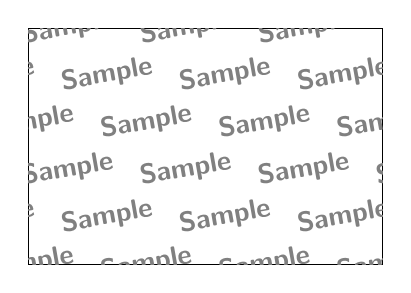
\begin{tikzpicture}
    \draw rectangle++(4.5,3);
    \clip rectangle++(4.5,3);
    \foreach\x in{0,1,2,3,4}{
      \foreach\y in{0,1,2,3,4,5,6}{
        \path(\x*1.5-\y*0.5,\y*0.6)node[rotate=10,text=gray]{\sffamily\bfseries\itshape Sample };
      }
    }
  \end{tikzpicture}
  %% 入れる画像：Ubuntu 24.04 にログインした直後のデスクトップ画面のスクリーンショット（上部バー、左側の Dock、アプリ一覧のボタンに番号を付ける）
  % eps 画像を貼る場合は includegraphics をお使いください。
  % 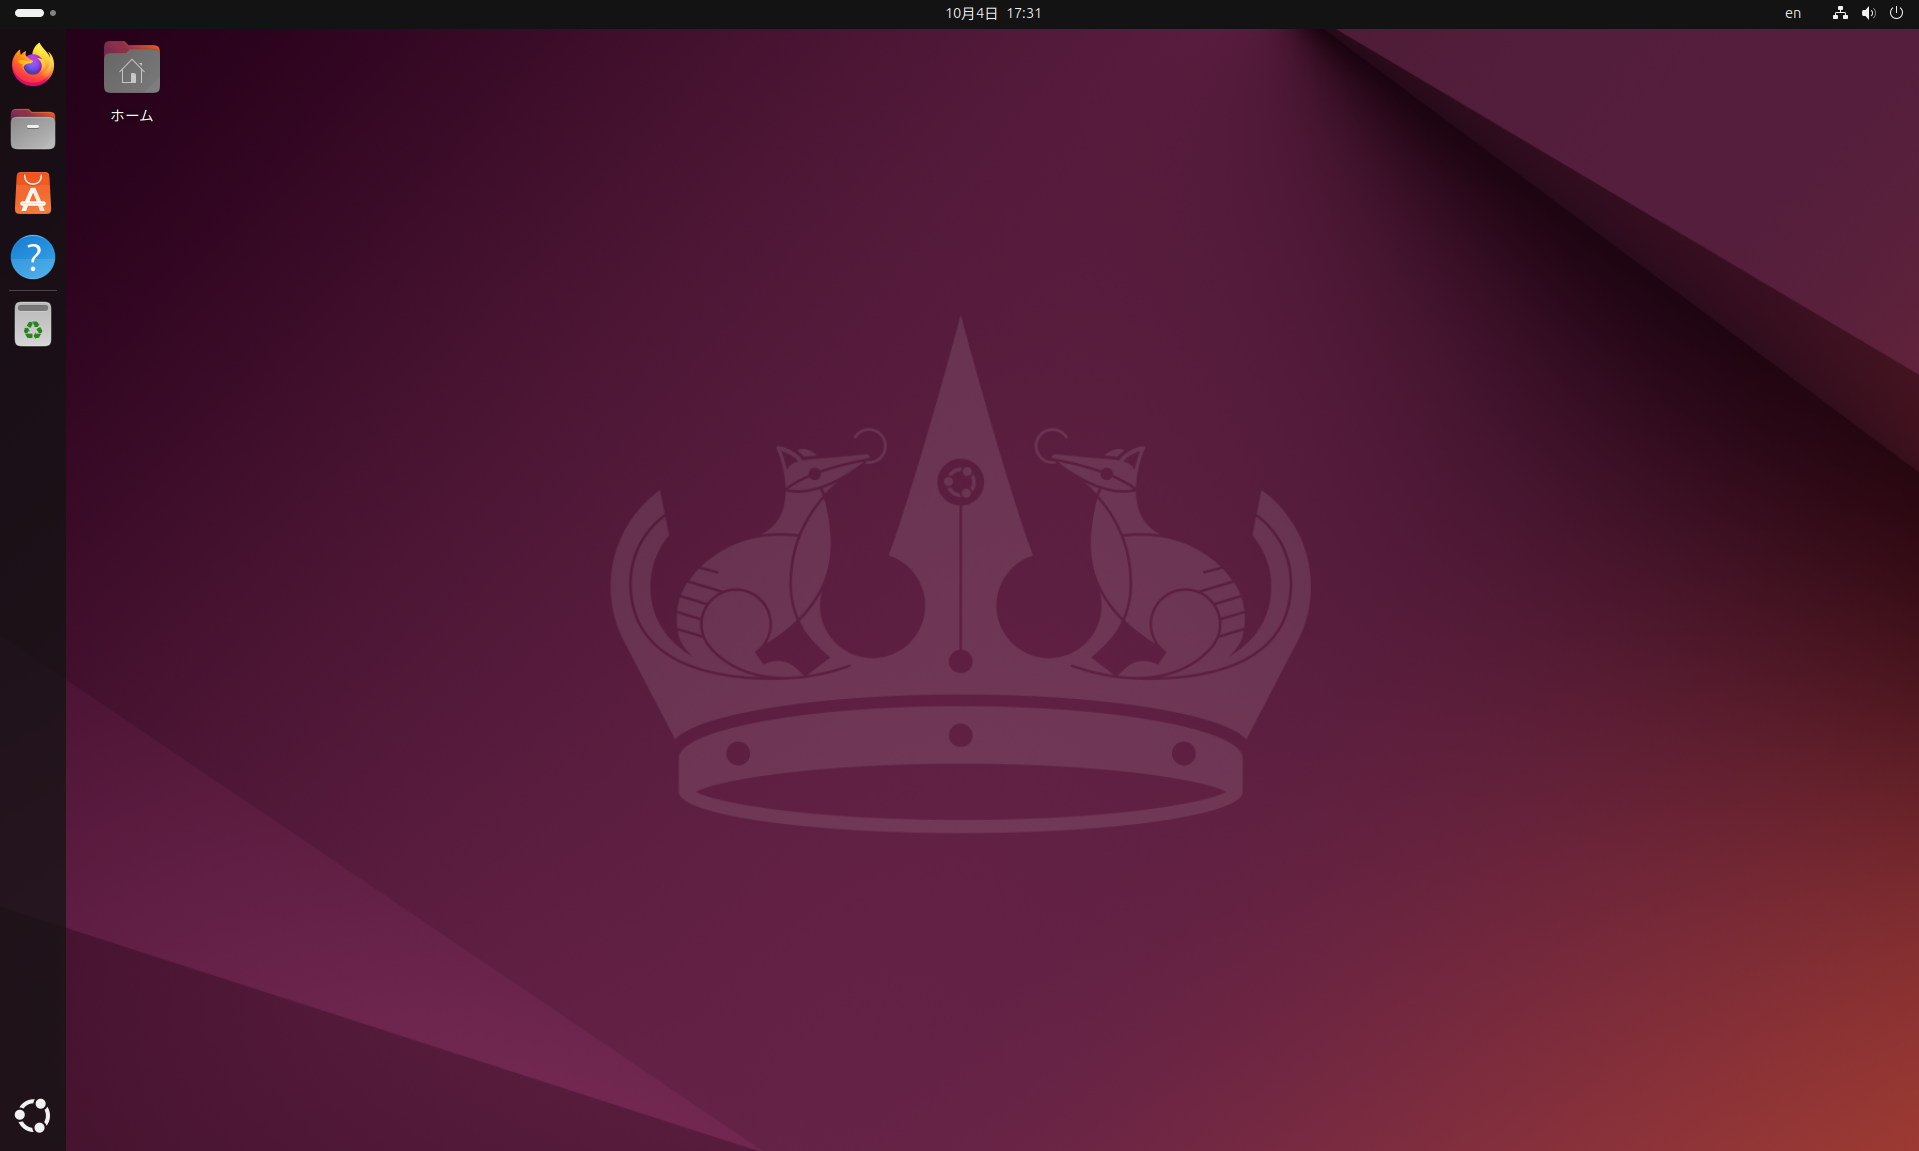
\includegraphics[width=0.8\linewidth]{what_is_linux/desktop.png}
  \caption{Ubuntu 24.04 のデスクトップ}
  \label{fig:linux-desktop}
\end{figure}

\subsection{画面の構成}

\begin{description}
  \item[上部バー]
    画面の上端にあるバーです。
    左端の「アクティビティ」を押すと、開いているウィンドウの一覧と検索画面が表示されます。
    中央には日付と時刻が、右端には、ネットワークや音量、電源などを操作するシステムメニューがあります。
  \item[Dock]
    画面の左端に並んでいるアイコンです。
    よく使うアプリケーションを起動したり、起動中のアプリケーションを切り替えたりできます。
    一番下のボタンを押すと、インストールされているすべてのアプリケーションの一覧が表示されます。
  \item[ワークスペース]
    仮想的な画面を複数用意して、作業ごとに使い分けるしくみです。
    たとえば、1 つ目のワークスペースでエディタとターミナルを、2 つ目のワークスペースでシミュレータを開く、といった使い方ができます。
\end{description}

\subsection{よく使うアプリケーション}

\begin{description}
  \item[ファイル] ファイルやディレクトリを GUI で操作するファイルマネージャです（\ref{sec:terminal-gui-cui}節）。
  \item[端末] コマンドを入力するためのターミナルです（\ref{chap:terminal_shell}章）。本書で最もよく使うアプリケーションです。
  \item[設定] ネットワーク（Wi-Fi）、ディスプレイ、キーボード、言語、ユーザなどの設定を行います。
  \item[App Center] アプリケーションを検索してインストールできます（\ref{chap:package}章）。
  \item[Firefox] Web ブラウザです。
\end{description}

\subsection{便利なショートカットキー}

キーボードの \key{Super} キーは、Windows のロゴが描かれたキーのことです。
次のショートカットキーを覚えておくと、マウスを使わずに素早く操作できます。

\begin{center}
  \begin{tabular}{ll}
    \toprule
    キー & 動作 \\
    \midrule
    \key{Super} & アクティビティ画面を開く（続けて文字を入力するとアプリを検索できる） \\
    \key{Ctrl}+\key{Alt}+\key{T} & ターミナルを開く \\
    \key{Alt}+\key{Tab} & ウィンドウを切り替える \\
    \key{Super}+\key{\(\leftarrow\)} / \key{\(\rightarrow\)} & ウィンドウを画面の左半分 / 右半分に配置する \\
    \key{Super}+\key{\(\uparrow\)} & ウィンドウを最大化する \\
    \key{Super}+\key{L} & 画面をロックする \\
    \key{Print} & スクリーンショットを撮る \\
    \bottomrule
  \end{tabular}
\end{center}

ターミナルとエディタを画面の左右に並べて作業することが多いので、\key{Super}+\key{\(\leftarrow\)} / \key{\(\rightarrow\)} は特に便利です。

\begin{point}[日本語の入力]
  日本語を選んでインストールした場合、日本語入力のソフトウェア（Mozc）も使えるようになっています。
  日本語入力と英字入力は、\key{半角/全角} キーで切り替えます。
  ターミナルでコマンドを入力するときは、英字入力になっているかを確かめましょう。
  全角の文字やスペースが混ざると、コマンドは正しく動きません（\ref{sec:terminal-command-structure}節）。
\end{point}

\section*{この章のまとめ}

\begin{itemize}
  \item Linux は、1991 年に Linus Torvalds が公開したカーネルに、GNU プロジェクトのソフトウェアなどを組み合わせた、UNIX の流れをくむ OS です。
  \item 「1 つのことをうまくやる小さなプログラムを組み合わせる」という UNIX 哲学は、Linux のコマンドや ROS 2 の設計にも通じています。
  \item Linux は OSS であり、ソースコードを読み、改良し、共有する自由があります。他人のコードを使うときはライセンスを確認します。
  \item Linux カーネルにさまざまなソフトウェアを組み合わせて配布しているものをディストリビューションといいます。本書では Ubuntu 24.04 LTS を使います。
  \item ROS 2 が Ubuntu を中心に開発されていること、さまざまなハードウェアで動くこと、リモートから操作しやすいことなどから、ロボット開発では Linux が広く使われています。
  \item Ubuntu の環境は、専用の PC にインストールするのがおすすめです。手軽に試すなら、仮想マシンや WSL2 も使えます。
  \item Ubuntu 24.04 のデスクトップ環境は GNOME です。\key{Super} キーでアプリを検索し、\key{Ctrl}+\key{Alt}+\key{T} でターミナルを開きます。
\end{itemize}

\chapter{Linux の仕組み}
\label{chap:linux_internals}

% この章で学ぶこと
\begin{goalbox}
  \begin{itemize}
    \item TODO
  \end{itemize}
\end{goalbox}

\section{カーネルとユーザ空間}

TODO

\section{ファイルシステムとディレクトリ構成}

TODO

\section{ユーザとグループ、root 権限}

TODO

\section{プロセスとは}

TODO

\section{デバイスファイルと「すべてはファイル」という考え方}

TODO

\section*{この章のまとめ}

TODO


\part{コマンドラインの基本}
\chapter{ターミナルとシェル}
\label{chap:terminal_shell}

% この章で学ぶこと
\begin{goalbox}
  \begin{itemize}
    \item GUI と CUI（CLI）の違いと、ロボット開発で CUI が使われる理由
    \item ターミナル・シェル・コマンドがそれぞれ何をしているのか
    \item プロンプトの読み方とコマンドの基本的な構造
    \item わからないコマンドの使い方を自分で調べる方法
    \item 入力を楽にするキー操作（Tab 補完、履歴検索など）
  \end{itemize}
\end{goalbox}

\section{GUI と CUI}
\label{sec:terminal-gui-cui}

\ref{chap:what_is_linux}章では、Ubuntu のデスクトップ環境をマウスで操作しました。
ウィンドウやアイコン、ボタンを見ながらマウスでクリックして操作する方式を \textbf{GUI}（Graphical User Interface）といいます。
Windows や macOS、スマートフォンの画面操作も GUI です。

これに対して、キーボードから文字で命令（\textbf{コマンド}）を入力し、結果も文字で受け取る方式を \textbf{CUI}（Character User Interface）といいます。
コマンドを入力して操作することから、\textbf{CLI}（Command Line Interface）とも呼ばれます。
本書では、以降は主に CLI と呼ぶことにします。

たとえば「ホームディレクトリにある \cmd{Documents} ディレクトリの中身を見る」という操作は、GUI と CLI で次のように違います。

\begin{itemize}
  \item GUI：ファイルマネージャを開き、「Documents」のアイコンをダブルクリックする
  \item CLI：ターミナルに \cmd{ls \textasciitilde/Documents} と入力して \key{Enter} を押す
\end{itemize}

\begin{terminal}[CLI でディレクトリの中身を見る]
$ ls ~/Documents
memo.txt  report.pdf
\end{terminal}

\begin{figure}[tb]
  \centering
  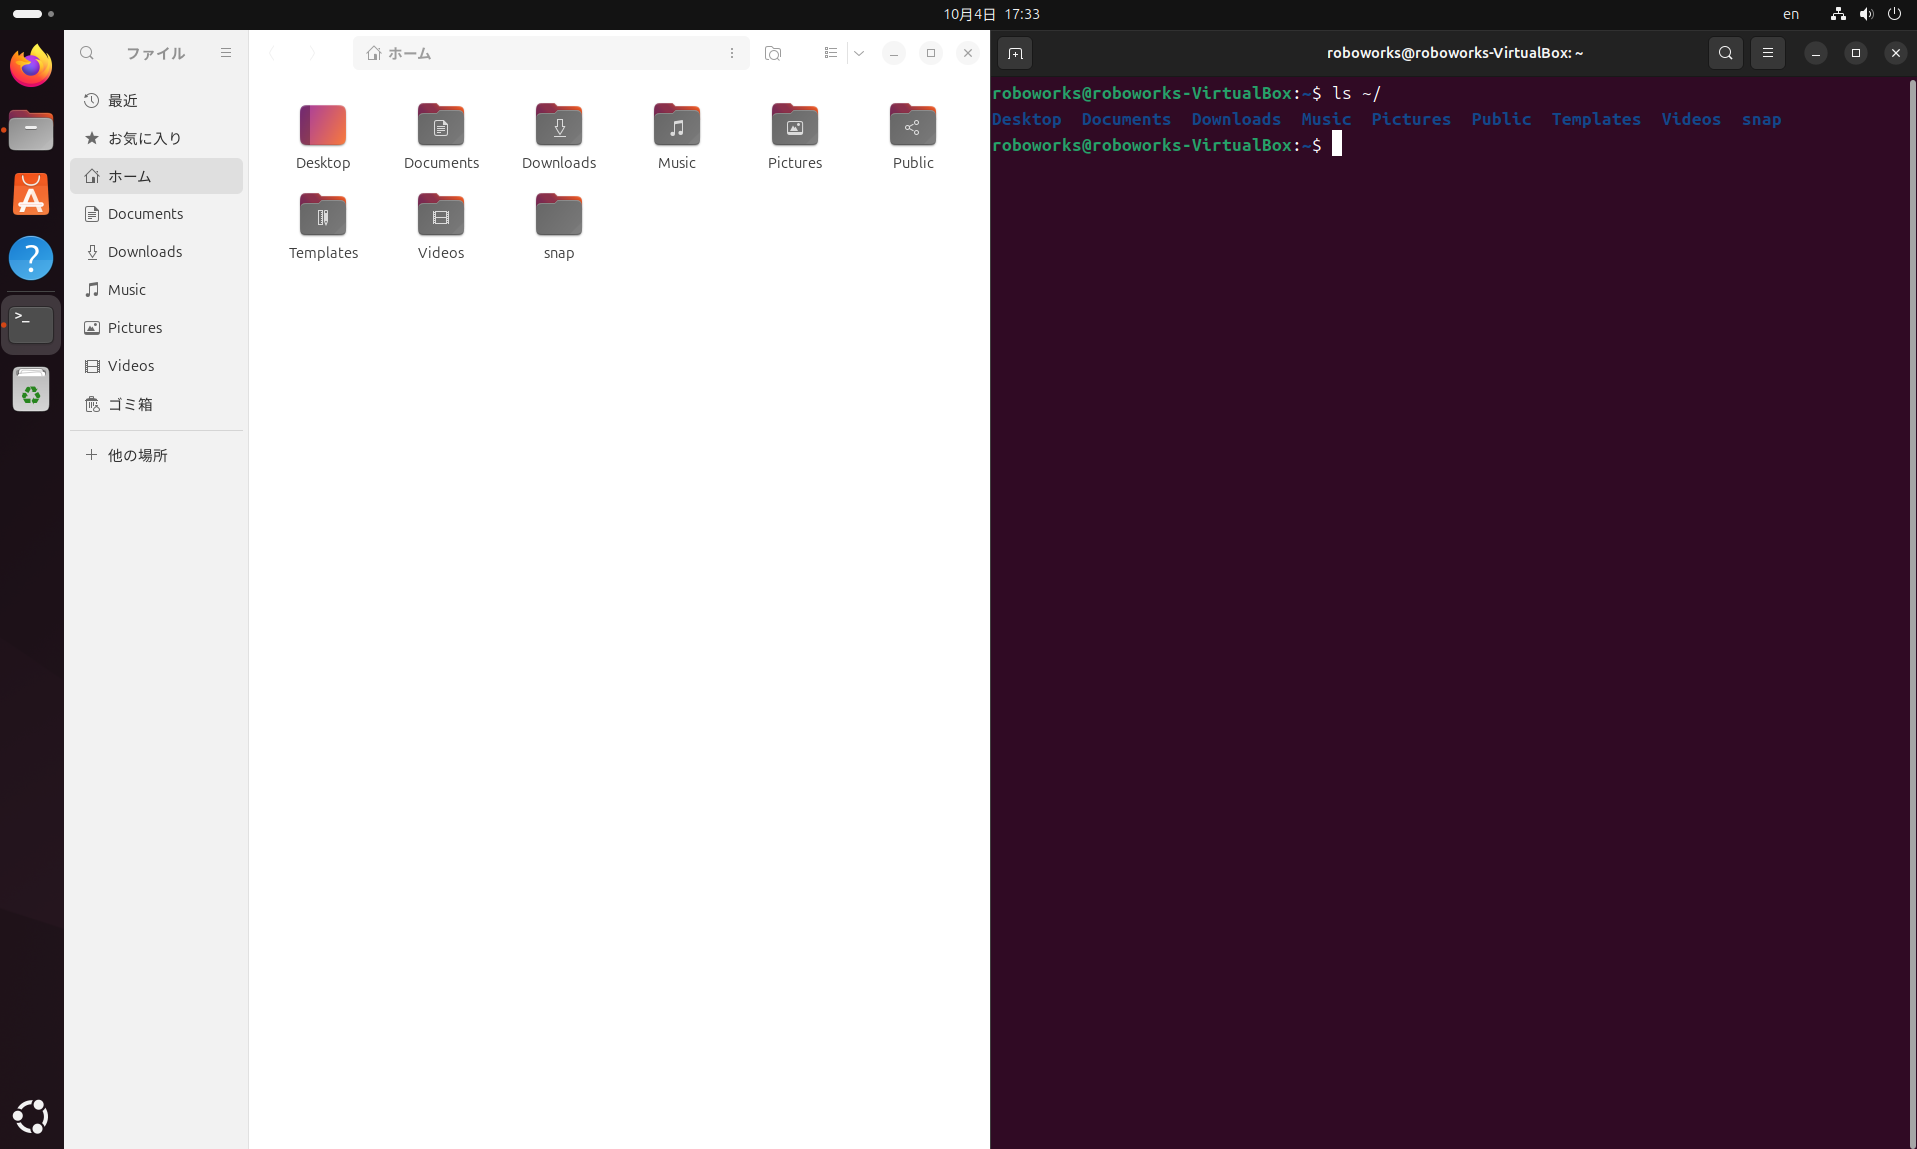
\includegraphics[width=0.9\linewidth]{terminal_shell/gui_vs_cli.png}
  \caption{同じディレクトリを GUI（左）と CLI（右）で表示した例}
  \label{fig:terminal-gui-cli}
\end{figure}

図\ref{fig:terminal-gui-cli}は、同じディレクトリをファイルマネージャとターミナルで表示したところです。
見た目はまったく違いますが、どちらも「ディレクトリの中身を一覧する」という同じ処理をコンピュータに頼んでいるだけです。
GUI のファイルマネージャも、裏側では CLI のコマンドと同じように OS の機能を呼び出しています。
つまり GUI と CLI は、同じコンピュータを操作するための 2 つの「窓口」だと考えることができます。

\subsection{CLI のよいところ}

初めて CLI を見ると、黒い画面に文字を打ち込む昔ながらの操作に見えるかもしれません。
それでもロボット開発の現場で CLI が使われ続けているのには、次のような理由があります。

\begin{description}
  \item[手順を正確に伝えられる]
    GUI の操作を人に伝えるには「右上のメニューから○○を選んで……」と言葉や画像で説明する必要があります。
    CLI なら、入力するコマンドをそのまま文字で渡せば、誰がやっても同じ結果になります。
    本書を含め、ROS の公式ドキュメントやインターネット上の情報の多くがコマンドで書かれているのはこのためです。
  \item[自動化できる]
    コマンドはファイルに書いておけば、まとめて何度でも実行できます（\ref{chap:shellscript}章で扱うシェルスクリプト）。
    毎回同じ手順を手で繰り返す必要がなくなり、操作ミスも減ります。
  \item[画面のないコンピュータを操作できる]
    ロボットに載っているコンピュータには、モニタがつながっていないことがよくあります。
    CLI なら、ネットワーク越しに別のコンピュータからログインして操作できます（\ref{chap:network}章で扱う SSH）。
  \item[軽くて速い]
    CLI は文字だけをやり取りするので、動作が軽く、性能の低いコンピュータや遅いネットワークでも快適に使えます。
    慣れてしまえば、マウスでメニューをたどるよりも速く操作できます。
  \item[ROS のツールの多くが CLI で提供されている]
    ROS 2 では、ノードの起動やトピックの確認などを \cmd{ros2} というコマンドで行います（\ref{chap:ros2_concepts}章）。
    ROS 2 を使うには、CLI に慣れておくことが欠かせません。
\end{description}

\subsection{GUI と CLI は使い分けるもの}

CLI が便利だからといって、GUI を使ってはいけないわけではありません。
画像や 3D モデルを見る、Web ページを閲覧する、ロボットのセンサデータを可視化する（\ref{chap:tf_viz}章で扱う RViz）といった作業は GUI のほうが向いています。

実際の開発では、「ファイルマネージャで画像を確認しながら、ターミナルでプログラムを実行する」というように、両方を行き来しながら作業します。
大切なのは、CLI を「怖いもの」「難しいもの」と思わずに、道具の 1 つとして選べるようになることです。

\begin{point}[GUI と CLI]
  \begin{itemize}
    \item GUI はマウスで画面を見ながら操作する方式、CLI はキーボードでコマンドを入力して操作する方式
    \item どちらも同じコンピュータを操作するための窓口で、できることの本質は変わらない
    \item ロボット開発では、手順の共有・自動化・リモート操作のしやすさから CLI がよく使われる
  \end{itemize}
\end{point}

\section{ターミナル・シェル・コマンドの関係}
\label{sec:terminal-relation}

それでは、実際に CLI を使ってみましょう。
Ubuntu では、\key{Ctrl}+\key{Alt}+\key{T} を押すと \textbf{ターミナル}が起動します。
アプリケーションの一覧から「端末」（英語表示では Terminal）を選んでも構いません。

\begin{terminal}[ターミナルを起動した直後の画面]
user@robot:~$
\end{terminal}

\begin{figure}[tb]
  \centering
  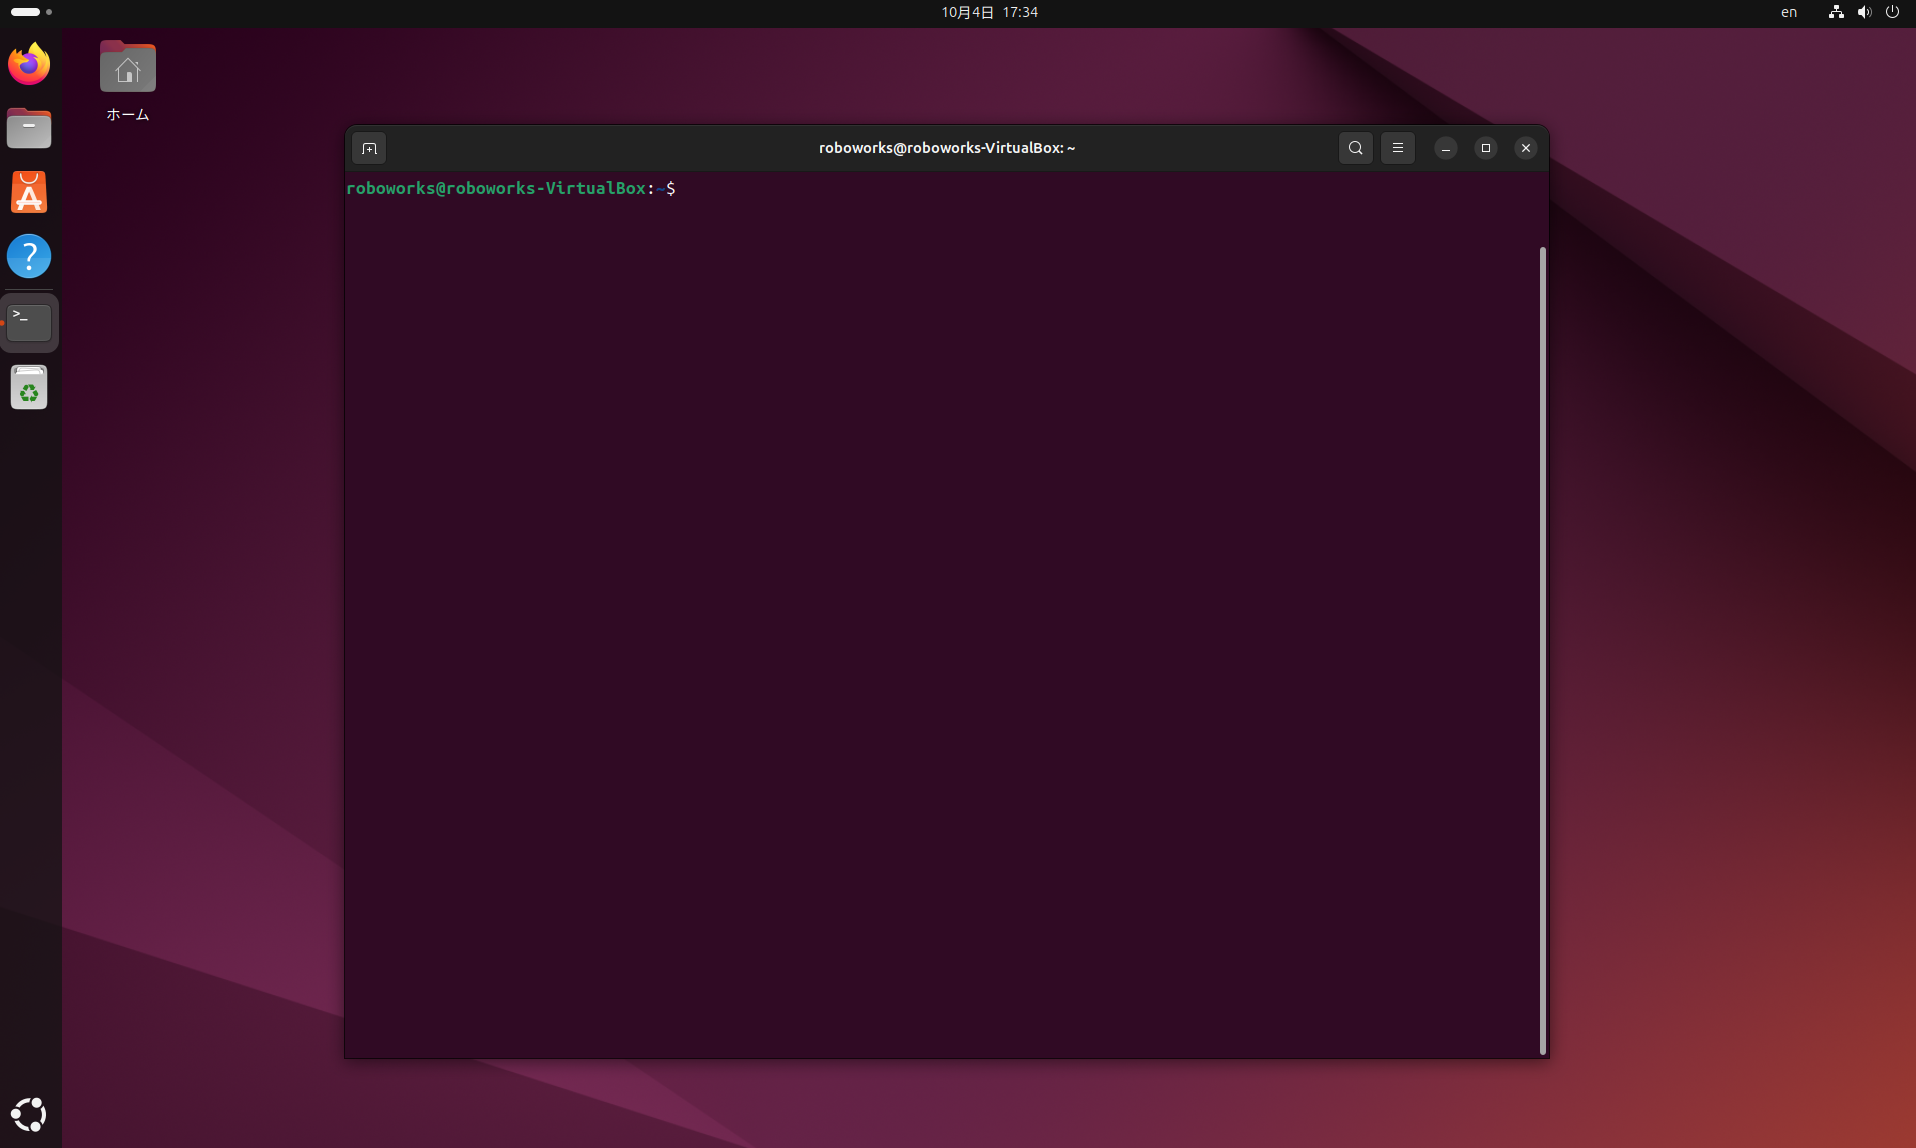
\includegraphics[width=0.9\linewidth]{terminal_shell/terminal_window.png}
  \caption{Ubuntu のターミナル}
  \label{fig:terminal-window}
\end{figure}

実際のターミナルは、図\ref{fig:terminal-window}のようなウィンドウです。
この画面に文字を入力して \key{Enter} を押すと、コンピュータが命令を実行して結果を表示してくれます。
試しに \cmd{date} と入力して \key{Enter} を押してみましょう。

\begin{terminal}[はじめてのコマンド]
$ date
Tue Sep 29 18:33:12 JST 2026
\end{terminal}

現在の日時が表示されれば成功です。
このとき裏側では、\textbf{ターミナル}・\textbf{シェル}・\textbf{コマンド}という 3 つのものが協力して動いています。

\begin{description}
  \item[ターミナル]
    キーボードからの入力を受け取り、文字を画面に表示するアプリケーションです。
    いわば文字の入出力を担当する「窓」で、ターミナル自身はコマンドの意味を理解していません。
    Ubuntu に標準で入っているのは GNOME Terminal ですが、ほかにも多くのターミナルアプリがあります。
  \item[シェル]
    ターミナルから受け取った文字列を解釈し、どのプログラムをどのように実行するかを決めるプログラムです。
    人間と OS（カーネル）の間に立つ「殻（shell）」なので、この名前がついています。
    Ubuntu で標準的に使われるシェルは \textbf{bash}（Bourne Again SHell）です。
  \item[コマンド]
    実際に仕事をするプログラムです。
    \cmd{date} は日時を表示するプログラム、\cmd{ls} はファイルの一覧を表示するプログラムです。
\end{description}

\cmd{date} と入力してから結果が表示されるまでの流れは、次のようになります。

\begin{enumerate}
  \item ターミナルが、キーボードから入力された \cmd{date} という文字列をシェルに渡す
  \item シェルが文字列を解釈し、\cmd{date} というプログラムを探して実行する
  \item \cmd{date} プログラムが現在の日時を調べて出力する
  \item ターミナルが、その出力を画面に表示する
\end{enumerate}

\begin{figure}[tb]
  \centering
  % 図：ターミナル・シェル・コマンドの関係（chapters/commandline/terminal_shell.tex）
\begin{tikzpicture}
  \node[font=\small, minimum height=14mm] (user) at (0,0) {利用者};
  \node[figpart, minimum width=19mm, minimum height=14mm] (term) at (2.4,0) {\textbf{ターミナル}\\{\footnotesize 入出力の窓}};
  \node[figpart, minimum width=19mm, minimum height=14mm] (shell) at (5.6,0) {\textbf{シェル}\\{\footnotesize bash}};
  \node[figpart, minimum width=19mm, minimum height=14mm, fill=orange!10] (cmd) at (8.8,0) {\textbf{コマンド}\\{\footnotesize date など}};
  % 行き
  \draw[figarrow] ([yshift=3mm]user.east) -- node[figlabel, above]{入力} ([yshift=3mm]term.west);
  \draw[figarrow] ([yshift=3mm]term.east) -- node[figlabel, above]{\tikz\node[fignum]{1}; 文字列} ([yshift=3mm]shell.west);
  \draw[figarrow] ([yshift=3mm]shell.east) -- node[figlabel, above]{\tikz\node[fignum]{2}; 実行} ([yshift=3mm]cmd.west);
  % 帰り
  \draw[figarrow] (cmd.south) -- ++(0,-0.6) -| node[figlabel, pos=0.25, below]{\tikz\node[fignum]{3}; 実行結果を出力} (term.south);
  \draw[figarrow] ([yshift=-3mm]term.west) -- node[figlabel, below]{\tikz\node[fignum]{4}; 表示} ([yshift=-3mm]user.east);
\end{tikzpicture}

  \caption{ターミナル・シェル・コマンドの関係}
  \label{fig:terminal-shell-command}
\end{figure}

この関係を図にすると、図\ref{fig:terminal-shell-command}のようになります。
レストランにたとえると、ターミナルは注文を聞いて料理を運ぶ「客席とテーブル」、シェルは注文を厨房に伝える「ホール係」、コマンドは実際に料理を作る「料理人」にあたります。

自分が使っているシェルは、次のコマンドで確認できます。
\cmd{\$SHELL} は、ログイン時に使うシェルを表す\textbf{環境変数}です（環境変数は\ref{chap:env}章で詳しく扱います）。

\begin{terminal}[使っているシェルを確認する]
$ echo $SHELL
/bin/bash
\end{terminal}

\cmd{echo} は、後ろに書いた文字列をそのまま表示するコマンドです。
シェルが \cmd{\$SHELL} を中身の \cmd{/bin/bash} に置き換えてから \cmd{echo} に渡すので、このような結果になります。

\subsection{コマンドの正体}

コマンドの多くは、ディレクトリに置かれたプログラムのファイルです。
\cmd{which} コマンドを使うと、コマンドのファイルがどこにあるかがわかります。

\begin{terminal}[コマンドのファイルの場所を調べる]
$ which date
/usr/bin/date
$ which ls
/usr/bin/ls
\end{terminal}

\cmd{date} の正体は \cmd{/usr/bin/date} というファイルだとわかりました。
ただし、\cmd{cd} のように、シェル自身に組み込まれているコマンド（\textbf{ビルトインコマンド}）もあります。
\cmd{type} コマンドを使うと、そのコマンドがどちらなのかを確認できます。

\begin{terminal}[コマンドの種類を調べる]
$ type date
date is /usr/bin/date
$ type cd
cd is a shell builtin
\end{terminal}

普段の操作で両者の違いを意識する必要はほとんどありませんが、後で説明するヘルプの調べ方が少し変わります。

\begin{column}{「端末」という言葉}
  ターミナル（terminal）は、もともとは大型のコンピュータにつながっていた、キーボードとディスプレイ（さらに昔はプリンタ）だけの「端末装置」を指す言葉でした。
  いまのターミナルアプリは、その端末装置をソフトウェアで再現したものなので、正確には\textbf{ターミナルエミュレータ}と呼ばれます。
  Ubuntu の日本語環境ではアプリ名が「端末」と表示されますが、本書では「ターミナル」と呼ぶことにします。
\end{column}

\section{プロンプトの読み方}
\label{sec:terminal-prompt}

ターミナルを起動すると、行の先頭に次のような文字列が表示されます。
これを\textbf{プロンプト}といい、「コマンドの入力を待っています」という合図です。

\begin{terminal}[プロンプト]
user@robot:~$
\end{terminal}

\begin{figure}[tb]
  \centering
  % 図：プロンプトの各部分の意味（chapters/commandline/terminal_shell.tex）
\begin{tikzpicture}[part/.style={font=\Large\ttfamily, text=white, inner sep=0pt, outer sep=0pt, anchor=base west}]
  \node[part] (u) at (0,0) {user};
  \node[part] (at) at (u.base east) {@};
  \node[part] (h) at (at.base east) {robot};
  \node[part] (c) at (h.base east) {:};
  \node[part] (d) at (c.base east) {\textasciitilde};
  \node[part] (p) at (d.base east) {\$};
  \begin{scope}[on background layer]
    \node[fill=black!85, rounded corners=2pt, inner xsep=3mm, inner ysep=2.5mm, fit=(u)(p)] (s) {};
  \end{scope}
  \draw[thick] (u.south |- s.south) -- ++(0,-0.6) node[below, figlabel]{ユーザ名};
  \draw[thick] (h.south |- s.south) -- ++(0,-1.5) node[below, figlabel]{ホスト名\\（コンピュータの名前）};
  \draw[thick] (d.south |- s.south) -- ++(0,-0.6) -- ++(0.9,0) node[right, figlabel, align=left]{カレントディレクトリ\\（\cmd{\textasciitilde} はホームディレクトリ）};
  \draw[thick] (p.north |- s.north) -- ++(0,0.5) -- ++(0.6,0) node[right, figlabel, align=left]{\cmd{\$}：一般ユーザ\\\cmd{\#}：root};
\end{tikzpicture}

  \caption{プロンプトの各部分の意味}
  \label{fig:terminal-prompt}
\end{figure}

Ubuntu の標準のプロンプトは、図\ref{fig:terminal-prompt}と次の表のような要素でできています。

\begin{tablebox}[プロンプトの各部分の意味][tab:terminal-prompt]
  \begin{tabular}{ll}
    \toprule
    部分 & 意味 \\
    \midrule
    \cmd{user} & ログインしているユーザ名 \\
    \cmd{@} & 区切り \\
    \cmd{robot} & コンピュータの名前（ホスト名） \\
    \cmd{:} & 区切り \\
    \cmd{\textasciitilde} & 今いるディレクトリ（\cmd{\textasciitilde} はホームディレクトリ） \\
    \cmd{\$} & 一般ユーザであることを表す記号 \\
    \bottomrule
  \end{tabular}
\end{tablebox}

ユーザ名とホスト名は、自分の環境に合わせて読み替えてください。
プロンプトに表示される情報は、次のコマンドでも確認できます。

\begin{terminal}[ユーザ名とホスト名を確認する]
$ whoami
user
$ hostname
robot
\end{terminal}

\subsection{今いるディレクトリ}

\cmd{:} と \cmd{\$} の間には、今いるディレクトリ（\textbf{カレントディレクトリ}）が表示されます。
\cmd{\textasciitilde} はホームディレクトリ（\cmd{/home/user}）を表す記号です。
別のディレクトリに移動すると、この部分が変わります。

\begin{terminal}[移動するとプロンプトが変わる]
user@robot:~$ cd /etc
user@robot:/etc$
\end{terminal}

ディレクトリの移動については、\ref{chap:files}章で詳しく説明します。
ネットワーク越しに複数のコンピュータを操作していると、今どのコンピュータのどのディレクトリで作業しているのかがわからなくなりがちです。
コマンドを入力する前にプロンプトを見る習慣をつけておくと、思わぬ事故を防げます。

\subsection{\$ と \#}

プロンプトの最後の記号は、一般ユーザなら \cmd{\$}、管理者（root）なら \cmd{\#} になります。
root はシステムのどんな設定でも変更できる特別なユーザです（\ref{chap:permission}章）。
プロンプトが \cmd{\#} になっているときは、操作を誤るとシステムを壊してしまう可能性があるので注意してください。

\begin{point}[本書でのコマンドの表記]
  本書のコマンド例では、プロンプトを省略して、一般ユーザで実行するコマンドの先頭に \cmd{\$}、root 権限で実行するコマンドの先頭に \cmd{\#} を付けています。
  \cmd{\$} や \cmd{\#} は入力せず、その後ろの部分だけを入力してください。
  \cmd{\$} や \cmd{\#} が付いていない行は、コマンドの実行結果です。
\end{point}

\begin{terminal}[本書の表記例]
$ echo Hello    # 「echo Hello」と入力する
Hello           # 実行結果（この行は入力しない）
\end{terminal}

\begin{caution}[表示される言語について]
  Ubuntu を日本語でインストールした場合、コマンドの実行結果やエラーメッセージが日本語で表示されることがあります。
  本書では英語の表示で掲載していますが、内容は同じです。
  なお、エラーメッセージをインターネットで検索するときは、英語のメッセージのほうが多くの情報が見つかります。
\end{caution}

\section{コマンドの構造}
\label{sec:terminal-command-structure}

コマンドは、基本的に次の形で入力します。
それぞれの間は半角スペースで区切ります。
\begin{terminal}[コマンドの基本形]
\begin{terminal}
$ コマンド名 オプション 引数
\end{terminal}

\begin{description}
  \item[コマンド名] 実行するプログラムの名前です（\cmd{ls}, \cmd{date} など）。
  \item[オプション] コマンドの動作を変える指定です。\cmd{-} や \cmd{--} で始まります。
  \item[引数] コマンドが処理する対象です。ファイル名やディレクトリ名などを指定します。
\end{description}

オプションや引数は、必要がなければ省略できます。
ファイルの一覧を表示する \cmd{ls} コマンドで試してみましょう。

\begin{terminal}[オプションと引数]
$ ls
Desktop  Documents  Downloads  Music  Pictures  Public  Templates  Videos
$ ls -l Documents
total 8
-rw-rw-r-- 1 user user   42 Sep 29 18:40 memo.txt
-rw-rw-r-- 1 user user 3120 Sep 29 18:41 report.pdf
\end{terminal}

1 つ目の \cmd{ls} は、オプションも引数もなしで実行しています。
この場合、カレントディレクトリの中身が表示されます。
2 つ目の \cmd{ls -l Documents} では、\cmd{-l}（詳しい情報を表示する）というオプションと、\cmd{Documents} という引数を指定しています。

\subsection{短いオプションと長いオプション}

オプションには、\cmd{-} とアルファベット 1 文字で書く\textbf{短いオプション}と、\cmd{--} と単語で書く\textbf{長いオプション}があります。
同じ意味のオプションに、両方の書き方が用意されていることもよくあります。

\begin{terminal}[同じ意味の短いオプションと長いオプション]
$ ls -a
$ ls --all
\end{terminal}

短いオプションは、まとめて書くこともできます。
次の 3 つは、どれも同じ意味です。

\begin{terminal}[短いオプションをまとめる]
$ ls -l -a
$ ls -la
$ ls -al
\end{terminal}

長いオプションは入力が長くなりますが、意味がわかりやすいので、スクリプトに書くときや人に説明するときに便利です。

\subsection{値をとるオプション}

オプションの中には、値を指定するものもあります。
たとえば、ファイルの先頭部分を表示する \cmd{head} コマンドでは、\cmd{-n} オプションで表示する行数を指定します。

\begin{terminal}[値をとるオプション]
$ head -n 3 /etc/os-release
PRETTY_NAME="Ubuntu 24.04.1 LTS"
NAME="Ubuntu"
VERSION_ID="24.04"
\end{terminal}

長いオプションで値を指定するときは、\cmd{--lines=3} のように \cmd{=} でつなぐのが一般的です。

\subsection{コマンド入力のルール}

コマンドを入力するときは、次の点に気をつけてください。

\begin{itemize}
  \item \textbf{大文字と小文字は区別されます。}\cmd{ls} と \cmd{LS} は別のものとして扱われます。
  \item \textbf{区切りは半角スペースです。}全角スペースを入れると、コマンドが正しく認識されません。
  \item \textbf{スペースを含む引数はクォートで囲みます。}\cmd{"my file.txt"} のようにダブルクォートで囲まないと、\cmd{my} と \cmd{file.txt} の 2 つの引数だと解釈されます。
\end{itemize}

存在しないコマンドを入力すると、次のようなメッセージが表示されます。

\begin{terminal}[コマンドが見つからない]
$ LS
LS: command not found
\end{terminal}

\cmd{command not found} と表示されたら、まずはスペルミスや大文字・小文字の間違いがないかを確認しましょう。
Ubuntu では、打ち間違えたコマンドの候補や、インストールすれば使えるパッケージを教えてくれることもあります。

\begin{point}[便りがないのはよい便り]
  CLI のコマンドの多くは、成功したときには何も表示しません。
  たとえば、ディレクトリを作る \cmd{mkdir} コマンドは、成功すると何も言わずに次のプロンプトを表示します。
  何も表示されなかったら「失敗した」のではなく、「うまくいった」と考えてください。
  失敗したときには、必ずエラーメッセージが表示されます。
\end{point}

\section{ヘルプの調べ方}
\label{sec:terminal-help}

Linux には非常にたくさんのコマンドがあり、それぞれに多くのオプションがあります。
それらをすべて覚える必要はありません。
大切なのは、\textbf{わからないときに自分で調べる方法}を知っておくことです。

\subsection{\cmd{-{}-help} オプション}

多くのコマンドは、\cmd{--help} オプションを付けて実行すると、使い方の要約を表示します。

\begin{terminal}[--help で使い方を表示する]
$ ls --help
Usage: ls [OPTION]... [FILE]...
List information about the FILEs (the current directory by default).
Sort entries alphabetically if none of -cftuvSUX nor --sort is specified.

Mandatory arguments to long options are mandatory for short options too.
  -a, --all                  do not ignore entries starting with .
  -A, --almost-all           do not list implied . and ..
...
\end{terminal}

1 行目の \cmd{Usage} は、コマンドの書き方を表しています。
\cmd{[ ]} で囲まれた部分は省略できること、\cmd{...} は複数指定できることを意味します。
つまり \cmd{ls [OPTION]... [FILE]...} は、「\cmd{ls} の後ろに、オプションとファイルをそれぞれ 0 個以上書ける」という意味です。

表示が長くて画面からあふれてしまうときは、\cmd{ls --help | less} のように入力すると、1 画面ずつ読めます（\cmd{|} については\ref{chap:text_pipe}章で説明します）。

\subsection{\cmd{man} コマンド}

より詳しい説明が必要なときは、\cmd{man} コマンドでマニュアル（\textbf{man ページ}）を読みます。

\begin{terminal}[ls のマニュアルを表示する]
$ man ls
\end{terminal}

\begin{figure}[tb]
  \centering
  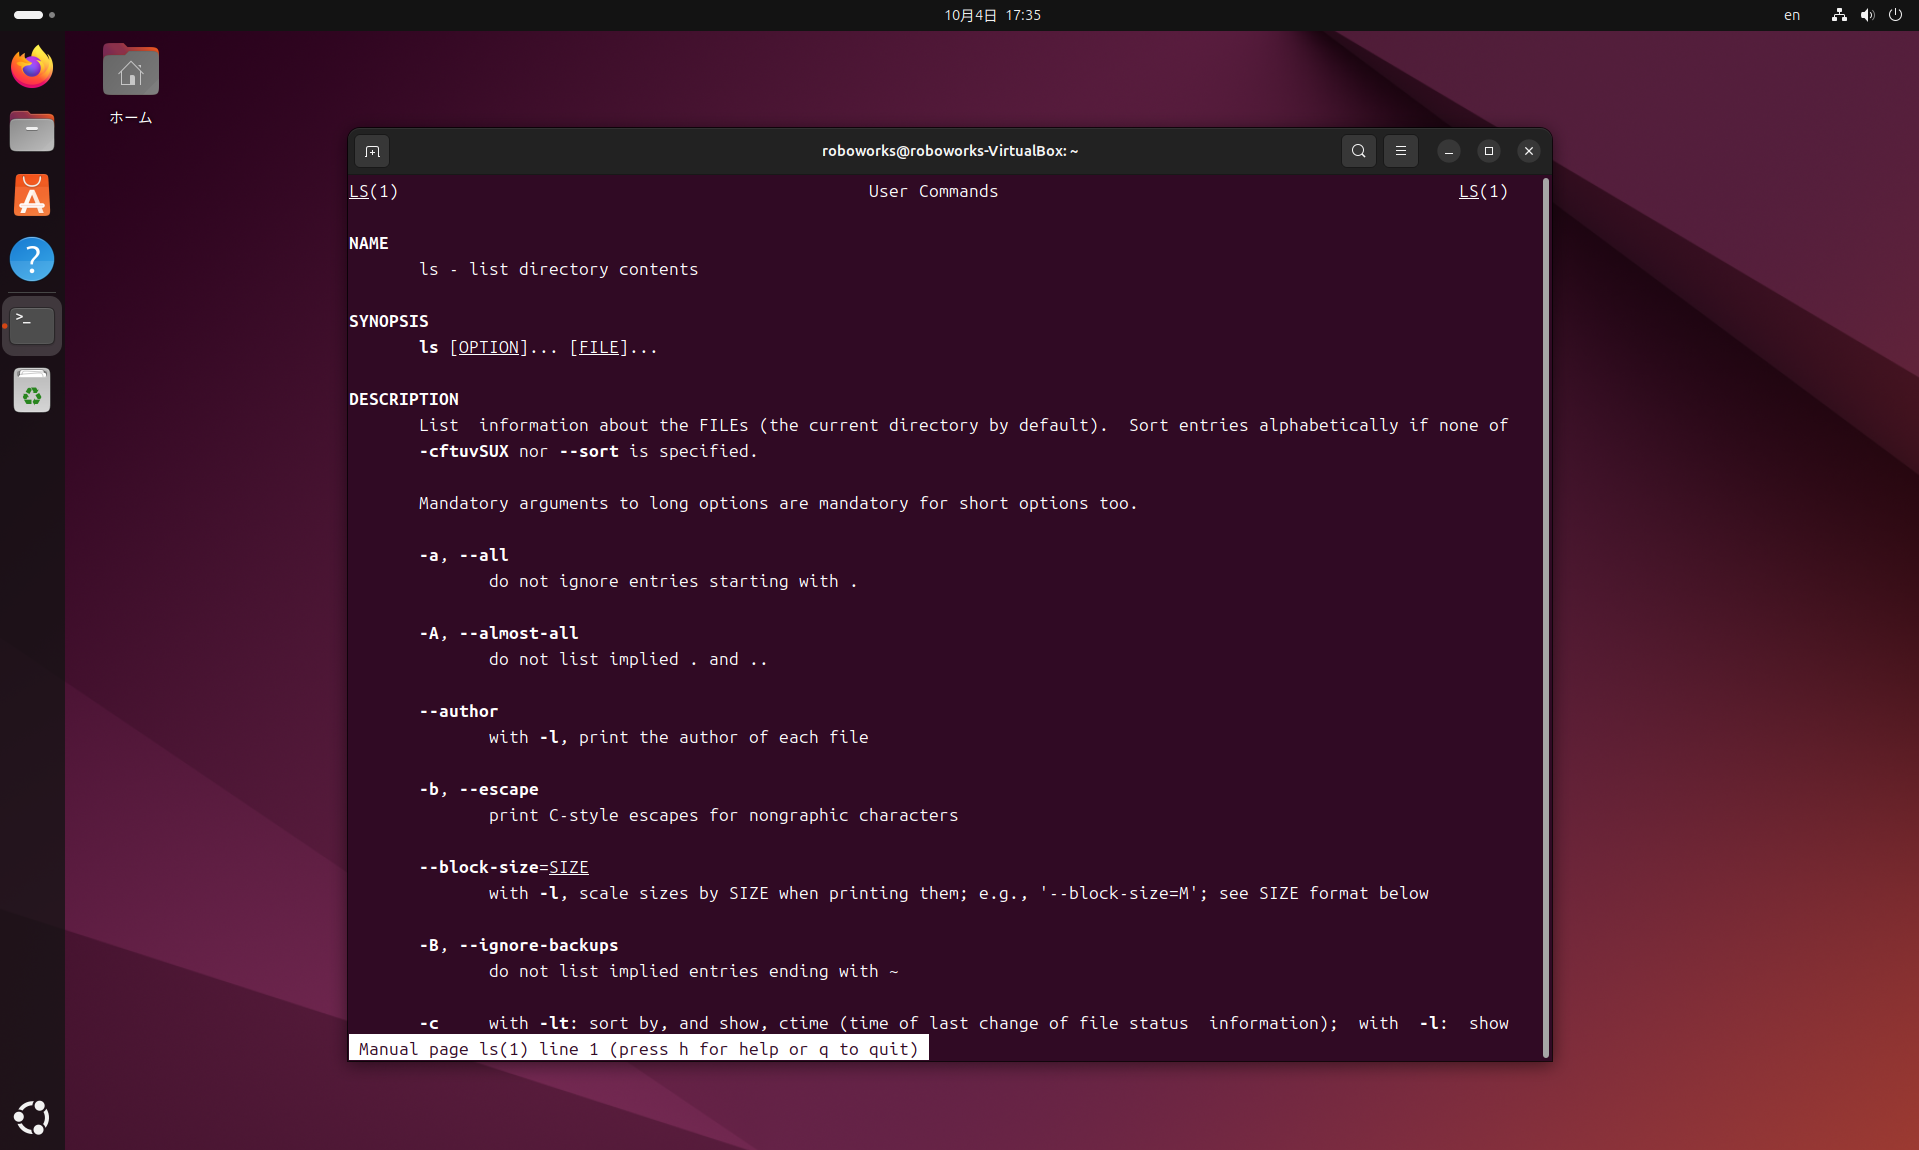
\includegraphics[width=0.9\linewidth]{terminal_shell/man_ls.png}
  \caption{\cmd{man ls} の表示画面}
  \label{fig:terminal-man}
\end{figure}

\cmd{man ls} を実行すると、図\ref{fig:terminal-man}のような画面が表示されます。
man ページは、次のキーで操作します。
特に、\textbf{終了するときは \key{q}} は必ず覚えておきましょう。

\begin{tablebox}[man ページの操作][tab:terminal-man-keys]
  \begin{tabular}{ll}
    \toprule
    キー & 動作 \\
    \midrule
    \key{Space} / \key{b} & 1 画面進む / 1 画面戻る \\
    \key{\(\downarrow\)} / \key{\(\uparrow\)} & 1 行進む / 1 行戻る \\
    \key{/} 文字列 & 文字列を検索する \\
    \key{n} / \key{N} & 次の検索結果 / 前の検索結果 \\
    \key{q} & 終了する \\
    \bottomrule
  \end{tabular}
\end{tablebox}

man ページは、おおむね次のような見出しで構成されています。

\begin{description}
  \item[NAME] コマンドの名前と一行説明
  \item[SYNOPSIS] コマンドの書き方（\cmd{--help} の \cmd{Usage} と同じ）
  \item[DESCRIPTION] 詳しい説明と、オプションの一覧
  \item[EXAMPLES] 使用例（ないコマンドもあります）
  \item[SEE ALSO] 関連するコマンド
\end{description}

最初から全部を読む必要はありません。
\key{/} で知りたいオプションを検索して、その部分だけを読むのが効率的です。

\begin{tips}{man ページが英語で読みにくいとき}
  man ページの多くは英語で書かれています。
  最初は読みにくいかもしれませんが、使われる単語はある程度決まっているので、読んでいるうちに慣れてきます。
  どうしても読みにくいときは、次に紹介する \cmd{tldr} を使ったり、Web ブラウザで「コマンド名 使い方」と検索したりするとよいでしょう。
\end{tips}

\subsection{\cmd{tldr} コマンド}

\cmd{tldr}（Too Long; Didn't Read の略）は、よく使う使用例だけを簡潔にまとめて表示してくれるコマンドです。
標準ではインストールされていないので、次のようにインストールします（\cmd{apt} については\ref{chap:package}章で説明します）。

\begin{terminal}[tldr をインストールする]
$ sudo apt install tldr
$ tldr --update
\end{terminal}

\cmd{tldr} の後ろにコマンド名を書くと、使用例が表示されます。

\begin{terminal}[tar コマンドの使用例を表示する]
$ tldr tar
tar
Archiving utility.

 - Create an archive and write it to a file:
   tar cf path/to/target.tar path/to/file1 path/to/file2 ...

 - Extract a (compressed) archive file into the current directory verbosely:
   tar xvf path/to/source.tar[.gz|.bz2|.xz]
...
\end{terminal}

「細かい説明はいいから、とりあえずよくある使い方を知りたい」というときに便利です。

\subsection{ビルトインコマンドのヘルプ}

\cmd{cd} のようなビルトインコマンドには、\cmd{man} ページがないことがあります。
その場合は、bash の \cmd{help} コマンドを使います。

\begin{terminal}[ビルトインコマンドのヘルプを表示する]
$ help cd
cd: cd [-L|[-P [-e]] [-@]] [dir]
    Change the shell working directory.
...
\end{terminal}

\begin{point}[ヘルプの調べ方のまとめ]
  \begin{itemize}
    \item まずは \cmd{コマンド名 --help} で使い方の要約を見る
    \item 詳しく知りたいときは \cmd{man コマンド名} でマニュアルを読む（終了は \key{q}）
    \item 使用例を知りたいときは \cmd{tldr コマンド名}
    \item ビルトインコマンドは \cmd{help コマンド名}
  \end{itemize}
\end{point}

\section{便利なキー操作}
\label{sec:terminal-keys}

CLI では、すべてをキーボードで入力する必要があります。
長いコマンドやファイル名を毎回すべて入力するのは大変ですが、シェルには入力を楽にするしくみがたくさん用意されています。
ここで紹介する操作を覚えるだけで、CLI の使い心地は大きく変わります。

\subsection{Tab 補完}

コマンド名やファイル名を途中まで入力して \key{Tab} を押すと、残りをシェルが自動的に入力してくれます。
これを \textbf{Tab 補完}といいます。

\begin{terminal}[Tab 補完]
$ cd Doc          # ここで Tab キーを押すと
$ cd Documents/   # 残りが自動で入力される
\end{terminal}

候補が複数あって 1 つに決まらないときは、何も起きません。
そのままもう一度 \key{Tab} を押すと、候補の一覧が表示されます。

\begin{terminal}[候補が複数あるとき（Tab を 2 回押す）]
$ cd D
Desktop/   Documents/ Downloads/
\end{terminal}

候補を絞り込めるところまで文字を追加して、もう一度 \key{Tab} を押しましょう。

Tab 補完を使うと入力が速くなるだけでなく、\textbf{打ち間違いを防げる}という大きな利点があります。
補完されないということは、そのファイルやディレクトリが存在しないか、途中までの入力が間違っているということです。
ファイル名を入力するときは、常に Tab 補完を使う習慣をつけましょう。

\subsection{コマンド履歴}

シェルは、過去に入力したコマンドを\textbf{履歴}として記録しています。
\key{\(\uparrow\)} を押すと 1 つ前のコマンドが、さらに押すとその前のコマンドが呼び出されます。
\key{\(\downarrow\)} で新しい方向に戻ります。
呼び出したコマンドは、\key{\(\leftarrow\)} \key{\(\rightarrow\)} でカーソルを動かして編集してから実行することもできます。

履歴の一覧は \cmd{history} コマンドで表示できます。

\begin{terminal}[コマンド履歴を表示する]
$ history
    1  date
    2  echo $SHELL
    3  which date
    4  ls -l Documents
    5  history
\end{terminal}

\subsection{履歴の検索}

ずっと前に入力したコマンドを \key{\(\uparrow\)} でたどるのは大変です。
そんなときは \key{Ctrl}+\key{R} を押して、コマンドの一部を入力します。
入力した文字列を含むコマンドが、新しいものから順に検索されます。

\begin{terminal}[Ctrl+R で履歴を検索する]
(reverse-i-search)`ls': ls -l Documents
\end{terminal}

\key{Ctrl}+\key{R} を続けて押すと、さらに古い候補に移ります。
見つかったら \key{Enter} でそのまま実行し、編集したいときは \key{\(\leftarrow\)} や \key{\(\rightarrow\)} を押してから編集します。
検索をやめるときは \key{Ctrl}+\key{G} を押します。

ROS 2 では長いコマンドを何度も入力することが多いので、\key{Ctrl}+\key{R} は特に役立ちます。

\subsection{実行中のコマンドを止める}

コマンドの中には、止めるまで動き続けるものがあります。
ROS 2 のノードも、基本的には止めるまで動き続けます。
実行中のコマンドを止めるには、\key{Ctrl}+\key{C} を押します。

\begin{terminal}[Ctrl+C でコマンドを止める]
$ ping localhost
PING localhost (127.0.0.1) 56(84) bytes of data.
64 bytes from localhost (127.0.0.1): icmp_seq=1 ttl=64 time=0.030 ms
64 bytes from localhost (127.0.0.1): icmp_seq=2 ttl=64 time=0.045 ms
^C
--- localhost ping statistics ---
2 packets transmitted, 2 received, 0% packet loss, time 1001ms
\end{terminal}

\cmd{\textasciicircum C} は、\key{Ctrl}+\key{C} を押したことを表しています。

\begin{caution}[コピーは Ctrl+C ではない]
  ターミナルでは \key{Ctrl}+\key{C} が「コマンドを止める」操作に割り当てられているため、コピーには使えません。
  ターミナルで文字をコピー・貼り付けするときは、\key{Ctrl}+\key{Shift}+\key{C} と \key{Ctrl}+\key{Shift}+\key{V} を使います。
  Web ページなどからコマンドを貼り付けるときは、意図しないコマンドが含まれていないかを確認してから \key{Enter} を押しましょう。
\end{caution}

\subsection{その他の便利なキー操作}

ほかにも、次のようなキー操作がよく使われます。
最初からすべてを覚える必要はないので、必要になったときにこの表を見返してください。

\begin{tablebox}[ターミナルで便利なキー操作][tab:terminal-keys]
  \begin{tabular}{lp{0.45\linewidth}}
    \toprule
    キー & 動作 \\
    \midrule
    \key{Tab} & コマンド名・ファイル名を補完する \\
    \key{\(\uparrow\)} / \key{\(\downarrow\)} & 履歴をたどる \\
    \key{Ctrl}+\key{R} & 履歴を検索する \\
    \key{Ctrl}+\key{C} & 実行中のコマンドを止める \\
    \key{Ctrl}+\key{D} & シェルを終了する（入力の終わりを伝える） \\
    \key{Ctrl}+\key{L} & 画面をきれいにする（\cmd{clear} と同じ） \\
    \key{Ctrl}+\key{A} / \key{Ctrl}+\key{E} & カーソルを行頭 / 行末に移動する \\
    \key{Ctrl}+\key{U} & カーソルより前をすべて消す \\
    \key{Ctrl}+\key{K} & カーソルより後ろをすべて消す \\
    \key{Ctrl}+\key{Shift}+\key{C} / \key{V} & コピー / 貼り付け \\
    \bottomrule
  \end{tabular}
\end{tablebox}

ターミナルを閉じるときは、ウィンドウの閉じるボタンを押すか、\cmd{exit} と入力します。

\section*{この章のまとめ}

\begin{itemize}
  \item GUI はマウスで、CLI はキーボードからコマンドを入力してコンピュータを操作する方式です。ロボット開発では、手順の共有・自動化・リモート操作のしやすさから CLI がよく使われます。
  \item ターミナルは文字の入出力を担当するアプリ、シェルは入力を解釈してコマンドを実行するプログラム、コマンドは実際に仕事をするプログラムです。
  \item プロンプト \cmd{user@robot:\textasciitilde\$} には、ユーザ名・ホスト名・カレントディレクトリが表示されます。
  \item コマンドは「コマンド名 オプション 引数」の形で入力します。
  \item 使い方がわからないときは \cmd{--help}、\cmd{man}、\cmd{tldr} で調べます。
  \item Tab 補完、\key{\(\uparrow\)}、\key{Ctrl}+\key{R}、\key{Ctrl}+\key{C} を使いこなすと、CLI の操作がぐっと楽になります。
\end{itemize}

\chapter{ファイルとディレクトリの操作}
\label{chap:files}

% この章で学ぶこと
\begin{goalbox}
  \begin{itemize}
    \item カレントディレクトリの確認と移動（\cmd{pwd}, \cmd{cd}, \cmd{ls}）
    \item 絶対パスと相対パスの考え方
    \item ファイルやディレクトリの作成・コピー・移動・削除
    \item ファイルの中身の確認と、テキストエディターによる編集、ファイルの探し方
    \item ワイルドカードとブレース展開を使った効率的な指定方法
  \end{itemize}
\end{goalbox}

ふだん GUI のファイルマネージャで行っている「フォルダを開く」「ファイルをコピーする」「ゴミ箱に捨てる」といった操作は、すべて CLI でも行えます。
この章では、ファイルとディレクトリを操作する基本的なコマンドを学びます。
ここで学ぶコマンドは、ROS 2 のワークスペースを作ったりプログラムを編集したりするときに毎日のように使うものばかりです。

\section{現在地の確認と移動}
\label{sec:files-navigation}

\begin{figure}[tb]
  \centering
  % 図：Linux のディレクトリ構成（一部）（chapters/commandline/files.tex）
% このファイルは手で編集して構いません（行を増やすときは y 座標と縦線に注意）
\begin{tikzpicture}[every node/.style={inner sep=1.5pt}]
  \node[anchor=west, font=\small\ttfamily] (n0) at (0.00,0.00) {/};
  \node[anchor=west, font=\footnotesize, text=black!60] at (4.2,0.00) {ルートディレクトリ};
  \draw[black!25, dotted] (n0.east) -- (4.15,0.00);
  \node[anchor=west, font=\small\ttfamily] (n1) at (0.70,-0.48) {bin/};
  \draw[black!50] (0.15,-0.20) |- (n1.west);
  \node[anchor=west, font=\small\ttfamily] (n2) at (0.70,-0.96) {etc/};
  \draw[black!50] (0.15,-0.20) |- (n2.west);
  \node[anchor=west, font=\footnotesize, text=black!60] at (4.2,-0.96) {設定ファイル};
  \draw[black!25, dotted] (n2.east) -- (4.15,-0.96);
  \node[anchor=west, font=\small\ttfamily] (n3) at (0.70,-1.44) {home/};
  \draw[black!50] (0.15,-0.20) |- (n3.west);
  \node[anchor=west, font=\small\ttfamily, fill=blue!10] (n4) at (1.40,-1.92) {user/};
  \draw[black!50] (0.85,-1.64) |- (n4.west);
  \node[anchor=west, font=\footnotesize, text=black!60] at (4.2,-1.92) {ホームディレクトリ（\cmd{\textasciitilde}）};
  \draw[black!25, dotted] (n4.east) -- (4.15,-1.92);
  \node[anchor=west, font=\small\ttfamily] (n5) at (2.10,-2.40) {Desktop/};
  \draw[black!50] (1.55,-2.12) |- (n5.west);
  \node[anchor=west, font=\small\ttfamily] (n6) at (2.10,-2.88) {Documents/};
  \draw[black!50] (1.55,-2.12) |- (n6.west);
  \node[anchor=west, font=\small\ttfamily] (n7) at (2.80,-3.36) {memo.txt};
  \draw[black!50] (2.25,-3.08) |- (n7.west);
  \node[anchor=west, font=\small\ttfamily] (n8) at (2.10,-3.84) {Downloads/};
  \draw[black!50] (1.55,-2.12) |- (n8.west);
  \node[anchor=west, font=\small\ttfamily] (n9) at (0.70,-4.32) {opt/};
  \draw[black!50] (0.15,-0.20) |- (n9.west);
  \node[anchor=west, font=\small\ttfamily] (n10) at (1.40,-4.80) {ros/};
  \draw[black!50] (0.85,-4.52) |- (n10.west);
  \node[anchor=west, font=\small\ttfamily] (n11) at (2.10,-5.28) {jazzy/};
  \draw[black!50] (1.55,-5.00) |- (n11.west);
  \node[anchor=west, font=\footnotesize, text=black!60] at (4.2,-5.28) {ROS 2 Jazzy};
  \draw[black!25, dotted] (n11.east) -- (4.15,-5.28);
  \node[anchor=west, font=\small\ttfamily] (n12) at (0.70,-5.76) {usr/};
  \draw[black!50] (0.15,-0.20) |- (n12.west);
  \node[anchor=west, font=\small\ttfamily] (n13) at (1.40,-6.24) {bin/};
  \draw[black!50] (0.85,-5.96) |- (n13.west);
  \node[anchor=west, font=\footnotesize, text=black!60] at (4.2,-6.24) {コマンド};
  \draw[black!25, dotted] (n13.east) -- (4.15,-6.24);
  \node[anchor=west, font=\small\ttfamily] (n14) at (1.40,-6.72) {share/};
  \draw[black!50] (0.85,-5.96) |- (n14.west);
  \node[anchor=west, font=\small\ttfamily] (n15) at (0.70,-7.20) {tmp/};
  \draw[black!50] (0.15,-0.20) |- (n15.west);
  \node[anchor=west, font=\footnotesize, text=black!60] at (4.2,-7.20) {一時ファイル};
  \draw[black!25, dotted] (n15.east) -- (4.15,-7.20);
\end{tikzpicture}

  \caption{Linux のディレクトリ構成（一部）}
  \label{fig:files-tree}
\end{figure}

\ref{chap:linux_internals}章で説明したように、Linux のファイルは \cmd{/}（ルートディレクトリ）を頂点とする木構造で管理されています。
CLI で作業するときは、常にこの木構造のどこかのディレクトリに「いる」状態になります。
このディレクトリを\textbf{カレントディレクトリ}（作業ディレクトリ）といいます。
図\ref{fig:files-tree}に、Linux のディレクトリ構成の一部を示します。

\subsection{\cmd{pwd}：今いる場所を表示する}

\cmd{pwd}（print working directory）は、カレントディレクトリを表示するコマンドです。

\begin{terminal}[カレントディレクトリを表示する]
$ pwd
/home/user
\end{terminal}

ターミナルを起動した直後は、自分の\textbf{ホームディレクトリ}（\cmd{/home/ユーザ名}）にいます。
ホームディレクトリは、そのユーザが自由にファイルを置ける専用のディレクトリです。

本書では、ユーザ名を \cmd{user} として表示しています。
\cmd{user} の部分は、Ubuntu をインストールしたときに自分で決めたユーザ名になります（\ref{sec:linux-setup}節）。
たとえば、ユーザ名を \cmd{taro} にした場合は、\cmd{/home/taro} と表示されます。
以降の実行結果でも、\cmd{user} は自分のユーザ名に読み替えてください。

\subsection{\cmd{ls}：ディレクトリの中身を表示する}

\cmd{ls}（list）は、ディレクトリの中にあるファイルやディレクトリの一覧を表示します。
引数を省略するとカレントディレクトリの中身を、引数にディレクトリを指定するとそのディレクトリの中身を表示します。

\begin{terminal}[ディレクトリの中身を表示する]
$ ls
Desktop  Documents  Downloads  Music  Pictures  Public  snap  Templates  Videos
$ ls /
bin   dev  home  lib64  mnt  proc  run   snap  sys  usr
boot  etc  lib   media  opt  root  sbin  srv   tmp  var
\end{terminal}

\cmd{ls} には多くのオプションがありますが、まずは次の 3 つを覚えておきましょう。

\begin{tablebox}[\cmd{ls} のよく使うオプション][tab:files-ls-options]
  \begin{tabular}{lp{0.75\linewidth}}
    \toprule
    オプション & 意味 \\
    \midrule
    \cmd{-l} & 権限・サイズ・更新日時などの詳しい情報を表示する \\
    \cmd{-a} & \cmd{.} で始まる隠しファイルも表示する \\
    \cmd{-h} & \cmd{-l} と組み合わせ、サイズを K, M などの単位で表示する \\
    \bottomrule
  \end{tabular}
\end{tablebox}

\begin{terminal}[詳しい情報を表示する]
$ ls -lh
total 32K
drwxr-xr-x 2 user user 4.0K Sep 29 18:33 Desktop
drwxr-xr-x 2 user user 4.0K Sep 29 18:40 Documents
drwxr-xr-x 2 user user 4.0K Sep 29 18:33 Downloads
...
\end{terminal}

\cmd{ls -l} の各列は、左から次の意味です。

\begin{enumerate}
  \item 種類と権限（先頭の \cmd{d} はディレクトリ、\cmd{-} は通常のファイル。権限は\ref{chap:permission}章で説明します）
  \item リンク数
  \item 所有者
  \item グループ
  \item サイズ
  \item 最終更新日時
  \item 名前
\end{enumerate}

\subsection{隠しファイル}

名前が \cmd{.}（ドット）で始まるファイルやディレクトリは\textbf{隠しファイル}として扱われ、\cmd{ls} では表示されません。
隠しファイルを表示するには、\cmd{-a} オプションを付けます。

\begin{terminal}[隠しファイルも表示する]
$ ls -a
.              .bashrc  .local    Documents  Music     Public     Videos
..             .cache   .profile  Downloads  Pictures  Templates
.bash_history  .config  Desktop   ...
\end{terminal}

\cmd{.bashrc} や \cmd{.config} のように、隠しファイルの多くはアプリケーションの設定ファイルです。
ふだんは目にする必要がないので隠されていますが、開発環境を整えるときには編集することがあります（\ref{chap:env}章）。
先頭の \cmd{.} と \cmd{..} については、次の節で説明します。

\subsection{\cmd{cd}：ディレクトリを移動する}

\cmd{cd}（change directory）は、カレントディレクトリを移動するコマンドです。
引数に移動先のディレクトリを指定します。

\begin{terminal}[ディレクトリを移動する]
$ cd Documents
~/Documents$ pwd
/home/user/Documents
~/Documents$ cd /etc
/etc$ pwd
/etc
\end{terminal}

\cmd{cd} には、次のような便利な使い方があります。

\begin{tablebox}[\cmd{cd} の便利な使い方][tab:files-cd]
  \begin{tabular}{ll}
    \toprule
    コマンド & 移動先 \\
    \midrule
    \cmd{cd} & ホームディレクトリ（引数を省略した場合） \\
    \cmd{cd \textasciitilde} & ホームディレクトリ \\
    \cmd{cd ..} & 1 つ上のディレクトリ（親ディレクトリ） \\
    \cmd{cd -} & 直前にいたディレクトリ \\
    \bottomrule
  \end{tabular}
\end{tablebox}

\begin{terminal}[cd の便利な使い方]
/etc$ cd /usr/share
/usr/share$ cd ..
/usr$ pwd
/usr
/usr$ cd
~$ pwd
/home/user
~$ cd -
/usr
\end{terminal}

どこにいるのかわからなくなったら、\cmd{cd} だけを入力してホームディレクトリに戻りましょう。

\ref{sec:linux-first-setup}節でフォルダ名を英語にしていない場合は、\cmd{Desktop} や \cmd{Documents} が「デスクトップ」「ドキュメント」のような日本語の名前になっています。
本書の説明と同じにするために、\ref{sec:linux-first-setup}節の手順で英語の名前に変えておきましょう。

\section{絶対パスと相対パス}
\label{sec:files-path}

\cmd{/home/user/Documents} のように、ファイルやディレクトリの場所を表す文字列を\textbf{パス}といいます。
パスの中の \cmd{/} は、ディレクトリの区切りを表しています。
パスの書き方には、\textbf{絶対パス}と\textbf{相対パス}の 2 種類があります。

\subsection{絶対パス}

\textbf{絶対パス}は、ルートディレクトリ \cmd{/} から目的の場所までの道順をすべて書いたパスです。
必ず \cmd{/} で始まります。

\begin{termexample}[絶対パスの例]
/home/user/Documents/memo.txt
/etc/os-release
/opt/ros/jazzy/setup.bash
\end{termexample}

絶対パスは、カレントディレクトリがどこであっても同じ場所を指します。
住所でいえば「東京都千代田区……」のように、都道府県から書いた住所にあたります。

\subsection{相対パス}

\textbf{相対パス}は、カレントディレクトリを起点にして目的の場所までの道順を書いたパスです。
\cmd{/} では始まりません。
たとえばカレントディレクトリが \cmd{/home/user} のとき、次の 2 つは同じファイルを指します。

\begin{termexample}[絶対パスと相対パス]
$ pwd
/home/user
$ cat /home/user/Documents/memo.txt    # 絶対パス
$ cat Documents/memo.txt               # 相対パス
\end{termexample}

\begin{figure}[tb]
  \centering
  % 図：絶対パスと相対パスの道順（chapters/commandline/files.tex）
\begin{tikzpicture}[
    every node/.style={font=\small\ttfamily, inner sep=2pt},
    level distance=10mm,
    level 1/.style={sibling distance=22mm},
    level 2/.style={sibling distance=18mm},
    level 3/.style={sibling distance=28mm},
    edge from parent/.style={draw, black!40}]
  \node (root) {/}
    child {node {etc/}}
    child {node (home) {home/}
      child {node[fill=blue!10] (user) {user/}
        child {node (docs) {Documents/}
          child {node (memo) {memo.txt}}}
        child {node {Downloads/}}}}
    child {node {usr/}};
  % 絶対パス：/ から
  \draw[-{Stealth[length=2mm]}, very thick, blue!70!black]
    ([xshift=-1mm]root.west) to[bend right=50] ([xshift=-1mm]home.west)
    to[bend right=50] ([xshift=-1mm]user.west) to[bend right=40] ([xshift=-1mm]docs.west)
    to[bend right=40] ([xshift=-1mm]memo.west);
  % 相対パス：カレントディレクトリ（user）から
  \draw[-{Stealth[length=2mm]}, very thick, red!70!black, dashed]
    ([yshift=-1mm]user.south) to[bend left=30] ([xshift=1mm]docs.east)
    to[bend left=40] ([xshift=1mm]memo.east);
  \node[font=\footnotesize, text=black!70, right=2mm of user] {← カレントディレクトリ};
  % 凡例
  \draw[very thick, blue!70!black] (-4.6,-4.5) -- ++(0.6,0)
    node[right, font=\footnotesize, text=blue!70!black]{絶対パス：\texttt{/home/user/Documents/memo.txt}};
  \draw[very thick, red!70!black, dashed] (-4.6,-5.0) -- ++(0.6,0)
    node[right, font=\footnotesize, text=red!70!black]{相対パス：\texttt{Documents/memo.txt}};
\end{tikzpicture}

  \caption{絶対パスと相対パスの道順（カレントディレクトリが \cmd{/home/user} の場合）}
  \label{fig:files-path}
\end{figure}

図\ref{fig:files-path}は、同じファイルを絶対パスと相対パスで指定したときの道順を表したものです。
相対パスは、住所でいえば「ここから 2 軒先」のような言い方です。
短く書けて便利ですが、カレントディレクトリが変わると指す場所も変わることに注意してください。

\subsection{特別な記号：\cmd{\textasciitilde}, \cmd{.}, \cmd{..}}

パスの中では、次の記号を使えます。

\begin{tablebox}[パスの中で使える特別な記号][tab:files-path-symbols]
  \begin{tabular}{ll}
    \toprule
    記号 & 意味 \\
    \midrule
    \cmd{\textasciitilde} & 自分のホームディレクトリ（\cmd{/home/user}） \\
    \cmd{.} & カレントディレクトリ \\
    \cmd{..} & 1 つ上のディレクトリ（親ディレクトリ） \\
    \bottomrule
  \end{tabular}
\end{tablebox}

\cmd{ls -a} で表示された \cmd{.} と \cmd{..} は、これらを表していたのです。
\cmd{..} は重ねて使うこともできます。

\begin{terminal}[特別な記号を使ったパス]
/usr$ cd ~/Documents     # /home/user/Documents に移動
~/Documents$ cd ..              # /home/user に移動
~$ cd ../..           # 2 つ上の / に移動
/$ ls ~/Downloads     # どこにいても /home/user/Downloads の中身を表示
\end{terminal}

\cmd{.} は一見使い道がないように思えますが、「カレントディレクトリにあるプログラムを実行する」ときなどに使います（\ref{chap:shellscript}章）。

\begin{termexample}[ここにあるプログラムを実行する]
$ ./setup.sh
\end{termexample}

\begin{point}[どちらを使えばよいか]
  ターミナルで手を動かしているときは、短く書ける相対パスが便利です。
  一方、スクリプトや設定ファイル、人に伝える手順書では、どこから実行しても同じ場所を指す絶対パス（または \cmd{\textasciitilde} から始まるパス）を使うのが安全です。
\end{point}

\section{作成・コピー・移動・削除}
\label{sec:files-manipulate}

ここからは、ファイルやディレクトリを作ったり、コピーしたり、消したりするコマンドを学びます。
練習用のディレクトリを作って、その中で試してみましょう。

\subsection{\cmd{mkdir}：ディレクトリを作る}

\cmd{mkdir}（make directory）は、ディレクトリを作るコマンドです。

\begin{terminal}[ディレクトリを作る]
/$ cd
~$ mkdir practice
~$ cd practice
~/practice$ pwd
/home/user/practice
\end{terminal}

深い階層のディレクトリを一度に作りたいときは、\cmd{-p} オプションを付けます。
\cmd{-p} を付けると、途中のディレクトリが存在しなければまとめて作ってくれます。

\begin{terminal}[深い階層のディレクトリを一度に作る]
~/practice$ mkdir a/b/c
mkdir: cannot create directory 'a/b/c': No such file or directory
~/practice$ mkdir -p a/b/c
~/practice$ ls a/b
c
\end{terminal}

ROS 2 のワークスペースを作るときにも、\cmd{mkdir -p \textasciitilde/ros2\_ws/src} のようにこのオプションを使います（\ref{chap:workspace}章）。

\subsection{\cmd{touch}：空のファイルを作る}

\cmd{touch} は、空のファイルを作るコマンドです。
（本来はファイルの更新日時を変更するコマンドですが、ファイルが存在しない場合には新しく作るので、空のファイルを作るためによく使われます。）

ここからの例は、すべて \cmd{\textasciitilde/practice} の中で実行します。
\cmd{ls} の結果に、ホームディレクトリの \cmd{Desktop} などが表示されないのはそのためです。

\begin{terminal}[空のファイルを作る]
~/practice$ touch memo.txt
~/practice$ ls
a  memo.txt
\end{terminal}

\subsection{\cmd{cp}：コピーする}

\cmd{cp}（copy）は、ファイルをコピーするコマンドです。
\cmd{cp コピー元 コピー先} の順に指定します。

\begin{terminal}[ファイルをコピーする]
~/practice$ cp memo.txt memo_backup.txt
~/practice$ ls
a  memo.txt  memo_backup.txt
\end{terminal}

コピー先に既存のディレクトリを指定すると、そのディレクトリの中に同じ名前でコピーされます。

\begin{terminal}[ディレクトリの中にコピーする]
~/practice$ cp memo.txt a/
~/practice$ ls a
b  memo.txt
\end{terminal}

ディレクトリを中身ごとコピーするときは、\cmd{-r}（recursive）オプションが必要です。

\begin{terminal}[ディレクトリを中身ごとコピーする]
~/practice$ cp a a_copy
cp: -r not specified; omitting directory 'a'
~/practice$ cp -r a a_copy
~/practice$ ls
a  a_copy  memo.txt  memo_backup.txt
\end{terminal}

\subsection{\cmd{mv}：移動する・名前を変える}

\cmd{mv}（move）は、ファイルやディレクトリを移動するコマンドです。
使い方は \cmd{cp} と同じで、\cmd{mv 移動元 移動先} の順に指定します。
ディレクトリの場合も \cmd{-r} は必要ありません。

\begin{terminal}[ファイルを移動する]
~/practice$ mv memo_backup.txt a/
~/practice$ ls
a  a_copy  memo.txt
\end{terminal}

Linux には「名前を変える」専用のコマンドはなく、\cmd{mv} で同じディレクトリの中の別の名前に移動することで名前を変更します。

\begin{terminal}[名前を変える]
~/practice$ mv a_copy b
~/practice$ ls
a  b  memo.txt
\end{terminal}

\begin{caution}[上書きに注意]
  \cmd{cp} や \cmd{mv} では、コピー先・移動先に同じ名前のファイルがあると、確認なしに上書きされます。
  上書きの前に確認してほしいときは、\cmd{-i}（interactive）オプションを付けます。
  \begin{terminal}
$ cp -i memo.txt a/memo.txt
cp: overwrite 'a/memo.txt'? n
  \end{terminal}
  上書きしてよければ \key{y}、やめるときは \key{n} を入力して \key{Enter} を押します。
\end{caution}

\subsection{\cmd{rm}：削除する}

\cmd{rm}（remove）は、ファイルを削除するコマンドです。

\begin{terminal}[ファイルを削除する]
~/practice$ rm memo.txt
~/practice$ ls
a  b
\end{terminal}

ディレクトリを中身ごと削除するときは、\cmd{-r} オプションを付けます。

\begin{terminal}[ディレクトリを中身ごと削除する]
~/practice$ rm b
rm: cannot remove 'b': Is a directory
~/practice$ rm -r b
~/practice$ ls
a
\end{terminal}

空のディレクトリであれば、\cmd{rmdir} でも削除できます。

\begin{caution}[rm で消したファイルは元に戻せない]
  GUI のファイルマネージャで削除したファイルはゴミ箱に移動しますが、\cmd{rm} で削除したファイルはゴミ箱を経由せず、すぐに消えてしまいます。
  \textbf{元に戻す方法はありません。}
  特に \cmd{rm -r} や、確認なしに強制的に削除する \cmd{rm -rf} を実行するときは、引数に指定したパスが本当に正しいかを必ず確認してください。
  不安なときは \cmd{rm -i} で 1 つずつ確認しながら削除しましょう。
\end{caution}

\subsection{スペースを含む名前}

\ref{sec:terminal-command-structure}節で説明したように、シェルはスペースを引数の区切りとして扱います。
そのため、名前にスペースを含むファイルを扱うときは、クォートで囲むか、スペースの前に \cmd{\textbackslash} を付ける必要があります。

\begin{terminal}[スペースを含む名前を扱う]
~/practice$ touch "my memo.txt"
~/practice$ ls
a  'my memo.txt'
~/practice$ rm my\ memo.txt
\end{terminal}

入力の手間や間違いのもとになるので、自分でファイルを作るときは、名前にスペースや日本語を使わず、半角英数字とハイフン（\cmd{-}）・アンダースコア（\cmd{\_}）だけを使うようにしましょう。

\section{ファイルの中身を見る}
\label{sec:files-view}

次は、ファイルの中身を表示するコマンドです。
設定ファイルやプログラムの中身、ログファイルを確認するときに使います。

\subsection{\cmd{cat}：全体を表示する}

\cmd{cat} は、ファイルの中身をすべて表示するコマンドです。
短いファイルの中身を確認するときに使います。

\begin{terminal}[ファイルの中身を表示する]
~/practice$ cat /etc/hostname
robot
\end{terminal}

\cmd{/etc/hostname} には、コンピュータの名前（ホスト名）が書かれています。
本書では \cmd{robot} と表示していますが、実際には Ubuntu をインストールしたときに決めた名前が表示されます。

もともとは複数のファイルをつなげて（concatenate）表示するためのコマンドなので、引数に複数のファイルを指定すると、続けて表示します。

\subsection{\cmd{less}：1 画面ずつ表示する}

長いファイルを \cmd{cat} で表示すると、画面から流れてしまって先頭のほうが読めません。
そのようなときは \cmd{less} を使います。

\begin{terminal}[長いファイルを 1 画面ずつ表示する]
~/practice$ less /etc/services
\end{terminal}

\cmd{less} の操作は、\ref{sec:terminal-help}節で紹介した \cmd{man} と同じです（実は \cmd{man} は、内部で \cmd{less} を使って表示しています）。
\key{Space} で次のページ、\key{b} で前のページ、\key{/} で検索、\key{q} で終了です。
このほか、\key{g} でファイルの先頭に、\key{G} でファイルの末尾に移動できます。

\subsection{\cmd{head} と \cmd{tail}：先頭・末尾を表示する}

\cmd{head} はファイルの先頭部分を、\cmd{tail} は末尾部分を表示します。
標準では 10 行を表示し、\cmd{-n} オプションで行数を指定できます。

\begin{terminal}[先頭と末尾を表示する]
~/practice$ head -n 2 /etc/os-release
PRETTY_NAME="Ubuntu 24.04.1 LTS"
NAME="Ubuntu"
~/practice$ tail -n 2 /etc/os-release
UBUNTU_CODENAME=noble
LOGO=ubuntu-logo
\end{terminal}

\cmd{tail} に \cmd{-f} オプションを付けると、ファイルの末尾を表示したまま待機し、ファイルに行が追加されるたびに表示を更新します。
プログラムが書き出すログファイルを監視するときに便利です。
たとえば、\cmd{/var/log/syslog} には、システムのさまざまなプログラムのログが書き込まれます。
終了するときは \key{Ctrl}+\key{C} を押します。

\begin{terminal}[ログファイルを監視する]
~/practice$ tail -f /var/log/syslog
\end{terminal}

USB メモリを挿したり、Wi-Fi につなぎ直したりすると、新しい行が追加されるのがわかります。
後の章では、ROS 2 のプログラムのログを確かめるときにも使います（\ref{chap:debug}章）。

\section{ファイルを編集する}
\label{sec:files-edit}

ここまでは、ファイルを作ったり、中身を表示したりする方法を学びました。
この後の章では、設定ファイルを書き換えたり、シェルスクリプトやプログラムを書いたりと、ファイルの中身を自分で編集する場面が増えていきます。
ファイルの中身を編集するためのソフトウェアを\textbf{テキストエディタ}（以下、エディタ）といいます。
ここでは、Ubuntu 24.04 に最初から入っている「\textbf{テキストエディター}」の使い方を学びます。
ほかのエディタについては、\ref{chap:editor}章で紹介します。

\subsection{テキストエディターを起動する}

テキストエディターは、次のどの方法でも起動できます。

\begin{itemize}
  \item アクティビティ画面（\key{Super} キー、\ref{sec:linux-desktop}節）で「テキストエディター」と入力して起動する
  \item ファイルマネージャ（「ファイル」）で、テキストファイルをダブルクリックする（または右クリックして「テキストエディターで開く」を選ぶ）
  \item ターミナルから、\cmd{gnome-text-editor} コマンドに開きたいファイル名を指定して起動する
\end{itemize}

ターミナルで作業しているときは、3 つ目の方法が便利です。
指定したファイルがなければ、その名前の新しいファイルとして開かれます（保存したときにファイルが作られます）。

\begin{terminal}[ターミナルからテキストエディターを起動する]
~/practice$ gnome-text-editor memo.txt
\end{terminal}

起動すると、図\ref{fig:files-text-editor}のようなウィンドウが開きます。

\begin{figure}[tb]
  \centering
  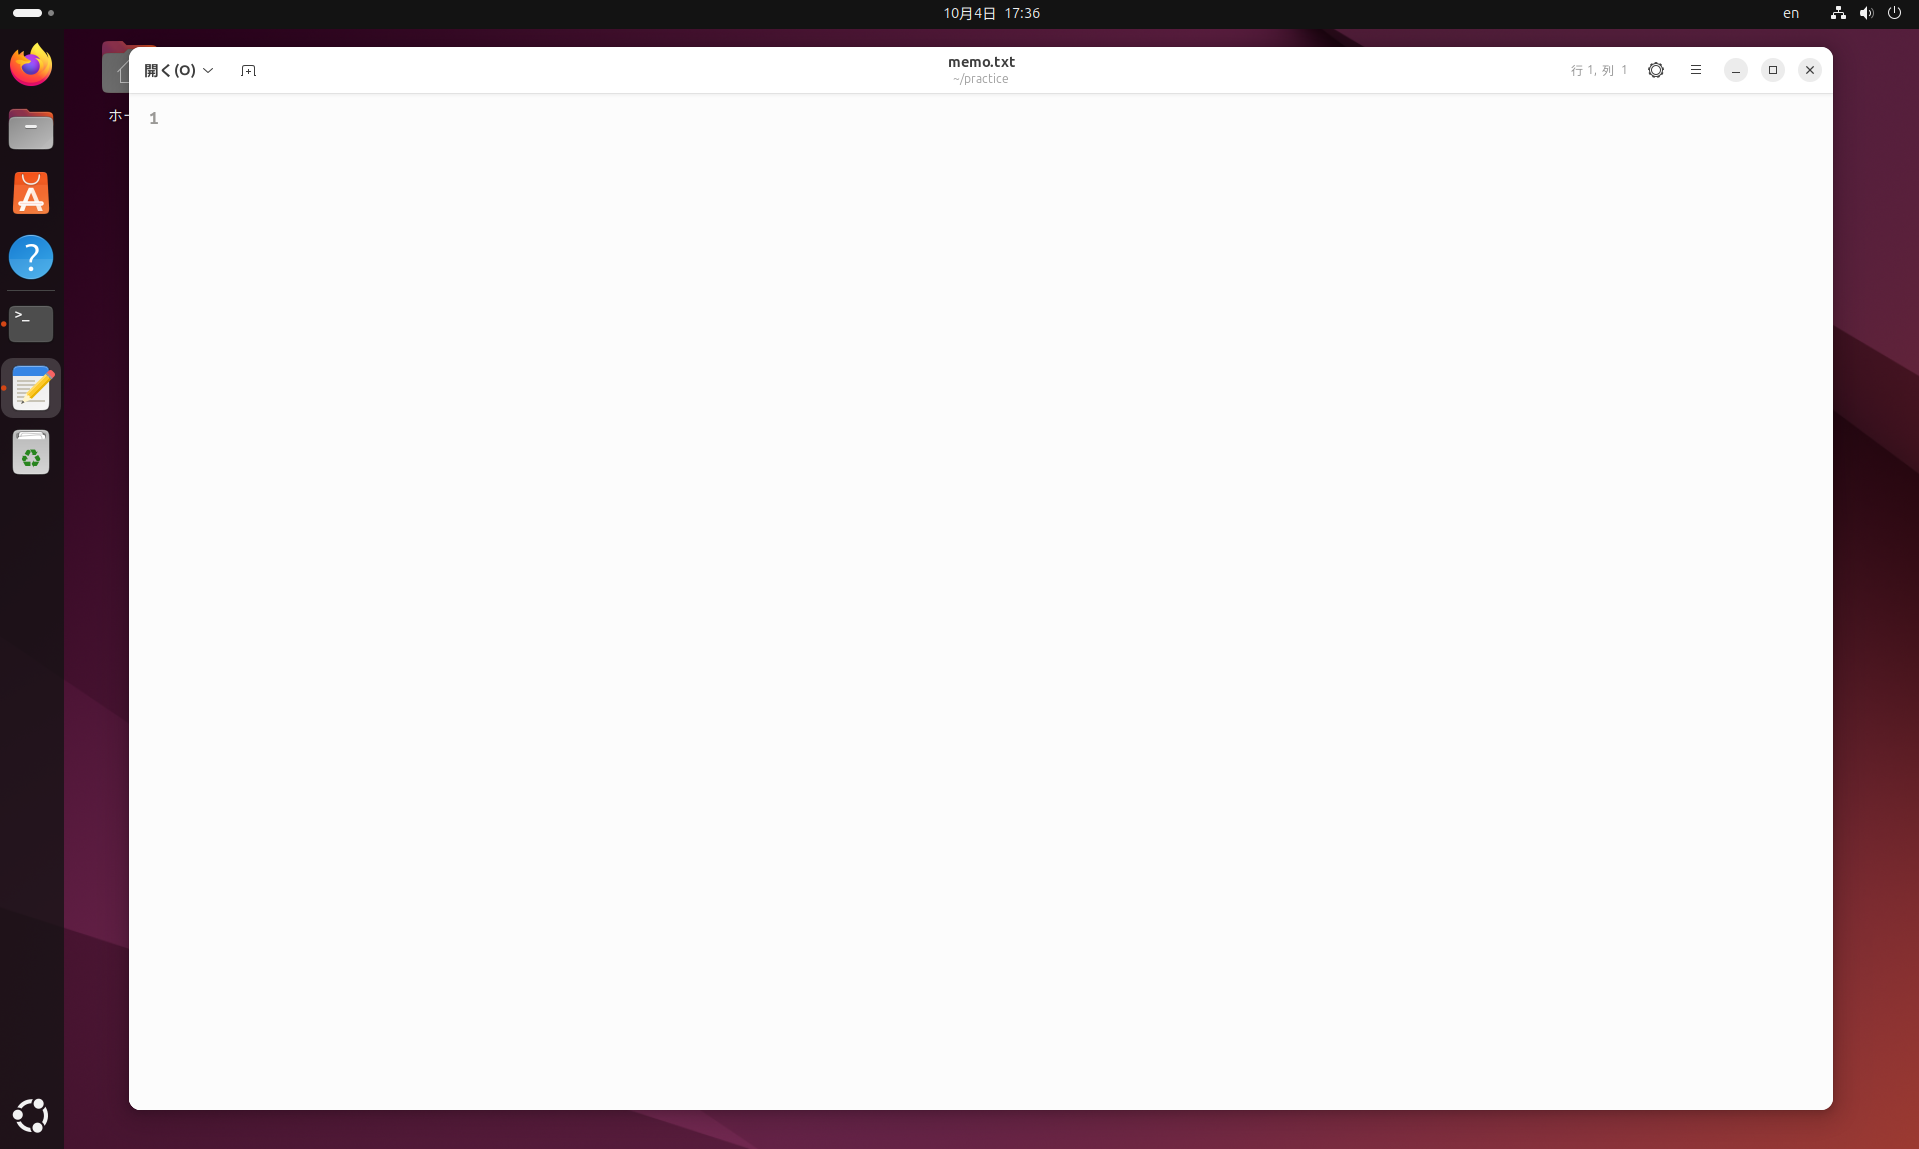
\includegraphics[width=0.9\linewidth]{files/text_editor.png}
  \caption{Ubuntu のテキストエディター}
  \label{fig:files-text-editor}
\end{figure}

\subsection{基本の操作}

テキストエディターでは、ふつうのアプリケーションと同じように、マウスでカーソルを動かしてキーボードから文字を入力できます。
よく使うキー操作は次のとおりです。

\begin{tablebox}[テキストエディターのよく使うキー操作][tab:files-editor-keys]
  \begin{tabular}{ll}
    \toprule
    キー & 動作 \\
    \midrule
    \key{Ctrl}+\key{S} & 保存する \\
    \key{Ctrl}+\key{Shift}+\key{S} & 名前を付けて保存する \\
    \key{Ctrl}+\key{O} & ファイルを開く \\
    \key{Ctrl}+\key{N} & 新しいファイルを作る（新しいタブが開く） \\
    \key{Ctrl}+\key{F} & 文字列を検索する \\
    \key{Ctrl}+\key{H} & 文字列を置換する \\
    \key{Ctrl}+\key{Z} & 元に戻す \\
    \key{Ctrl}+\key{W} & 今のタブを閉じる \\
    \bottomrule
  \end{tabular}
\end{tablebox}

保存していない変更があるときは、ウィンドウの上部のファイル名の横に印が付きます。
編集したら、こまめに \key{Ctrl}+\key{S} で保存する習慣をつけましょう。
保存すれば、ターミナルで \cmd{cat memo.txt} を実行して、書いた内容を確かめられます。

\subsection{プログラムを書くための設定}

テキストエディターの右上のメニューボタンから「設定」を開くと、表示や編集の方法を変えられます。
プログラムや設定ファイルを書くときは、次の設定をしておくと便利です。

\begin{itemize}
  \item \textbf{行番号を表示する}：エラーメッセージに「〇行目」と書かれていたときに、すぐにその行を探せます。
  \item \textbf{インデントにスペースを使う}：タブ文字の代わりに半角スペースでインデントするようにし、幅を 4 にします。Python のプログラム（第IV部）を書くときに役立ちます。
\end{itemize}

\cmd{.py} や \cmd{.sh} などの拡張子のファイルを開くと、プログラムの文法に合わせて文字に色が付きます（シンタックスハイライト）。

\subsection{隠しファイルやシステムのファイルを編集する}

\cmd{\textasciitilde/.bashrc}（\ref{chap:env}章）のような隠しファイルも、ターミナルからファイル名を指定すれば、ほかのファイルと同じように開けます。

\begin{terminal}[隠しファイルをテキストエディターで開く]
~/practice$ gnome-text-editor ~/.bashrc
\end{terminal}

一方、\cmd{/etc} の下の設定ファイルのように、root しか書き込めないファイルは、テキストエディターで開いても保存できません。
そのようなファイルを作るときは、まずホームディレクトリの中でファイルを作って保存し、それを \cmd{sudo cp}（\ref{chap:permission}章）でコピーする方法が安全です。

\begin{caution}[ワープロでプログラムを書かない]
  Word などの文書作成ソフト（ワープロ）は、文字のほかに、文字の大きさや色といった情報も一緒に保存します。
  そのため、プログラムや設定ファイルを書くのには使えません。
  プログラムや設定ファイルは、必ずテキストエディターのようなエディタで書きましょう。
\end{caution}

\begin{point}[ターミナルに戻ってこないとき]
  ターミナルから \cmd{gnome-text-editor} を起動すると、テキストエディターを閉じるまで、ターミナルが次のコマンドを受け付けなくなることがあります。
  そのときは、編集が終わったらテキストエディターを閉じるか、別のターミナルを開いて作業を続けましょう。
  \cmd{gnome-text-editor memo.txt \&} のように最後に \cmd{\&} を付けると、テキストエディターを開いたまま、ターミナルで作業を続けられます（\ref{sec:process-job}節）。
\end{point}

\section{ファイルを探す}
\label{sec:files-find}

「あのファイルはどこに置いたっけ？」というときや、「ROS 2 のあの設定ファイルはどこにあるのだろう？」というときには、ファイルを検索するコマンドを使います。

\subsection{\cmd{find}：条件を指定して探す}

\cmd{find} は、指定したディレクトリの中を下の階層までたどって、条件に合うファイルを探すコマンドです。
\cmd{find 探す場所 条件} の順に指定します。
最もよく使う条件は、名前で探す \cmd{-name} です。

\begin{terminal}[名前でファイルを探す]
~/practice$ find ~ -name memo.txt
/home/user/practice/memo.txt
/home/user/practice/a/memo.txt
\end{terminal}

\ref{sec:files-manipulate}節で \cmd{a} の中にコピーした \cmd{memo.txt} と、\ref{sec:files-edit}節でテキストエディターで作った \cmd{memo.txt} が見つかります（テキストエディターで保存していなければ、1 つ目は表示されません）。

名前の一部しかわからないときは、次の節で説明するワイルドカード \cmd{*} を使います。
このとき、パターンはクォートで囲んでください（理由は次の節で説明します）。

\begin{terminal}[名前の一部で探す]
~/practice$ find /usr/share/applications -name "org.gnome.*"
/usr/share/applications/org.gnome.TextEditor.desktop
/usr/share/applications/org.gnome.Terminal.desktop
...
\end{terminal}

\cmd{/usr/share/applications} には、アクティビティ画面に表示されるアプリケーションの情報が入っています。
表示される順番や数は、環境によって変わります。

\cmd{find} では、ほかにも次のような条件を指定できます。

\begin{tablebox}[\cmd{find} で指定できる主な条件][tab:files-find-conditions]
  \begin{tabular}{ll}
    \toprule
    条件 & 意味 \\
    \midrule
    \cmd{-name パターン} & 名前がパターンに一致する \\
    \cmd{-iname パターン} & 大文字・小文字を区別せずに名前で探す \\
    \cmd{-type f} & 通常のファイルだけを探す \\
    \cmd{-type d} & ディレクトリだけを探す \\
    \bottomrule
  \end{tabular}
\end{tablebox}

ここまでの作業で、\cmd{\textasciitilde/practice} の中には、\cmd{mkdir -p} で作った \cmd{a/b/c} が残っています。
ディレクトリだけを探してみましょう。

\begin{terminal}[ディレクトリだけを探す]
~/practice$ find ~/practice -type d
/home/user/practice
/home/user/practice/a
/home/user/practice/a/b
/home/user/practice/a/b/c
\end{terminal}

システム全体（\cmd{/}）から探すと、権限のないディレクトリについて \cmd{Permission denied} というメッセージがたくさん表示されます。
これは読めないディレクトリを飛ばしたという意味で、検索自体は続いています。

\subsection{\cmd{locate}：データベースから高速に探す}

\cmd{find} は実際にディレクトリをたどって探すので、範囲が広いと時間がかかります。
\cmd{locate} は、あらかじめ作っておいたファイル名のデータベースから探すので、システム全体からでも一瞬で見つけられます。
Ubuntu 24.04 では標準でインストールされていないので、次のように \cmd{plocate} パッケージをインストールして使います（\cmd{sudo apt install} はソフトウェアをインストールするコマンドで、\ref{chap:package}章で詳しく説明します）。

\begin{terminal}[locate を使う]
~/practice$ sudo apt install plocate
~/practice$ locate os-release
/etc/os-release
/usr/lib/os-release
...
\end{terminal}

データベースは 1 日に 1 回自動で更新されるため、作ったばかりのファイルは見つからないことがあります。
すぐに探したいときは、\cmd{sudo updatedb} を実行してデータベースを更新してください。

\section{ワイルドカードとブレース展開}
\label{sec:files-wildcard}

たくさんのファイルをまとめて操作したいとき、ファイル名を 1 つずつ入力するのは大変です。
シェルには、複数のファイル名を短く指定するためのしくみがあります。

\subsection{ワイルドカード}

\textbf{ワイルドカード}は、ファイル名のパターンを表す特別な記号です。

\begin{tablebox}[ワイルドカード][tab:files-wildcard]
  \begin{tabular}{ll}
    \toprule
    記号 & 意味 \\
    \midrule
    \cmd{*} & 任意の 0 文字以上の文字列 \\
    \cmd{?} & 任意の 1 文字 \\
    \cmd{[abc]} & \cmd{a}, \cmd{b}, \cmd{c} のどれか 1 文字 \\
    \cmd{[0-9]} & \cmd{0} から \cmd{9} までのどれか 1 文字 \\
    \bottomrule
  \end{tabular}
\end{tablebox}

練習用のファイルを作って試してみましょう。

\begin{terminal}[ワイルドカードを使う]
~/practice$ touch data1.csv data2.csv data10.csv note.txt image.png
~/practice$ ls *.csv
data1.csv  data10.csv  data2.csv
~/practice$ ls data?.csv
data1.csv  data2.csv
~/practice$ ls data[12].csv
data1.csv  data2.csv
\end{terminal}

\cmd{*.csv} は「\cmd{.csv} で終わるすべてのファイル」、\cmd{data?.csv} は「\cmd{data} と \cmd{.csv} の間がちょうど 1 文字のファイル」を表します。
ワイルドカードは \cmd{ls} だけでなく、\cmd{cp} や \cmd{mv}、\cmd{rm} など、ファイル名を受け取るどのコマンドでも使えます。

\begin{terminal}[CSV ファイルをまとめて移動する]
~/practice$ mkdir csv
~/practice$ mv *.csv csv/
~/practice$ ls csv
data1.csv  data10.csv  data2.csv
\end{terminal}

\subsection{ワイルドカードを展開するのはシェル}

ワイルドカードを解釈しているのは、実は \cmd{ls} や \cmd{mv} ではなく\textbf{シェル}です。
シェルは、コマンドを実行する前にワイルドカードを一致するファイル名の一覧に置き換え（\textbf{展開}し）てから、コマンドに渡しています。
\cmd{echo} を使うと、展開された結果を確認できます。

\begin{terminal}[ワイルドカードの展開結果を確認する]
~/practice$ echo csv/*
csv/data1.csv csv/data10.csv csv/data2.csv
\end{terminal}

つまり \cmd{mv *.csv csv/} は、シェルによって \cmd{mv data1.csv data10.csv data2.csv csv/} に書き換えられてから実行されていたのです。
\ref{sec:files-find}節の \cmd{find} でパターンをクォートで囲んだのは、シェルに展開させずに、\cmd{*} をそのまま \cmd{find} に渡すためです。

\begin{caution}[rm とワイルドカード]
  \cmd{rm *} はカレントディレクトリのファイルをすべて削除します。
  \cmd{rm *.txt} のつもりで \cmd{rm * .txt} と余計なスペースを入れてしまうと、すべてのファイルが消えてしまいます。
  ワイルドカードを使って削除する前に、同じパターンで \cmd{ls} や \cmd{echo} を実行し、対象のファイルを確認する習慣をつけましょう。
\end{caution}

\subsection{ブレース展開}

\textbf{ブレース展開}は、\cmd{\{ \}} の中にカンマ区切りで書いた文字列を、それぞれ展開するしくみです。
ワイルドカードと違って、ファイルが存在するかどうかに関係なく展開されるので、新しくファイルやディレクトリを作るときにも使えます。

\begin{terminal}[ブレース展開]
~/practice$ echo file_{a,b,c}.txt
file_a.txt file_b.txt file_c.txt
~/practice$ echo log{1..5}
log1 log2 log3 log4 log5
\end{terminal}

\cmd{\{1..5\}} のように \cmd{..} でつなぐと、連続した数字や文字に展開されます。
ブレース展開を使うと、複数のディレクトリを一度に作ることができます。

\begin{terminal}[複数のディレクトリを一度に作る]
~/practice$ mkdir -p my_robot/{config,launch,scripts}
~/practice$ ls my_robot
config  launch  scripts
\end{terminal}

ファイルのバックアップを作るときにも便利です。

\begin{terminal}[バックアップを作る]
~/practice$ cp note.txt{,.bak}
~/practice$ ls note*
note.txt  note.txt.bak
\end{terminal}

\cmd{note.txt\{,.bak\}} は \cmd{note.txt note.txt.bak} に展開されるので、\cmd{cp note.txt note.txt.bak} と入力したのと同じ意味になります。

練習用のディレクトリ \cmd{\textasciitilde/practice} は、次の章からも使うので、削除せずに残しておきましょう。

\section*{この章のまとめ}

\begin{itemize}
  \item \cmd{pwd} でカレントディレクトリを確認し、\cmd{ls} で中身を表示し、\cmd{cd} で移動します。
  \item パスには、\cmd{/} から始まる絶対パスと、カレントディレクトリを起点とする相対パスがあります。\cmd{\textasciitilde} はホームディレクトリ、\cmd{.} はカレントディレクトリ、\cmd{..} は親ディレクトリを表します。
  \item \cmd{mkdir}, \cmd{touch}, \cmd{cp}, \cmd{mv}, \cmd{rm} で、ファイルやディレクトリを作成・コピー・移動・削除します。\cmd{rm} で消したファイルは元に戻せません。
  \item \cmd{cat}, \cmd{less}, \cmd{head}, \cmd{tail} でファイルの中身を確認します。
  \item ファイルの中身は、Ubuntu に最初から入っている「テキストエディター」で編集できます。ターミナルからは \cmd{gnome-text-editor ファイル名} で起動します。
  \item \cmd{find} や \cmd{locate} でファイルを探します。
  \item ワイルドカードとブレース展開はシェルが展開するしくみで、複数のファイルをまとめて指定できます。
\end{itemize}

\begin{tablebox}[この章で学んだコマンド][tab:files-commands]
  \begin{tabular}{ll}
    \toprule
    コマンド & 働き \\
    \midrule
    \cmd{pwd} & カレントディレクトリを表示する \\
    \cmd{ls} & ディレクトリの中身を表示する \\
    \cmd{cd} & ディレクトリを移動する \\
    \cmd{mkdir} & ディレクトリを作る \\
    \cmd{touch} & 空のファイルを作る \\
    \cmd{cp} & コピーする \\
    \cmd{mv} & 移動する・名前を変える \\
    \cmd{rm} & 削除する \\
    \cmd{cat} & ファイルの中身を表示する \\
    \cmd{less} & ファイルを 1 画面ずつ表示する \\
    \cmd{head} / \cmd{tail} & ファイルの先頭 / 末尾を表示する \\
    \cmd{find} / \cmd{locate} & ファイルを探す \\
    \bottomrule
  \end{tabular}
\end{tablebox}

\chapter{パーミッションとユーザ管理}
\label{chap:permission}

% この章で学ぶこと
\begin{goalbox}
  \begin{itemize}
    \item \cmd{ls -l} で表示されるパーミッション（権限）の読み方
    \item \cmd{chmod} と \cmd{chown} を使った権限と所有者の変更
    \item \cmd{sudo} を安全に使うための考え方
    \item センサやマイコンなどのデバイスを使うための権限の設定
  \end{itemize}
\end{goalbox}

\ref{sec:linux-internals-users}節で学んだように、Linux のすべてのファイルには所有者がいて、誰がそのファイルを読んだり書いたりできるかが決められています。
この「誰が何をしてよいか」の設定を\textbf{パーミッション}（権限）といいます。
「\cmd{Permission denied}（権限がありません）」というエラーは、ロボット開発で最もよく目にするエラーの 1 つです。
この章では、パーミッションのしくみを理解し、このエラーに自分で対処できるようになりましょう。

\section{パーミッションの読み方}
\label{sec:permission-read}

\subsection{\cmd{ls -l} の表示}

ファイルのパーミッションは、\cmd{ls -l}（\ref{sec:files-navigation}節）で確認できます。
この章では、\ref{chap:files}章で作った \cmd{\textasciitilde/practice} の中に、練習用のディレクトリ \cmd{perm} を作って試します。

\begin{terminal}[練習用のファイルを作って、パーミッションを確認する]
$ mkdir ~/practice/perm
$ cd ~/practice/perm
$ mkdir scripts
$ touch notes.txt start_robot.sh
$ ls -l
total 4
-rw-rw-r-- 1 user user    0 Sep 30 10:01 notes.txt
drwxrwxr-x 2 user user 4096 Sep 30 10:00 scripts
-rw-rw-r-- 1 user user    0 Sep 30 10:02 start_robot.sh
\end{terminal}

左端の 10 文字がパーミッションで、3 列目と 4 列目がそれぞれ所有者とグループです（日時やファイルの大きさは、環境によって変わります）。
10 文字は、図\ref{fig:permission-string}のように区切って読みます。

\begin{figure}[tb]
  \centering
  % 図：パーミッションの表記の読み方（chapters/commandline/permission.tex）
\begin{tikzpicture}[ch/.style={font=\Large\ttfamily, inner sep=0pt, outer sep=0pt, anchor=base west, minimum width=5mm}]
  \foreach \c [count=\i from 0] in {-,r,w,x,r,-,x,r,-,-}
    \node[ch] (c\i) at (\i*0.5,0) {\c};
  % 区切りの色
  \begin{scope}[on background layer]
    \fill[black!10] ([yshift=-1mm]c0.south west) rectangle ([yshift=5mm]c0.south east);
    \fill[blue!15] ([yshift=-1mm]c1.south west) rectangle ([yshift=5mm]c3.south east);
    \fill[green!15] ([yshift=-1mm]c4.south west) rectangle ([yshift=5mm]c6.south east);
    \fill[orange!15] ([yshift=-1mm]c7.south west) rectangle ([yshift=5mm]c9.south east);
  \end{scope}
  \node[figlabel, below=3mm of c0] {種類};
  \node[figlabel, below=3mm of c2, align=center] {所有者\\（user）};
  \node[figlabel, below=3mm of c5, align=center] {グループ\\（group）};
  \node[figlabel, below=3mm of c8, align=center] {その他\\（others）};
  % 右側の説明
  \node[figlabel, anchor=west, align=left] at (5.6,-0.2)
    {\texttt{-}：通常のファイル　\texttt{d}：ディレクトリ\\
     \texttt{r}：読み取り（read）\\
     \texttt{w}：書き込み（write）\\
     \texttt{x}：実行（execute）\\
     \texttt{-}：その権限がない};
\end{tikzpicture}

  \caption{パーミッションの表記の読み方（\cmd{-rwxr-xr--} の場合）}
  \label{fig:permission-string}
\end{figure}

\begin{enumerate}
  \item 1 文字目はファイルの種類です。\cmd{-} は通常のファイル、\cmd{d} はディレクトリ、\cmd{l} はシンボリックリンク、\cmd{c} はデバイスファイル（\ref{sec:linux-internals-device}節）を表します。
  \item 2〜4 文字目は、\textbf{所有者}（user）に対する権限です。
  \item 5〜7 文字目は、ファイルに設定された\textbf{グループ}（group）のメンバーに対する権限です。
  \item 8〜10 文字目は、それ以外のすべてのユーザ（\textbf{その他}、others）に対する権限です。
\end{enumerate}

それぞれの 3 文字は、左から順に「読み取り（\cmd{r}）」「書き込み（\cmd{w}）」「実行（\cmd{x}）」ができるかどうかを表し、できない場合は \cmd{-} になります。
今作った \cmd{notes.txt} の \cmd{-rw-rw-r--} は、所有者とグループのメンバーが読み書きでき、その他のユーザは読み取りだけができる、という意味です。
図\ref{fig:permission-string}の \cmd{-rwxr-xr--} なら、次の意味になります（次の節で、\cmd{start\_robot.sh} をこの権限に変えてみます）。

\begin{itemize}
  \item 所有者の \cmd{user} は、読み取り・書き込み・実行のすべてができる（\cmd{rwx}）
  \item グループ \cmd{user} のメンバーは、読み取りと実行ができる（\cmd{r-x}）
  \item その他のユーザは、読み取りだけができる（\cmd{r--}）
\end{itemize}

\subsection{ファイルとディレクトリでの意味の違い}

\cmd{r}, \cmd{w}, \cmd{x} の意味は、ファイルとディレクトリで少し異なります。

\begin{tablebox}[ファイルとディレクトリでの権限の意味][tab:permission-rwx]
  \begin{tabular}{lp{0.35\linewidth}p{0.35\linewidth}}
    \toprule
    権限 & ファイルの場合 & ディレクトリの場合 \\
    \midrule
    \cmd{r} & 中身を読める & 中のファイルの一覧を見られる \\
    \cmd{w} & 中身を書き換えられる & 中にファイルを作ったり、削除したりできる \\
    \cmd{x} & プログラムとして実行できる & \cmd{cd} で中に入れる \\
    \bottomrule
  \end{tabular}
\end{tablebox}

シェルスクリプト（\ref{chap:shellscript}章）や Python のスクリプト（\ref{sec:python-run}節）を \cmd{./start\_robot.sh} のように直接実行するには、ファイルに \cmd{x} の権限が必要です。
権限がないと、次のようなエラーになります。

\begin{terminal}[実行権限がないファイルを実行した場合]
$ ./notes.txt
bash: ./notes.txt: Permission denied
\end{terminal}

\section{chmod, chown の使い方}
\label{sec:permission-chmod}

\subsection{\cmd{chmod}：権限を変える}

ファイルの権限を変えるには、\cmd{chmod}（change mode）を使います。
権限の指定の仕方には、記号で書く方法と数字で書く方法があります。

\textbf{記号で指定する方法}では、「誰に（\cmd{u}：所有者、\cmd{g}：グループ、\cmd{o}：その他、\cmd{a}：全員）」「追加するか削除するか（\cmd{+} / \cmd{-}）」「どの権限を（\cmd{r}, \cmd{w}, \cmd{x}）」を組み合わせて書きます。

\begin{terminal}[記号で権限を変える]
$ chmod u+x start_robot.sh      # 所有者に実行権限を追加
$ chmod go-w notes.txt          # グループとその他から書き込み権限を削除
$ chmod +x start_robot.sh       # 誰にも指定しないと、全員に追加
\end{terminal}

最もよく使うのは、スクリプトに実行権限を付ける \cmd{chmod +x} です。

\textbf{数字で指定する方法}では、\cmd{r} を 4、\cmd{w} を 2、\cmd{x} を 1 として、所有者・グループ・その他のそれぞれについて足し算した数字を 3 桁並べて書きます。

\begin{tablebox}[\cmd{chmod} の数字による指定の例][tab:permission-numeric]
  \begin{tabular}{llll}
    \toprule
    数字 & 表記 & 意味 & よく使う場面 \\
    \midrule
    \cmd{755} & \cmd{rwxr-xr-x} & 所有者はすべて、ほかは読み取りと実行 & スクリプト、ディレクトリ \\
    \cmd{644} & \cmd{rw-r--r--} & 所有者は読み書き、ほかは読み取りだけ & 通常のファイル \\
    \cmd{700} & \cmd{rwx------} & 所有者だけがすべてできる & 自分専用のディレクトリ \\
    \cmd{600} & \cmd{rw-------} & 所有者だけが読み書きできる & 秘密鍵など \\
    \bottomrule
  \end{tabular}
\end{tablebox}

\begin{terminal}[数字で権限を変える]
$ chmod 754 start_robot.sh
$ ls -l start_robot.sh
-rwxr-xr-- 1 user user 0 Sep 30 10:02 start_robot.sh
$ chmod 755 start_robot.sh
$ ls -l start_robot.sh
-rwxr-xr-x 1 user user 0 Sep 30 10:02 start_robot.sh
\end{terminal}

たとえば \cmd{755} は、所有者が $4+2+1=7$、グループが $4+1=5$、その他が $4+1=5$ という意味です。
\cmd{754} なら、その他が $4$（読み取りだけ）になり、図\ref{fig:permission-string}と同じ \cmd{-rwxr-xr--} になります。

\begin{caution}[\cmd{chmod 777} は使わない]
  「\cmd{Permission denied} が出たら \cmd{chmod 777} すればよい」という情報をインターネットで見かけることがあります。
  \cmd{777} は、誰でも読み書き・実行ができるという設定で、ほかのユーザや悪意のあるプログラムに書き換えられる危険があります。
  エラーが出たら、まずは \cmd{ls -l} で「誰に」「どの権限が」足りないのかを確かめて、必要な権限だけを追加しましょう。
\end{caution}

\subsection{\cmd{chown}：所有者を変える}

ファイルの所有者やグループを変えるには、\cmd{chown}（change owner）を使います。
所有者を変えられるのは root だけなので、\cmd{sudo} を付けて実行します。
\cmd{所有者:グループ} のように書くと、両方を同時に変えられます。
ディレクトリの中身もまとめて変えるときは \cmd{-R} を付けます。

うっかり \cmd{sudo} を付けて作ったファイルは、所有者が root になり、自分では編集できなくなります（\ref{sec:linux-internals-users}節）。
そのようなときに、\cmd{chown} で所有者を自分に戻します。
\cmd{sudo} を付けてファイルを作り、所有者を戻してみましょう。

\begin{terminal}[所有者を変える]
$ sudo touch root_file.txt
$ ls -l root_file.txt
-rw-r--r-- 1 root root 0 Sep 30 10:05 root_file.txt
$ sudo chown user:user root_file.txt
$ ls -l root_file.txt
-rw-r--r-- 1 user user 0 Sep 30 10:05 root_file.txt
\end{terminal}

\cmd{user:user} の部分は、自分のユーザ名に置き換えてください（\cmd{\$USER:\$USER} と書くこともできます。\cmd{\$USER} については\ref{chap:env}章で説明します）。
ディレクトリを中身ごと変えるときは、\cmd{sudo chown -R user:user ディレクトリ名} のように \cmd{-R} を付けます。

\section{sudo と安全な権限の扱い方}
\label{sec:permission-sudo}

\subsection{\cmd{sudo} のしくみ}

\ref{sec:linux-internals-users}節で説明したように、\cmd{sudo} は、後ろに書いたコマンドを root の権限で実行するためのコマンドです。
\cmd{sudo} を使えるのは \cmd{sudo} グループのメンバーだけで、どのユーザがどのコマンドを実行できるかは \cmd{/etc/sudoers} というファイルで決められています。
一度パスワードを入力すると、しばらく（標準では 15 分）はパスワードを聞かれずに \cmd{sudo} を使えます。

\subsection{\cmd{sudo} を使うべきとき・使うべきでないとき}

\cmd{sudo} が必要になるのは、主にシステム全体に関わる操作をするときです。

\begin{itemize}
  \item ソフトウェアのインストールや更新（\cmd{sudo apt install} など、\ref{chap:package}章）
  \item \cmd{/etc} の下の設定ファイルの編集
  \item ほかのユーザが所有するファイルの操作
\end{itemize}

逆に、自分のホームディレクトリの中での作業には、\cmd{sudo} は必要ありません。
ROS 2 のワークスペースのビルド（\ref{chap:workspace}章）や、自分のプログラムの実行、Python のパッケージのインストール（\ref{chap:python_env}章）に \cmd{sudo} を付けると、root が所有するファイルができてしまい、後でトラブルの原因になります。

\begin{point}[\cmd{Permission denied} が出たときの考え方]
  \begin{enumerate}
    \item エラーの出たファイルやディレクトリを \cmd{ls -l} で確認し、所有者・グループ・権限を見る
    \item 自分のファイルなのに権限が足りないなら、\cmd{chmod} で必要な権限を追加する
    \item 所有者が root になってしまっているなら、\cmd{sudo chown} で自分に戻す
    \item システムの設定を変える操作なら、\cmd{sudo} を付けて実行する
  \end{enumerate}
  「とりあえず \cmd{sudo} を付ける」のは、根本的な解決にならないことが多いので避けましょう。
\end{point}

\subsection{\cmd{sudo} とリダイレクト}

\cmd{sudo} を使っても、うまくいかない書き方があります。
たとえば、root しか書き込めないファイルに、\cmd{>}（\ref{sec:text-pipe-redirect}節）で文字を書き込もうとすると、\cmd{sudo} を付けてもエラーになります。

\begin{terminal}[sudo を付けても書き込めない例]
$ sudo echo "hello" > /etc/robot.conf
bash: /etc/robot.conf: Permission denied
\end{terminal}

これは、\cmd{sudo} が root の権限で実行するのは \cmd{echo} だけで、ファイルへの書き込み（\cmd{>}）は、一般ユーザの権限のシェルが行っているためです。
このような場合は、\cmd{tee} コマンドを \cmd{sudo} で実行して書き込みます。

\begin{terminal}[tee を使って root の権限で書き込む]
$ echo "hello" | sudo tee /etc/robot.conf
hello
\end{terminal}

\cmd{tee} は、受け取った文字を画面に表示しながらファイルにも書き込むコマンドです（\ref{sec:text-pipe-pipe}節）。
Docker のリポジトリを登録するとき（\ref{sec:docker-basic}節）にも、この書き方が使われています。

\section{デバイスへのアクセス権}
\label{sec:permission-device}

\subsection{デバイスファイルの権限}

USB でつないだセンサやマイコンを使おうとして、\cmd{Permission denied} というエラーが出ることがあります。
デバイスファイル（\ref{sec:linux-internals-device}節）のパーミッションを見てみましょう。
次は、USB シリアルの機器（マイコンボードなど）をつないだときの例です。
機器をつないでいなければ \cmd{/dev/ttyUSB0} はないので、同じ結果にはなりません。

\begin{termexample}[デバイスファイルの権限を確認する]
$ ls -l /dev/ttyUSB0
crw-rw---- 1 root dialout 188, 0 Sep 30 10:15 /dev/ttyUSB0
\end{termexample}

1 文字目の \cmd{c} は、デバイスファイル（キャラクタデバイス）であることを表しています。
所有者は root、グループは \cmd{dialout} で、所有者とグループのメンバーだけが読み書きできる（\cmd{rw-rw----}）ことがわかります。
つまり、このデバイスを使うには、自分が \cmd{dialout} グループのメンバーである必要があります。

\subsection{グループにユーザを追加する}

自分が所属しているグループは、\cmd{groups} コマンドで確認できます。

\begin{terminal}[所属しているグループを確認する]
$ groups
user adm cdrom sudo dip plugdev users lpadmin
\end{terminal}

\cmd{dialout} が含まれていなければ、\cmd{usermod} コマンドで自分を \cmd{dialout} グループに追加します。
\cmd{-aG} は、「今のグループに加えて（append）、このグループ（Group）にも所属させる」という意味です。
\cmd{\$USER} は、自分のユーザ名が入った環境変数です（\ref{chap:env}章）。

\begin{terminal}[dialout グループに自分を追加する]
$ sudo usermod -aG dialout $USER
\end{terminal}

\textbf{グループの変更は、一度ログアウトしてログインし直すまで反映されません。}
再ログインしてから \cmd{groups} を実行し、\cmd{dialout} が含まれていることを確かめましょう。

\begin{caution}[\cmd{-a} を忘れない]
  \cmd{usermod -G dialout} のように \cmd{-a} を付け忘れると、今まで所属していたグループ（\cmd{sudo} など）から外れて、\cmd{dialout} だけに所属することになってしまいます。
  \cmd{sudo} グループから外れると \cmd{sudo} が使えなくなるので、必ず \cmd{-aG} と書きましょう。
\end{caution}

ロボット開発では、\cmd{dialout} のほかに、次のようなグループがよく出てきます。

\begin{tablebox}[ロボット開発でよく出てくるグループ][tab:permission-groups]
  \begin{tabular}{lp{0.6\linewidth}}
    \toprule
    グループ & 使えるようになるもの \\
    \midrule
    \cmd{dialout} & USB シリアルの機器（\cmd{/dev/ttyUSB0}, \cmd{/dev/ttyACM0}） \\
    \cmd{video} & カメラ（\cmd{/dev/video0}） \\
    \cmd{input} & ゲームパッドなどの入力機器（\cmd{/dev/input/}） \\
    \cmd{docker} & \cmd{sudo} なしでの \cmd{docker} コマンド（\ref{chap:docker}章） \\
    \bottomrule
  \end{tabular}
\end{tablebox}

\begin{column}{udev でデバイスの設定を固定する}
  \cmd{sudo chmod 666 /dev/ttyUSB0} のようにデバイスファイルの権限を直接変えても、機器を挿し直したり再起動したりすると元に戻ってしまいます。
  また、デバイスファイルの番号は、つないだ順番で変わってしまいます（\ref{sec:linux-internals-device}節）。
  実際のロボットでは、\textbf{udev} というしくみを使って、これらを解決することがよくあります。
  udev は、機器がつながったときに、デバイスファイルの名前や権限を決めるしくみです。
  \cmd{/etc/udev/rules.d/} の下に\textbf{ルール}を書いたファイルを置いておくと、たとえば「この LiDAR がつながったら、いつでも \cmd{/dev/lidar} という名前を付け、誰でも使える権限にする」といった設定ができます。
  センサのメーカーが、udev のルールファイルを用意してくれていることも多いので、機器の説明書を確認してみましょう。
\end{column}

\section*{この章のまとめ}

\begin{itemize}
  \item パーミッションは、所有者・グループ・その他のそれぞれに対して、読み取り（\cmd{r}）・書き込み（\cmd{w}）・実行（\cmd{x}）ができるかを表します。\cmd{ls -l} で確認できます。
  \item \cmd{chmod} で権限を、\cmd{sudo chown} で所有者を変えます。スクリプトには \cmd{chmod +x} で実行権限を付けます。\cmd{chmod 777} は避けましょう。
  \item \cmd{sudo} はシステム全体に関わる操作のときだけ使います。\cmd{Permission denied} が出たら、まず \cmd{ls -l} で原因を確かめます。
  \item USB のセンサやマイコンを使うには、\cmd{dialout} グループに自分を追加します（反映には再ログインが必要）。
  \item udev のルールを使うと、デバイスに固定の名前と権限を設定できます。
\end{itemize}

\chapter{テキスト処理とパイプ}
\label{chap:text_pipe}

% この章で学ぶこと
\begin{goalbox}
  \begin{itemize}
    \item TODO
  \end{itemize}
\end{goalbox}

\section{標準入力・標準出力・標準エラー出力}

TODO

\section{リダイレクト}

TODO

\section{パイプでコマンドをつなぐ}

TODO

\section{検索と加工}

TODO

\section{sed と awk の入門}

TODO

\section*{この章のまとめ}

TODO

\chapter{プロセスとシステム管理}
\label{chap:process}

% この章で学ぶこと
\begin{goalbox}
  \begin{itemize}
    \item 動いているプロセスの確認（\cmd{ps}, \cmd{top}, \cmd{htop}）
    \item フォアグラウンドとバックグラウンドの切り替え（ジョブ制御）
    \item シグナルとプロセスの終了（\cmd{kill}, \cmd{pkill}）
    \item ストレージとメモリの使用量の確認（\cmd{df}, \cmd{du}, \cmd{free}）
    \item システムのログの確認（\cmd{journalctl}, \cmd{dmesg}）
  \end{itemize}
\end{goalbox}

\ref{sec:linux-internals-process}節で学んだように、実行中のプログラムはプロセスとして動いています。
ロボットを動かすときには、センサのドライバや制御のプログラムなど、たくさんのプロセスが同時に動きます。
「プログラムが止まらない」「動作が重い」「センサが認識されない」といったトラブルに対処するには、プロセスやシステムの状態を確認する方法を知っておく必要があります。

\section{プロセスの確認}
\label{sec:process-check}

\subsection{\cmd{ps}：プロセスの一覧を表示する}

\cmd{ps} は、動いているプロセスの一覧を表示するコマンドです。
引数なしで実行すると、今のターミナルで動いているプロセスだけが表示されます。

\begin{terminal}[今のターミナルのプロセスを表示する]
$ ps
    PID TTY          TIME CMD
   2345 pts/0    00:00:00 bash
   2789 pts/0    00:00:00 ps
\end{terminal}

\cmd{PID} はプロセス ID、\cmd{CMD} は実行しているコマンドです。
シェル（bash）と、今実行した \cmd{ps} 自身が表示されています。

システム全体のプロセスを表示するには、\cmd{ps aux} とします。
非常にたくさんのプロセスが表示されるので、パイプ（\ref{sec:text-pipe-pipe}節）で \cmd{grep} と組み合わせて、目的のプロセスを探すのが定番の使い方です。

\begin{terminal}[システム全体から目的のプロセスを探す]
$ ps aux | grep python3
USER         PID %CPU %MEM    VSZ   RSS TTY      STAT START   TIME COMMAND
user        4012 12.5  0.6 345680 98012 pts/1    Sl+  10:31   0:15 python3 controller.py
user        4150  0.0  0.0   9212  2304 pts/2    S+   10:33   0:00 grep --color=auto python3
\end{terminal}

\cmd{\%CPU} と \cmd{\%MEM} は、そのプロセスが使っている CPU とメモリの割合です。
最後の行は、検索に使った \cmd{grep} 自身です。

\subsection{\cmd{top} と \cmd{htop}：リアルタイムに監視する}

\cmd{top} は、プロセスの状態をリアルタイムで表示し続けるコマンドです。
CPU やメモリを多く使っているプロセスが上に表示されるので、「コンピュータが重い」ときに原因を探すのに役立ちます。

\begin{terminal}[プロセスをリアルタイムで監視する]
$ top
top - 10:35:01 up  2:15,  1 user,  load average: 0.52, 0.48, 0.41
Tasks: 312 total,   1 running, 311 sleeping,   0 stopped,   0 zombie
%Cpu(s):  3.1 us,  1.0 sy,  0.0 ni, 95.6 id,  0.2 wa,  0.0 hi,  0.1 si,  0.0 st
MiB Mem :  15890.2 total,   9012.3 free,   3456.7 used,   3421.2 buff/cache
MiB Swap:   4096.0 total,   4096.0 free,      0.0 used.  12433.5 avail Mem

    PID USER      PR  NI    VIRT    RES    SHR S  %CPU  %MEM     TIME+ COMMAND
   4012 user      20   0  345680  98012  21504 S  12.5   0.6   0:15.23 python3
   1523 user      20   0 4812344 412300 150212 S   4.3   2.5   2:01.87 gnome-shell
...
\end{terminal}

\cmd{top} を実行している間は、次のキーで操作できます。
\key{P} で CPU の使用率の順に、\key{M} でメモリの使用量の順に並べ替え、\key{1} で CPU のコアごとの使用率を表示し、\key{q} で終了します。

\cmd{htop} は、\cmd{top} をより見やすく、使いやすくしたコマンドです。
CPU のコアごとの使用率やメモリの使用量がグラフで表示され、矢印キーでプロセスを選んで操作できます。
標準では入っていないので、インストールして使います（\ref{chap:package}章）。

\begin{terminal}[htop をインストールして起動する]
$ sudo apt install htop
$ htop
\end{terminal}

\begin{column}{load average}
  \cmd{top} の 1 行目の \cmd{load average} は、CPU の使用を待っているプロセスの数の平均で、左から直近 1 分・5 分・15 分の値です。
  CPU のコアの数（\cmd{nproc} で確認できます）と比べて、この値がずっと大きい状態が続いているなら、コンピュータの処理能力が足りていないということです。
  ロボットの PC でこの値が高いときは、処理を軽くするか、より性能の高いコンピュータを検討しましょう。
\end{column}

\section{フォアグラウンドとバックグラウンド}
\label{sec:process-job}

\subsection{ジョブ}

ターミナルでコマンドを実行すると、ふつうはそのコマンドが終わるまで、次のコマンドを入力できません。
このように、ターミナルを占有して動いている状態を\textbf{フォアグラウンド}といいます。
これに対して、コマンドを裏で動かしたまま、ターミナルで別のコマンドを入力できる状態を\textbf{バックグラウンド}といいます。
シェルから起動したこれらのプロセスを、\textbf{ジョブ}と呼びます（図\ref{fig:process-job}）。

\begin{figure}[tb]
  \centering
  % 図：ジョブの状態の切り替え（chapters/commandline/process.tex）
\begin{tikzpicture}[
    >=Stealth, auto, node distance=26mm and 50mm, on grid,
    every state/.style={draw, rounded corners, rectangle, fill=blue!6,
      minimum width=28mm, minimum height=10mm, font=\small, align=center}]
  \node[state, fill=blue!15] (fg) {\textbf{フォアグラウンド}\\{\footnotesize 端末を占有して実行}};
  \node[state, right=of fg, fill=green!8] (bg) {\textbf{バックグラウンド}\\{\footnotesize 裏で実行}};
  \node[state, below right=26mm and 25mm of fg, fill=orange!10] (st) {\textbf{停止中}\\{\footnotesize 一時停止}};
  \path[->, thick]
    (bg) edge node[font=\footnotesize, swap]{\texttt{fg}} (fg)
    (fg) edge node[font=\footnotesize]{\texttt{Ctrl+Z}} (st)
    (st) edge[bend right=20] node[font=\footnotesize, swap]{\texttt{bg}} (bg)
    (st) edge[bend left=40] node[font=\footnotesize]{\texttt{fg}} (fg);
  \node[font=\footnotesize, anchor=south] (s1) at ([yshift=6mm]fg.north) {\texttt{コマンド}};
  \node[font=\footnotesize, anchor=south] (s2) at ([yshift=6mm]bg.north) {\texttt{コマンド \&}};
  \draw[->, thick] (s1) -- (fg);
  \draw[->, thick] (s2) -- (bg);
\end{tikzpicture}

  \caption{ジョブの状態の切り替え}
  \label{fig:process-job}
\end{figure}

\subsection{バックグラウンドで実行する}

コマンドの最後に \cmd{\&} を付けると、バックグラウンドで実行されます。
ここでは、指定した秒数だけ待つ \cmd{sleep} コマンドを使って試してみます。

\begin{terminal}[バックグラウンドで実行する]
$ sleep 100 &
[1] 3456
$ jobs
[1]+  Running                 sleep 100 &
\end{terminal}

\cmd{[1]} はジョブ番号、\cmd{3456} は PID です。
\cmd{jobs} で、今のシェルのジョブの一覧を確認できます。

\subsection{フォアグラウンドとバックグラウンドを切り替える}

\cmd{fg} で、バックグラウンドのジョブをフォアグラウンドに戻せます。
フォアグラウンドで動いているジョブは、\key{Ctrl}+\key{Z} で一時停止でき、\cmd{bg} でバックグラウンドで再開できます。
\cmd{\%1} のように書くと、ジョブ番号でジョブを指定できます。

\begin{terminal}[ジョブを切り替える]
$ fg %1
sleep 100
^Z
[1]+  Stopped                 sleep 100
$ bg %1
[1]+ sleep 100 &
\end{terminal}

\cmd{\textasciicircum Z} は、\key{Ctrl}+\key{Z} を押したことを表しています。

\begin{caution}[\key{Ctrl}+\key{Z} は終了ではない]
  \key{Ctrl}+\key{Z} は、プログラムを\textbf{一時停止}するだけで、終了はしません。
  ROS 2 のノードを止めるつもりで \key{Ctrl}+\key{Z} を押すと、ノードが止まったまま残り続け、同じ名前のノードが重複するなどのトラブルの原因になります。
  プログラムを終了するときは、\key{Ctrl}+\key{C} を使いましょう。
\end{caution}

バックグラウンドのジョブは、ターミナルを閉じると一緒に終了します。
ターミナルを閉じたり、SSH の接続が切れたりしても動かし続けたいときは、tmux（\ref{sec:network-tmux}節）を使うと便利です。

\section{プロセスの終了とシグナル}
\label{sec:process-kill}

\subsection{シグナル}

プロセスには、\textbf{シグナル}という合図を送って、終了や一時停止などを指示できます。
\key{Ctrl}+\key{C} や \key{Ctrl}+\key{Z} も、実はフォアグラウンドのプロセスにシグナルを送る操作です。
よく使うシグナルには、次のようなものがあります。

\begin{tablebox}[よく使うシグナル][tab:process-signals]
  \begin{tabular}{llp{0.5\linewidth}}
    \toprule
    シグナル & 番号 & 意味 \\
    \midrule
    \cmd{SIGINT} & 2 & 割り込み。\key{Ctrl}+\key{C} で送られる \\
    \cmd{SIGTERM} & 15 & 終了の依頼。\cmd{kill} で標準で送られる \\
    \cmd{SIGKILL} & 9 & 強制終了。プロセスは拒否できない \\
    \cmd{SIGTSTP} & 20 & 一時停止。\key{Ctrl}+\key{Z} で送られる \\
    \cmd{SIGHUP} & 1 & 端末が切断された。ターミナルを閉じると送られる \\
    \bottomrule
  \end{tabular}
\end{tablebox}

\cmd{SIGINT} や \cmd{SIGTERM} を受け取ったプログラムは、ファイルを保存したり、モータを止めたりといった後片付けをしてから終了できます。
ROS 2 のノードも、\key{Ctrl}+\key{C}（\cmd{SIGINT}）を受け取ると、きちんと終了処理を行ってから終了するように作られています。
一方、\cmd{SIGKILL} を受けたプロセスは、後片付けをする間もなく即座に終了させられます。

\subsection{\cmd{kill}：シグナルを送る}

別のターミナルで動いているプロセスや、バックグラウンドのプロセスを終了させるには、\cmd{kill} で PID を指定してシグナルを送ります。
シグナルを指定しなければ \cmd{SIGTERM} が送られます。

\begin{terminal}[プロセスを終了させる]
$ kill 4012                # SIGTERM を送る（終了を依頼する）
$ kill -INT 4012           # SIGINT を送る（Ctrl+C と同じ）
$ kill -9 4012             # SIGKILL を送る（強制終了）
\end{terminal}

\begin{point}[プロセスを終了させる順番]
  プロセスを終了させるときは、まず \key{Ctrl}+\key{C} か \cmd{kill}（\cmd{SIGTERM}）を試し、それでも終了しないときだけ \cmd{kill -9} を使いましょう。
  ロボットの制御プログラムを \cmd{kill -9} で強制終了すると、モータに最後の指令が残ったまま止まってしまうなど、後片付けが行われないことがあります。
\end{point}

\subsection{\cmd{pgrep} と \cmd{pkill}：名前で指定する}

PID を調べるのが面倒なときは、プロセスの名前で指定できる \cmd{pgrep} と \cmd{pkill} が便利です。
\cmd{pgrep} は名前に一致するプロセスの PID を表示し、\cmd{pkill} はシグナルを送ります。
\cmd{-f} を付けると、コマンド名だけでなく、引数も含めたコマンドライン全体から探します。
\cmd{-a} を付けると、PID と一緒にコマンドライン全体を表示します。

\begin{terminal}[名前でプロセスを探して終了させる]
$ pgrep -af controller
4012 python3 controller.py
$ pkill -f controller.py
\end{terminal}

\cmd{pkill} は名前が一致したすべてのプロセスに送られるので、関係のないプロセスまで終了させないように、先に \cmd{pgrep} で対象を確かめておきましょう。

\section{ディスク・メモリの確認}
\label{sec:process-resource}

\subsection{\cmd{df}：ストレージの空き容量を確認する}

\cmd{df} は、ストレージ（ファイルシステム）の使用量と空き容量を表示するコマンドです。
\cmd{-h} を付けると、容量を G（ギガバイト）などの単位で表示します。

\begin{terminal}[ストレージの空き容量を確認する]
$ df -h
Filesystem      Size  Used Avail Use% Mounted on
tmpfs           1.6G  2.4M  1.6G   1% /run
/dev/nvme0n1p2  468G   85G  360G  20% /
...
\end{terminal}

\cmd{Mounted on} が \cmd{/} の行が、Ubuntu が入っているストレージです。
ロボットのセンサデータを記録していると（\ref{chap:debug}章）、あっという間にストレージがいっぱいになることがあるので、ときどき確認しましょう。

\subsection{\cmd{du}：ディレクトリの使用量を確認する}

\cmd{du} は、ディレクトリやファイルが使っている容量を表示するコマンドです。
\cmd{-s} で合計だけを、\cmd{-h} で読みやすい単位で表示します。
\cmd{sort -h}（単位付きの数値として並べ替える）と組み合わせると、どこが容量を使っているのかがわかります。

\begin{terminal}[ホームディレクトリの中で容量の大きいものを探す]
$ du -sh ~/* | sort -h
4.0K    /home/user/Templates
120M    /home/user/Documents
2.3G    /home/user/ros2_ws
15G     /home/user/bags
\end{terminal}

\subsection{\cmd{free}：メモリの使用量を確認する}

\cmd{free} は、メモリの使用量を表示するコマンドです。

\begin{terminal}[メモリの使用量を確認する]
$ free -h
               total        used        free      shared  buff/cache   available
Mem:            15Gi       3.4Gi       8.8Gi       312Mi       3.3Gi        12Gi
Swap:          4.0Gi          0B       4.0Gi
\end{terminal}

実際に使える量の目安は、\cmd{available} の値です。
\cmd{free} の値が小さくても、\cmd{buff/cache} の部分は必要に応じて解放されるので、すぐに困ることはありません。
\cmd{Swap}（スワップ）は、メモリが足りなくなったときにストレージを代わりに使う領域です。
スワップがたくさん使われているときは、メモリが足りておらず、動作が極端に遅くなっている可能性があります。

\section{ログの確認}
\label{sec:process-log}

\subsection{\cmd{journalctl}：システムのログを見る}

Linux では、システムやサービス（バックグラウンドで動き続けるプログラム）のログが、\textbf{systemd}（\ref{sec:linux-internals-process}節）によってまとめて記録されています。
このログは \cmd{journalctl} で見ることができます。
ログは長いので、次のようなオプションで絞り込んで使います。

\begin{tablebox}[\cmd{journalctl} のよく使うオプション][tab:process-journalctl]
  \begin{tabular}{p{0.45\linewidth}p{0.45\linewidth}}
    \toprule
    コマンド & 表示する内容 \\
    \midrule
    \cmd{journalctl -b} & 今回の起動以降のログ \\
    \cmd{journalctl -f} & 新しいログを表示し続ける（\cmd{tail -f} と同じ） \\
    \cmd{journalctl -u ssh} & 特定のサービス（ここでは SSH のサーバ）のログ \\
    \cmd{journalctl -p err} & エラー以上の重要度のログ \\
    \cmd{journalctl --since "10 min ago"} & 直近 10 分間のログ \\
    \bottomrule
  \end{tabular}
\end{tablebox}

サービスが動いているかどうかは、\cmd{systemctl status} で確認できます。

\begin{terminal}[SSH のサーバが動いているか確認する]
$ systemctl status ssh
● ssh.service - OpenBSD Secure Shell server
     Loaded: loaded (/usr/lib/systemd/system/ssh.service; enabled; preset: enabled)
     Active: active (running) since Wed 2026-09-30 08:20:11 JST; 2h 15min ago
...
\end{terminal}

\cmd{active (running)} と表示されていれば、動いています。
表示が長いときは \key{q} で終了します。

\subsection{\cmd{dmesg}：カーネルのメッセージを見る}

\cmd{dmesg} は、カーネル（\ref{sec:linux-internals-kernel}節）が出力したメッセージを表示するコマンドです。
デバイスがつながったり外れたりしたときの情報が記録されるので、USB でつないだセンサが認識されないときの調査に欠かせません。
Ubuntu では、\cmd{sudo} を付けて実行します。

\cmd{-w} を付けて実行したまま USB 機器を差し込むと、カーネルが機器をどう認識したかをその場で確かめられます。

\begin{terminal}[USB 機器を差し込んだときのメッセージを見る]
$ sudo dmesg -w
...
[ 8123.456789] usb 1-2: new full-speed USB device number 5 using xhci_hcd
[ 8123.612345] usb 1-2: New USB device found, idVendor=10c4, idProduct=ea60
[ 8123.634567] cp210x 1-2:1.0: cp210x converter detected
[ 8123.645678] usb 1-2: cp210x converter now attached to ttyUSB0
\end{terminal}

最後の行から、この機器が \cmd{/dev/ttyUSB0} として使えるようになったことがわかります（\ref{sec:linux-internals-device}節）。
何も表示されなければ、ケーブルや機器そのものに問題がある可能性があります。
終了するときは \key{Ctrl}+\key{C} を押します。

\begin{point}[センサが認識されないときの確認の手順]
  \begin{enumerate}
    \item \cmd{sudo dmesg -w} を実行したまま機器を差し込み、カーネルに認識されているか、どのデバイスファイルになったかを確かめる
    \item \cmd{ls -l /dev/ttyUSB*} で、デバイスファイルがあるか、権限はどうなっているかを確かめる
    \item \cmd{groups} で、自分が \cmd{dialout} グループに入っているかを確かめる（\ref{sec:permission-device}節）
  \end{enumerate}
\end{point}

\section*{この章のまとめ}

\begin{itemize}
  \item \cmd{ps aux | grep} でプロセスを探し、\cmd{top} や \cmd{htop} で CPU やメモリの使用状況をリアルタイムに監視できます。
  \item コマンドの末尾に \cmd{\&} を付けるとバックグラウンドで実行されます。\cmd{jobs}, \cmd{fg}, \cmd{bg}, \key{Ctrl}+\key{Z} でジョブを切り替えます。
  \item プロセスはシグナルで終了させます。まず \key{Ctrl}+\key{C} や \cmd{kill} を使い、終了しないときだけ \cmd{kill -9} を使います。名前で指定するなら \cmd{pgrep} と \cmd{pkill} が便利です。
  \item \cmd{df -h} でストレージの空き容量を、\cmd{du -sh} でディレクトリの使用量を、\cmd{free -h} でメモリの使用量を確認します。
  \item \cmd{journalctl} でシステムのログを、\cmd{sudo dmesg} でカーネルのメッセージを確認します。センサが認識されないときは、まず \cmd{dmesg} を見ましょう。
\end{itemize}

\chapter{環境変数とシェルの設定}
\label{chap:env}

% この章で学ぶこと
\begin{goalbox}
  \begin{itemize}
    \item TODO
  \end{itemize}
\end{goalbox}

\section{環境変数とは}

TODO

\section{export と source}

TODO

\section{.bashrc のカスタマイズ}

TODO

\section{エイリアスと関数}

TODO

\section*{この章のまとめ}

TODO

\chapter{シェルスクリプト入門}
\label{chap:shellscript}

% この章で学ぶこと
\begin{goalbox}
  \begin{itemize}
    \item TODO
  \end{itemize}
\end{goalbox}

\section{はじめてのシェルスクリプト}

TODO

\section{変数・引数・クォート}

TODO

\section{条件分岐とループ}

TODO

\section{終了ステータスとエラー処理}

TODO

\section{実践：開発環境セットアップスクリプトを書く}

TODO

\section*{この章のまとめ}

TODO


\part{開発のための周辺ツール}
\chapter{パッケージ管理}
\label{chap:package}

% この章で学ぶこと
\begin{goalbox}
  \begin{itemize}
    \item パッケージとパッケージ管理システムの考え方
    \item \cmd{apt} によるソフトウェアのインストール・更新・削除
    \item リポジトリの追加と、GPG 鍵によるパッケージの検証
    \item apt にないソフトウェアを、ソースコードからビルドしてインストールする方法
  \end{itemize}
\end{goalbox}

第III部では、開発に使うさまざまな道具を揃えていきます。
エディタも Git も Docker も、そして ROS 2 も、まずはインストールしなければ使えません。
この章では、Ubuntu でソフトウェアをインストール・管理する方法を学びます。
これまでの章でも \cmd{sudo apt install} というコマンドが何度か出てきましたが、ここでその中身をきちんと理解しましょう。

\section{apt によるソフトウェアの管理}
\label{sec:package-apt}

\subsection{パッケージとパッケージ管理システム}

Windows では、Web サイトからインストーラをダウンロードしてソフトウェアをインストールすることが多いでしょう。
一方 Ubuntu では、ソフトウェアの多くは\textbf{パッケージ}という形にまとめられて、ディストリビューション（\ref{sec:linux-distribution}節）によって配布されています。
パッケージには、プログラム本体のほか、設定ファイルや説明書、そして「このソフトウェアを動かすには、ほかにどのパッケージが必要か」という情報（\textbf{依存関係}）が含まれています。

パッケージのインストール・更新・削除を一手に引き受けるのが\textbf{パッケージ管理システム}です。
Ubuntu などの Debian 系のディストリビューションでは、\textbf{apt}（Advanced Package Tool）というパッケージ管理システムを使います。
パッケージは、インターネット上の\textbf{リポジトリ}と呼ばれる置き場から、apt が自動でダウンロードしてインストールしてくれます（図\ref{fig:package-apt}）。

\begin{figure}[tb]
  \centering
  % 図：apt によるソフトウェアのインストールの流れ（chapters/tools/package.tex）
\begin{tikzpicture}
  \node[figpart, minimum width=30mm, minimum height=16mm, fill=orange!10] (repo) at (0,0)
    {\textbf{リポジトリ}\\{\footnotesize インターネット上の}\\{\footnotesize パッケージの置き場}};
  \node[figbox, minimum width=34mm, minimum height=24mm, fill=black!3, anchor=west] (pc) at (4.0,0) {};
  \node[font=\small\bfseries, anchor=north west] at (pc.north west) {自分のコンピュータ};
  \node[figbox, minimum width=28mm, font=\footnotesize] (list) at (5.7,0.35) {パッケージの一覧};
  \node[figbox, minimum width=28mm, font=\footnotesize, fill=blue!6] (sys) at (5.7,-0.75) {インストール済みの\\ソフトウェア};
  \draw[figarrow] ([yshift=4mm]repo.east) -- node[figlabel, above, pos=0.4]{\tikz\node[fignum]{1}; \texttt{apt update}} (list.west);
  \draw[figarrow] ([yshift=-4mm]repo.east) -- node[figlabel, below, pos=0.4]{\tikz\node[fignum]{2}; \texttt{apt install}} (sys.west);
  \node[figlabel, text=black!60, anchor=north] at (2.9,-1.6) {必要なパッケージ（依存関係）も自動でダウンロードしてインストール};
\end{tikzpicture}

  \caption{apt によるソフトウェアのインストールの流れ}
  \label{fig:package-apt}
\end{figure}

パッケージ管理システムを使うと、次のような利点があります。

\begin{itemize}
  \item コマンド 1 つでインストールでき、必要な依存パッケージも自動で入る
  \item インストールしたすべてのソフトウェアを、まとめて最新の状態に更新できる
  \item 不要になったソフトウェアを、関連するファイルごときれいに削除できる
  \item ディストリビューションが検証したパッケージなので、安全に使える
\end{itemize}

なお、Ubuntu の公式リポジトリで配布されているソフトウェアの多くは、\ref{sec:linux-oss}節で紹介したオープンソースソフトウェアです。
世界中の開発者が作った OSS を、ディストリビューションが集めて、すぐに使える形にまとめて配ってくれているのです。

\subsection{パッケージの一覧を更新する}

apt は、リポジトリにどんなパッケージがあるかという一覧を、手元のコンピュータに保存しています。
ソフトウェアをインストールする前には、まず \cmd{apt update} でこの一覧を最新の状態にします。

\begin{terminal}[パッケージの一覧を更新する]
$ sudo apt update
Hit:1 http://archive.ubuntu.com/ubuntu noble InRelease
Get:2 http://security.ubuntu.com/ubuntu noble-security InRelease [126 kB]
...
Reading package lists... Done
Building dependency tree... Done
15 packages can be upgraded. Run 'apt list --upgradable' to see them.
\end{terminal}

システムの状態を変更する操作なので、\cmd{sudo}（\ref{sec:linux-internals-users}節）が必要です。
\cmd{noble} は、Ubuntu 24.04 のコードネームです（\ref{sec:linux-distribution}節）。

\subsection{パッケージをインストールする}

パッケージのインストールには \cmd{apt install} を使います。
ここでは例として、ディレクトリの中身を木構造で表示する \cmd{tree} コマンドをインストールしてみます。

\begin{terminal}[パッケージをインストールする]
$ sudo apt install tree
Reading package lists... Done
Building dependency tree... Done
The following NEW packages will be installed:
  tree
0 upgraded, 1 newly installed, 0 to remove and 15 not upgraded.
Need to get 47.1 kB of archives.
After this operation, 111 kB of additional disk space will be used.
...
$ tree -L 1 ~
/home/user
├── Desktop
├── Documents
...
\end{terminal}

依存するパッケージが必要な場合は、それらもまとめてインストールされます。
インストールするパッケージが多いときは \cmd{Do you want to continue? [Y/n]} と確認されるので、\key{Y} を入力して \key{Enter} を押します。
スペースで区切れば、複数のパッケージを一度にインストールすることもできます。

\subsection{パッケージを探す・調べる}

インストールしたいソフトウェアのパッケージ名がわからないときは、\cmd{apt search} でキーワードから探せます。
\cmd{apt show} を使うと、パッケージの説明やバージョン、依存関係などの詳しい情報がわかります。

\begin{terminal}[パッケージを探す・調べる]
$ apt search htop
$ apt show htop
Package: htop
Version: 3.3.0-4build1
...
Description: interactive processes viewer
...
\end{terminal}

調べるだけならシステムは変更されないので、\cmd{sudo} は必要ありません。

\subsection{パッケージを更新する}

インストール済みのパッケージを新しいバージョンに更新するには、\cmd{apt update} で一覧を更新してから、\cmd{apt upgrade} を実行します。

\begin{terminal}[インストール済みのパッケージを更新する]
$ sudo apt update
$ sudo apt upgrade
\end{terminal}

\begin{point}[update と upgrade の違い]
  名前が似ていますが、役割はまったく違います。
  \begin{itemize}
    \item \cmd{apt update}：パッケージの\textbf{一覧}を最新にする（ソフトウェア自体は変わらない）
    \item \cmd{apt upgrade}：インストール済みのソフトウェアを、一覧にある新しいバージョンに\textbf{更新}する
  \end{itemize}
  セキュリティの修正も apt で配布されるので、定期的に両方を実行して、システムを最新に保ちましょう。
\end{point}

\subsection{パッケージを削除する}

不要になったパッケージは、\cmd{apt remove} で削除します。
設定ファイルも含めて完全に削除したいときは、\cmd{apt purge} を使います。
また、依存パッケージとして自動でインストールされたものの、もう使われていないパッケージは、\cmd{apt autoremove} でまとめて削除できます。

\begin{terminal}[パッケージを削除する]
$ sudo apt remove tree
$ sudo apt autoremove
\end{terminal}

\subsection{apt のコマンドのまとめ}

ここまでに紹介した apt のコマンドを、表にまとめておきます。

\begin{tablebox}[apt のよく使うコマンド][tab:package-apt]
  \begin{tabular}{lp{0.55\linewidth}}
    \toprule
    コマンド & 動作 \\
    \midrule
    \cmd{sudo apt update} & パッケージの一覧を更新する \\
    \cmd{sudo apt upgrade} & インストール済みのパッケージを更新する \\
    \cmd{sudo apt install 名前} & パッケージをインストールする \\
    \cmd{sudo apt remove 名前} & パッケージを削除する \\
    \cmd{sudo apt purge 名前} & 設定ファイルも含めて削除する \\
    \cmd{sudo apt autoremove} & 使われていない依存パッケージを削除する \\
    \cmd{apt search キーワード} & パッケージを探す \\
    \cmd{apt show 名前} & パッケージの詳しい情報を表示する \\
    \cmd{apt list --installed} & インストール済みのパッケージを一覧する \\
    \bottomrule
  \end{tabular}
\end{tablebox}

\begin{column}{apt と apt-get}
  インターネット上の資料では、\cmd{apt} の代わりに \cmd{apt-get} や \cmd{apt-cache} というコマンドが使われていることがあります。
  これらは古くからあるコマンドで、\cmd{apt} はそれらを使いやすくまとめたものです。
  \cmd{apt-get install} は \cmd{apt install} と、\cmd{apt-cache search} は \cmd{apt search} と、ほぼ同じ意味だと考えて構いません。
  なお、シェルスクリプトの中では、出力の形式が変わりにくい \cmd{apt-get} を使うのが一般的です。
\end{column}

\subsection{.deb ファイルからインストールする}

apt のパッケージの実体は、\cmd{.deb} という拡張子のファイルです。
ソフトウェアによっては、公式サイトで \cmd{.deb} ファイルが直接配布されていることがあります（\ref{chap:editor}章で扱う VS Code など）。
ダウンロードした \cmd{.deb} ファイルは、パスを指定して \cmd{apt install} でインストールできます。
次は、VS Code の \cmd{.deb} ファイルの場合の例です（実際の手順は\ref{sec:editor-vscode}節で説明します）。

\begin{termexample}[.deb ファイルからインストールする]
$ sudo apt install ./code_1.93.1_amd64.deb
\end{termexample}

ファイル名の前の \cmd{./} を忘れると、リポジトリからその名前のパッケージを探そうとしてしまうので注意してください。

\begin{column}{snap パッケージ}
  Ubuntu には、apt のほかに \textbf{snap} というパッケージのしくみもあります。
  snap のパッケージは、必要なライブラリをすべて同梱しているので、ディストリビューションのバージョンに左右されずに動きます。
  Ubuntu 24.04 では、Firefox などのいくつかのアプリケーションが snap で提供されています。
  snap のパッケージは、\cmd{snap install} や、デスクトップの「App Center」からインストールできます。
\end{column}

\section{リポジトリと GPG 鍵}
\label{sec:package-repository}

\subsection{リポジトリ}

apt がどのリポジトリからパッケージを取得するかは、\cmd{/etc/apt/} の下の設定ファイルに書かれています。
Ubuntu 24.04 では、公式のリポジトリの設定は \cmd{/etc/apt/sources.list.d/ubuntu.sources} にあります。

\begin{terminal}[公式のリポジトリの設定を確認する]
$ cat /etc/apt/sources.list.d/ubuntu.sources
Types: deb
URIs: http://archive.ubuntu.com/ubuntu/
Suites: noble noble-updates noble-backports
Components: main restricted universe multiverse
Signed-By: /usr/share/keyrings/ubuntu-archive-keyring.gpg
...
\end{terminal}

\cmd{Components} は、リポジトリの中の区分を表しています。
\cmd{main} は Canonical が公式にサポートする OSS、\cmd{universe} はコミュニティが保守する OSS、\cmd{restricted} と \cmd{multiverse} はライセンスに制限のあるソフトウェアです。

\subsection{リポジトリを追加する}

Ubuntu の公式リポジトリにないソフトウェアや、公式リポジトリより新しいバージョンを使いたいときは、ソフトウェアの開発元が用意しているリポジトリを apt に追加します。
本書で扱う Docker（\ref{chap:docker}章）や ROS 2（\ref{chap:ros2_install}章）も、開発元のリポジトリを追加してからインストールします。

リポジトリの追加は、一般的に次のような手順で行います。
具体的なコマンドは、ソフトウェアごとに公式ドキュメントに書かれているので、それに従ってください。

\begin{enumerate}
  \item 開発元の \textbf{GPG 鍵}をダウンロードして、\cmd{/etc/apt/keyrings/} などに保存する
  \item リポジトリの URL と、そのリポジトリの検証に使う鍵の場所を、\cmd{/etc/apt/sources.list.d/} の下の設定ファイルに書く
  \item \cmd{sudo apt update} で、追加したリポジトリのパッケージの一覧を取得する
  \item \cmd{sudo apt install} でインストールする
\end{enumerate}

次は、その手順の書き方の例です。
ここではまだ実行せず、流れだけを確認してください（実際には、\ref{sec:docker-basic}節の Docker や、\ref{sec:ros2-install-install}節の ROS 2 のインストールで、それぞれのソフトウェアの手順に従って実行します）。

\begin{termexample}[リポジトリを追加する手順の例]
$ sudo install -m 0755 -d /etc/apt/keyrings
$ sudo curl -fsSL <GPG 鍵の URL> -o /etc/apt/keyrings/<名前>.asc
$ echo "deb [signed-by=/etc/apt/keyrings/<名前>.asc] <リポジトリの URL> noble main" | sudo tee /etc/apt/sources.list.d/<名前>.list
$ sudo apt update
$ sudo apt install <パッケージ名>
\end{termexample}

\cmd{\textless{}\textgreater{}} で囲んだ部分は、ソフトウェアごとに異なります。

\subsection{GPG 鍵によるパッケージの検証}

インターネットからダウンロードしたパッケージが、本当に開発元が作ったものなのか、途中で誰かに書き換えられていないかは、どうすれば確かめられるでしょうか。
apt はこれを、\textbf{GPG 鍵}による\textbf{電子署名}で確かめています。

リポジトリのパッケージの一覧には、開発元だけが持っている秘密の鍵で署名が付けられています。
apt は、あらかじめ保存しておいた開発元の公開鍵（GPG 鍵）を使って、その署名が正しいかどうかを検証します。
署名が正しくなければ、apt はそのリポジトリを使うことを拒否します。
リポジトリを追加するときに GPG 鍵も保存するのは、このためです。

\begin{caution}[リポジトリを追加するときの注意]
  リポジトリを追加すると、そのリポジトリのパッケージが root の権限でインストールされるようになります。
  つまり、そのリポジトリの提供者を信頼することになります。
  リポジトリを追加するのは、公式ドキュメントに書かれた、信頼できる開発元のものだけにしましょう。
  また、古い資料には \cmd{apt-key} というコマンドで鍵を登録する方法が書かれていることがありますが、この方法は現在は非推奨です。
\end{caution}

\begin{column}{PPA}
  Ubuntu には、個人やチームが自分のパッケージを配布できる \textbf{PPA}（Personal Package Archive）というしくみもあります。
  PPA は、\cmd{sudo add-apt-repository ppa:<名前>} のようにコマンド 1 つで追加でき、GPG 鍵も自動で登録されます。
  手軽な反面、公式のパッケージほどは検証されていないので、信頼できるものだけを使いましょう。
\end{column}

\section{ソースからのビルド}
\label{sec:package-build}

\subsection{ソースコードからインストールするとき}

使いたいソフトウェアが apt で提供されていないこともあります。
また、研究室や競技チームで作られたロボット用のソフトウェアは、ソースコードの形でしか公開されていないことも珍しくありません。
そのような場合は、ソースコードをダウンロードし、自分のコンピュータで\textbf{ビルド}（コンパイルして実行ファイルを作ること）してからインストールします。
C 言語や C++ のプログラムのコンパイルについては、\ref{sec:python-compile-interpret}節も参考にしてください。

ビルドに必要な基本的な道具は、次のコマンドでまとめてインストールできます。
\cmd{build-essential} には、C/C++ のコンパイラ（\cmd{gcc}, \cmd{g++}）や \cmd{make} が含まれています。

\begin{terminal}[ビルドに必要な道具をインストールする]
$ sudo apt install build-essential cmake git
\end{terminal}

\subsection{make}

プログラムが大きくなると、ソースコードは何十、何百ものファイルに分かれます。
それらを正しい順番でコンパイルし、1 つの実行ファイルにまとめる作業を自動で行ってくれるのが \textbf{make} です。
make は、\cmd{Makefile} というファイルに書かれた手順に従ってビルドを行います。
また、変更されたファイルだけを選んでコンパイルし直してくれるので、2 回目以降のビルドは短い時間で終わります。

\subsection{CMake}

\textbf{CMake} は、ソースコードとビルドの設定を書いた \cmd{CMakeLists.txt} というファイルから、そのコンピュータに合った \cmd{Makefile} を自動で作ってくれるツールです。
C++ で書かれたロボット用のソフトウェアの多くは CMake を使っていて、ROS 2 のパッケージも内部で CMake を使ってビルドされます（\ref{chap:workspace}章）。

簡単な例で、CMake を使ったビルドの流れを体験してみましょう。
\cmd{hello\_cmake} というディレクトリを作り、その中にテキストエディター（\ref{sec:files-edit}節）で次の 2 つのファイルを作ります。

\begin{codelisting}[style=cpp]{ソースコード（hello.c）}{lst:package-hello-c}
#include <stdio.h>

int main(void)
{
    printf("Hello, CMake!\n");
    return 0;
}
\end{codelisting}

\begin{codelisting}{ビルドの設定（CMakeLists.txt）}{lst:package-cmakelists}
cmake_minimum_required(VERSION 3.10)
project(hello C)
add_executable(hello hello.c)
\end{codelisting}

\cmd{CMakeLists.txt} には、「\cmd{hello.c} から \cmd{hello} という実行ファイルを作る」ということが書かれています。
ビルドは、次の手順で行います。

\begin{terminal}[CMake でビルドする]
$ cd ~/hello_cmake
$ mkdir build
$ cd build
$ cmake ..
-- The C compiler identification is GNU 13.2.0
...
-- Build files have been written to: /home/user/hello_cmake/build
$ make
[ 50%] Building C object CMakeFiles/hello.dir/hello.c.o
[100%] Linking C executable hello
[100%] Built target hello
$ ./hello
Hello, CMake!
\end{terminal}

\begin{enumerate}
  \item \cmd{build} ディレクトリを作って移動する（ビルドで生成されるファイルを、ソースコードと分けておくため）
  \item \cmd{cmake ..} で、1 つ上のディレクトリにある \cmd{CMakeLists.txt} を読み込み、\cmd{Makefile} を作る
  \item \cmd{make} で、\cmd{Makefile} に従ってビルドする
\end{enumerate}

大きなソフトウェアでは、\cmd{make -j\$(nproc)} のように \cmd{-j} オプションを付けると、CPU のコアの数だけ並列にコンパイルして、ビルドの時間を短くできます（\cmd{nproc} は CPU のコアの数を表示するコマンドです）。

\subsection{ビルドしたソフトウェアをインストールする}

ビルドしたソフトウェアをシステム全体で使えるようにするには、\cmd{sudo make install} を実行します。
多くの場合、ソフトウェアは \cmd{/usr/local/} の下にインストールされます（\ref{sec:linux-internals-fs}節）。
公開されているソフトウェアをソースからインストールする手順は、おおむね次のような流れになります。
ここでは流れだけを確認し、実際には、インストールしたいソフトウェアの手順に従って実行してください。

\begin{termexample}[ソースからインストールする一般的な流れ]
$ git clone <リポジトリの URL>
$ cd <ソフトウェアのディレクトリ>
$ mkdir build && cd build
$ cmake ..
$ make -j$(nproc)
$ sudo make install
\end{termexample}

\cmd{git clone} は、ソースコードをダウンロードするコマンドです（\ref{chap:git}章）。
\cmd{\&\&} は、前のコマンドが成功したときだけ次のコマンドを実行する、という意味です（\ref{chap:shellscript}章）。
実際の手順はソフトウェアによって異なるので、必ずそのソフトウェアの \cmd{README}（ソフトウェアの説明や使い方が書かれたファイル。\ref{sec:git-basic}節のコラムも参照）などを読んでから作業しましょう。

\begin{caution}[ソースからのインストールは最後の手段]
  \cmd{sudo make install} でインストールしたソフトウェアは、apt の管理の外にあります。
  apt のように簡単に更新したり削除したりすることはできず、apt で入れたパッケージとぶつかって、トラブルの原因になることもあります。
  まずは apt で提供されていないかを調べ、ソースからのインストールは、どうしても必要なときだけにしましょう。
  なお、ROS 2 のパッケージをソースからビルドするときは、\cmd{sudo make install} ではなく、ワークスペースの中でビルドする方法を使います（\ref{chap:workspace}章）。
\end{caution}

\section*{この章のまとめ}

\begin{itemize}
  \item Ubuntu のソフトウェアの多くはパッケージとして配布されていて、パッケージ管理システムの apt でインストール・更新・削除します。
  \item \cmd{sudo apt update} でパッケージの一覧を更新し、\cmd{sudo apt install} でインストール、\cmd{sudo apt upgrade} で更新します。
  \item 公式にないソフトウェアは、開発元のリポジトリを追加してインストールします。リポジトリは GPG 鍵による電子署名で検証されます。
  \item apt にないソフトウェアは、ソースコードからビルドします。C/C++ のソフトウェアの多くは CMake と make でビルドします。
  \item ソースからのインストールは apt の管理の外になるので、最後の手段と考えましょう。
\end{itemize}

\chapter{エディタ}
\label{chap:editor}

% この章で学ぶこと
\begin{goalbox}
  \begin{itemize}
    \item テキストエディタとは何か、なぜプログラミングに必要なのか
    \item ターミナルで使えるエディタ（nano・Vim・Emacs）の最低限の操作
    \item VS Code のインストールと、拡張機能を使った開発環境の整え方
    \item VS Code を使って、ロボットの PC やコンテナの中のファイルを編集する方法
  \end{itemize}
\end{goalbox}

プログラムや設定ファイルを書くには、\textbf{テキストエディタ}（以下、エディタ）が必要です。
エディタは、エンジニアが一日の中で最も長い時間使う道具といってもよいでしょう。
この章では、ロボット開発でよく使われる 4 つのエディタ、nano・Vim・Emacs・VS Code を紹介します。

\section{エディタとは}
\label{sec:editor-intro}

\subsection{テキストファイルとエディタ}

Word のような文書作成ソフト（ワープロ）で作ったファイルには、文字のほかに、文字の大きさや色、レイアウトといった情報も含まれています。
一方、プログラムや設定ファイルは、文字だけでできた\textbf{テキストファイル}です。
テキストファイルを作ったり編集したりするためのソフトウェアが、エディタです。

プログラムを書くためのエディタには、次のような便利な機能があります。

\begin{itemize}
  \item プログラムの文法に合わせて色を付けて表示する（シンタックスハイライト）
  \item インデント（行頭の字下げ）を自動で整える
  \item 関数名や変数名を途中まで入力すると、残りを補ってくれる（補完）
  \item 複数のファイルをまとめて検索・置換する
\end{itemize}

\subsection{ターミナルエディタと GUI エディタ}

エディタは、大きく 2 つに分けられます。

\begin{description}
  \item[ターミナルエディタ]
    ターミナルの中で動くエディタです（nano、Vim、Emacs など）。
    GUI のない環境でも使えるので、SSH でロボットにログインしたとき（\ref{chap:network}章）や、Docker のコンテナの中（\ref{chap:docker}章）で設定ファイルを少し書き換えたいときに欠かせません。
  \item[GUI エディタ]
    ウィンドウを開いて、マウスも使って操作するエディタです（VS Code など）。
    画面が見やすく、多くの機能を直感的に使えるので、ふだんのプログラミングではこちらが中心になります。
\end{description}

本書では、ふだんの開発には VS Code を使い、ターミナルで少しだけ編集したいときには nano か Vim を使う、という使い分けをおすすめします。

\section{nano}
\label{sec:editor-nano}

\textbf{nano} は、操作が簡単で、初めての人でも迷わずに使えるターミナルエディタです。
Ubuntu には最初からインストールされています。
\cmd{nano} の後ろに編集したいファイル名を指定して起動します（ファイルがなければ、新しく作られます）。

\begin{terminal}[nano でファイルを開く]
$ nano memo.txt
\end{terminal}

nano を起動すると、画面の上部にファイル名、下部に操作方法の一覧が表示されます。
下部の \cmd{\textasciicircum O} のような表示は、\cmd{\textasciicircum} が \key{Ctrl} キーを表していて、\cmd{\textasciicircum O} は \key{Ctrl}+\key{O} という意味です。
あとは、ふつうのエディタと同じように、矢印キーでカーソルを動かして文字を入力するだけです。

\begin{center}
  \begin{tabular}{ll}
    \toprule
    キー & 動作 \\
    \midrule
    \key{Ctrl}+\key{O} → \key{Enter} & 保存する \\
    \key{Ctrl}+\key{X} & 終了する（未保存なら保存するか聞かれる） \\
    \key{Ctrl}+\key{W} & 文字列を検索する \\
    \key{Ctrl}+\key{K} & 今の行を切り取る \\
    \key{Ctrl}+\key{U} & 切り取った行を貼り付ける \\
    \bottomrule
  \end{tabular}
\end{center}

\cmd{git commit} を \cmd{-m} なしで実行したときなど、コマンドがエディタを開いてくることがあります（\ref{sec:git-basic}節）。
Ubuntu では、この「標準のエディタ」も初期設定では nano になっています。

\section{Vim}
\label{sec:editor-vim}

\subsection{Vim とは}

\textbf{Vim}（ヴィム）は、1970 年代に UNIX 用に作られた vi というエディタを改良したものです。
キーボードから手を離さずに高速に編集できるように工夫されていて、今も多くのエンジニアに愛用されています。
また、vi（またはその仲間）は、ほとんどすべての Linux のコンピュータに入っているので、最低限の操作を覚えておくと、どこへ行っても困りません。
Ubuntu には最小限の機能の Vim が入っていて、\cmd{vi} コマンドで起動できます。
すべての機能を使うには、次のようにインストールします。

\begin{terminal}[Vim をインストールする]
$ sudo apt install vim
$ vim memo.txt
\end{terminal}

\subsection{モード}

Vim の最大の特徴は、\textbf{モード}があることです（図\ref{fig:editor-vim-modes}）。
Vim を起動すると、最初は\textbf{ノーマルモード}になっています。
ノーマルモードでは、キーを押しても文字は入力されず、キーの 1 つ 1 つが「カーソルの移動」「行の削除」といった命令になります。
文字を入力するには、\key{i} を押して\textbf{インサートモード}に切り替えます。
入力が終わったら、\key{Esc} でノーマルモードに戻ります。
保存や終了は、ノーマルモードで \key{:} を押して\textbf{コマンドラインモード}に入り、命令を入力して \key{Enter} を押します。

\begin{figure}[tb]
  \centering
  % 図：Vim のモードの切り替え（chapters/tools/editor.tex）
\begin{tikzpicture}[
    >=Stealth, auto, node distance=28mm and 46mm, on grid,
    every state/.style={draw, rounded corners, rectangle, fill=blue!6,
      minimum width=26mm, minimum height=11mm, font=\small, align=center}]
  \node[state, initial, initial where=above, initial text={\footnotesize 起動}, fill=blue!15] (normal) {\textbf{ノーマルモード}\\{\footnotesize 移動・コピー・削除}};
  \node[state, right=of normal, fill=green!8] (insert) {\textbf{インサートモード}\\{\footnotesize 文字を入力する}};
  \node[state, below=of normal, fill=orange!10] (cmd) {\textbf{コマンドライン}\\\textbf{モード}\\{\footnotesize 保存・終了など}};
  \path[->, thick]
    (normal) edge[bend left=20]  node[font=\footnotesize]{\texttt{i}} (insert)
    (insert) edge[bend left=20]  node[font=\footnotesize]{\texttt{Esc}} (normal)
    (normal) edge[bend left=30]  node[font=\footnotesize]{\texttt{:}} (cmd)
    (cmd)    edge[bend left=30]  node[font=\footnotesize, align=right]{\texttt{Enter}（実行）\\\texttt{Esc}（取り消し）} (normal);
\end{tikzpicture}

  \caption{Vim のモードの切り替え}
  \label{fig:editor-vim-modes}
\end{figure}

\subsection{これだけは覚えたい操作}

初めて Vim を開いた人の多くがつまずくのが、「文字が入力できない」「終了の仕方がわからない」の 2 つです。
まずは、次の操作だけ覚えておきましょう。
迷ったら、まず \key{Esc} を押してノーマルモードに戻るのが基本です。

\begin{center}
  \begin{tabular}{ll}
    \toprule
    操作（ノーマルモードで） & 動作 \\
    \midrule
    \key{i} & インサートモードに入る（カーソルの位置から入力） \\
    \key{Esc} & ノーマルモードに戻る \\
    \cmd{:w} → \key{Enter} & 保存する \\
    \cmd{:q} → \key{Enter} & 終了する \\
    \cmd{:wq} → \key{Enter} & 保存して終了する \\
    \cmd{:q!} → \key{Enter} & 保存せずに終了する \\
    \bottomrule
  \end{tabular}
\end{center}

慣れてきたら、ノーマルモードの便利な命令も使ってみましょう。
\key{h} \key{j} \key{k} \key{l} で左・下・上・右にカーソルを移動、\key{d}\key{d} で 1 行削除、\key{y}\key{y} で 1 行コピー、\key{p} で貼り付け、\key{u} で元に戻す、\cmd{/文字列} で検索、といった操作ができます。
Vim をインストールすると、\cmd{vimtutor} というコマンドで、30 分ほどで基本操作を練習できるチュートリアルを始められます。

\section{Emacs}
\label{sec:editor-emacs}

\subsection{Emacs とは}

\textbf{Emacs}（イーマックス）も、1970 年代から使われている歴史のあるエディタです。
現在広く使われている GNU Emacs は、GNU プロジェクト（\ref{sec:linux-history}節）を始めた Richard Stallman が作ったものです。
Emacs Lisp というプログラミング言語で機能を追加したり、動きを変えたりできるのが最大の特徴で、エディタの中でメールを読んだり、ファイルを管理したり、予定を管理したりと、あらゆることをこなす人もいます。

Emacs は、次のようにインストールします。
\cmd{emacs} で起動すると GUI のウィンドウが開き、\cmd{emacs -nw} で起動するとターミナルの中で動きます。

\begin{terminal}[Emacs をインストールする]
$ sudo apt install emacs
$ emacs -nw memo.txt
\end{terminal}

\subsection{基本操作}

Emacs には Vim のようなモードの切り替えはなく、起動するとすぐに文字を入力できます。
保存や終了などの操作は、\key{Ctrl} キーや \key{Alt} キーと組み合わせたキーで行います。
Emacs の説明では、\key{Ctrl}+\key{X} を \cmd{C-x}、\key{Alt}+\key{X} を \cmd{M-x} のように書くのが習慣です。
\cmd{C-x C-s} は、\key{Ctrl}+\key{X} を押した後に \key{Ctrl}+\key{S} を押す、という意味です。

\begin{center}
  \begin{tabular}{lll}
    \toprule
    Emacs での表記 & キー & 動作 \\
    \midrule
    \cmd{C-x C-f} & \key{Ctrl}+\key{X} → \key{Ctrl}+\key{F} & ファイルを開く \\
    \cmd{C-x C-s} & \key{Ctrl}+\key{X} → \key{Ctrl}+\key{S} & 保存する \\
    \cmd{C-x C-c} & \key{Ctrl}+\key{X} → \key{Ctrl}+\key{C} & 終了する \\
    \cmd{C-s} & \key{Ctrl}+\key{S} & 文字列を検索する \\
    \cmd{C-g} & \key{Ctrl}+\key{G} & 操作を取り消す（困ったらこれ） \\
    \bottomrule
  \end{tabular}
\end{center}

\cmd{C-h t}（\key{Ctrl}+\key{H} → \key{T}）で、Emacs の使い方を学べるチュートリアルが始まります。

\begin{point}[シェルのキー操作は Emacs 流]
  \ref{sec:terminal-keys}節で紹介した、\key{Ctrl}+\key{A}（行頭へ移動）、\key{Ctrl}+\key{E}（行末へ移動）、\key{Ctrl}+\key{K}（カーソルより後ろを削除）といったシェルのキー操作は、実は Emacs のキー操作と同じです。
  bash は、標準で Emacs と同じキー操作で編集できるようになっているのです。
  これらのキー操作に慣れておくと、ターミナルでも Emacs でも役に立ちます。
\end{point}

\section{VS Code}
\label{sec:editor-vscode}

\subsection{VS Code とは}

\textbf{Visual Studio Code}（VS Code）は、Microsoft が開発している無料の GUI エディタです。
軽快に動作し、Python や C++ をはじめ、ほとんどのプログラミング言語に対応しています。
\textbf{拡張機能}を追加することで、さまざまな機能を後から付け加えられるのが特徴で、近年、最も広く使われているエディタの 1 つです。
ROS 2 の開発でも、多くの人が VS Code を使っています。

\subsection{インストール}

VS Code は、公式サイト（\url{https://code.visualstudio.com/}）から Ubuntu 用の \cmd{.deb} ファイルをダウンロードし、\cmd{apt} でインストールします（\ref{sec:package-apt}節）。
インストールすると、VS Code の公式リポジトリも自動で登録されるので、以降は \cmd{sudo apt upgrade} で最新の版に更新できます。

\begin{terminal}[VS Code をインストールする]
$ cd ~/Downloads
$ sudo apt install ./code_1.93.1_amd64.deb
\end{terminal}

ファイル名の数字（バージョン）は、ダウンロードした時期によって変わります。

\subsection{起動と画面の構成}

VS Code は、アプリケーションの一覧から起動できるほか、ターミナルから \cmd{code} コマンドで起動できます。
\cmd{code .} と入力すると、カレントディレクトリをまるごと開いた状態で起動します。
プロジェクトのディレクトリに \cmd{cd} で移動してから \cmd{code .} で開く、という使い方が便利です。

\begin{terminal}[プロジェクトのディレクトリを VS Code で開く]
$ cd ~/my_robot
$ code .
\end{terminal}

VS Code の画面は、主に次の部分でできています（図\ref{fig:editor-vscode}）。

\begin{figure}[tb]
  \centering
  \large
  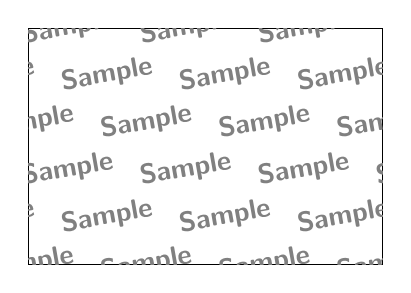
\begin{tikzpicture}
    \draw rectangle++(4.5,3);
    \clip rectangle++(4.5,3);
    \foreach\x in{0,1,2,3,4}{
      \foreach\y in{0,1,2,3,4,5,6}{
        \path(\x*1.5-\y*0.5,\y*0.6)node[rotate=10,text=gray]{\sffamily\bfseries\itshape Sample };
      }
    }
  \end{tikzpicture}
  %% 入れる画像：VS Code で ~/my_robot を開き、エクスプローラーにファイル一覧、エディタに README.md、下部に統合ターミナルを表示した状態のスクリーンショット（各部分に番号を付ける）
  % eps 画像を貼る場合は includegraphics をお使いください。
  % 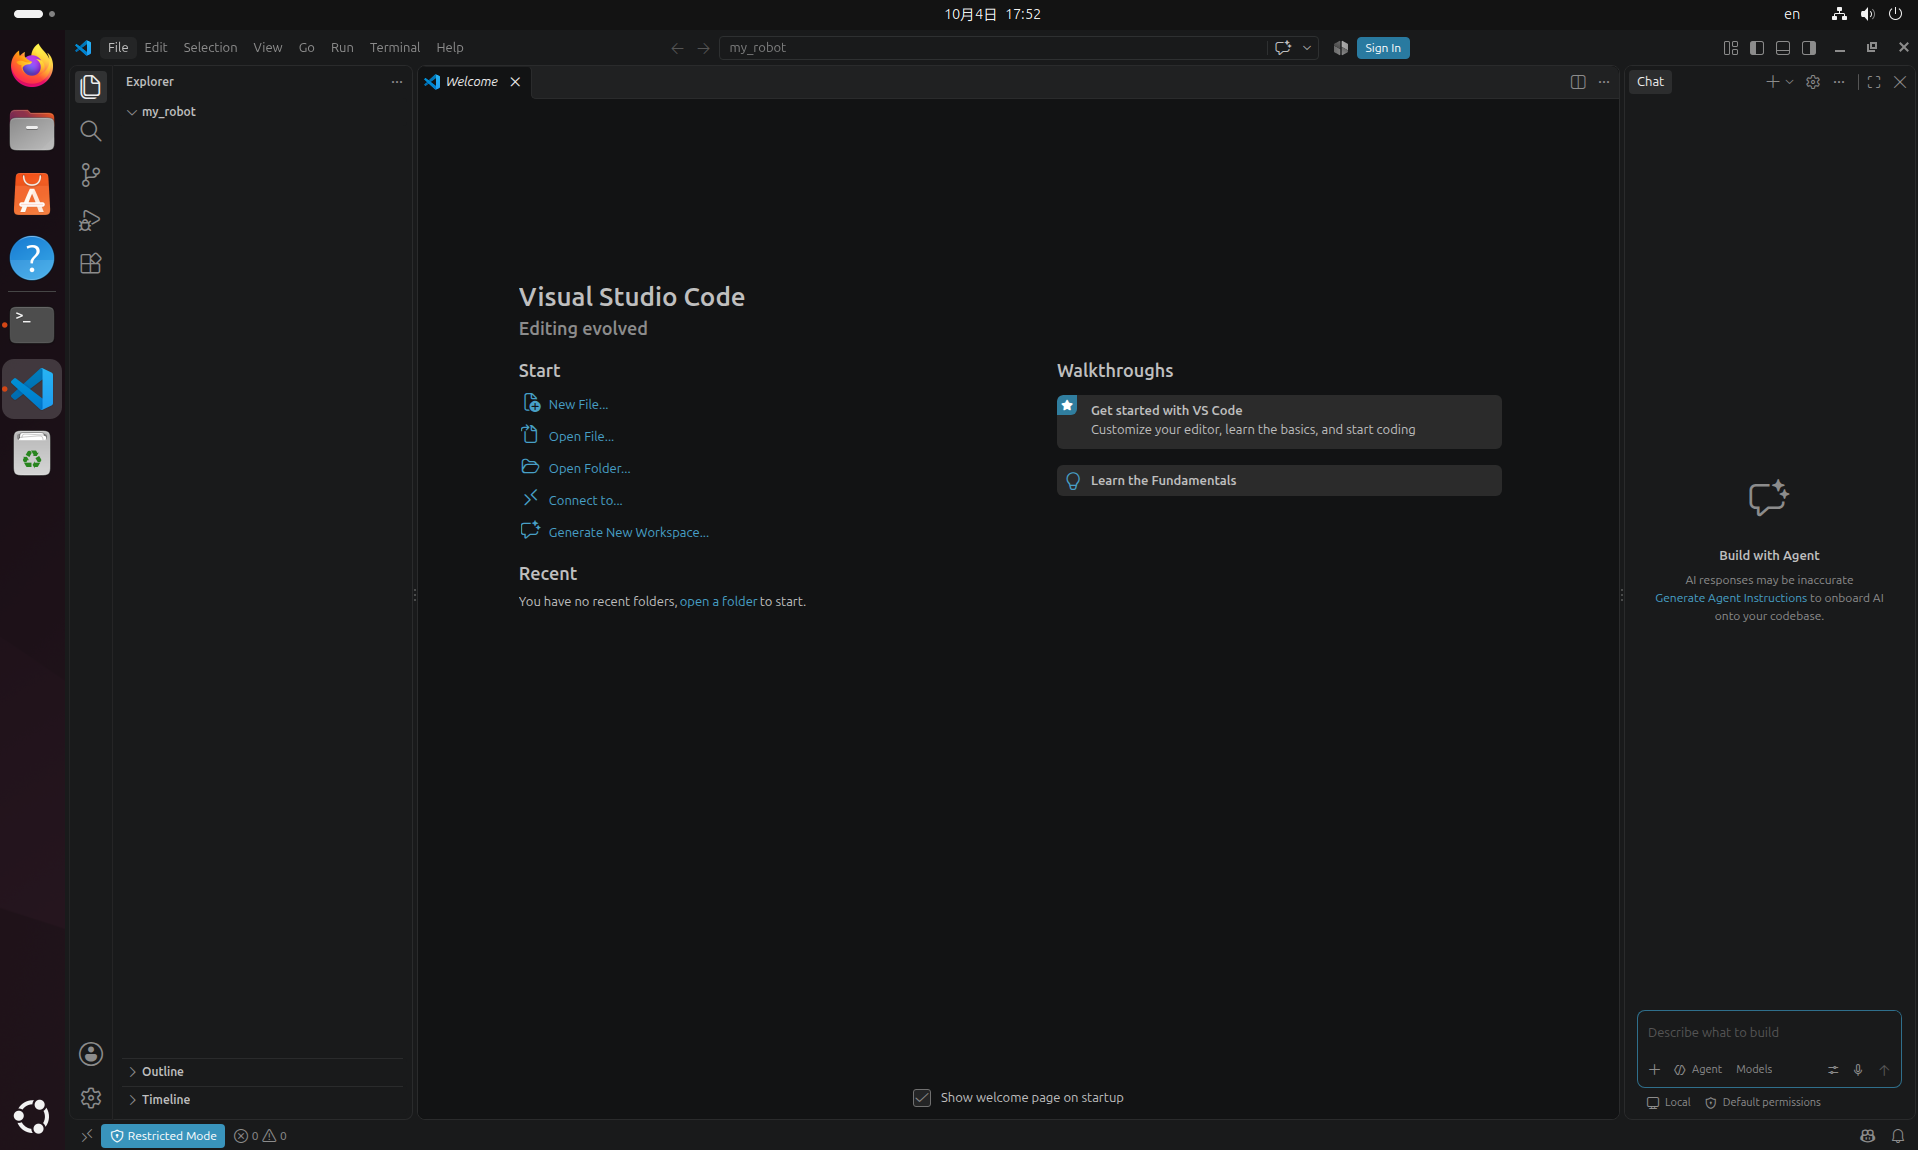
\includegraphics[width=0.8\linewidth]{editor/vscode_window.png}
  \caption{VS Code の画面}
  \label{fig:editor-vscode}
\end{figure}

\begin{description}
  \item[エクスプローラー] 左側に、開いているディレクトリの中のファイルが木構造で表示されます。クリックするとファイルが開きます。
  \item[エディタ] 中央で、ファイルを編集します。タブで複数のファイルを切り替えられます。
  \item[統合ターミナル] \key{Ctrl}+\key{`}（バッククォート）で、画面の下部にターミナルを開けます。エディタで編集しながら、同じ画面でコマンドを実行できます。
  \item[ソース管理] 左端のアイコンから、Git の変更の確認やコミットができます（\ref{chap:git}章）。
\end{description}

よく使うキー操作は、次のとおりです。

\begin{center}
  \begin{tabular}{ll}
    \toprule
    キー & 動作 \\
    \midrule
    \key{Ctrl}+\key{S} & 保存する \\
    \key{Ctrl}+\key{P} & ファイル名で探して開く \\
    \key{Ctrl}+\key{Shift}+\key{P} & コマンドパレット（すべての機能を名前で探して実行） \\
    \key{Ctrl}+\key{F} / \key{Ctrl}+\key{Shift}+\key{F} & ファイル内を検索 / すべてのファイルから検索 \\
    \key{Ctrl}+\key{`} & 統合ターミナルを開く・閉じる \\
    \key{Ctrl}+\key{/} & 選択した行をコメントにする・戻す \\
    \bottomrule
  \end{tabular}
\end{center}

\subsection{拡張機能}

左端の四角いアイコン（拡張機能）をクリックすると、拡張機能を検索してインストールできます。
ロボット開発では、まず次の拡張機能を入れておくとよいでしょう。

\begin{description}
  \item[Japanese Language Pack] メニューなどの表示を日本語にします。
  \item[Python] Python のプログラムの補完、エラーの表示、実行、デバッグができるようになります（第IV部）。
  \item[C/C++] C++ のプログラムの補完やエラーの表示ができるようになります。
  \item[YAML・XML] ROS 2 の設定ファイル（YAML）やパッケージの情報（XML）を編集しやすくします。
\end{description}

このほか、ROS 2 の開発を支援する拡張機能もあります。
拡張機能は便利ですが、入れすぎると動作が重くなるので、必要なものだけを入れるようにしましょう。

\subsection{リモート開発}
\label{sec:editor-remote}

VS Code には、別のコンピュータやコンテナの中のファイルを、手元の VS Code でそのまま編集できる機能があります。
これらの機能も、拡張機能として提供されています。

\begin{description}
  \item[Remote - SSH]
    SSH（\ref{sec:network-ssh}節）で接続したロボットの PC のファイルを、手元の PC の VS Code で編集できます。
    ファイルを開いたり保存したりする操作は、すべてロボットの PC の上のファイルに対して行われ、統合ターミナルもロボットの PC のシェルになります。
    ロボットの PC にモニタをつながなくても、手元と同じ快適さでプログラムを書き、その場で実行できるので、実機での開発では特に便利です。
    使い方は、拡張機能をインストールした後、コマンドパレット（\key{Ctrl}+\key{Shift}+\key{P}）で「Remote-SSH: Connect to Host」を選び、\cmd{user@192.168.1.20} や、\cmd{\textasciitilde/.ssh/config} で設定した名前（\cmd{robot}）を入力するだけです。
  \item[Dev Containers]
    Docker のコンテナ（\ref{chap:docker}章）の中に入って、VS Code で開発できます。
    ROS 2 の開発環境をコンテナとして用意しておけば、チーム全員が同じ環境で開発でき、自分の PC の環境を汚さずに済みます。
    詳しくは、\ref{chap:docker}章で説明します。
\end{description}

\begin{column}{エディタ戦争}
  「どのエディタが一番優れているか」は、昔からエンジニアの間で盛り上がる話題です。
  特に、1980 年代から続く vi（Vim）派と Emacs 派の論争は\textbf{エディタ戦争}と呼ばれ、半ば冗談として今も語り継がれています。

  vi 派は「モードを使いこなせば、指をほとんど動かさずに高速に編集できる」「どのコンピュータにも入っている」と主張し、Emacs 派は「何でもできる、自分だけの環境に育てられる」と譲りません。
  Emacs 派からは「vi の名前を 3 回続けると vi vi vi、ローマ数字で 6 6 6、つまり悪魔の数字だ」というジョークが、vi 派からは「Emacs はすばらしい OS だ。ただしエディタが付いていないのが残念だ」というジョークが飛んできます。
  Emacs の作者の Stallman が、「Emacs 教会」の聖人に扮して講演をしたこともあります。

  最近では、開発者を対象にした調査で VS Code が最も多く使われているという結果が続いていて、戦争の構図も変わってきました。
  とはいえ、VS Code にも Vim や Emacs のキー操作で使えるようにする拡張機能があり、長年の流儀は形を変えて生き続けています。

  結局のところ、一番よいエディタは「自分が快適に使えるエディタ」です。
  いろいろ試して、自分の手になじむ道具を見つけてください。
  ただし、どのエディタ派になるとしても、SSH でログインした先で困らないように、Vim の \cmd{:q!} だけは覚えておきましょう。
\end{column}

\section*{この章のまとめ}

\begin{itemize}
  \item プログラムや設定ファイルはテキストファイルで、エディタを使って編集します。
  \item nano は操作が簡単なターミナルエディタです。\key{Ctrl}+\key{O} で保存、\key{Ctrl}+\key{X} で終了します。
  \item Vim はモードを切り替えて使うエディタです。\key{i} で入力を始め、\key{Esc} で戻り、\cmd{:wq} で保存して終了、\cmd{:q!} で保存せずに終了します。
  \item Emacs は機能を自由に拡張できるエディタで、シェルのキー操作も Emacs と共通です。
  \item VS Code は拡張機能で機能を追加できる GUI エディタで、ふだんの開発の中心になります。Remote - SSH や Dev Containers を使うと、ロボットの PC やコンテナの中のファイルも手元で編集できます。
\end{itemize}

\chapter{Git によるバージョン管理}
\label{chap:git}

% この章で学ぶこと
\begin{goalbox}
  \begin{itemize}
    \item バージョン管理の考え方と、Git の基本的なしくみ
    \item \cmd{git add}, \cmd{git commit} などを使った変更の記録と確認
    \item ブランチを使った並行作業と、マージ
    \item GitHub を使った共有と、Pull Request による共同開発
    \item チームで開発するときの進め方
  \end{itemize}
\end{goalbox}

ロボットのプログラムは、一度書いたら終わりではありません。
パラメータを調整したり、新しい機能を試したり、不具合を直したりと、何度も書き換えながら育てていくものです。
この章では、その変更の歴史を記録し、チームで共有するための道具である \textbf{Git} の使い方を学びます。
Git は、ROS 2 を含む世界中のソフトウェア開発で使われている、エンジニアにとって必須の道具です。

\section{バージョン管理とは}
\label{sec:git-vcs}

\subsection{バージョン管理の必要性}

レポートを書くときに、\cmd{report.docx}, \cmd{report\_v2.docx}, \cmd{report\_final.docx}, \cmd{report\_final\_修正版.docx} のように、ファイルをコピーして残していった経験はないでしょうか。
この方法では、どれが最新なのか、それぞれ何を変えたのかがすぐにわからなくなります。
複数人で同じファイルを編集すれば、誰かの変更を上書きしてしまうこともあります。

\textbf{バージョン管理システム}は、ファイルの変更の歴史を記録し、管理するためのソフトウェアです。
バージョン管理システムを使うと、次のことができるようになります。

\begin{itemize}
  \item いつ、誰が、どのファイルの、どこを、なぜ変更したのかを記録できる
  \item 過去の任意の時点の状態に戻せる
  \item 「昨日までは動いていたのに」というときに、何を変えたのかを調べられる
  \item 複数人で同じプログラムを、互いの変更を壊さずに開発できる
\end{itemize}

ロボット開発では、「パラメータを変えたら動かなくなったので、前の状態に戻したい」という場面が頻繁にあります。
バージョン管理をしていれば、安心していろいろな変更を試すことができます。

\subsection{Git}

\textbf{Git} は、現在最も広く使われているバージョン管理システムです。
Git は、Linux カーネル（\ref{sec:linux-history}節）の開発を管理するために、2005 年に Linus Torvalds によって作られました。
世界中の開発者が参加する巨大なプロジェクトを管理するために作られただけあって、高速で、多人数での開発に強いのが特徴です。
Git 自体も OSS として公開されています。

Git は、Ubuntu では次のコマンドでインストールできます（\ref{chap:package}章）。

\begin{terminal}[Git をインストールする]
$ sudo apt install git
$ git --version
git version 2.43.0
\end{terminal}

\subsection{Git の基本的なしくみ}

Git を使ううえで、まず押さえておきたい言葉があります（図\ref{fig:git-areas}）。

\begin{figure}[tb]
  \centering
  % 図：Git の 4 つの領域とコマンド（chapters/tools/git.tex）
\begin{tikzpicture}[area/.style={figbox, minimum width=19mm, minimum height=13mm, font=\footnotesize}]
  \node[area] (work) at (0,0) {作業\\ディレクトリ};
  \node[area, fill=green!6] (stage) at (2.9,0) {ステージング\\エリア};
  \node[area, fill=blue!6] (local) at (5.8,0) {ローカル\\リポジトリ};
  \node[area, fill=orange!10] (remote) at (8.7,0) {リモート\\リポジトリ\\（GitHub）};
  \draw[figarrow] (work.east) -- node[figlabel, above]{\texttt{add}} (stage.west);
  \draw[figarrow] (stage.east) -- node[figlabel, above]{\texttt{commit}} (local.west);
  \draw[figarrow] (local.east) -- node[figlabel, above]{\texttt{push}} (remote.west);
  \draw[figarrow] (remote.north) -- ++(0,0.5) -| node[figlabel, pos=0.25, above]{\texttt{clone}（最初に丸ごとコピー）} (work.north);
  \draw[figarrow] (remote.south) -- ++(0,-1.2) -| node[figlabel, pos=0.25, below]{\texttt{pull}（変更を取り込み、作業ディレクトリにも反映）} (work.south);
  % 自分のコンピュータの範囲
  \draw[black!40, thick] ([xshift=-1mm,yshift=-2mm]work.south west) -- ++(0,-1.5mm) -| ([xshift=1mm,yshift=-2mm]local.south east);
  \node[figlabel, text=black!60, fill=white, inner sep=1pt] at ([yshift=-3.5mm]stage.south) {自分のコンピュータの中};
\end{tikzpicture}

  \caption{Git の 4 つの領域とコマンドの関係}
  \label{fig:git-areas}
\end{figure}

\begin{description}
  \item[リポジトリ]
    ファイルの変更の歴史を保存しておく場所です。
    Git で管理しているディレクトリの中の \cmd{.git} という隠しディレクトリが、リポジトリの実体です。
  \item[作業ディレクトリ]
    ふだんファイルを編集している、ディレクトリそのものです。
  \item[コミット]
    ある時点のファイルの状態を、リポジトリに記録することです。記録された 1 つ 1 つの状態のこともコミットと呼びます。
    ゲームのセーブのようなもので、いつでもその時点に戻ることができます。
  \item[ステージングエリア]
    次のコミットに含める変更を選んで置いておく、準備の場所です。
    Git では、変更したファイルをまずステージングエリアに登録し（\cmd{git add}）、それからまとめてコミットします（\cmd{git commit}）。
  \item[リモートリポジトリ]
    GitHub などのサーバの上に置いたリポジトリです。
    自分のコンピュータの中のリポジトリ（\textbf{ローカルリポジトリ}）の内容を送ったり（\cmd{git push}）、ほかの人の変更を取り込んだり（\cmd{git pull}）して、チームで共有します（\ref{sec:git-github}節）。
\end{description}

\subsection{最初の設定}

Git を使い始める前に、コミットに記録する名前とメールアドレスを設定します。
これは最初に 1 回だけ行えば十分です。

\begin{terminal}[Git の初期設定をする]
$ git config --global user.name "Taro Robot"
$ git config --global user.email "taro@example.com"
$ git config --global init.defaultBranch main
\end{terminal}

3 行目は、新しく作るリポジトリの最初のブランチ（\ref{sec:git-branch}節）の名前を \cmd{main} にする設定です。
GitHub で公開するつもりなら、メールアドレスは公開されても困らないものにしておきましょう。

\section{基本操作}
\label{sec:git-basic}

\subsection{リポジトリを作る}

練習用のディレクトリを作り、\cmd{git init} で Git の管理を始めます。

\begin{terminal}[リポジトリを作る]
$ mkdir ~/my_robot
$ cd ~/my_robot
$ git init
Initialized empty Git repository in /home/user/my_robot/.git/
\end{terminal}

\cmd{.git} というディレクトリが作られ、このディレクトリが Git で管理されるようになりました。

\subsection{状態を確認する}

エディタで \cmd{README.md} というファイルを作り、次の内容を書いて保存しましょう。

\begin{lstlisting}[caption={README.md}, label={lst:git-readme}]
# My Robot

ロボットを動かすプログラムです。
\end{lstlisting}

\begin{column}{README.md はなぜ必要か}
  \cmd{README}（read me、「私を読んで」）は、そのディレクトリやソフトウェアについて、最初に読んでほしいことを書いておくファイルです。
  ほとんどのリポジトリには、一番上のディレクトリに \cmd{README.md} が置かれています。
  名前を大文字にするのは、ファイルの一覧の中で目立たせるための昔からの習慣です。

  プログラムのファイルだけが並んでいても、ほかの人には、それが何のためのもので、どうやって動かせばよいのかがわかりません。
  半年後の自分も、書いた本人とはいえ、細かいことはほとんど覚えていないものです。
  そこで README には、たとえば次のようなことを書いておきます。
  \begin{itemize}
    \item このソフトウェアは何をするものか
    \item 動かすのに必要な環境（Ubuntu 24.04、ROS 2 Jazzy など）と、インストールやビルドの手順
    \item 使い方（実行するコマンドの例）
    \item ライセンス（\ref{sec:linux-oss}節）や、問い合わせ先
  \end{itemize}
  GitHub では、リポジトリのページを開くと \cmd{README.md} の内容が自動で表示されるので、README はそのリポジトリの「表紙」の役割も果たします。
  他人のソフトウェアを使うときも、まず README を読むのが基本です（\ref{sec:package-build}節）。

  拡張子の \cmd{.md} は、\textbf{Markdown}（マークダウン）という書き方で書かれていることを表しています。
  Markdown では、行頭に \cmd{\#} を付けると見出し、\cmd{-} を付けると箇条書きになるなど、簡単な記号で読みやすい文書を書くことができ、GitHub の上ではきれいに整形されて表示されます。
\end{column}

\cmd{git status} で、リポジトリの状態を確認します。
\cmd{git status} は、Git を使っていて迷ったときにまず実行するコマンドです。

\begin{terminal}[リポジトリの状態を確認する]
$ git status
On branch main

No commits yet

Untracked files:
  (use "git add <file>..." to include in what will be committed)
        README.md

nothing added to commit but untracked files present (use "git add" to track)
\end{terminal}

\cmd{Untracked files} は、「Git がまだ管理していないファイル」という意味です。

\subsection{変更を記録する}

\cmd{git add} で、\cmd{README.md} をステージングエリアに登録します。

\begin{terminal}[ステージングエリアに登録する]
$ git add README.md
$ git status
On branch main

No commits yet

Changes to be committed:
  (use "git rm --cached <file>..." to unstage)
        new file:   README.md
\end{terminal}

\cmd{Changes to be committed}（コミットされる変更）に \cmd{README.md} が入りました。
続いて、\cmd{git commit} でコミットします。
\cmd{-m} の後ろには、何を変更したのかを説明する\textbf{コミットメッセージ}を書きます。

\begin{terminal}[コミットする]
$ git commit -m "Add README"
[main (root-commit) 1a2b3c4] Add README
 1 file changed, 3 insertions(+)
 create mode 100644 README.md
\end{terminal}

これで、最初のコミットができました。
\cmd{1a2b3c4} は、このコミットを識別するための ID（\textbf{コミットハッシュ}）の先頭部分です。

\subsection{変更の差分を確認する}

\cmd{README.md} に、次の 2 行を書き足して保存してみましょう。

\begin{lstlisting}[caption={README.md（書き足した後）}, label={lst:git-readme2}]
# My Robot

ロボットを動かすプログラムです。

## 使い方
\end{lstlisting}

\cmd{git diff} を使うと、最後のコミットから何が変わったのか（\textbf{差分}）を確認できます。

\begin{terminal}[変更の差分を確認する]
$ git diff
diff --git a/README.md b/README.md
index 3b18e51..a3c9d2f 100644
--- a/README.md
+++ b/README.md
@@ -1,3 +1,5 @@
 # My Robot

 ロボットを動かすプログラムです。
+
+## 使い方
\end{terminal}

行頭の \cmd{+} は追加された行、\cmd{-} は削除された行を表しています。
コミットする前に \cmd{git diff} で変更内容を見直す習慣をつけると、意図しない変更をコミットしてしまうのを防げます。

確認できたら、先ほどと同じように \cmd{git add} と \cmd{git commit} を行います。
\cmd{git add .} と書くと、カレントディレクトリの下にある、変更されたすべてのファイルをまとめて登録できます。

\begin{terminal}[変更をまとめてコミットする]
$ git add .
$ git commit -m "Add usage section to README"
\end{terminal}

\subsection{履歴を見る}

これまでのコミットの履歴は、\cmd{git log} で確認できます。
\cmd{--oneline} を付けると、1 つのコミットを 1 行で簡潔に表示します。

\begin{terminal}[コミットの履歴を見る]
$ git log --oneline
5d6e7f8 (HEAD -> main) Add usage section to README
1a2b3c4 Add README
\end{terminal}

新しいコミットが上に表示されます。
\cmd{HEAD} は、今の作業ディレクトリがどのコミットを元にしているかを表す目印です。

\subsection{変更を取り消す}

ファイルを編集したものの、やはり変更をなかったことにしたいときは、\cmd{git restore} で最後のコミットの状態に戻せます。
ステージングエリアに登録した変更を取り消したい（ステージングエリアから外したい）ときは、\cmd{--staged} を付けます。

\begin{terminal}[変更を取り消す]
$ git restore README.md             # 編集した内容を捨てる
$ git restore --staged README.md    # git add を取り消す
\end{terminal}

\begin{caution}[git restore で捨てた変更は戻らない]
  \cmd{git restore ファイル名} を実行すると、コミットしていない編集内容は失われ、元に戻せません。
  一方、一度コミットしたものは、後からいつでも取り出せます。
  区切りのよいところで、こまめにコミットしておきましょう。
\end{caution}

\subsection{管理しないファイルを指定する}

プログラムをビルドしたときにできるファイルや、ログファイル、Python の仮想環境（\ref{sec:python-venv}節）のように、Git で管理する必要のないファイルもあります。
これらは、リポジトリの一番上に \cmd{.gitignore} というファイルを作って、名前やパターンを書いておくと、Git に無視させることができます。

\begin{lstlisting}[caption={.gitignore の例}, label={lst:git-gitignore}]
# ROS 2 のビルドで作られるディレクトリ
build/
install/
log/

# Python
__pycache__/
.venv/

# ログやデータ
*.log
\end{lstlisting}

\cmd{\#} で始まる行はコメントです。
\cmd{*} などのワイルドカード（\ref{sec:files-wildcard}節）も使えます。

\begin{point}[よいコミットのコツ]
  \begin{itemize}
    \item 1 つのコミットには、1 つのまとまった変更だけを入れる（「LiDAR の設定を追加」「速度の上限を変更」など）
    \item コミットメッセージには、何を変えたのかが一目でわかる短い説明を書く
    \item 動く状態でコミットする
    \item パスワードや API キーなどの秘密の情報や、センサの記録データのような大きなファイルはコミットしない
  \end{itemize}
\end{point}

\subsection{基本操作のまとめ}

ここまでに紹介したコマンドを、表にまとめておきます。

\begin{center}
  \begin{tabular}{lp{0.55\linewidth}}
    \toprule
    コマンド & 動作 \\
    \midrule
    \cmd{git init} & リポジトリを作る \\
    \cmd{git status} & 状態を確認する \\
    \cmd{git add ファイル} & 変更をステージングエリアに登録する \\
    \cmd{git commit -m "説明"} & コミットする \\
    \cmd{git diff} & コミットしていない変更の差分を見る \\
    \cmd{git log --oneline} & コミットの履歴を見る \\
    \cmd{git restore ファイル} & 編集した内容を捨てる \\
    \bottomrule
  \end{tabular}
\end{center}

\begin{column}{エディタから Git を使う}
  VS Code（\ref{chap:editor}章）には Git の機能が組み込まれていて、変更されたファイルの一覧や差分を画面で見ながら、ボタン操作でコミットすることもできます。
  ただし、画面の操作の裏側で実行されているのは、この章で学ぶコマンドと同じです。
  まずはコマンドで Git のしくみを理解しておくと、エディタの画面の意味もよくわかるようになります。
\end{column}

\section{ブランチとマージ}
\label{sec:git-branch}

\subsection{ブランチとは}

新しい機能を試しているうちに、プログラムが動かなくなってしまうことがあります。
ほかの人と共有しているプログラムでそれが起きると、みんなが困ってしまいます。
そこで Git では、\textbf{ブランチ}（枝）を使って、元のプログラムに影響を与えずに、別の流れで作業を進めることができます（図\ref{fig:git-branch}）。

\begin{figure}[tb]
  \centering
  % 図：ブランチとマージ（chapters/tools/git.tex）
\begin{tikzpicture}[commit/.style={circle, draw, thick, minimum size=4.5mm, inner sep=0pt, font=\scriptsize}]
  % main
  \node[commit, fill=blue!15] (a) at (0,0) {A};
  \node[commit, fill=blue!15] (b) at (1.5,0) {B};
  \node[commit, fill=blue!15] (e) at (4.5,0) {E};
  \node[commit, fill=blue!30, very thick] (m) at (7.5,0) {M};
  \draw[thick, blue!60!black] (a) -- (b) -- (e) -- (m);
  \node[anchor=east, font=\small\ttfamily, text=blue!60!black] at (-0.4,0) {main};
  % feature
  \node[commit, fill=orange!20] (c) at (3.0,-1.2) {C};
  \node[commit, fill=orange!20] (d) at (6.0,-1.2) {D};
  \draw[thick, orange!70!black] (b) -- (c) -- (d) -- (m);
  \node[anchor=east, font=\small\ttfamily, text=orange!70!black] at (2.6,-1.2) {feature/lidar};
  % 説明
  \node[figlabel, above=1mm of b] {ブランチを作る};
  \node[figlabel, above=1mm of m] {マージ};
  \node[figlabel, below=1mm of d, text=black!60] {新しい機能を試す};
  \node[figlabel, above=1mm of e, text=black!60] {main でも作業が進む};
\end{tikzpicture}

  \caption{ブランチとマージ}
  \label{fig:git-branch}
\end{figure}

リポジトリを作ると、最初は \cmd{main} というブランチが 1 つだけあります。
\cmd{main} ブランチは、常に動く状態に保っておくのが一般的です。
新しい機能を作るときは、\cmd{main} から新しいブランチを作り、そこで作業します。
うまくいったら、そのブランチの変更を \cmd{main} に取り込みます。
これを\textbf{マージ}といいます。
うまくいかなかったら、そのブランチを捨ててしまえば、\cmd{main} には何の影響も残りません。

\subsection{ブランチを作って切り替える}

\cmd{git switch -c ブランチ名} で、新しいブランチを作って切り替えます。
\cmd{git branch} で、ブランチの一覧と、今いるブランチ（\cmd{*} が付いたもの）を確認できます。

\begin{terminal}[ブランチを作って切り替える]
$ git switch -c feature/lidar
Switched to a new branch 'feature/lidar'
$ git branch
* feature/lidar
  main
\end{terminal}

このブランチの上で、ファイルを作ったり編集したりしてコミットしてみましょう。

\begin{terminal}[ブランチの上でコミットする]
$ echo "lidar_port: /dev/ttyUSB0" > lidar.yaml
$ git add lidar.yaml
$ git commit -m "Add LiDAR config"
\end{terminal}

\cmd{git switch main} で \cmd{main} ブランチに戻ると、\cmd{lidar.yaml} は作業ディレクトリから消えます。
\cmd{main} ブランチには、まだこのコミットが含まれていないからです。

\begin{terminal}[main ブランチに戻る]
$ git switch main
$ ls
README.md
\end{terminal}

\subsection{マージする}

\cmd{feature/lidar} ブランチの変更を \cmd{main} に取り込むには、\cmd{main} ブランチにいる状態で \cmd{git merge} を実行します。

\begin{terminal}[ブランチをマージする]
$ git merge feature/lidar
Updating 5d6e7f8..9a8b7c6
Fast-forward
 lidar.yaml | 1 +
 1 file changed, 1 insertion(+)
 create mode 100644 lidar.yaml
$ ls
README.md  lidar.yaml
\end{terminal}

マージが終わって不要になったブランチは、\cmd{git branch -d ブランチ名} で削除できます。

\subsection{コンフリクト}

2 つのブランチで同じファイルの同じ場所を別々に書き換えていると、Git はどちらの変更を採用すればよいか判断できません。
これを\textbf{コンフリクト}（衝突）といいます。
コンフリクトが起きると、Git はマージを途中で止めて、ファイルの中に両方の内容を書き込みます。

\begin{terminal}[コンフリクトが起きたときのファイルの中身]
<<<<<<< HEAD
max_speed: 0.5
=======
max_speed: 1.0
>>>>>>> feature/speed
\end{terminal}

\cmd{<<<<<<< HEAD} から \cmd{=======} までが今のブランチの内容、\cmd{=======} から \cmd{>>>>>>>} までがマージしようとしたブランチの内容です。
エディタでこのファイルを開き、正しい内容になるように書き直して、\cmd{<<<<<<<} などの印の行も消します。
その後、\cmd{git add} と \cmd{git commit} を行えば、マージが完了します。

\begin{terminal}[コンフリクトを解決してマージを完了する]
$ git add params.yaml
$ git commit -m "Merge feature/speed"
\end{terminal}

コンフリクトは失敗ではなく、Git が「人間が判断してください」と教えてくれている状態です。
落ち着いて、どちらの内容を残すべきかを考えましょう。

\section{GitHub との連携}
\label{sec:git-github}

\subsection{GitHub とは}

\textbf{GitHub} は、Git のリポジトリをインターネット上で保管・共有するための Web サービスです。
自分のリポジトリを置いてバックアップしたり、ほかのコンピュータと共有したり、チームで共同開発したりできます。
また、Linux カーネルや ROS 2 をはじめ、世界中の多くの OSS が GitHub で開発されています（\ref{sec:linux-oss}節）。
ROS 2 の本体も、\url{https://github.com/ros2} で公開されています。

GitHub を使うには、\url{https://github.com} でアカウントを作成します。

\begin{point}[Git と GitHub の違い]
  Git はバージョン管理のためのソフトウェアで、自分のコンピュータの中だけでも使えます。
  GitHub は、Git のリポジトリを置いておくためのインターネット上のサービスです。
  Git のリポジトリを置けるサービスには、GitHub のほかに GitLab などもあります。
\end{point}

\subsection{GitHub にログインする}

コマンドから GitHub を使うには、自分のアカウントであることを GitHub に証明する（認証する）必要があります。
最も手軽なのは、GitHub の公式のコマンドラインツール \cmd{gh} を使う方法です。

\begin{terminal}[gh を使って GitHub にログインする]
$ sudo apt install gh
$ gh auth login
? Where do you use GitHub? GitHub.com
? What is your preferred protocol for Git operations on this host? HTTPS
? Authenticate Git with your GitHub credentials? Yes
? How would you like to authenticate GitHub CLI? Login with a web browser
...
\end{terminal}

質問にはそれぞれ矢印キーで選んで \key{Enter} を押して答えます。
最後に表示されるコードを、自動で開く Web ブラウザの画面に入力すると、ログインが完了します。
SSH の鍵（\ref{sec:network-ssh}節）を GitHub に登録して認証する方法もよく使われます。

\subsection{リモートリポジトリに送る}

GitHub の Web ページで、新しいリポジトリ（ここでは \cmd{my\_robot}）を作成します。
作成したら、ローカルリポジトリにリモートリポジトリの場所を登録し、\cmd{git push} でコミットを送ります。

\begin{terminal}[GitHub のリポジトリにコミットを送る]
$ git remote add origin https://github.com/<ユーザ名>/my_robot.git
$ git push -u origin main
...
To https://github.com/<ユーザ名>/my_robot.git
 * [new branch]      main -> main
\end{terminal}

\cmd{origin} は、リモートリポジトリに付ける名前で、慣例として \cmd{origin} が使われます。
\cmd{-u} は、今後は \cmd{git push} だけで \cmd{origin} の \cmd{main} に送れるようにするオプションで、最初の 1 回だけ付けます。
GitHub のリポジトリのページを開くと、\cmd{README.md} などが表示されているはずです。

\subsection{リポジトリをコピーする・変更を取り込む}

GitHub にあるリポジトリを自分のコンピュータにコピーするには、\cmd{git clone} を使います。
ほかの人が公開しているロボットのプログラムを使うときや、別のコンピュータ（ロボットの PC など）で同じリポジトリを使うときに使います。

\begin{terminal}[リポジトリをコピーする]
$ git clone https://github.com/<ユーザ名>/my_robot.git
$ cd my_robot
\end{terminal}

リモートリポジトリに、ほかの人（または別のコンピュータの自分）が送った新しいコミットがあるときは、\cmd{git pull} で取り込みます。

\begin{terminal}[リモートリポジトリの変更を取り込む]
$ git pull
\end{terminal}

\subsection{Pull Request}

チームで開発するときや、ほかの人の OSS に貢献するときには、\textbf{Pull Request}（プルリクエスト、略して PR）という GitHub の機能を使います。
Pull Request は、「自分のブランチの変更を、\cmd{main} に取り込んでください」とお願いするための機能です。

\begin{enumerate}
  \item 作業用のブランチを作り、変更をコミットする
  \item \cmd{git push -u origin ブランチ名} で、ブランチを GitHub に送る
  \item GitHub の Web ページで、そのブランチから Pull Request を作成し、変更の内容や目的を説明する
  \item チームのメンバーが変更の内容を確認し（\textbf{レビュー}）、コメントを付ける
  \item 指摘があれば修正してコミットし、同じブランチに push する（Pull Request にも自動で反映される）
  \item 問題がなければ、GitHub の画面で \cmd{main} にマージする
\end{enumerate}

また、GitHub には、不具合の報告や改善の提案を書き込む \textbf{Issue} という機能もあります。
OSS を使っていて不具合を見つけたら、Issue で報告したり、修正を Pull Request で提案したりすることで、OSS の開発に貢献できます（\ref{sec:linux-oss}節）。

\section{チーム開発のワークフロー}
\label{sec:git-workflow}

\subsection{GitHub Flow}

複数人で開発するときは、ブランチや Pull Request をどのように使うかをあらかじめ決めておきます。
代表的な進め方が \textbf{GitHub Flow} と呼ばれるもので、次のようなシンプルなルールで運用します。

\begin{enumerate}
  \item \cmd{main} ブランチは、常に動く状態に保つ
  \item 作業を始めるときは、最新の \cmd{main} から、作業ごとにブランチを作る（\cmd{feature/lidar}, \cmd{fix/speed-limit} など）
  \item 作業用のブランチで、こまめにコミットし、GitHub に push する
  \item 作業が終わったら Pull Request を作り、ほかのメンバーにレビューしてもらう
  \item レビューで問題がなければ \cmd{main} にマージし、作業用のブランチは削除する
\end{enumerate}

\begin{terminal}[作業を始めるときの手順]
$ git switch main
$ git pull
$ git switch -c feature/lidar
\end{terminal}

作業を始める前に \cmd{git pull} で \cmd{main} を最新にしておくと、ほかの人の変更とのコンフリクトが起きにくくなります。

\subsection{チームで開発するときのルール}

\begin{itemize}
  \item 1 つの Pull Request は小さく保つ。大きな変更は、レビューが難しく、コンフリクトも起きやすくなる
  \item 同じファイルを複数人が同時に大きく書き換えないように、担当を決める（Issue で作業を宣言するのも有効）
  \item コミットメッセージや Pull Request の説明は、ほかの人が読んでわかるように書く
  \item \cmd{main} に直接コミットしない
\end{itemize}

実は本書の原稿も、GitHub のリポジトリで管理され、同じような流れで執筆されています。

\begin{caution}[\cmd{git push --force} は使わない]
  インターネット上の資料には、push がうまくいかないときに \cmd{git push --force} で強制的に送る方法が書かれていることがあります。
  このコマンドは、リモートリポジトリにあるほかの人のコミットを消してしまうおそれがあります。
  push が拒否されたときは、まず \cmd{git pull} でリモートの変更を取り込んでから、もう一度 push しましょう。
\end{caution}

\section*{この章のまとめ}

\begin{itemize}
  \item Git は、ファイルの変更の歴史を記録するバージョン管理システムです。変更は \cmd{git add} でステージングエリアに登録し、\cmd{git commit} でリポジトリに記録します。
  \item \cmd{git status} で状態を、\cmd{git diff} で差分を、\cmd{git log} で履歴を確認します。管理しないファイルは \cmd{.gitignore} に書きます。
  \item ブランチを使うと、\cmd{main} に影響を与えずに新しい作業を進められます。作業が終わったら \cmd{main} にマージします。
  \item GitHub は Git のリポジトリをインターネット上で共有するサービスです。\cmd{git push}, \cmd{git pull}, \cmd{git clone} でやり取りし、Pull Request でレビューを受けてからマージします。
  \item チームでは、\cmd{main} を常に動く状態に保ち、作業ごとにブランチを作って Pull Request で取り込む、という流れで開発します。
\end{itemize}

\chapter{ネットワークとリモート操作}
\label{chap:network}

% この章で学ぶこと
\begin{goalbox}
  \begin{itemize}
    \item IP アドレス・ホスト名・ポートといったネットワークの基礎
    \item \cmd{ip}, \cmd{ping}, \cmd{ss} によるネットワークの確認
    \item SSH による別のコンピュータへのログインと、鍵認証の設定
    \item \cmd{scp} と \cmd{rsync} によるファイルの転送
    \item tmux を使って、1 つのターミナルで複数の作業を同時に行う方法
  \end{itemize}
\end{goalbox}

ロボットに載っているコンピュータには、モニタやキーボードがつながっていないことがよくあります。
そのため、ロボットの開発では、手元の開発用 PC からネットワーク越しにロボットのコンピュータにログインして、プログラムを実行したり、ファイルを送ったりする作業が欠かせません。
また、ROS 2 のノードどうしの通信も、ネットワークを使って行われます。
この章では、ネットワークの基礎と、ロボット開発で毎日のように使うリモート操作の方法を学びます。

\section{IP アドレスとホスト名の基礎}
\label{sec:network-basics}

\subsection{IP アドレス}

ネットワークにつながったコンピュータには、それぞれを区別するための番号が割り当てられています。
これを \textbf{IP アドレス}といいます。
よく使われている IPv4 という形式では、\cmd{192.168.1.20} のように、0 から 255 までの 4 つの数字を \cmd{.} で区切って表します。
住所にたとえると、IP アドレスはネットワークの中での「番地」にあたります。

典型的なロボット開発の環境では、開発用 PC とロボットの PC が同じ Wi-Fi ルータにつながり、同じネットワークの中でそれぞれに IP アドレスが割り当てられます（図\ref{fig:network-robot}）。

\begin{figure}[tb]
  \centering
  % 図：開発用 PC とロボットのネットワーク構成（chapters/tools/network.tex）
\begin{tikzpicture}
  \node[figpart, minimum width=26mm, minimum height=14mm] (pc) at (0,0) {\textbf{開発用 PC}\\{\footnotesize\ttfamily 192.168.1.10}\\{\footnotesize\ttfamily dev-pc}};
  \node[figbox, minimum width=22mm, minimum height=10mm, fill=black!6] (router) at (4.0,0) {Wi-Fi ルータ\\{\footnotesize\ttfamily 192.168.1.1}};
  \node[figpart, minimum width=26mm, minimum height=14mm, fill=orange!10] (robot) at (8.0,0) {\textbf{ロボットの PC}\\{\footnotesize\ttfamily 192.168.1.20}\\{\footnotesize\ttfamily robot}};
  \draw[thick, dashed] (pc) -- node[figlabel, above]{Wi-Fi} (router);
  \draw[thick, dashed] (router) -- node[figlabel, above]{Wi-Fi} (robot);
  \draw[figarrow, {Stealth[length=2mm]}-{Stealth[length=2mm]}, blue!60!black] (pc.south) -- ++(0,-0.7) -| node[figlabel, pos=0.25, below, text=blue!60!black]{SSH でログイン・ファイル転送・ROS 2 の通信} (robot.south);
  \draw[thick, black!40] (router.north) -- ++(0,0.6) node[above, figlabel, text=black!60]{インターネット};
\end{tikzpicture}

  \caption{開発用 PC とロボットのネットワーク構成の例}
  \label{fig:network-robot}
\end{figure}

\begin{description}
  \item[プライベートアドレス]
    家庭や研究室の中のネットワーク（LAN）では、\cmd{192.168.x.x} や \cmd{10.x.x.x} といった、その中だけで使える IP アドレスが使われます。
    これを\textbf{プライベートアドレス}といいます。
  \item[localhost]
    \cmd{127.0.0.1} は、自分自身を表す特別な IP アドレスで、\textbf{localhost} とも呼ばれます。
  \item[DHCP]
    多くの場合、IP アドレスはルータが自動で割り当てます（\textbf{DHCP}）。
    そのため、再起動するとロボットの IP アドレスが変わってしまうことがあります。
    ロボットのように毎回同じ相手に接続したいコンピュータは、ルータの設定などで IP アドレスを固定しておくと便利です。
\end{description}

\subsection{ホスト名}

IP アドレスは数字の並びなので、覚えにくく、打ち間違えやすいものです。
そこで、コンピュータには\textbf{ホスト名}という名前も付けられています。
ホスト名は、プロンプトの \cmd{@} の後ろに表示されている名前です（\ref{sec:terminal-prompt}節）。

同じ LAN の中であれば、Ubuntu では \cmd{ホスト名.local} という名前で相手のコンピュータを指定できることが多くあります（mDNS というしくみを使っています）。
たとえば、ホスト名が \cmd{robot} のコンピュータには、\cmd{robot.local} という名前で接続できます。
ネットワークの環境によっては使えないこともあるので、そのときは IP アドレスを使いましょう。

\subsection{ポート}

1 台のコンピュータの中では、SSH や Web サーバなど、ネットワークを使う複数のプログラムが同時に動いています。
どのプログラムと通信するのかを区別するための番号を\textbf{ポート番号}といいます。
IP アドレスがマンションの住所だとすれば、ポート番号は部屋番号にあたります。
たとえば、SSH は 22 番、Web（HTTPS）は 443 番のポートを使うのが標準です。

\section{ネットワークの確認}
\label{sec:network-check}

\subsection{\cmd{ip}：IP アドレスを確認する}

自分のコンピュータの IP アドレスは、\cmd{ip address}（省略して \cmd{ip a}）で確認できます。

\begin{terminal}[IP アドレスを確認する]
$ ip a
1: lo: <LOOPBACK,UP,LOWER_UP> mtu 65536 qdisc noqueue state UNKNOWN group default qlen 1000
    inet 127.0.0.1/8 scope host lo
...
3: wlp2s0: <BROADCAST,MULTICAST,UP,LOWER_UP> mtu 1500 qdisc noqueue state UP group default qlen 1000
    link/ether 3c:22:fb:12:34:56 brd ff:ff:ff:ff:ff:ff
    inet 192.168.1.10/24 brd 192.168.1.255 scope global dynamic noprefixroute wlp2s0
...
\end{terminal}

たくさんの情報が表示されますが、まずは \cmd{inet} の行を見ます。
\cmd{lo} は自分自身を表す仮想的なネットワーク、\cmd{wlp2s0} は Wi-Fi のネットワークです（名前はコンピュータによって異なり、有線 LAN は \cmd{enp0s31f6} のような名前になります）。
この例では、Wi-Fi の IP アドレスが \cmd{192.168.1.10} であることがわかります。
末尾の \cmd{/24} は、先頭の 24 ビット（\cmd{192.168.1} の部分）が同じ IP アドレスどうしが同じネットワークに属する、という意味です。

IP アドレスだけを手早く知りたいときは、\cmd{hostname -I} も便利です。

\begin{terminal}[IP アドレスだけを表示する]
$ hostname -I
192.168.1.10
\end{terminal}

\subsection{\cmd{ping}：相手とつながっているか確認する}

\cmd{ping} は、相手のコンピュータに小さなデータを送り、返事が返ってくるかどうかで、通信できるかを確認するコマンドです。
\cmd{-c} オプションで、送る回数を指定できます。

\begin{terminal}[ロボットの PC と通信できるか確認する]
$ ping -c 3 192.168.1.20
PING 192.168.1.20 (192.168.1.20) 56(84) bytes of data.
64 bytes from 192.168.1.20: icmp_seq=1 ttl=64 time=3.21 ms
64 bytes from 192.168.1.20: icmp_seq=2 ttl=64 time=2.87 ms
64 bytes from 192.168.1.20: icmp_seq=3 ttl=64 time=4.02 ms

--- 192.168.1.20 ping statistics ---
3 packets transmitted, 3 received, 0% packet loss, time 2003ms
\end{terminal}

\cmd{time=} は、返事が返ってくるまでの時間（応答時間）です。
\cmd{0\% packet loss} であれば、すべての返事が返ってきています。
ロボットと通信できないときは、まず \cmd{ping} で相手に届いているかを確かめるのが、トラブル解決の第一歩です。
\cmd{-c} を付けずに実行した場合は、\key{Ctrl}+\key{C} で止めます。

\subsection{\cmd{ss}：通信を待ち受けているプログラムを確認する}

\cmd{ss} は、ネットワークの接続の状態を表示するコマンドです。
\cmd{-tln} オプションを付けると、どのポートで通信を待ち受けているかがわかります。

\begin{terminal}[待ち受けているポートを確認する]
$ ss -tln
State   Recv-Q  Send-Q   Local Address:Port    Peer Address:Port
LISTEN  0       4096           0.0.0.0:22           0.0.0.0:*
LISTEN  0       4096         127.0.0.1:631          0.0.0.0:*
...
\end{terminal}

この例では、22 番のポートで SSH のサーバが待ち受けていることがわかります。
次の節で SSH のサーバをインストールしたら、このコマンドで動いているかを確かめられます。

\section{SSH によるリモートログインと鍵認証}
\label{sec:network-ssh}

\subsection{SSH とは}

\textbf{SSH}（Secure Shell）は、ネットワーク越しに別のコンピュータにログインして、コマンドを実行するためのしくみです。
通信の内容はすべて暗号化されるので、パスワードや入力した内容を盗み見られる心配がありません。
SSH を使えば、手元の開発用 PC のターミナルから、ロボットの PC のシェルを操作できます。

SSH で接続するには、接続される側（ロボットの PC）で SSH の\textbf{サーバ}が動いている必要があります。
Ubuntu のデスクトップ版には SSH のサーバが入っていないので、ロボットの PC で次のようにインストールします。

\begin{terminal}[SSH のサーバを入れる（ロボット）]
$ sudo apt install openssh-server
\end{terminal}

インストールすると、SSH のサーバが自動的に起動し、22 番のポートで接続を待ち受けるようになります。

\subsection{ログインする}

開発用 PC から接続するには、\cmd{ssh ユーザ名@接続先} と入力します。
接続先には、IP アドレスかホスト名を指定します。

\begin{terminal}[ロボットの PC に SSH でログインする]
$ ssh user@192.168.1.20
The authenticity of host '192.168.1.20 (192.168.1.20)' can't be established.
ED25519 key fingerprint is SHA256:Xk3v...
Are you sure you want to continue connecting (yes/no/[fingerprint])? yes
user@192.168.1.20's password:
...
user@robot:~$
\end{terminal}

初めて接続する相手の場合は、「この相手を信頼してよいか」と聞かれるので、\cmd{yes} と入力します。
続いて、ロボットの PC のユーザのパスワードを入力すると、ログインできます。
プロンプトのホスト名が \cmd{robot} に変わったことに注目してください。
ここから先に入力するコマンドは、すべてロボットの PC の上で実行されます。

ログインを終了するには、\cmd{exit} と入力するか、\key{Ctrl}+\key{D} を押します。

\begin{caution}[今どのコンピュータを操作しているか]
  SSH でログインしていると、手元の PC とロボットの PC のターミナルが並んで、どちらで作業しているのかわからなくなりがちです。
  「ロボットの PC で実行するつもりのコマンドを、手元の PC で実行してしまった」といった事故を防ぐため、コマンドを入力する前にプロンプトのホスト名を確かめる習慣をつけましょう。
\end{caution}

\subsection{鍵認証}

毎回パスワードを入力するのは面倒ですし、推測されやすいパスワードを使うと、第三者に不正にログインされる危険もあります。
そこで SSH では、パスワードの代わりに\textbf{鍵}を使ってログインする\textbf{公開鍵認証}がよく使われます（図\ref{fig:network-ssh-key}）。

\begin{figure}[tb]
  \centering
  % 図：SSH の公開鍵認証（chapters/tools/network.tex）
\begin{tikzpicture}
  \node[figbox, minimum width=42mm, minimum height=28mm, fill=blue!4, anchor=north] (pc) at (0,0) {};
  \node[font=\small\bfseries, anchor=north] at (pc.north) {開発用 PC {\footnotesize\mdseries（接続する側）}};
  \node[figbox, minimum width=36mm, fill=red!8, font=\footnotesize, anchor=north] (priv) at (0,-0.75) {秘密鍵\\\texttt{\textasciitilde/.ssh/id\_ed25519}};
  \node[figbox, minimum width=36mm, fill=green!8, font=\footnotesize, anchor=north] (pub) at (0,-1.6) {公開鍵\\\texttt{\textasciitilde/.ssh/id\_ed25519.pub}};
  \node[figbox, minimum width=42mm, minimum height=28mm, fill=orange!6, anchor=north] (robot) at (6.2,0) {};
  \node[font=\small\bfseries, anchor=north] at (robot.north) {ロボットの PC {\footnotesize\mdseries（接続される側）}};
  \node[figbox, minimum width=36mm, fill=green!8, font=\footnotesize, anchor=north] (auth) at (6.2,-1.3) {登録された公開鍵\\\texttt{\textasciitilde/.ssh/authorized\_keys}};
  \draw[figarrow] (pub.east) -- node[figlabel, below, pos=0.5]{\tikz\node[fignum]{1}; \texttt{ssh-copy-id}} (auth.west |- pub.east);
  \draw[figarrow, {Stealth[length=2mm]}-{Stealth[length=2mm]}] (priv.east) -- node[figlabel, above, pos=0.5]{\tikz\node[fignum]{2}; 照合} (auth.west |- priv.east);
  \node[figlabel, text=red!60!black] at (0,-3.05) {秘密鍵は誰にも渡さない};
  \node[figlabel, text=black!60] at (6.2,-3.05) {公開鍵は渡しても安全};
\end{tikzpicture}

  \caption{SSH の公開鍵認証}
  \label{fig:network-ssh-key}
\end{figure}

公開鍵認証では、\textbf{秘密鍵}と\textbf{公開鍵}という、対になった 2 つの鍵を使います。
公開鍵を接続先に登録しておくと、SSH は、手元の秘密鍵が登録された公開鍵と対になっているかを確かめて、ログインを許可します。
公開鍵は南京錠、秘密鍵はその鍵にたとえられます。
南京錠（公開鍵）はいくつ配っても構いませんが、鍵（秘密鍵）は自分だけが持っていなければなりません。

まず、開発用 PC で \cmd{ssh-keygen} を実行して、鍵のペアを作ります。

\begin{terminal}[鍵のペアを作る（開発用 PC）]
$ ssh-keygen -t ed25519
Generating public/private ed25519 key pair.
Enter file in which to save the key (/home/user/.ssh/id_ed25519):
Enter passphrase (empty for no passphrase):
Enter same passphrase again:
Your identification has been saved in /home/user/.ssh/id_ed25519
Your public key has been saved in /home/user/.ssh/id_ed25519.pub
...
\end{terminal}

保存場所はそのまま \key{Enter} を押せば構いません。
\textbf{パスフレーズ}は、秘密鍵そのものを守るためのパスワードです。
設定しておくと、万が一秘密鍵のファイルが盗まれても、すぐには使われずに済みます。

次に、\cmd{ssh-copy-id} で公開鍵をロボットの PC に登録します。
このときだけ、ロボットの PC のパスワードを入力します。

\begin{terminal}[公開鍵を登録する（開発用 PC）]
$ ssh-copy-id user@192.168.1.20
...
Number of key(s) added: 1
\end{terminal}

これで、次からはパスワードを入力せずにログインできるようになります（パスフレーズを設定した場合は、パスフレーズを聞かれることがあります）。

\begin{caution}[秘密鍵は絶対に渡さない]
  \cmd{\textasciitilde/.ssh/id\_ed25519}（\cmd{.pub} の付いていないほう）が秘密鍵です。
  秘密鍵は、ほかの人に渡したり、GitHub などに公開したりしてはいけません。
  ほかのコンピュータやサービスに登録するのは、必ず \cmd{.pub} の付いた公開鍵のほうです。
\end{caution}

\subsection{接続の設定を保存する}

\cmd{\textasciitilde/.ssh/config} というファイルに接続先の情報を書いておくと、短い名前で接続できるようになります。

\begin{lstlisting}[caption={SSH の設定ファイル（\textasciitilde/.ssh/config）}, label={lst:network-ssh-config}]
Host robot
    HostName 192.168.1.20
    User user
\end{lstlisting}

\begin{terminal}[設定した名前で接続する]
$ ssh robot
user@robot:~$
\end{terminal}

\begin{column}{GUI のアプリをリモートで表示する}
  \cmd{ssh -X robot} のように \cmd{-X} オプションを付けて接続すると、ロボットの PC で起動した GUI のアプリの画面を、手元の PC に表示できます（X11 転送）。
  ただし、画面のデータをネットワークで送るため動作が重く、RViz のような 3D の表示には向いていません。
  ROS 2 では、GUI のツールは手元の PC で動かし、ネットワーク越しにロボットのノードと通信するのが一般的です（\ref{chap:ros2_install}章）。
\end{column}

\section{ファイル転送}
\label{sec:network-transfer}

\subsection{\cmd{scp}：ファイルをコピーする}

\cmd{scp} は、SSH を使ってコンピュータの間でファイルをコピーするコマンドです。
使い方は \cmd{cp}（\ref{sec:files-manipulate}節）と同じで、\cmd{scp コピー元 コピー先} と指定します。
別のコンピュータのファイルは、\cmd{接続先:パス} の形で表します。

\begin{terminal}[scp でファイルを転送する]
$ scp map.yaml robot:~/maps/             # 手元 → ロボット
$ scp robot:~/logs/run1.csv .            # ロボット → 手元
$ scp -r robot:~/logs ./robot_logs       # ディレクトリごと
\end{terminal}

接続先には、\cmd{\textasciitilde/.ssh/config} で設定した名前（\cmd{robot}）や、\cmd{user@192.168.1.20} を指定できます。
ディレクトリをコピーするときは、\cmd{cp} と同じく \cmd{-r} オプションを付けます。

\subsection{\cmd{rsync}：ディレクトリを同期する}

\cmd{rsync} は、ディレクトリの中身を同期（同じ状態に）するコマンドです。
2 回目以降は、変更のあったファイルだけを転送するので、大きなディレクトリでも短い時間で済みます。
手元の PC で編集したプログラムをロボットの PC に送る、といった作業に便利です。

\begin{terminal}[rsync でディレクトリを同期する]
$ rsync -av ~/ros2_ws/src/ robot:~/ros2_ws/src/
sending incremental file list
my_robot/my_robot/controller.py

sent 2,345 bytes  received 56 bytes  4,802.00 bytes/sec
total size is 48,210  speedup is 20.08
\end{terminal}

\cmd{-a} はファイルの権限や更新日時などをそのまま保ってコピーするオプション、\cmd{-v} は転送したファイルを表示するオプションです。
この例では、前回から変更された \cmd{controller.py} だけが転送されています。

\begin{caution}[rsync のパスの末尾の \cmd{/}]
  \cmd{rsync} では、コピー元のパスの末尾に \cmd{/} を付けるかどうかで意味が変わります。
  \cmd{src/} と書くと「\cmd{src} の中身」を、\cmd{src} と書くと「\cmd{src} ディレクトリそのもの」をコピーします。
  また、\cmd{--delete} オプションを付けると、コピー元にないファイルをコピー先から削除します。
  パスを間違えると大事なファイルを消してしまうので、慣れないうちは \cmd{-n}（実際には転送せず、何が起きるかだけを表示する）を付けて確かめてから実行しましょう。
\end{caution}

\section{tmux で複数ターミナルを管理する}
\label{sec:network-tmux}

\subsection{tmux とは}

SSH でロボットにログインして作業していると、次のような困りごとが出てきます。

\begin{itemize}
  \item ROS 2 では、複数のノードを同時に起動して、別のターミナルで様子を見ることが多い。そのたびに SSH で新しくログインするのは面倒
  \item Wi-Fi が一瞬切れただけで SSH の接続が切れ、ロボットの上で動かしていたプログラムも止まってしまう
\end{itemize}

これを解決するのが \textbf{tmux}（ティーマックス）です。
tmux を使うと、1 つのターミナルの画面を分割して、複数のシェルを同時に使えます（図\ref{fig:network-tmux}）。
さらに、tmux の中で動かしたプログラムは、SSH の接続が切れても動き続け、後から再び接続して続きの作業ができます。

\begin{figure}[tb]
  \centering
  % 図：tmux で画面を分割した様子（chapters/tools/network.tex）
\begin{tikzpicture}[pane/.style={draw, fill=black!3, anchor=north west, inner sep=2pt, align=left, font=\scriptsize\ttfamily}]
  \def\W{9.0} \def\H{4.2}
  \fill[ubuntutitlebar] (0,0) rectangle (\W,0.45);
  \node[font=\footnotesize\bfseries, text=white] at (\W/2,0.225) {user@robot: \textasciitilde};
  \draw[ubuntutitlebar, thick] (0,0.45) rectangle (\W,-\H);
  \draw[thick] (\W/2,0) -- (\W/2,-\H+0.35);
  \draw[thick] (\W/2,-1.9) -- (\W,-1.9);
  \node[pane, draw=none, fill=none] at (0.05,-0.05) {\$ ros2 launch my\_robot\\\ \ bringup.launch.py\\{[INFO]} [robot\_driver]: started\\{[INFO]} [lidar\_node]: started\\...};
  \node[pane, draw=none, fill=none] at (\W/2+0.05,-0.05) {\$ ros2 topic list\\/cmd\_vel\\/scan\\/odom};
  \node[pane, draw=none, fill=none] at (\W/2+0.05,-1.95) {\$ htop\\CPU [|||||      35\%]\\Mem [||||     1.2G]};
  \fill[green!50!black] (0,-\H+0.35) rectangle (\W,-\H);
  \node[font=\scriptsize\ttfamily, text=white, anchor=west] at (0.05,-\H+0.175) {[robot] 0:bash*};
  \node[figlabel, anchor=north, text=black!60] at (\W/2,-\H-0.1) {1 つのターミナルの中で、3 つのシェルを同時に使っている};
\end{tikzpicture}

  \caption{tmux で画面を分割した様子}
  \label{fig:network-tmux}
\end{figure}

tmux は、次のコマンドでインストールします。
SSH で使う場合は、ロボットの PC にインストールします。

\begin{terminal}[tmux をインストールする]
$ sudo apt install tmux
\end{terminal}

\subsection{セッションを作る}

tmux では、作業のまとまりを\textbf{セッション}と呼びます。
\cmd{tmux new -s セッション名} で、新しいセッションを作って開始します。

\begin{terminal}[tmux のセッションを開始する]
$ tmux new -s robot
\end{terminal}

画面の下に緑色の帯（ステータスバー）が表示されれば、tmux の中で作業している状態です。

\subsection{tmux の操作}

tmux の操作は、\textbf{プレフィックスキー}と呼ばれる \key{Ctrl}+\key{B} を押して離し、続けて操作ごとのキーを押して行います。
たとえば「\key{Ctrl}+\key{B} → \key{\%}」は、\key{Ctrl}+\key{B} を押して離してから \key{\%} を押す、という意味です。

\begin{center}
  \begin{tabular}{lp{0.5\linewidth}}
    \toprule
    キー操作 & 動作 \\
    \midrule
    \key{Ctrl}+\key{B} → \key{\%} & 画面を左右に分割する \\
    \key{Ctrl}+\key{B} → \key{"} & 画面を上下に分割する \\
    \key{Ctrl}+\key{B} → 矢印キー & 分割した画面（ペイン）を移動する \\
    \key{Ctrl}+\key{B} → \key{x} & 今のペインを閉じる \\
    \key{Ctrl}+\key{B} → \key{c} & 新しいウィンドウ（タブのようなもの）を作る \\
    \key{Ctrl}+\key{B} → \key{n} & 次のウィンドウに切り替える \\
    \key{Ctrl}+\key{B} → \key{d} & セッションから離れる（デタッチ） \\
    \bottomrule
  \end{tabular}
\end{center}

\subsection{セッションから離れる・戻る}

\key{Ctrl}+\key{B} → \key{d} を押すと、セッションを動かしたまま tmux の画面から離れることができます。
これを\textbf{デタッチ}といいます。
デタッチしても、セッションの中のプログラムは動き続けています。
SSH の接続が切れた場合も、自動的にデタッチした状態になります。

離れたセッションに戻る（\textbf{アタッチ}する）には、\cmd{tmux attach -t セッション名} を実行します。
動いているセッションの一覧は \cmd{tmux ls} で確認できます。

\begin{terminal}[セッションの一覧を確認して、戻る]
$ tmux ls
robot: 1 windows (created Wed Sep 30 10:15:32 2026)
$ tmux attach -t robot
\end{terminal}

セッションを完全に終了するには、セッションの中のすべてのシェルで \cmd{exit} を実行します。

\begin{point}[ロボットでの tmux の使い方]
  ロボットの PC に SSH でログインしたら、まず \cmd{tmux new -s robot}（2 回目以降は \cmd{tmux attach -t robot}）で tmux に入る習慣をつけましょう。
  ノードの起動、トピックの確認、CPU の使用率の監視などを、1 つの画面で並べて行えます。
  Wi-Fi が切れても、ロボットの上のプログラムは止まりません。
\end{point}

\begin{column}{ターミナルマルチプレクサのいろいろ}
  tmux のように、1 つのターミナルの中で複数のシェルを切り替えたり、画面を分割したりするソフトウェアを\textbf{ターミナルマルチプレクサ}といいます。
  ターミナルマルチプレクサは tmux だけではありません。
  古くから使われている GNU \textbf{screen} や、近年登場した、設定なしでも使いやすい \textbf{zellij} などもあります。

  最近では、生成 AI の発展によって、ターミナルマルチプレクサの新しい使い方が広がっています。
  Claude Code のような\textbf{コーディングエージェント}（ターミナルの中で動き、プログラムを書いたり実行したりする AI）を、ターミナルマルチプレクサの中に常駐させておき、複数のエージェントを並べて動かしたり、その様子を管理したりする使い方です。
  SSH の接続が切れても動き続けるというターミナルマルチプレクサの性質は、長い時間をかけて作業するエージェントとの相性がよいのです。
  そのため、コーディングエージェントを動かすことを前提にしたツールも登場してきています。

  \textbf{herdr}\footnote{\url{https://github.com/herdrdev/herdr}} は、「コーディングエージェントが住む場所」をうたうターミナルマルチプレクサです。
  tmux と同じように、接続が切れてもセッションが動き続けるうえに、それぞれのペインのエージェントが「作業中」「入力待ち」「待機中」のどの状態にあるかを一覧で確かめられます。
  SSH でつないだ別のコンピュータのエージェントもまとめて管理でき、Linux でも使えます。

  \textbf{cmux}\footnote{\url{https://github.com/manaflow-ai/cmux}} は、コーディングエージェントのためのターミナルアプリで、画面の分割やタブといったターミナルマルチプレクサの機能を持っています。
  エージェントが人間の確認を求めているときに通知で知らせてくれるのが特徴です。
  ただし、tmux のようにターミナルの中で動くものではなく、macOS 専用の GUI のアプリです。

  エージェントの助けを借りてロボットのプログラムを書く時代には、ターミナルマルチプレクサの使い方を知っていることが、ますます役に立つでしょう。
\end{column}

\section*{この章のまとめ}

\begin{itemize}
  \item ネットワーク上のコンピュータは IP アドレスで区別されます。ホスト名や \cmd{ホスト名.local} を使うと、名前で指定できます。通信するプログラムはポート番号で区別されます。
  \item \cmd{ip a} で IP アドレスを、\cmd{ping} で相手と通信できるかを、\cmd{ss} で待ち受けているポートを確認します。
  \item SSH を使うと、ネットワーク越しに別のコンピュータにログインできます。公開鍵認証を設定すると、パスワードなしで安全にログインできます。秘密鍵は誰にも渡してはいけません。
  \item \cmd{scp} でファイルをコピーし、\cmd{rsync} でディレクトリを同期します。
  \item tmux を使うと、1 つのターミナルで複数のシェルを使え、SSH の接続が切れてもプログラムが動き続けます。
\end{itemize}

\chapter{Docker 入門}
\label{chap:docker}

% この章で学ぶこと
\begin{goalbox}
  \begin{itemize}
    \item コンテナとは何か、仮想マシンとの違い
    \item Docker のインストールと、イメージ・コンテナの基本操作
    \item Dockerfile を書いて、自分用のイメージを作る方法
    \item コンテナの中で GUI アプリやデバイスを使う方法
    \item Docker Compose と Dev Containers を使った、ROS 2 の開発環境の構築
  \end{itemize}
\end{goalbox}

「自分の PC では動いたのに、ロボットの PC では動かない」「先輩の環境では動くのに、自分の環境では動かない」。
ソフトウェア開発では、このような環境の違いによるトラブルがよく起こります。
この章では、ソフトウェアとその動作環境をまるごとまとめて持ち運べるようにする \textbf{Docker} の使い方を学びます。

\section{コンテナとは}
\label{sec:docker-container}

\subsection{環境の違いという問題}

プログラムが動くかどうかは、プログラムそのものだけでなく、OS のバージョンや、インストールされているライブラリの種類とバージョンなど、そのコンピュータの\textbf{環境}に大きく左右されます。
ROS 2 のように多くのソフトウェアを組み合わせて使う場合は、特にその影響が大きくなります。
たとえば、ROS 2 Jazzy は Ubuntu 24.04 向けに作られているので、Ubuntu 22.04 の PC にはそのままインストールできません（\ref{sec:linux-distribution}節）。

\subsection{コンテナ}

\textbf{コンテナ}は、アプリケーションと、それが動くのに必要なライブラリや設定をひとまとめにして、ほかの部分から隔離された環境で動かすしくみです。
コンテナの中は、あたかも別のコンピュータのように見えます。
たとえば、Ubuntu 22.04 の PC の上で Ubuntu 24.04 のコンテナを動かし、その中で ROS 2 Jazzy を使う、といったことができます。
\textbf{Docker} は、このコンテナを作ったり動かしたりするための、最も広く使われているソフトウェアです。

コンテナを使うと、次のような利点があります。

\begin{itemize}
  \item 開発用 PC、ロボットの PC、チームのメンバーの PC で、まったく同じ環境を再現できる
  \item いろいろなソフトウェアを試しても、自分の PC の環境が汚れない（いらなくなったらコンテナを消すだけ）
  \item 異なるバージョンの ROS 2 を、1 台の PC で使い分けられる
\end{itemize}

\subsection{仮想マシンとの違い}

1 台の PC の上で別の OS を動かす方法には、VirtualBox などの\textbf{仮想マシン}もあります（\ref{sec:linux-setup}節）。
仮想マシンは、ハードウェアをまるごとソフトウェアで再現し、その上で OS（ゲスト OS）を丸ごと動かします。
一方、コンテナは、ホストの OS のカーネル（\ref{sec:linux-internals-kernel}節）をそのまま共有し、カーネルの機能を使ってプロセスを隔離しているだけです（図\ref{fig:docker-vm}）。

\begin{figure}[tb]
  \centering
  % 図：仮想マシンとコンテナの違い（chapters/tools/docker.tex）
\begin{tikzpicture}[layer/.style={draw, rounded corners=1.5pt, align=center, font=\footnotesize, minimum height=7mm, inner sep=1pt}]
  % 仮想マシン
  \node[font=\small\bfseries] at (2.1,4.35) {仮想マシン};
  \foreach \x/\a in {0/A,1.45/B,2.9/C} {
    \node[layer, fill=green!8, minimum width=13mm, anchor=south west, font=\scriptsize] at (\x,3.3) {アプリ \a};
    \node[layer, fill=orange!10, minimum width=13mm, anchor=south west, font=\scriptsize] at (\x,2.5) {ライブラリ};
    \node[layer, fill=blue!12, minimum width=13mm, anchor=south west, font=\scriptsize] at (\x,1.7) {ゲスト OS};
  }
  \node[layer, fill=black!8, minimum width=42mm, anchor=south west] at (0,0.9) {ハイパーバイザ};
  \node[layer, fill=blue!20, minimum width=42mm, anchor=south west] at (0,0.1) {ホスト OS};
  \node[layer, fill=black!15, minimum width=42mm, anchor=south west] at (0,-0.7) {ハードウェア};
  % コンテナ
  \node[font=\small\bfseries] at (7.6,4.35) {コンテナ};
  \foreach \x/\a in {5.5/A,6.95/B,8.4/C} {
    \node[layer, fill=green!8, minimum width=13mm, anchor=south west, font=\scriptsize] at (\x,2.5) {アプリ \a};
    \node[layer, fill=orange!10, minimum width=13mm, anchor=south west, font=\scriptsize] at (\x,1.7) {ライブラリ};
  }
  \node[layer, fill=black!8, minimum width=42mm, anchor=south west] at (5.5,0.9) {Docker};
  \node[layer, fill=blue!20, minimum width=42mm, anchor=south west] at (5.5,0.1) {ホスト OS（カーネルを共有）};
  \node[layer, fill=black!15, minimum width=42mm, anchor=south west] at (5.5,-0.7) {ハードウェア};
  \draw[black!30, dashed] (4.75,-0.8) -- (4.75,4.5);
\end{tikzpicture}

  \caption{仮想マシンとコンテナの違い}
  \label{fig:docker-vm}
\end{figure}

そのため、コンテナは仮想マシンに比べて、起動が速く（数秒以内）、メモリやストレージの使用量も少なくて済みます。
ただし、カーネルを共有しているので、Linux の上では Linux のコンテナしか直接は動かせません。

\subsection{イメージとコンテナ}

Docker を使ううえで、次の言葉を押さえておきましょう（図\ref{fig:docker-image}）。

\begin{figure}[tb]
  \centering
  % 図：イメージ・コンテナ・レジストリの関係（chapters/tools/docker.tex）
\begin{tikzpicture}
  \node[figpart, minimum width=24mm, minimum height=12mm, fill=orange!10] (hub) at (0,0) {\textbf{レジストリ}\\{\footnotesize（Docker Hub など）}};
  \node[figbox, minimum width=20mm, minimum height=12mm, fill=black!4] (file) at (0,-2.4) {\texttt{Dockerfile}\\{\footnotesize（設計図）}};
  \node[figpart, minimum width=22mm, minimum height=12mm] (img) at (3.9,-1.2) {\textbf{イメージ}\\{\footnotesize（ひな形）}};
  \node[figbox, minimum width=20mm, fill=green!8] (c1) at (7.9,-0.3) {コンテナ 1};
  \node[figbox, minimum width=20mm, fill=green!8] (c2) at (7.9,-1.2) {コンテナ 2};
  \node[figbox, minimum width=20mm, fill=green!8] (c3) at (7.9,-2.1) {コンテナ 3};
  \draw[figarrow] (hub.east) -- node[figlabel, above, sloped]{\texttt{docker pull}} (img.north west);
  \draw[figarrow] (file.east) -- node[figlabel, below, sloped]{\texttt{docker build}} (img.south west);
  \foreach \c in {c1,c2,c3} \draw[figarrow] (img.east) -- (\c.west);
  \node[figlabel, above] at (5.9,-0.75) {\texttt{docker run}};
\end{tikzpicture}

  \caption{イメージ・コンテナ・レジストリの関係}
  \label{fig:docker-image}
\end{figure}

\begin{description}
  \item[イメージ]
    コンテナのひな形です。
    OS の基本的なファイルや、インストール済みのソフトウェア、設定などがまとめて入っています。
    イメージそのものは読み取り専用で、変更されることはありません。
  \item[コンテナ]
    イメージから作られた、実際に動いている環境です。
    1 つのイメージから、いくつでもコンテナを作れます。
    料理にたとえると、イメージはレシピ、コンテナは実際に作った料理です。
  \item[レジストリ]
    イメージを保管・配布するための場所です。
    \textbf{Docker Hub}（\url{https://hub.docker.com}）には、Ubuntu や Python、ROS 2 など、さまざまな公式のイメージが公開されています。
  \item[Dockerfile]
    イメージの作り方を書いた設計図です（\ref{sec:docker-dockerfile}節）。
\end{description}

\section{イメージとコンテナの操作}
\label{sec:docker-basic}

\subsection{Docker のインストール}

Docker は、Docker 社の公式リポジトリを追加してインストールします（\ref{sec:package-repository}節）。
手順は変わることがあるので、実際には公式ドキュメント（\url{https://docs.docker.com/engine/install/ubuntu/}）を確認してください。
本書の執筆時点では、次のような手順です。

\begin{terminal}[Docker をインストールする]
$ sudo apt update
$ sudo apt install ca-certificates curl
$ sudo install -m 0755 -d /etc/apt/keyrings
$ sudo curl -fsSL https://download.docker.com/linux/ubuntu/gpg -o /etc/apt/keyrings/docker.asc
$ sudo chmod a+r /etc/apt/keyrings/docker.asc
$ echo "deb [arch=$(dpkg --print-architecture) signed-by=/etc/apt/keyrings/docker.asc] https://download.docker.com/linux/ubuntu $(. /etc/os-release && echo "$VERSION_CODENAME") stable" | sudo tee /etc/apt/sources.list.d/docker.list > /dev/null
$ sudo apt update
$ sudo apt install docker-ce docker-ce-cli containerd.io docker-buildx-plugin docker-compose-plugin
\end{terminal}

\ref{chap:package}章で学んだとおり、GPG 鍵を保存し、リポジトリを登録してから、\cmd{apt install} でインストールしています。

インストールが終わったら、自分のユーザを \cmd{docker} グループ（\ref{sec:linux-internals-users}節）に追加します。
こうすると、\cmd{docker} コマンドを \cmd{sudo} なしで実行できるようになります。
設定を反映させるために、一度ログアウトしてログインし直してください。

\begin{terminal}[docker グループに自分を追加する]
$ sudo usermod -aG docker $USER
\end{terminal}

\begin{caution}[docker グループの権限]
  \cmd{docker} グループのメンバーは、コンテナを通じて、実質的に root と同じ権限でシステムを操作できてしまいます。
  自分専用の開発用 PC では問題ありませんが、共用のコンピュータでは、誰を \cmd{docker} グループに入れるかに注意しましょう。
\end{caution}

動作を確認するために、\cmd{hello-world} というテスト用のイメージを動かしてみます。

\begin{terminal}[Docker の動作を確認する]
$ docker run hello-world
Unable to find image 'hello-world:latest' locally
latest: Pulling from library/hello-world
...
Hello from Docker!
This message shows that your installation appears to be working correctly.
...
\end{terminal}

手元に \cmd{hello-world} のイメージがなかったので、Docker Hub から自動でダウンロードしてから、コンテナを動かしたことがわかります。

\subsection{イメージを取得する}

Docker Hub からイメージをダウンロードするには、\cmd{docker pull} を使います。
イメージの名前の後ろの \cmd{:} に続く部分は\textbf{タグ}と呼ばれ、バージョンなどを表します。
ここでは、Ubuntu 24.04 のイメージを取得してみます。

\begin{terminal}[イメージを取得して一覧を見る]
$ docker pull ubuntu:24.04
$ docker images
REPOSITORY    TAG       IMAGE ID       CREATED       SIZE
ubuntu        24.04     b1d9df8ab815   3 weeks ago   78.1MB
hello-world   latest    d2c94e258dcb   1 year ago    13.3kB
\end{terminal}

\subsection{コンテナを動かす}

イメージからコンテナを作って動かすには、\cmd{docker run} を使います。
\cmd{-it} を付けると、コンテナの中のシェルを対話的に操作できます。

\begin{terminal}[コンテナの中のシェルを使う]
$ docker run -it --name test ubuntu:24.04 bash
root@3f2a1b4c5d6e:/# cat /etc/os-release | head -n 2
PRETTY_NAME="Ubuntu 24.04.1 LTS"
NAME="Ubuntu"
root@3f2a1b4c5d6e:/# exit
\end{terminal}

プロンプトが \cmd{root@3f2a1b4c5d6e:/\#} に変わりました。
これはコンテナの中のシェルで、ホスト名にはコンテナの ID が使われています。
コンテナの中では root ユーザとして動いていて、ホストの PC とは別の、まっさらな Ubuntu の環境になっています。
\cmd{exit} でシェルを終了すると、コンテナも停止します。

\cmd{docker run} のよく使うオプションは、次のとおりです。

\begin{center}
  \begin{tabular}{lp{0.6\linewidth}}
    \toprule
    オプション & 意味 \\
    \midrule
    \cmd{-it} & コンテナの中のシェルを対話的に操作する \\
    \cmd{--name 名前} & コンテナに名前を付ける \\
    \cmd{--rm} & コンテナが停止したら自動で削除する \\
    \cmd{-v ホストのパス:コンテナのパス} & ホストのディレクトリをコンテナの中から使えるようにする \\
    \cmd{-e 変数=値} & 環境変数（\ref{chap:env}章）を設定する \\
    \cmd{-d} & バックグラウンドで動かす \\
    \bottomrule
  \end{tabular}
\end{center}

\subsection{コンテナの管理}

コンテナの一覧は \cmd{docker ps} で確認できます。
\cmd{-a} を付けると、停止しているコンテナも表示されます。

\begin{terminal}[コンテナの一覧を見る]
$ docker ps -a
CONTAINER ID   IMAGE          COMMAND   CREATED         STATUS                     NAMES
3f2a1b4c5d6e   ubuntu:24.04   "bash"    2 minutes ago   Exited (0) 1 minute ago    test
\end{terminal}

停止したコンテナは、\cmd{docker start} で再び動かせます。
動いているコンテナの中で、別のシェルを開くには \cmd{docker exec} を使います。
ROS 2 では、1 つのコンテナの中で複数のノードを動かすために、この方法でシェルを追加することがよくあります。

\begin{terminal}[コンテナを再び動かして、シェルを開く]
$ docker start test
$ docker exec -it test bash
\end{terminal}

\begin{center}
  \begin{tabular}{lp{0.55\linewidth}}
    \toprule
    コマンド & 動作 \\
    \midrule
    \cmd{docker pull イメージ} & イメージを取得する \\
    \cmd{docker images} & イメージの一覧を見る \\
    \cmd{docker run イメージ} & コンテナを作って動かす \\
    \cmd{docker ps -a} & コンテナの一覧を見る \\
    \cmd{docker start 名前} / \cmd{stop 名前} & コンテナを動かす / 止める \\
    \cmd{docker exec -it 名前 bash} & 動いているコンテナでシェルを開く \\
    \cmd{docker rm 名前} & コンテナを削除する \\
    \cmd{docker rmi イメージ} & イメージを削除する \\
    \bottomrule
  \end{tabular}
\end{center}

\begin{caution}[コンテナの中の変更は消える]
  コンテナの中で作ったファイルやインストールしたソフトウェアは、そのコンテナを削除すると消えてしまいます。
  残しておきたいプログラムやデータは、\cmd{-v} オプションでホストのディレクトリを共有して、そこに保存しましょう。
  必要なソフトウェアは、次の節で説明する Dockerfile に書いておき、いつでも同じ環境を作り直せるようにするのが基本です。
\end{caution}

\section{Dockerfile の書き方}
\label{sec:docker-dockerfile}

\subsection{Dockerfile とは}

公式のイメージに、自分が必要なソフトウェアを追加したイメージを作りたいときは、\textbf{Dockerfile} を書きます。
Dockerfile には、元にするイメージと、そこに対して行う作業を順番に書きます。
Dockerfile があれば、誰でも、何度でも、同じイメージを作ることができます。

\subsection{Dockerfile の例}

ここでは、ROS 2 Jazzy の公式イメージに、亀のシミュレータ turtlesim を追加したイメージを作ってみます。
新しいディレクトリを作り、その中に \cmd{Dockerfile} という名前のファイルを作ります。

\begin{lstlisting}[style=bash, caption={Dockerfile}, label={lst:docker-dockerfile}]
# 元にするイメージ（ROS 2 Jazzy の公式イメージ）
FROM ros:jazzy

# 追加のパッケージをインストールする
RUN apt-get update && apt-get install -y \
    ros-jazzy-turtlesim \
    && rm -rf /var/lib/apt/lists/*

# 作業ディレクトリ
WORKDIR /root/ros2_ws

# コンテナを起動したときに実行するコマンド
CMD ["bash"]
\end{lstlisting}

主な命令の意味は、次のとおりです。

\begin{description}
  \item[FROM] 元にするイメージを指定します。Dockerfile の最初に書きます。
  \item[RUN] イメージを作るときに実行するコマンドを書きます。ここでは \cmd{apt-get} でパッケージをインストールしています。最後の \cmd{rm -rf /var/lib/apt/lists/*} は、不要になったパッケージの一覧を消して、イメージを小さくするためのものです。
  \item[WORKDIR] コンテナの中で作業するディレクトリを指定します。
  \item[COPY] ホストのファイルをイメージの中にコピーします（この例では使っていません）。
  \item[CMD] コンテナを起動したときに、標準で実行するコマンドを指定します。
\end{description}

\subsection{イメージを作って動かす}

Dockerfile からイメージを作るには、Dockerfile のあるディレクトリで \cmd{docker build} を実行します。
\cmd{-t} でイメージに名前（とタグ）を付けます。
最後の \cmd{.} は、カレントディレクトリの Dockerfile を使う、という意味です。

\begin{terminal}[イメージを作る]
$ docker build -t my_ros:jazzy .
...
 => => naming to docker.io/library/my_ros:jazzy
$ docker run -it --rm my_ros:jazzy
root@a1b2c3d4e5f6:~/ros2_ws# ros2 pkg list | grep turtlesim
turtlesim
\end{terminal}

turtlesim がインストールされたコンテナを動かせました。
ただし、turtlesim は GUI のウィンドウを開くアプリなので、このままでは画面を表示できません。
その方法を、次の節で説明します。

\section{GUI アプリやデバイスをコンテナで使う}
\label{sec:docker-gui-device}

\subsection{GUI アプリを表示する}

コンテナの中で起動した GUI アプリのウィンドウをホストの画面に表示するには、ホストの X サーバ（画面を描くしくみ）にコンテナからアクセスできるようにします。
まず、ホストで \cmd{xhost} コマンドを実行して、ローカルのコンテナからの接続を許可します。
次に、環境変数 \cmd{DISPLAY} と、X サーバとの通信に使うディレクトリをコンテナに渡して起動します。

\begin{terminal}[コンテナの中の GUI アプリを表示する]
$ xhost +local:
$ docker run -it --rm \
    -e DISPLAY=$DISPLAY \
    -v /tmp/.X11-unix:/tmp/.X11-unix \
    my_ros:jazzy \
    ros2 run turtlesim turtlesim_node
\end{terminal}

行末の \cmd{\textbackslash} は、長いコマンドを複数の行に分けて書くための記号です。
うまくいけば、ホストの画面に turtlesim のウィンドウが表示されます。
Ubuntu 24.04 の標準の画面（Wayland）でも、XWayland というしくみによって、この方法で表示できます。

\begin{caution}[xhost の設定]
  \cmd{xhost +local:} は、同じコンピュータの中のすべてのユーザやコンテナに、画面へのアクセスを許可する設定です。
  使い終わったら \cmd{xhost -local:} で元に戻しておくと安全です。
\end{caution}

RViz や Gazebo のように 3D の描画を行うアプリでは、GPU を使えるようにしないと動作が非常に遅くなります。
Intel や AMD の GPU では \cmd{--device /dev/dri} を、NVIDIA の GPU では NVIDIA Container Toolkit をインストールしたうえで \cmd{--gpus all} を、\cmd{docker run} に追加します。

\subsection{デバイスを使う}

USB でつないだセンサやマイコンをコンテナの中から使うには、\cmd{--device} オプションで、デバイスファイル（\ref{sec:linux-internals-device}節）をコンテナに渡します。

\begin{terminal}[USB のデバイスをコンテナに渡す]
$ docker run -it --rm --device /dev/ttyUSB0 my_ros:jazzy
\end{terminal}

すべてのデバイスにアクセスできるようにする \cmd{--privileged} というオプションもありますが、コンテナの隔離の意味がほとんどなくなってしまうので、できるだけ必要なデバイスだけを渡すようにしましょう。

\subsection{ネットワーク}

ROS 2 のノードは、ネットワークを通じてお互いを見つけ、通信します。
コンテナとホスト、あるいはコンテナと別の PC の ROS 2 のノードが通信できるようにするには、\cmd{--network host} を付けて、コンテナがホストと同じネットワークをそのまま使うようにするのが簡単です。
あわせて \cmd{--ipc host} も付けておくと、同じ PC の中のノード間の通信がうまくいかないトラブルを避けられます。

\begin{terminal}[ホストのネットワークを使うコンテナ]
$ docker run -it --rm --network host --ipc host my_ros:jazzy
\end{terminal}

\section{ROS 開発環境をコンテナで構築する}
\label{sec:docker-ros}

\subsection{ROS 2 の公式イメージ}

ROS 2 には、Docker Hub で公式のイメージが用意されています。
用途に合わせて、次のようなイメージを選びます。

\begin{center}
  \begin{tabular}{lp{0.55\linewidth}}
    \toprule
    イメージ & 内容 \\
    \midrule
    \cmd{ros:jazzy-ros-core} & ROS 2 の最小限の機能 \\
    \cmd{ros:jazzy}（\cmd{ros:jazzy-ros-base}） & 基本的な機能と、ビルドの道具 \\
    \cmd{osrf/ros:jazzy-desktop} & RViz などの GUI ツールやデモも含む \\
    \bottomrule
  \end{tabular}
\end{center}

試しに、2 つのターミナルでそれぞれコンテナを動かし、ROS 2 のデモのノードどうしを通信させてみましょう。
自分の PC に ROS 2 をインストールしていなくても、ROS 2 を体験できます。

\begin{terminal}[1 つ目のターミナル：メッセージを送るノード]
$ docker run -it --rm --network host --ipc host osrf/ros:jazzy-desktop \
    ros2 run demo_nodes_cpp talker
[INFO] [1727660000.123456789] [talker]: Publishing: 'Hello World: 1'
[INFO] [1727660001.123456789] [talker]: Publishing: 'Hello World: 2'
...
\end{terminal}

\begin{terminal}[2 つ目のターミナル：メッセージを受け取るノード]
$ docker run -it --rm --network host --ipc host osrf/ros:jazzy-desktop \
    ros2 run demo_nodes_cpp listener
[INFO] [1727660002.234567890] [listener]: I heard: [Hello World: 3]
...
\end{terminal}

2 つのコンテナの間で、メッセージがやり取りされていることがわかります。
ノードやメッセージの意味は、\ref{chap:ros2_concepts}章で学びます。
止めるときは、それぞれのターミナルで \key{Ctrl}+\key{C} を押します。

\subsection{Docker Compose で設定をまとめる}

ここまで見てきたように、ROS 2 のコンテナを動かす \cmd{docker run} のコマンドは、オプションが多くて長くなりがちです。
\textbf{Docker Compose} を使うと、これらの設定を \cmd{compose.yaml} というファイルに書いておき、短いコマンドでコンテナを起動できます。

\begin{lstlisting}[caption={compose.yaml}, label={lst:docker-compose}]
services:
  ros:
    build: .                     # 同じディレクトリの Dockerfile からイメージを作る
    image: my_ros:jazzy
    network_mode: host
    ipc: host
    environment:
      - DISPLAY=${DISPLAY}
    volumes:
      - /tmp/.X11-unix:/tmp/.X11-unix
      - ./ros2_ws/src:/root/ros2_ws/src   # 自分のプログラムを共有する
    devices:
      - /dev/ttyUSB0:/dev/ttyUSB0
    tty: true
\end{lstlisting}

\cmd{volumes} の 2 行目で、ホストの \cmd{./ros2\_ws/src} をコンテナの中の \cmd{/root/ros2\_ws/src} と共有しています。
ホストのエディタで書いたプログラムを、そのままコンテナの中でビルドして動かせます。

\begin{terminal}[Docker Compose でコンテナを起動する]
$ docker compose up -d           # バックグラウンドで起動する
$ docker compose exec ros bash   # コンテナの中のシェルを開く
$ docker compose down            # コンテナを停止して削除する
\end{terminal}

\subsection{VS Code の Dev Containers}

\ref{sec:editor-remote}節で紹介した VS Code の Dev Containers を使うと、VS Code そのものをコンテナの中に接続して開発できます。
プロジェクトのディレクトリに \cmd{.devcontainer/devcontainer.json} というファイルを置き、使う Dockerfile やオプションを書いておきます。

\begin{lstlisting}[caption={.devcontainer/devcontainer.json}, label={lst:docker-devcontainer}]
{
  "name": "ROS 2 Jazzy",
  "build": { "dockerfile": "../Dockerfile" },
  "runArgs": ["--network=host", "--ipc=host"],
  "customizations": {
    "vscode": {
      "extensions": ["ms-python.python"]
    }
  }
}
\end{lstlisting}

VS Code でこのディレクトリを開き、コマンドパレット（\key{Ctrl}+\key{Shift}+\key{P}）で「Dev Containers: Reopen in Container」を選ぶと、イメージが作られてコンテナが起動し、VS Code がコンテナの中に接続されます。
統合ターミナルもコンテナの中のシェルになり、指定した拡張機能もコンテナの中に自動でインストールされます。
\cmd{.devcontainer} ディレクトリを Git で共有しておけば（\ref{chap:git}章）、チームの誰もが同じ開発環境をすぐに用意できます。

\begin{point}[コンテナとの付き合い方]
  本書では、ROS 2 を Ubuntu 24.04 に直接インストールして使う方法を中心に説明します（\ref{chap:ros2_install}章）。
  そのほうが、しくみを理解しやすく、トラブルの原因も探しやすいからです。
  ROS 2 に慣れてきたら、チームでの開発や、異なるバージョンの ROS 2 を使い分けたいときに、コンテナを活用してみましょう。
\end{point}

\begin{column}{VirtualBox の中で Docker を使う}
  本書の環境では、VirtualBox の仮想マシンの中の Ubuntu に Docker をインストールしています（\ref{sec:linux-setup}節）。
  仮想マシンの中の Ubuntu はふつうの Ubuntu と同じなので、この章の手順はそのまま使えます。
  「仮想マシンの中でコンテナを動かす」と聞くと重そうに思えるかもしれませんが、コンテナは仮想マシンと違って OS を丸ごと動かすわけではないので、それほど負担にはなりません。

  なお、Windows や macOS には、Docker Desktop というアプリもあります。
  Docker Desktop も、内部で小さな Linux の仮想マシンを動かし、その上でコンテナを動かしています。
  ただし、GUI の表示や USB の機器の利用に追加の設定が必要なことが多く、大きな組織で使う場合には有料のライセンスも必要です。
  本書では、どの OS でも同じ手順で進められるよう、VirtualBox の中の Ubuntu で Docker を使います。
\end{column}

\section*{この章のまとめ}

\begin{itemize}
  \item コンテナは、アプリケーションとその動作環境をまとめて隔離して動かすしくみで、Docker はそのための代表的なソフトウェアです。仮想マシンと違ってホストのカーネルを共有するので、軽くて速く動きます。
  \item イメージはコンテナのひな形で、Docker Hub から \cmd{docker pull} で取得するか、Dockerfile から \cmd{docker build} で作ります。\cmd{docker run} でイメージからコンテナを作って動かします。
  \item コンテナを削除すると中の変更は消えるので、残したいファイルは \cmd{-v} でホストと共有し、必要なソフトウェアは Dockerfile に書いておきます。
  \item GUI アプリは \cmd{DISPLAY} と X サーバとの通信用のディレクトリを、デバイスは \cmd{--device} でコンテナに渡します。ROS 2 では \cmd{--network host} を使うと通信が簡単です。
  \item Docker Compose で設定をファイルにまとめたり、VS Code の Dev Containers でコンテナの中で直接開発したりできます。
\end{itemize}


\part{Python 入門}
\chapter{Python とは}
\label{chap:what_is_python}

% この章で学ぶこと
\begin{goalbox}
  \begin{itemize}
    \item Python がどのようなプログラミング言語なのか
    \item コンパイラ型言語とインタプリタ型言語の違い
    \item C 言語と比べたときの Python の特徴、メリットとデメリット
    \item ロボット開発での Python と C++ の使い分け
  \end{itemize}
\end{goalbox}

第IV部では、ROS 2 のプログラムを書くために必要な Python の基本を学びます。
この章ではまず、Python がどのような言語なのかを、C 言語と比べながら見ていきます。
プログラムとは何か、どんなプログラムも順次・分岐・繰り返しでできていること、については\ref{sec:computer-software}節で説明したので、忘れてしまった人は読み返してみてください。

\textbf{Python}（パイソン）は、1991 年に Guido van Rossum によって公開されたプログラミング言語です。
「読みやすく、書きやすい」ことを重視して設計されていて、プログラミングの入門から、Web サービス、データ分析、機械学習、そしてロボット開発まで、幅広い分野で使われています。
ROS 2 でも、C++ と並んで公式にサポートされている言語で、本書では Python を使って ROS 2 のプログラムを書きます（\ref{chap:rclpy}章）。

\section{コンパイラ型とインタプリタ型}
\label{sec:python-compile-interpret}

\ref{sec:computer-software}節で説明したように、CPU が直接理解できるのは機械語だけです。
人間がプログラミング言語で書いたプログラム（\textbf{ソースコード}）は、何らかの方法で機械語に翻訳してから実行する必要があります。
この翻訳の方法によって、プログラミング言語は大きく 2 つの種類に分けられます（図\ref{fig:python-compile-interpret}）。

\begin{figure}[tb]
  \centering
  % 図：コンパイラ型言語とインタプリタ型言語の実行の流れ（chapters/python/what_is_python.tex）
\begin{tikzpicture}
  % コンパイラ型（C 言語）
  \node[font=\small\bfseries, anchor=west] at (-1.1,1.25) {コンパイラ型（C 言語）};
  \node[figbox, minimum width=18mm] (csrc) at (0,0) {ソースコード\\{\footnotesize\ttfamily hello.c}};
  \node[figpart, minimum width=18mm] (cc) at (2.9,0) {コンパイラ\\{\footnotesize\ttfamily gcc}};
  \node[figbox, minimum width=18mm, fill=black!8] (bin) at (5.8,0) {実行ファイル\\{\footnotesize（機械語）}};
  \node[figbox, minimum width=14mm, fill=orange!10] (cpu1) at (8.5,0) {CPU};
  \draw[figarrow] (csrc) -- (cc);
  \draw[figarrow] (cc) -- node[figlabel, above]{翻訳} (bin);
  \draw[figarrow] (bin) -- node[figlabel, above]{実行} (cpu1);
  \node[figlabel, text=black!60] at (2.9,-0.95) {実行する前にまとめて翻訳};
  % インタプリタ型（Python）
  \node[font=\small\bfseries, anchor=west] at (-1.1,-1.85) {インタプリタ型（Python）};
  \node[figbox, minimum width=18mm] (psrc) at (0,-3.1) {ソースコード\\{\footnotesize\ttfamily hello.py}};
  \node[figpart, minimum width=47mm] (py) at (4.35,-3.1) {インタプリタ\\{\footnotesize\ttfamily python3}};
  \node[figbox, minimum width=14mm, fill=orange!10] (cpu2) at (8.5,-3.1) {CPU};
  \draw[figarrow] (psrc) -- (py);
  \draw[figarrow] (py) -- node[figlabel, above]{実行} (cpu2);
  \node[figlabel, text=black!60] at (4.35,-4.05) {1 行ずつ読みながら、その場で解釈して実行};
\end{tikzpicture}

  \caption{コンパイラ型言語とインタプリタ型言語の実行の流れ}
  \label{fig:python-compile-interpret}
\end{figure}

\begin{description}
  \item[コンパイラ型]
    実行する前に、\textbf{コンパイラ}というプログラムを使って、ソースコード全体をまとめて機械語の実行ファイルに翻訳しておく方式です。
    この翻訳の作業を\textbf{コンパイル}といいます。
    C 言語や C++ がこの方式の代表です。
    本にたとえると、外国語の本を、あらかじめ全部翻訳して翻訳書を作っておくようなものです。
  \item[インタプリタ型]
    \textbf{インタプリタ}というプログラムが、ソースコードを読みながら、その場で解釈して実行する方式です。
    事前に実行ファイルを作る必要はありません。
    Python はこの方式の代表です。
    本にたとえると、通訳の人に、外国語の本をその場で読み上げながら訳してもらうようなものです。
\end{description}

\section{C 言語と比べてみる}
\label{sec:python-vs-c}

同じ「画面に Hello, World! と表示する」プログラムを、C 言語と Python で書き比べてみましょう。

\begin{codelisting}[style=cpp]{C 言語のプログラム（hello.c）}{lst:python-hello-c}
#include <stdio.h>

int main(void)
{
    printf("Hello, World!\n");
    return 0;
}
\end{codelisting}

\begin{codelisting}[style=python]{Python のプログラム（hello.py）}{lst:python-hello-py}
print("Hello, World!")
\end{codelisting}

C 言語では、\cmd{main} という関数を用意し、その中に処理を書くという決まった形が必要です。
一方、Python では、やりたいことを 1 行書くだけで済みます。

実行の手順も異なります。
C 言語では、まず \cmd{gcc} というコンパイラで実行ファイルを作り、それから実行します。
Python では、\cmd{python3} というインタプリタにソースコードを渡すだけで、すぐに実行できます。

\begin{terminal}[C 言語のプログラムを実行する]
$ gcc hello.c -o hello
$ ./hello
Hello, World!
\end{terminal}

\begin{terminal}[Python のプログラムを実行する]
$ python3 hello.py
Hello, World!
\end{terminal}

プログラムを少し書き換えて試す、ということを何度も繰り返すときには、コンパイルの手間がない Python のほうが手軽です。

\section{Python の特徴}
\label{sec:python-features}

Python には、C 言語と比べて次のような特徴があります。

\begin{description}
  \item[書き方がシンプル]
    文の終わりに \cmd{;} を付けたり、処理のまとまりを \cmd{\{ \}} で囲んだりする必要がありません。
    代わりに、処理のまとまりを\textbf{インデント}（行頭の字下げ）で表します。
    インデントがそろっていないとエラーになるので、自然と読みやすいプログラムになります。
  \item[型を宣言しなくてよい]
    C 言語では、変数を使う前に「整数を入れる変数」「文字を入れる変数」のように\textbf{型}を宣言する必要があります（\textbf{静的型付け}）。
    Python では型の宣言は不要で、変数に入れた値によって型が自動的に決まります（\textbf{動的型付け}）。
  \item[メモリの管理が自動]
    C 言語では、必要なメモリを自分で確保し、使い終わったら自分で解放しなければなりません。
    解放を忘れたり、解放済みのメモリを使ったりすると、原因のわかりにくい不具合になります。
    Python では、使わなくなったメモリは自動的に解放されます（\textbf{ガベージコレクション}）。
  \item[ライブラリが豊富]
    数値計算の NumPy、画像処理の OpenCV、機械学習の PyTorch など、便利なライブラリ（プログラムの部品）が数多く公開されていて、簡単に利用できます（\ref{sec:python-pip}節）。
\end{description}

\section{メリットとデメリット}
\label{sec:python-pros-cons}

Python と C 言語（C++）には、それぞれ得意・不得意があります。

\begin{tablebox}[Python と C 言語・C++ の比較][tab:python-compare]
  \begin{tabular}{lp{0.33\linewidth}p{0.33\linewidth}}
    \toprule
     & Python & C 言語・C++ \\
    \midrule
    書きやすさ & 短く簡潔に書ける & 書く量が多く、決まりごとも多い \\
    試しやすさ & すぐに実行して試せる & 実行のたびにコンパイルが必要 \\
    実行速度 & 遅い & 速い \\
    メモリ管理 & 自動 & 自分で管理する（C++ には補助のしくみもある） \\
    エラーの発見 & 実行してみるまで見つからないことが多い & 型の誤りなどはコンパイル時に見つかる \\
    向いている用途 & 試作、処理の組み合わせ、データ処理、機械学習 & 速度が必要な処理、マイコン、ハードウェアに近い処理 \\
    \bottomrule
  \end{tabular}
\end{tablebox}

Python の最大のデメリットは、実行速度が遅いことです。
インタプリタがその場で解釈しながら実行するため、同じ処理でも、C 言語で書いたプログラムに比べて数十倍以上遅くなることがあります。
また、型の宣言がないため、型の間違いなどのミスが、実際にその行を実行するまで見つからないこともあります。

ただし、NumPy や OpenCV のような Python のライブラリの多くは、中身が C 言語や C++ で書かれています。
重い計算はライブラリの中の高速なプログラムに任せ、それらを組み合わせる部分を Python で書く、という使い方をすれば、書きやすさと速さを両立できます。

\begin{point}[ロボット開発での使い分け]
  ROS 2 では、Python で書くためのライブラリ（\cmd{rclpy}）と、C++ で書くためのライブラリ（\cmd{rclcpp}）が用意されています。
  Python で書いたノードと C++ で書いたノードは、同じように通信し合うことができます。
  そのため、まずは Python で手早く作って動かし、速度が必要になった部分だけを C++ で書き直す、という進め方がよく使われます。
  本書では、初めての人でも取り組みやすい Python を使います。
\end{point}

\section{Python のバージョン}
\label{sec:python-version}

Python には、大きく分けて Python 2 と Python 3 の 2 つの系統があります。
両者には互換性がなく、Python 2 で書かれたプログラムは、そのままでは Python 3 で動かないことがあります。
Python 2 は 2020 年にサポートが終了しているので、現在は Python 3 を使います。
Ubuntu 24.04 には、Python 3.12 が標準でインストールされています。

\begin{terminal}[Python のバージョンを確認する]
$ python3 --version
Python 3.12.3
\end{terminal}

インターネット上の古い情報には Python 2 向けのものも残っているので、参考にするときは注意しましょう。

\begin{column}{Python という名前}
  Python という名前は、ヘビのニシキヘビ（python）ではなく、作者の van Rossum が好きだったイギリスのコメディ番組「空飛ぶモンティ・パイソン」に由来しています。
  ただ、ロゴにはヘビの絵が使われています。
\end{column}

\section*{この章のまとめ}

\begin{itemize}
  \item Python は、読みやすく書きやすいことを重視したインタプリタ型のプログラミング言語です。
  \item C 言語のようなコンパイラ型の言語は実行前にまとめて機械語に翻訳し、Python のようなインタプリタ型の言語はその場で解釈しながら実行します。
  \item Python は書きやすく試しやすい反面、実行速度は C 言語や C++ に劣ります。重い処理は C 言語などで書かれたライブラリに任せるのが基本です。
  \item ROS 2 では Python（\cmd{rclpy}）と C++（\cmd{rclcpp}）の両方が使え、本書では Python を使います。
  \item 現在は Python 3 を使います。Ubuntu 24.04 には Python 3.12 が入っています。
\end{itemize}

\chapter{Python の開発環境}
\label{chap:python_env}

% この章で学ぶこと
\begin{goalbox}
  \begin{itemize}
    \item 対話モードとスクリプトファイルによる、Python のプログラムの実行方法
    \item pip を使った外部パッケージのインストール
    \item venv による仮想環境の作り方と使い方
    \item Ubuntu 24.04 で Python のパッケージを扱うときの注意点（PEP 668）と、ROS 2 との付き合い方
  \end{itemize}
\end{goalbox}

\ref{chap:what_is_python}章では、Python がどのような言語なのかを学びました。
この章では、Python のプログラムを実際に動かすための環境を整えます。

\section{プログラムの実行方法}
\label{sec:python-run}

Python のプログラムを実行する方法には、大きく分けて、対話モードで 1 行ずつ実行する方法と、スクリプトファイルに書いてまとめて実行する方法があります。

\subsection{\cmd{python3} コマンド}

Ubuntu 24.04 には Python 3 が最初からインストールされていて、\cmd{python3} というコマンドで実行できます。

\begin{terminal}[Python のバージョンを確認する]
$ python3 --version
Python 3.12.3
\end{terminal}

\begin{caution}[\cmd{python} ではなく \cmd{python3}]
  Ubuntu 24.04 では、\cmd{python} というコマンドは標準では用意されていません。
  インターネット上の資料に \cmd{python hello.py} と書かれていても、\cmd{python3 hello.py} と読み替えてください。
  どうしても \cmd{python} で実行したい場合は、\cmd{sudo apt install python-is-python3} で \cmd{python} を \cmd{python3} の別名として使えるようになります。
\end{caution}

\subsection{対話モード}

\cmd{python3} を引数なしで実行すると、\textbf{対話モード}（インタラクティブモード）が始まります。
\cmd{>>>} というプロンプトが表示され、Python の文を 1 行入力するたびに、その場で実行して結果を表示してくれます。

\begin{terminal}[対話モードで Python を使う]
$ python3
Python 3.12.3 (main, ...) [GCC 13.2.0] on linux
Type "help", "copyright", "credits" or "license" for more information.
>>> 1 + 2
3
>>> print("Hello, World!")
Hello, World!
>>> exit()
\end{terminal}

対話モードを終了するには、\cmd{exit()} と入力するか、\key{Ctrl}+\key{D} を押します。
対話モードは、ちょっとした計算をしたり、書き方を忘れた命令の動きを確かめたりするのに便利です。
第IV部の例の中で \cmd{>>>} から始まっているものは、対話モードで実行した例です。

\subsection{スクリプトファイル}

何行にもわたるプログラムは、テキストファイルに書いて保存し、まとめて実行します。
このファイルを\textbf{スクリプト}といい、拡張子は \cmd{.py} にするのが決まりです。
エディタ（\ref{chap:editor}章）で次の内容を書き、\cmd{hello.py} という名前で保存してみましょう。

\begin{codelisting}[style=python]{はじめてのスクリプト（hello.py）}{lst:python-env-hello}
name = "robot"
print("Hello, " + name + "!")
\end{codelisting}

保存したら、\cmd{python3} の引数にファイル名を指定して実行します。

\begin{terminal}[スクリプトを実行する]
$ python3 hello.py
Hello, robot!
\end{terminal}

\subsection{スクリプトを直接実行できるようにする}

スクリプトの 1 行目に次のような行を書いておくと、シェルスクリプト（\ref{chap:shellscript}章）と同じように、ファイルを直接実行できるようになります。
この行を \textbf{shebang}（シバン）といい、「このファイルは \cmd{python3} で実行する」ということをシェルに伝えます。

\begin{codelisting}[style=python]{shebang を付けたスクリプト（hello.py）}{lst:python-env-shebang}
#!/usr/bin/env python3
name = "robot"
print("Hello, " + name + "!")
\end{codelisting}

ファイルに実行権限を付ければ（\ref{chap:permission}章）、\cmd{./hello.py} で実行できます。

\begin{terminal}[スクリプトを直接実行する]
$ chmod +x hello.py
$ ./hello.py
Hello, robot!
\end{terminal}

ROS 2 のノードとして書く Python のファイルにも、この shebang を付けるのが一般的です。

\section{pip によるパッケージのインストール}
\label{sec:python-pip}

\subsection{パッケージと PyPI}

Python には、標準でさまざまな機能（\textbf{標準ライブラリ}）が付属していますが、それ以外にも、世界中の開発者が作った便利なプログラムの部品が数多く公開されています。
これらを\textbf{パッケージ}といい、多くは \textbf{PyPI}（Python Package Index、パイピーアイ）という Web サイトで公開されています。
数値計算の NumPy、画像処理の OpenCV（パッケージ名は \cmd{opencv-python}）、機械学習の PyTorch（パッケージ名は \cmd{torch}）なども、PyPI からインストールできます。

\subsection{pip の基本的な使い方}

PyPI のパッケージをインストールするには、\textbf{pip} というコマンドを使います。
Ubuntu 24.04 では pip は標準でインストールされていないので、次のようにインストールします。
あわせて、\ref{sec:python-venv}節で使う仮想環境の機能もインストールしておきましょう。

\begin{terminal}[pip と venv をインストールする]
$ sudo apt install python3-pip python3-venv
\end{terminal}

pip のよく使うコマンドは、次のとおりです。

\begin{tablebox}[pip のよく使うコマンド][tab:python-env-pip]
  \begin{tabular}{p{0.5\linewidth}p{0.42\linewidth}}
    \toprule
    コマンド & 動作 \\
    \midrule
    \cmd{pip install パッケージ名} & パッケージをインストールする \\
    \cmd{pip install パッケージ名==1.2.3} & バージョンを指定してインストールする \\
    \cmd{pip uninstall パッケージ名} & パッケージを削除する \\
    \cmd{pip list} & インストールされているパッケージの一覧を表示する \\
    \cmd{pip show パッケージ名} & パッケージの詳しい情報を表示する \\
    \bottomrule
  \end{tabular}
\end{tablebox}

ただし、Ubuntu 24.04 では、この表のコマンドをそのまま実行しても、パッケージをインストールできません。
その理由と、どうすればよいかを、次の\ref{sec:python-pep668}節で説明します。

\subsection{使っているパッケージを記録する}

プログラムがどのパッケージのどのバージョンを使っているかを記録しておくと、別のコンピュータでも同じ環境を再現できます。
\cmd{pip freeze} でインストールされているパッケージとバージョンの一覧を出力し、\cmd{requirements.txt} という名前のファイルに保存するのが慣例です（\cmd{>} については\ref{chap:text_pipe}章で説明しました）。
次は、数値計算の NumPy、グラフを描く Matplotlib、シリアル通信の pySerial などをインストールした環境での例です。
実際には、\ref{sec:python-venv}節の仮想環境の中で試します。

\begin{termexample}[パッケージを記録して再現する]
$ pip freeze > requirements.txt
$ cat requirements.txt
contourpy==1.3.0
matplotlib==3.9.2
numpy==2.1.1
pyserial==3.5
...
$ pip install -r requirements.txt
\end{termexample}

\cmd{requirements.txt} には、1 行に 1 つずつ、\cmd{パッケージ名==バージョン} の形でパッケージが並びます。
自分でインストールしたパッケージのほかに、それらが使っているパッケージ（\cmd{contourpy} は Matplotlib が使うパッケージです）も記録されます。
別のコンピュータでは、\cmd{pip install -r requirements.txt} で、書かれたパッケージをまとめて同じバージョンでインストールできます。

\section{Ubuntu 24.04 での注意点（PEP 668）}
\label{sec:python-pep668}

\subsection{\cmd{externally-managed-environment} エラー}

Ubuntu 24.04 で、\ref{sec:python-pip}節の \cmd{pip install} を試してみると、次のようなエラーが表示されます。

\begin{terminal}[仮想環境の外で pip install する]
$ pip install numpy
error: externally-managed-environment
...
\end{terminal}

これは、\textbf{PEP 668} という Python の取り決めに基づいた制限です\footnote{PEP（Python Enhancement Proposal）は、Python の機能や決まりごとを提案・記録するための文書で、番号で呼ばれます。}。
Ubuntu のシステムには、OS の一部として動いている Python のプログラムがたくさんあり、それらは \cmd{apt} で管理されたパッケージを使っています。
pip でシステムの Python のパッケージを書き換えてしまうと、\cmd{apt} で管理しているパッケージと食い違いが起きて、システムのツールが動かなくなるおそれがあります。
そこで、システムの Python は \cmd{apt} に管理を任せ、pip は仮想環境の中で使う、という役割分担が決められました。

\subsection{パッケージを入れる方法の選び方}

Ubuntu 24.04 で Python のパッケージを使いたいときは、次のように選びます。

\begin{enumerate}
  \item \textbf{apt で入れる}：
    よく使われるパッケージの多くは、\cmd{python3-} で始まる名前で Ubuntu のパッケージとしても提供されています（例：\cmd{sudo apt install python3-numpy}）。
    システム全体で使え、ROS 2 のノードからもそのまま使えます。
    ただし、バージョンは少し古いことがあります。
  \item \textbf{仮想環境の中で pip で入れる}：
    apt にないパッケージや、新しいバージョンが必要なパッケージは、\textbf{仮想環境}を作って、その中で pip で入れます。
  \item \textbf{pipx で入れる}：
    Python で書かれた「コマンドとして使うツール」をインストールしたいときは、\cmd{pipx} を使うと、ツールごとに自動で仮想環境を作ってインストールしてくれます（\cmd{sudo apt install pipx}）。
\end{enumerate}

\begin{caution}[\cmd{--break-system-packages} は使わない]
  エラーメッセージを検索すると、\cmd{pip install} に \cmd{--break-system-packages} というオプションを付けて制限を無視する方法が見つかります。
  名前のとおり「システムのパッケージを壊す」おそれがあるオプションなので、使わないようにしましょう。
  同じ理由で、\cmd{sudo pip install} も使ってはいけません。
\end{caution}

本書では、Python の練習で使うパッケージは 2 の仮想環境に、ROS 2 のノードで使うパッケージは 1 の apt で入れることにします。
次の節では、仮想環境の作り方と使い方を学びます。

\section{venv による仮想環境}
\label{sec:python-venv}

\subsection{仮想環境とは}

複数のプログラムを開発していると、「プログラム A では NumPy の新しい版を使いたいが、古いプログラム B は古い版でないと動かない」といった問題が起こります。
1 つの Python に 1 つのバージョンのパッケージしか入れられないと、この問題は解決できません。

そこで使うのが\textbf{仮想環境}です。
仮想環境は、Python のパッケージを入れるための独立した場所を、プロジェクトごとに作るしくみです（図\ref{fig:python-env-venv}）。
仮想環境の中で \cmd{pip install} したパッケージは、その仮想環境の中だけで使われ、システムやほかの仮想環境には影響しません。
Python には、仮想環境を作るための \textbf{venv} という機能が標準で用意されています。

\begin{figure}[tb]
  \centering
  % 図：システムの Python と仮想環境の関係（chapters/python/python_env.tex）
\begin{tikzpicture}
  % システムの Python
  \node[figpart, minimum width=96mm, minimum height=15mm, anchor=north west, fill=blue!10] (sys) at (0,0) {};
  \node[font=\small\bfseries, anchor=north west] at (sys.north west) {システムの Python（\texttt{/usr/bin/python3}）};
  \node[figlabel, anchor=south west, align=left] at ([xshift=1.5mm,yshift=1.5mm]sys.south west)
    {apt で入れたパッケージ（\texttt{python3-numpy} など）、ROS 2 の \texttt{rclpy} など\\
     {\color{red!60!black} \texttt{pip} で直接パッケージを入れることはできない（PEP 668）}};
  % 仮想環境
  % 仮想環境（3 つの例）
  \node[figbox, minimum width=29mm, minimum height=19mm, anchor=north west, fill=green!6] (v) at (0,-2.1) {};
  \node[font=\footnotesize\bfseries, anchor=north west] at (v.north west) {\texttt{robot\_ai}};
  \node[figlabel, anchor=north west, align=left] at ([xshift=1.5mm,yshift=-5mm]v.north west) {\ttfamily torch\\\ttfamily opencv-python};
  \node[figbox, minimum width=29mm, minimum height=19mm, anchor=north west, fill=green!6] (v) at (3.3,-2.1) {};
  \node[font=\footnotesize\bfseries, anchor=north west] at (v.north west) {\texttt{web\_tool}};
  \node[figlabel, anchor=north west, align=left] at ([xshift=1.5mm,yshift=-5mm]v.north west) {\ttfamily flask\\\ttfamily requests};
  \node[figbox, minimum width=29mm, minimum height=19mm, anchor=north west, fill=green!6] (v) at (6.6,-2.1) {};
  \node[font=\footnotesize\bfseries, anchor=north west] at (v.north west) {\texttt{old\_project}};
  \node[figlabel, anchor=north west, align=left] at ([xshift=1.5mm,yshift=-5mm]v.north west) {\ttfamily numpy\\\rmfamily （古い版）};
  \node[figlabel, text=black!60] at (4.8,-4.55) {仮想環境ごとに、別々のパッケージやバージョンを入れられる};
  \draw[figarrow, dashed, black!50] (4.8,-1.55) -- node[figlabel, right, text=black!60]{Python 本体を共有} (4.8,-2.05);
\end{tikzpicture}

  \caption{システムの Python と仮想環境の関係}
  \label{fig:python-env-venv}
\end{figure}

\subsection{仮想環境を作る}

仮想環境は、\cmd{python3 -m venv 仮想環境のディレクトリ名} で作ります。
プロジェクトのディレクトリの中に \cmd{.venv} という名前で作るのが一般的です。

\begin{terminal}[仮想環境を作る]
$ mkdir ~/py_practice
$ cd ~/py_practice
~/py_practice$ python3 -m venv .venv
~/py_practice$ ls -a
.  ..  .venv
\end{terminal}

\cmd{.venv} ディレクトリの中に、この仮想環境専用の \cmd{python3} や \cmd{pip}、パッケージを入れる場所が作られます。

\subsection{仮想環境を有効にする}

作った仮想環境を使うには、\cmd{source} コマンド（\ref{chap:env}章）で仮想環境を\textbf{有効化}（activate）します。
有効化すると、プロンプトの先頭に仮想環境の名前が表示されます。

\begin{terminal}[仮想環境を有効にする]
~/py_practice$ source .venv/bin/activate
(.venv) user@robot:~/py_practice$
\end{terminal}

この状態で \cmd{python3} や \cmd{pip} を実行すると、仮想環境の中のものが使われます。
\cmd{which} コマンド（\ref{sec:terminal-relation}節）で確かめてみましょう。

\begin{terminal}[仮想環境の python3 を確かめる]
~/py_practice$ which python3
/home/user/py_practice/.venv/bin/python3
\end{terminal}

仮想環境の中であれば、\cmd{pip install} でパッケージをインストールできます。

ここでは、数値計算の NumPy と、シリアル通信（マイコンなどとの通信）の pySerial をインストールしてみます。
パッケージ名を空白で区切って並べると、まとめてインストールできます。

\begin{terminal}[仮想環境でパッケージを入れる]
~/py_practice$ pip install numpy pyserial
Collecting numpy
...
Successfully installed numpy-2.1.1 pyserial-3.5
~/py_practice$ python3 -c "import numpy; print(numpy.__version__)"
2.1.1
\end{terminal}

\cmd{python3 -c} は、後ろに書いた Python の文を実行するオプションです。
ここでは、NumPy が読み込めることと、そのバージョンを確かめています（バージョンの数字は、インストールした時期によって変わります）。

\ref{sec:python-pip}節の \cmd{pip freeze} で、インストールしたパッケージを記録してみましょう。

\begin{terminal}[仮想環境のパッケージを記録する]
~/py_practice$ pip freeze > requirements.txt
~/py_practice$ cat requirements.txt
numpy==2.1.1
pyserial==3.5
\end{terminal}

仮想環境の中で実行すると、その仮想環境にインストールしたパッケージだけが記録されます。

\subsection{仮想環境を終了する}

仮想環境を終了するには、\cmd{deactivate} と入力します。
プロンプトの先頭の \cmd{(.venv)} が消え、システムの Python に戻ります。

\begin{terminal}[仮想環境を終了する]
~/py_practice$ deactivate
user@robot:~/py_practice$
\end{terminal}

仮想環境は、ターミナルを開くたびに有効化し直す必要があります。
いらなくなった仮想環境は、ディレクトリごと削除すれば消えます（\cmd{rm -r .venv}）。

\begin{point}[仮想環境の使い方のまとめ]
  \begin{itemize}
    \item 作る：\cmd{python3 -m venv .venv}（プロジェクトごとに 1 回）
    \item 有効にする：\cmd{source .venv/bin/activate}（ターミナルを開くたびに）
    \item パッケージを入れる：\cmd{pip install パッケージ名}
    \item 終了する：\cmd{deactivate}
  \end{itemize}
  \cmd{.venv} ディレクトリはコンピュータごとに作り直すものなので、Git で管理するときは含めないようにします（\ref{chap:git}章）。
  代わりに \cmd{requirements.txt} を管理しておきましょう。
\end{point}

\begin{column}{venv 以外の開発ツール：uv・pixi・Anaconda}
  仮想環境やパッケージを管理するツールは、venv と pip のほかにもあります。

  \textbf{uv}：
  近年、急速に利用者を増やしているツールです。
  Rust という高速な言語で作られていて、開発元によれば pip の 10〜100 倍の速さでパッケージをインストールできます。
  仮想環境の作成（\cmd{uv venv}）、パッケージのインストール（\cmd{uv pip install}）、Python 本体のバージョンの切り替えまで、1 つのコマンドでこなせます。

  \textbf{pixi}：
  conda 形式のパッケージを扱う、uv と同じく Rust 製の高速なツールです。
  C/C++ のライブラリなど Python 以外のソフトウェアもまとめて管理でき、RoboStack というプロジェクトと組み合わせると、apt を使わずに ROS 2 の環境を作ることもできます。

  \textbf{Anaconda}：
  データ分析や機械学習の分野で古くから使われている、よく使うライブラリをまとめた Python の配布パッケージです。
  容量が大きく、組織で使う場合は有料のライセンスが必要になることがあります。

  uv は venv や pip とほぼ同じ感覚で使えるので、慣れてきたら試してみるとよいでしょう。
\end{column}

\subsection{ROS 2 と Python のパッケージ}

ROS 2 の Python のライブラリ（\cmd{rclpy} など）は、apt でシステムの Python にインストールされます（\ref{chap:ros2_install}章）。
ROS 2 のノードが使うパッケージも、できるだけ apt で入れるのが基本です。
ROS 2 には、パッケージが必要とするものを apt でまとめてインストールしてくれる \cmd{rosdep} というツールも用意されています（\ref{chap:workspace}章）。

仮想環境の中から ROS 2 を使うこともできますが、その場合は、仮想環境を作るときに \cmd{--system-site-packages} オプションを付けて、システムにインストールされた \cmd{rclpy} なども見えるようにする必要があります。

\begin{terminal}[システムのパッケージも使う仮想環境]
~/py_practice$ python3 -m venv --system-site-packages .venv
\end{terminal}

ROS 2 と仮想環境を組み合わせるとトラブルの原因にもなりやすいので、本書では、ROS 2 のノードで使うパッケージは apt で入れることにします。

\section*{この章のまとめ}

\begin{itemize}
  \item Ubuntu 24.04 では、Python 3 を \cmd{python3} コマンドで実行します。対話モードで 1 行ずつ試すことも、スクリプトファイルにまとめて実行することもできます。
  \item スクリプトの 1 行目に shebang（\cmd{\#!/usr/bin/env python3}）を書き、実行権限を付けると、ファイルを直接実行できます。
  \item PyPI で公開されているパッケージは、pip でインストールします。使っているパッケージは \cmd{requirements.txt} に記録しておきます。
  \item venv で仮想環境を作ると、プロジェクトごとに独立したパッケージの環境を用意できます。
  \item Ubuntu 24.04 では PEP 668 により、仮想環境の外では pip でパッケージを入れられません。システムで使うパッケージは apt で、それ以外は仮想環境の中で pip で入れます。ROS 2 のノードで使うパッケージは apt で入れるのが基本です。
\end{itemize}

\chapter{Python の基本}
\label{chap:python_basics}

% この章で学ぶこと
\begin{goalbox}
  \begin{itemize}
    \item 数値の計算と、変数・データ型の使い方
    \item 文字列の扱い方と、キーボードからの入力
    \item リスト・タプル・辞書を使って、複数のデータをまとめる方法
    \item if 文による条件分岐と、for 文・while 文による繰り返し
    \item 関数を作って、処理をまとめる方法
  \end{itemize}
\end{goalbox}

この章では、Python でプログラムを書くための基本的な文法を学びます。
各節の最後には練習問題を用意しました。
解答例は付録\ref{app:python-answers}（\ref{sec:python-basics-answers}節）にあります。
プログラミングは、読むだけでなく、実際に書いて動かしてみることで身につきます。
ぜひ、自分の手でプログラムを書き、いろいろと書き換えて試してみてください。

\begin{point}[この章のプログラムの実行方法]
  この章のプログラムは、\ref{sec:python-run}節で学んだ方法で実行します。
  短い例は対話モード（\cmd{>>>} から始まる例）で、長い例はスクリプトファイルに保存して \cmd{python3 ファイル名} で実行してください。
  練習用のディレクトリ（たとえば \cmd{\textasciitilde/py\_practice}）を作り、その中でファイルを作っていくとよいでしょう。
\end{point}

\section{数値と計算}
\label{sec:python-basics-number}

\subsection{四則演算}

Python では、数値と演算子を組み合わせて計算ができます。
足し算は \cmd{+}、引き算は \cmd{-}、掛け算は \cmd{*}、割り算は \cmd{/} です。

\begin{terminal}[四則演算]
>>> 3 + 5
8
>>> 6 - 10
-4
>>> 6 * 8
48
>>> 26 / 4
6.5
\end{terminal}

算数と同じように、掛け算と割り算が先に計算されます。
先に計算したい部分は \cmd{( )} で囲みます。

\begin{terminal}[計算の順番]
>>> 10 - 5 / 5
9.0
>>> (10 - 5) / 5
1.0
\end{terminal}

\subsection{四則演算以外の計算}

ほかにも、次のような演算子があります。

\begin{tablebox}[四則演算以外の演算子][tab:python-basics-operators]
  \begin{tabular}{lll}
    \toprule
    演算子 & 意味 & 例 \\
    \midrule
    \cmd{**} & 累乗 & \cmd{2 ** 5} は 32 \\
    \cmd{//} & 割り算の商（小数点以下を切り捨て） & \cmd{10 // 3} は 3 \\
    \cmd{\%} & 割り算のあまり & \cmd{10 \% 3} は 1 \\
    \bottomrule
  \end{tabular}
\end{tablebox}

\cmd{\%} は、ある数が偶数かどうか（2 で割ったあまりが 0 かどうか）を調べるときなどによく使います。

\subsection{コメント}

プログラムの中で \cmd{\#} を書くと、そこから行の終わりまでが\textbf{コメント}になり、実行されません。
コメントは、プログラムの説明を書いたり、一時的にある行を実行しないようにしたり（\textbf{コメントアウト}）するのに使います。

\begin{lstlisting}[style=python, caption={コメントの例}, label={lst:python-basics-comment}]
# 2 の 10 乗を計算する
print(2 ** 10)   # 行の途中からコメントを書くこともできる
# print(2 ** 12) この行はコメントアウトされているので実行されない
\end{lstlisting}

\cmd{print( )} は、カッコの中の値を画面に表示する\textbf{関数}です（\ref{sec:python-basics-function}節）。
スクリプトファイルで実行するときは、\cmd{print} を使わないと計算結果は表示されません。

\begin{exercise}
\begin{enumerate}
  \item テンパズルに挑戦しましょう。\cmd{5}, \cmd{8}, \cmd{6}, \cmd{2} の 4 つの数字をこの順に並べ、間に演算子（\cmd{+}, \cmd{-}, \cmd{*}, \cmd{/}）とカッコを入れて、計算結果が 10 になる式を作ってください。
  \item ロボットが 200 秒間走りました。200 秒は何分何秒でしょうか。\cmd{//} と \cmd{\%} を使って計算してください。
\end{enumerate}
\end{exercise}

\section{変数とデータ型}
\label{sec:python-basics-variable}

\subsection{変数}

\textbf{変数}は、値に名前を付けて保存しておくしくみです。
名前の付いた箱に値を入れておくイメージです。
\cmd{変数名 = 値} と書くと、変数に値が入ります（\textbf{代入}）。

\begin{lstlisting}[style=python, caption={変数を使う（speed.py）}, label={lst:python-basics-var}]
distance = 12.0   # 走った距離 [m]
time = 30.0       # かかった時間 [s]
speed = distance / time
print(speed)
\end{lstlisting}

\begin{terminal}[変数を使うプログラムを実行する]
$ python3 speed.py
0.4
\end{terminal}

変数の名前は、何の値が入っているのかがわかるように付けましょう。
Python では、単語をアンダースコアでつなぐ \cmd{max\_speed} のような名前が一般的です（\ref{sec:python-class-style}節）。

プログラムの \cmd{=} は、数学の「等しい」ではなく、「右辺の値を左辺の変数に入れる」という意味です。
そのため、変数の値を使って計算し、同じ変数に入れ直すこともできます。
\cmd{+=} などの演算子を使うと、これを短く書けます。

\begin{lstlisting}[style=python, caption={変数の値を更新する}, label={lst:python-basics-update}]
count = 0
count = count + 1   # count の値に 1 を足して、count に入れ直す
count += 1          # count = count + 1 と同じ意味
print(count)        # 2 と表示される
\end{lstlisting}

\subsection{データ型}

値には、\textbf{データ型}（型）があります。
よく使う型は次のとおりです。
値の型は、\cmd{type( )} 関数で確かめられます。

\begin{tablebox}[よく使うデータ型][tab:python-basics-types]
  \begin{tabular}{llp{0.45\linewidth}}
    \toprule
    型 & 意味 & 例 \\
    \midrule
    \cmd{int} & 整数 & \cmd{10}, \cmd{-3} \\
    \cmd{float} & 小数（浮動小数点数） & \cmd{0.5}, \cmd{3.14} \\
    \cmd{str} & 文字列 & \cmd{"robot"}, \cmd{'Hello'} \\
    \cmd{bool} & 真偽値（\ref{sec:python-basics-if}節） & \cmd{True}, \cmd{False} \\
    \bottomrule
  \end{tabular}
\end{tablebox}

\begin{terminal}[値の型を調べる]
>>> type(10)
<class 'int'>
>>> type(0.5)
<class 'float'>
>>> type("robot")
<class 'str'>
\end{terminal}

このほかに、「値がない」ことを表す \cmd{None} という特別な値もあります（\ref{sec:python-basics-none}節）。

\subsection{文字列}

文字列は、\cmd{"}（ダブルクォート）か \cmd{'}（シングルクォート）で囲んで書きます。
文字列どうしは \cmd{+} でつなげられます。

\begin{terminal}[文字列をつなげる]
>>> name = "turtle"
>>> "Hello, " + name + "!"
'Hello, turtle!'
\end{terminal}

文字列の中に \cmd{'} を含めたいときは、\cmd{"} で囲むか、\cmd{\textbackslash '} のように \cmd{\textbackslash}（バックスラッシュ）を付けます。
このような書き方を\textbf{エスケープシーケンス}といいます。
\cmd{\textbackslash n} は改行を表します。

\begin{terminal}[エスケープシーケンス]
>>> print("It's my robot.")
It's my robot.
>>> print('It\'s my robot.')
It's my robot.
>>> print("1 行目\n2 行目")
1 行目
2 行目
\end{terminal}

\subsection{型の変換}

数値と文字列は、そのままでは \cmd{+} でつなげられず、エラーになります。

\begin{terminal}[数値と文字列はつなげられない]
>>> temperature = 20
>>> temperature + "℃"
Traceback (most recent call last):
  File "<stdin>", line 1, in <module>
TypeError: unsupported operand type(s) for +: 'int' and 'str'
\end{terminal}

型を変換するには、\cmd{str( )}（文字列にする）、\cmd{int( )}（整数にする）、\cmd{float( )}（小数にする）を使います。

\begin{terminal}[型を変換する]
>>> str(temperature) + "℃"
'20℃'
>>> int("42") + 1
43
>>> float("3.14")
3.14
\end{terminal}

\cmd{int("5.5")} や \cmd{int("にじゅう")} のように、変換できない文字列を渡すとエラーになります。

\subsection{f 文字列}

変数の値を文字列の中に埋め込むときは、\textbf{f 文字列}を使うと便利です。
文字列の前に \cmd{f} を付け、埋め込みたい変数や式を \cmd{\{ \}} で囲みます。
数値も自動で文字列に変換されるので、\cmd{str( )} を使う必要がありません。
\cmd{:.2f} のように書くと、小数点以下の桁数を指定できます。

\begin{lstlisting}[style=python, caption={f 文字列を使う}, label={lst:python-basics-fstring}]
name = "turtle"
speed = 0.4
print(f"{name} の速度は {speed} m/s です")
print(f"{name} の速度は {speed * 3.6:.2f} km/h です")
\end{lstlisting}

\begin{terminal}[f 文字列の実行結果]
turtle の速度は 0.4 m/s です
turtle の速度は 1.44 km/h です
\end{terminal}

ROS 2 のプログラムでログを表示するときにも、f 文字列をよく使います（\ref{chap:rclpy}章）。

\subsection{キーボードからの入力}

\cmd{input( )} 関数を使うと、キーボードから入力された文字列を受け取れます。
カッコの中には、入力を促すメッセージを書きます。

\begin{lstlisting}[style=python, caption={入力を受け取る（greet.py）}, label={lst:python-basics-input}]
name = input("名前を入力してください=> ")
print(f"こんにちは、{name}さん!")
\end{lstlisting}

\begin{terminal}[入力を受け取るプログラムを実行する]
$ python3 greet.py
名前を入力してください=> ロボ太
こんにちは、ロボ太さん!
\end{terminal}

\cmd{input( )} で受け取った値は、数字を入力しても\textbf{文字列}になることに注意しましょう。
計算に使うときは、\cmd{int( )} や \cmd{float( )} で数値に変換します。

\begin{lstlisting}[style=python, caption={入力を数値に変換する}, label={lst:python-basics-input-num}]
radius = float(input("半径 [m] => "))
print(f"面積は {radius * radius * 3.14} m^2 です")
\end{lstlisting}

\begin{column}{小数の計算の誤差}
  コンピュータは、小数を 2 進数で近似して扱っています。
  そのため、\cmd{0.1 + 0.2} を計算すると \cmd{0.30000000000000004} になるように、小数の計算にはごくわずかな誤差が出ることがあります。
  表示するときは、\cmd{round(値, 桁数)} で丸めたり、f 文字列の \cmd{:.2f} で桁数を指定したりしましょう。
  また、小数どうしを \cmd{==}（\ref{sec:python-basics-if}節）で比べると、誤差のせいで等しくならないことがあるので注意が必要です。
\end{column}

\begin{exercise}
\begin{enumerate}
  \item 所持金が 4000 円あります。本（980 円、税率 10\%）を 2 冊と、ポテトチップス（250 円、税率 8\%）とアイス（150 円、税率 8\%）を 1 つずつ買った後の所持金を計算してください。それぞれの値を、何の値かがわかる名前の変数に入れてから計算すること。結果は \cmd{round( )} で整数に丸めて表示してください。
  \item \cmd{input( )} で見たことのあるアニメの題名を入力し、「〇〇は△文字です。」と表示してください。文字数は \cmd{len(文字列)} で調べられます。
  \item ロボットの車輪の半径 [m] と、1 秒あたりの車輪の回転数を \cmd{input( )} で入力し、ロボットが進む速さ [m/s]（$2 \times 3.14 \times \text{半径} \times \text{回転数}$）を、小数点以下 2 桁まで表示してください。
\end{enumerate}
\end{exercise}

\section{リスト・タプル・辞書}
\label{sec:python-basics-list}

\subsection{リスト}

\textbf{リスト}を使うと、複数の値を 1 つの変数にまとめて入れられます。
値をカンマで区切って \cmd{[ ]} で囲みます。
リストの中の 1 つ 1 つの値を\textbf{要素}といいます。
たとえば、センサで測った 1 週間分の距離のデータを、7 個の変数ではなく 1 つのリストで扱えます。

\begin{lstlisting}[style=python, caption={リストを作る}, label={lst:python-basics-list}]
distances = [1.2, 0.8, 0.5, 0.9, 1.5]   # センサで測った距離 [m]
print(distances)
print(len(distances))   # 要素の数
\end{lstlisting}

\begin{terminal}[リストの実行結果]
[1.2, 0.8, 0.5, 0.9, 1.5]
5
\end{terminal}

\subsection{要素を取り出す}

リストの要素には、先頭から順に\textbf{インデックス}（位置番号）が付いています。
インデックスは \textbf{1 からではなく 0 から}始まることに注意しましょう。
\cmd{リスト[インデックス]} で要素を取り出せます。
マイナスの数を指定すると、後ろから数えます（一番後ろは \cmd{-1}）。

\begin{terminal}[要素を取り出す]
>>> words = ["あ", "い", "う", "え", "お"]
>>> words[0]
'あ'
>>> words[3]
'え'
>>> words[-1]
'お'
\end{terminal}

\cmd{リスト[開始:終了]} と書くと、複数の要素をまとめて取り出せます（\textbf{スライス}）。
取り出されるのは、開始の位置から、終了の位置の\textbf{1 つ手前}までです。
開始を省略すると先頭から、終了を省略すると最後までになります。

\begin{terminal}[スライスで複数の要素を取り出す]
>>> words[1:3]
['い', 'う']
>>> words[:2]
['あ', 'い']
>>> words[2:]
['う', 'え', 'お']
\end{terminal}

\subsection{要素を変更・追加・削除する}

リストの要素は、後から変更したり、追加・削除したりできます。

\begin{tablebox}[リストの要素を変更・追加・削除する方法][tab:python-basics-list-methods]
  \begin{tabular}{lp{0.55\linewidth}}
    \toprule
    書き方 & 動作 \\
    \midrule
    \cmd{リスト[i] = 値} & i 番目の要素を変更する \\
    \cmd{リスト.append(値)} & 末尾に要素を追加する \\
    \cmd{リスト.insert(i, 値)} & i 番目に要素を挿入する \\
    \cmd{リスト.pop(i)} & i 番目の要素を取り出して削除する \\
    \cmd{リスト.remove(値)} & 指定した値の要素を削除する \\
    \bottomrule
  \end{tabular}
\end{tablebox}

\begin{terminal}[要素を変更・追加・削除する]
>>> sensors = ["camera", "lidar"]
>>> sensors.append("imu")
>>> sensors.insert(0, "gps")
>>> sensors
['gps', 'camera', 'lidar', 'imu']
>>> sensors.remove("camera")
>>> sensors
['gps', 'lidar', 'imu']
\end{terminal}

\cmd{append} のように、\cmd{値.名前( )} の形で使う関数を\textbf{メソッド}といいます（\ref{sec:python-class-class}節）。
数値のリストでは、\cmd{sum( )}（合計）、\cmd{max( )}（最大値）、\cmd{min( )}（最小値）も便利です。

\begin{terminal}[数値のリストの合計・最大値・最小値]
>>> sum(distances)
4.9
>>> min(distances)
0.5
\end{terminal}

\subsection{タプル}

\textbf{タプル}は、リストと似ていますが、作った後で要素を変更できないデータです。
値をカンマで区切って \cmd{( )} で囲みます。
ロボットの位置 \cmd{(x, y)} のように、組にして扱う値によく使います。
タプルの要素は、複数の変数に一度に取り出せます。

\begin{terminal}[タプルを使う]
>>> position = (1.5, -0.3)
>>> position[0]
1.5
>>> x, y = position
>>> y
-0.3
\end{terminal}

\subsection{辞書}

\textbf{辞書}は、\textbf{キー}と\textbf{値}の組を集めたデータです。
インデックスの代わりに、キー（名前）で値を取り出せます。
\cmd{\{キー: 値, キー: 値\}} の形で書きます。
ロボットの設定値（パラメータ）のように、名前で値を管理したいときに便利です。

\begin{lstlisting}[style=python, caption={辞書を使う}, label={lst:python-basics-dict}]
params = {"name": "turtle", "max_speed": 0.5, "wheel_radius": 0.033}
print(params["max_speed"])     # キーで値を取り出す
params["max_speed"] = 0.3      # 値を変更する
params["use_lidar"] = True     # 新しいキーと値を追加する
print(params)
\end{lstlisting}

\begin{terminal}[辞書の実行結果]
0.5
{'name': 'turtle', 'max_speed': 0.3, 'wheel_radius': 0.033, 'use_lidar': True}
\end{terminal}

辞書にないキーを指定するとエラーになります。
\cmd{"max\_speed" in params} と書くと、そのキーがあるかどうかを確かめられます。

\begin{exercise}
\begin{enumerate}
  \item \cmd{"green"}, \cmd{"blue"}, \cmd{"red"}, \cmd{"black"}, \cmd{"white"} の 5 つの要素を持つリストを作り、スライスを使って \cmd{['blue', 'red', 'black']} と表示してください。
  \item \cmd{["satou", "tanaka", "suzuki"]} というリストに \cmd{"itou"} を追加し、\cmd{"satou"} を削除してから、リスト全体とインデックス 1 の要素を表示してください。
  \item 3 人の身長 [cm] のリスト \cmd{[176, 158, 164]} から、平均の身長を計算して表示してください。
  \item ロボットの設定を表す辞書 \cmd{\{"name": "turtle", "max\_speed": 0.5\}} を作り、\cmd{max\_speed} を 0.8 に変更し、\cmd{"battery": 12.0} を追加して、「turtle の最高速度は 0.8 m/s」と表示してください。
\end{enumerate}
\end{exercise}

\section{条件分岐}
\label{sec:python-basics-if}

\subsection{if 文}

\textbf{if 文}を使うと、条件によって実行する処理を変えられます。

\begin{lstlisting}[style=python, caption={if 文の書き方}, label={lst:python-basics-if-syntax}]
if 条件A:
    条件A が成り立つときの処理
elif 条件B:
    条件A が成り立たず、条件B が成り立つときの処理
else:
    どの条件も成り立たないときの処理
\end{lstlisting}

条件の後ろには \cmd{:}（コロン）を付け、その下の処理は\textbf{インデント}（行頭の字下げ）をして書きます。
Python では、インデントによって「どこからどこまでが if 文の中の処理か」を表します（\ref{sec:python-features}節）。
インデントは半角スペース 4 つが標準です。
\cmd{elif} はいくつでも書くことができ、\cmd{elif} と \cmd{else} は必要なければ省略できます。

\begin{lstlisting}[style=python, caption={障害物までの距離で動作を変える（obstacle.py）}, label={lst:python-basics-if}]
distance = float(input("障害物までの距離 [m] => "))

if distance < 0.3:
    print("停止します")
elif distance < 1.0:
    print("減速します")
else:
    print("そのまま進みます")
\end{lstlisting}

\begin{terminal}[if 文のプログラムを実行する]
$ python3 obstacle.py
障害物までの距離 [m] => 0.5
減速します
\end{terminal}

\subsection{比較演算子}

条件は、主に次の\textbf{比較演算子}で書きます。
比較の結果は、成り立つときは \cmd{True}（真）、成り立たないときは \cmd{False}（偽）になります。

\begin{tablebox}[比較演算子][tab:python-basics-comparison]
  \begin{tabular}{ll}
    \toprule
    演算子 & 意味 \\
    \midrule
    \cmd{a == b} & a と b が等しい \\
    \cmd{a != b} & a と b が等しくない \\
    \cmd{a < b} / \cmd{a > b} & a が b より小さい / 大きい \\
    \cmd{a <= b} / \cmd{a >= b} & a が b 以下 / 以上 \\
    \bottomrule
  \end{tabular}
\end{tablebox}

「等しい」は \cmd{=} ではなく \cmd{==} と書くことに注意しましょう（\cmd{=} は代入です）。

\subsection{論理演算子}

複数の条件を組み合わせるときは、\textbf{論理演算子}を使います。

\begin{tablebox}[論理演算子][tab:python-basics-logical]
  \begin{tabular}{ll}
    \toprule
    演算子 & 意味 \\
    \midrule
    \cmd{a and b} & a と b がどちらも成り立つ \\
    \cmd{a or b} & a と b の少なくとも一方が成り立つ \\
    \cmd{not a} & a が成り立たない \\
    \bottomrule
  \end{tabular}
\end{tablebox}

\begin{terminal}[論理演算子]
>>> battery = 11.5
>>> 11.0 <= battery and battery <= 12.6
True
>>> battery < 11.0 or battery > 12.6
False
\end{terminal}

\begin{caution}[\cmd{or} の書き間違い]
  「\cmd{x} を 5 で割ったあまりが 2 か 3」という条件を、\cmd{x \% 5 == 2 or 3} と書いてはいけません。
  これは \cmd{(x \% 5 == 2) or 3} と解釈され、\cmd{3} は常に真とみなされるので、条件がいつも成り立ってしまいます。
  正しくは \cmd{x \% 5 == 2 or x \% 5 == 3} と書きます。
\end{caution}

\subsection{値がないことを表す None}
\label{sec:python-basics-none}

プログラムでは、「まだ値が決まっていない」「結果がない」ことを表したい場面がよくあります。
たとえば、センサのデータを受け取るプログラムでは、最初のデータが届くまでは、使える値がありません。
このようなときは、\textbf{None} という特別な値を使います。
\cmd{None} は \cmd{0} や空の文字列 \cmd{""} とは違い、「何もない」ことを表す値で、型は \cmd{NoneType} です。

変数が \cmd{None} かどうかを調べるときは、\cmd{==} ではなく \cmd{is} を使って、\cmd{x is None}（\cmd{None} である）、\cmd{x is not None}（\cmd{None} でない）と書きます。

\begin{lstlisting}[style=python, caption={None で「まだ値がない」ことを表す}, label={lst:python-basics-none}]
distance = None   # まだ距離を測っていない

if distance is None:
    print("まだ距離のデータがありません")
else:
    print(f"距離は {distance} m です")
\end{lstlisting}

\begin{terminal}[None を使ったプログラムの実行結果]
まだ距離のデータがありません
\end{terminal}

1 行目を \cmd{distance = 0.8} に変えて実行すると、「距離は 0.8 m です」と表示されます。
ここで \cmd{distance = 0} として「まだ測っていない」を表すと、本当に距離が 0 m だったときと区別できなくなります。
\cmd{None} を使えば、その心配がありません。

\cmd{None} は、\ref{sec:python-basics-function}節で学ぶ関数で、結果を返せないときの戻り値としてもよく使われます。
\ref{chap:rclpy}章で ROS 2 のノードを書くときも、「まだメッセージが届いていない」ことを \cmd{None} で表します。

\begin{exercise}
\begin{enumerate}
  \item \cmd{input( )} で 2 つの数値 a, b を入力し、「a の方が大きい」「b の方が大きい」「a と b は同じ」のいずれかを表示してください。
  \item 身長 [m] と体重 [kg] を入力して BMI（体重 ÷ 身長の 2 乗）を計算し、18.5 未満なら「やせ」、25 未満なら「標準」、30 未満なら「肥満」、それ以上なら「高度肥満」と表示してください。
  \item 入力した整数が偶数なら「偶数である」、さらにそれが 25 以上なら「25 以上である」と表示してください。また、偶数かどうかに関係なく、3 の倍数なら「3 の倍数である」と表示してください。
  \item ロボットのバッテリの電圧を入力し、12.0 V 以上なら「充電十分」、11.0 V 以上 12.0 V 未満なら「そろそろ充電」、11.0 V 未満なら「すぐに充電してください」と表示してください。ただし、0 V 以下や 15 V より大きい値が入力されたときは「センサの値が異常です」と表示すること。
\end{enumerate}
\end{exercise}

\section{繰り返し}
\label{sec:python-basics-loop}

\subsection{for 文}

同じ処理を繰り返すには、\textbf{for 文}を使います。
\cmd{for 変数 in リストなど:} と書くと、リストなどの要素が先頭から 1 つずつ変数に入り、その下のインデントした処理が繰り返されます。

\begin{lstlisting}[style=python, caption={for 文でリストの要素を順に処理する}, label={lst:python-basics-for}]
sensors = ["camera", "lidar", "imu"]
for sensor in sensors:
    print(f"{sensor} を確認します")
\end{lstlisting}

\begin{terminal}[for 文の実行結果]
camera を確認します
lidar を確認します
imu を確認します
\end{terminal}

決まった回数だけ繰り返すときは、\cmd{range( )} を使います。
\cmd{range(5)} は 0 から 4 までの 5 つの整数を、\cmd{range(1, 6)} は 1 から 5 までの整数を順に作ります（終わりの数は含まれません）。

\begin{lstlisting}[style=python, caption={range で決まった回数だけ繰り返す}, label={lst:python-basics-range}]
total = 0
for i in range(1, 11):
    total += i
print(total)   # 1 から 10 までの合計 55 が表示される
\end{lstlisting}

\subsection{break と continue}

\cmd{break} を実行すると、その時点で繰り返しを終了します。
\cmd{continue} を実行すると、それより後の処理を飛ばして、次の繰り返しに進みます。

\begin{lstlisting}[style=python, caption={break と continue}, label={lst:python-basics-break}]
distances = [1.2, -1.0, 0.8, 0.2, 1.5]   # -1.0 は測定に失敗した値
for d in distances:
    if d < 0:
        continue          # 失敗した値は飛ばす
    if d < 0.3:
        print(f"{d} m: 障害物が近いので停止")
        break             # 繰り返しを終了する
    print(f"{d} m: 前進")
\end{lstlisting}

\begin{terminal}[break と continue の実行結果]
1.2 m: 前進
0.8 m: 前進
0.2 m: 障害物が近いので停止
\end{terminal}

\subsection{while 文}

\textbf{while 文}は、条件が成り立っている間、処理を繰り返します。
何回繰り返すかが前もって決まっていないときに便利です。

\begin{lstlisting}[style=python, caption={while 文で繰り返す}, label={lst:python-basics-while}]
battery = 12.6
minutes = 0
while battery > 11.0:
    battery -= 0.2      # 1 分ごとに 0.2 V 下がるとする
    minutes += 1
print(f"{minutes} 分で充電が必要になります")
\end{lstlisting}

\cmd{while True:} と書くと、\cmd{break} するまで永遠に繰り返します。
入力が正しい値になるまで聞き直す、といった処理によく使います。

\begin{lstlisting}[style=python, caption={正しい値が入力されるまで聞き直す}, label={lst:python-basics-while-true}]
while True:
    num = int(input("1〜100 の値を入力してください=> "))
    if 1 <= num <= 100:
        break
    print("範囲外の値です")
print(f"入力された値は {num} です")
\end{lstlisting}

\cmd{1 <= num <= 100} のように、比較演算子をつなげて範囲を表すこともできます。

\begin{caution}[無限ループ]
  条件を間違えると、繰り返しが永遠に終わらない\textbf{無限ループ}になってしまいます。
  プログラムが止まらなくなったら、\key{Ctrl}+\key{C} で強制終了しましょう（\ref{sec:process-kill}節）。
\end{caution}

\subsection{リスト内包表記}
\label{sec:python-basics-comprehension}

リストの要素を 1 つずつ処理して、新しいリストを作りたいことがあります。
for 文で書くと、次のようになります。

\begin{lstlisting}[style=python, caption={for 文で新しいリストを作る}, label={lst:python-basics-for-list}]
distances = [1.2, -1.0, 0.8, 0.2, 1.5]   # [m]、-1.0 は測定に失敗した値
distances_cm = []
for d in distances:
    distances_cm.append(d * 100)
print(distances_cm)   # [120.0, -100.0, 80.0, 20.0, 150.0]
\end{lstlisting}

Python には、これを 1 行で書ける\textbf{リスト内包表記}という書き方があります。
\cmd{[式 for 変数 in リスト]} と書くと、リストの要素を 1 つずつ変数に入れて式を計算し、その結果を並べた新しいリストができます。
後ろに \cmd{if 条件} を付けると、条件が成り立つ要素だけを取り出せます。

\begin{lstlisting}[style=python, caption={リスト内包表記}, label={lst:python-basics-comprehension}]
distances = [1.2, -1.0, 0.8, 0.2, 1.5]

distances_cm = [d * 100 for d in distances]
print(distances_cm)   # [120.0, -100.0, 80.0, 20.0, 150.0]

valid = [d for d in distances if d >= 0]   # 正しく測れた値だけ
print(valid)          # [1.2, 0.8, 0.2, 1.5]
print(min(valid))     # 一番近い障害物までの距離 0.2
\end{lstlisting}

LiDAR（レーザで周りの物までの距離を測るセンサ）の距離のデータのように、たくさんの値の中から必要なものだけを取り出す処理は、ロボットのプログラムでよく出てきます。
最初は for 文で書いても構いませんが、ほかの人のコードを読むときのために、この書き方も覚えておきましょう。

\subsection{乱数を使う}

練習問題でゲームを作るために、\textbf{乱数}（でたらめな数）の作り方を紹介しておきます。
\cmd{import random} と書いておくと、\cmd{random.randint(a, b)} で a 以上 b 以下の整数の乱数を作れます。
\cmd{import} については、\ref{sec:python-class-module}節で詳しく学びます。

\begin{lstlisting}[style=python, caption={サイコロを 5 回振る}, label={lst:python-basics-random}]
import random

for i in range(5):
    print(random.randint(1, 6))
\end{lstlisting}

\begin{exercise}
\begin{enumerate}
  \item for 文を使って、1 から 30 までの整数の合計を計算して表示してください。
  \item リスト \cmd{[1, 62, 3, 6743, 51, 6783, 42, 4671, 5, 236]} から、1000 未満の値だけを表示してください。\cmd{continue} を使い、\cmd{print} は if 文の中に書かないこと。
  \item 整数を入力して、1 からその数までの棒グラフを表示してください（入力が 4 なら、下のように表示します）。\cmd{print("■", end="")} と書くと、改行せずに表示できます。また、\cmd{"■" * 3} のように文字列に整数を掛けると、文字列を繰り返せます。
\begin{verbatim}
1:■
2:■■
3:■■■
4:■■■■
\end{verbatim}
  \item 数を次々と入力し、負の数が入力されたら、それまでに入力された数の個数・合計・平均を表示してください。
  \item 数当てゲームを作りましょう。1 から 30 までの乱数を作り、5 回以内に当ててもらいます。外れたときは「それよりも大きいです」「それよりも小さいです」とヒントを出し、当たったら「正解です！」と表示して終了します。5 回で当てられなかったときは、正解を表示してください。
  \item じゃんけんのプログラムを作りましょう。グーを 0、チョキを 1、パーを 2 として自分の手を入力し、コンピュータの手を乱数で決めて、勝ち・負け・あいこを表示してください。ヒント：\cmd{(自分の手 - 相手の手 + 3) \% 3} を計算すると、あいこなら 0、負けなら 1、勝ちなら 2 になります。
\end{enumerate}
\end{exercise}

\section{関数}
\label{sec:python-basics-function}

\subsection{関数とは}

\textbf{関数}は、ひとまとまりの処理に名前を付けたものです。
これまでに使ってきた \cmd{print( )}, \cmd{len( )}, \cmd{input( )} なども、Python に最初から用意されている関数（\textbf{組み込み関数}）です。
自分で関数を作っておけば、同じ処理を何度も書かずに、名前を呼ぶだけで実行できます。

\subsection{関数を作る}

関数は、\cmd{def} を使って作ります（\textbf{定義}します）。

\begin{lstlisting}[style=python, caption={関数の書き方}, label={lst:python-basics-def-syntax}]
def 関数名(引数1, 引数2, ...):
    処理
    return 戻り値
\end{lstlisting}

\textbf{引数}（ひきすう）は、関数に渡す値で、関数の中では変数として使えます。
\textbf{戻り値}は、関数が処理した結果として呼び出し元に返す値で、\cmd{return} で返します。
引数も戻り値も、必要なければ省略できます。
関数は、定義した後で \cmd{関数名(引数)} と書いて呼び出します。

\begin{lstlisting}[style=python, caption={円の面積を計算する関数（circle.py）}, label={lst:python-basics-def}]
def circle_area(radius):
    area = radius * radius * 3.14
    return area


a = circle_area(2.0)
print(a)
print(circle_area(5.0))
\end{lstlisting}

\begin{terminal}[関数のプログラムを実行する]
$ python3 circle.py
12.56
78.5
\end{terminal}

関数の中の処理は、呼び出されるまで実行されません。
また、関数は呼び出すより前（ファイルの上のほう）で定義しておく必要があります。

\subsection{いろいろな引数と戻り値}

引数には、\cmd{引数名=値} の形で\textbf{デフォルト値}（省略したときに使われる値）を決めておけます。
呼び出すときに \cmd{引数名=値} と書くと（\textbf{キーワード引数}）、引数の順番を気にせずに値を渡せます。
また、\cmd{return} の後ろにカンマで区切って書くと、複数の値を返せます（実際にはタプルとして返されます）。

\begin{lstlisting}[style=python, caption={デフォルト値と複数の戻り値}, label={lst:python-basics-def2}]
def price_with_tax(price, tax_rate=0.1):
    return round(price * (1 + tax_rate))


def min_max(values):
    return min(values), max(values)


print(price_with_tax(980))                  # 税率 10% で計算
print(price_with_tax(250, tax_rate=0.08))   # 税率 8% で計算
low, high = min_max([1.2, 0.8, 0.5, 1.5])
print(low, high)
\end{lstlisting}

\begin{terminal}[デフォルト値と複数の戻り値の実行結果]
1078
270
0.5 1.5
\end{terminal}

\cmd{print( )} にカンマで区切って複数の値を渡すと、空白で区切って表示されます。

\subsection{変数の有効範囲}

関数の中で作った変数や引数は、その関数の中でしか使えません。
関数の外でその変数を使おうとすると、\cmd{NameError}（その名前は定義されていない）というエラーになります。
関数の中で計算した結果を外で使いたいときは、\cmd{return} で返します。

\begin{terminal}[関数の中の変数は外から使えない]
>>> def f(x):
...     temp = x * 2
...     return temp
...
>>> f(3)
6
>>> temp
Traceback (most recent call last):
  File "<stdin>", line 1, in <module>
NameError: name 'temp' is not defined
\end{terminal}

\begin{exercise}
\begin{enumerate}
  \item 「完璧を」「目指すよりも」「まずは」「終わらせろ」の 4 行を表示する関数を作り、3 回呼び出してください（ループは使わないこと）。
  \item 整数を 1 つ受け取り、偶数なら「偶数」、奇数なら「奇数」と表示する関数を作り、3 回以上呼び出してください。
  \item 3 つの数値を受け取り、その中で最も大きい数値を返す関数を作ってください。\cmd{max( )} を使わないこと。表示は関数の外で行うこと。
  \item リスト \cmd{[3, 62, 4, 56, 346, 8, 2, 893, 52, 46]} を受け取り、最大値と最小値の 2 つを返す関数を作ってください。表示は関数の外で行うこと。
  \item 距離のリストを受け取り、0 以上の値（正しく測れた値）だけの平均を返す関数を作ってください。正しい値が 1 つもないときは \cmd{None}（値がないことを表す特別な値）を返すこと。
\end{enumerate}
\end{exercise}

\section*{この章のまとめ}

\begin{itemize}
  \item 数値は \cmd{+}, \cmd{-}, \cmd{*}, \cmd{/}, \cmd{**}, \cmd{//}, \cmd{\%} で計算できます。\cmd{\#} から後ろはコメントです。
  \item 変数には \cmd{=} で値を代入します。値には \cmd{int}, \cmd{float}, \cmd{str}, \cmd{bool} などの型があり、\cmd{int( )}, \cmd{float( )}, \cmd{str( )} で変換します。変数の値を文字列に埋め込むには f 文字列が便利です。
  \item \cmd{input( )} で受け取った値は文字列なので、計算に使うときは数値に変換します。
  \item リストは \cmd{[ ]}、タプルは \cmd{( )}、辞書は \cmd{\{ \}} で作ります。リストのインデックスは 0 から始まります。
  \item if 文で条件分岐、for 文と while 文で繰り返しができます。処理のまとまりはインデントで表します。
  \item \cmd{def} で関数を定義し、引数で値を受け取り、\cmd{return} で結果を返します。
\end{itemize}

\chapter{クラスとモジュール}
\label{chap:python_class}

% この章で学ぶこと
\begin{goalbox}
  \begin{itemize}
    \item TODO
  \end{itemize}
\end{goalbox}

\section{クラスとオブジェクト}

TODO

\section{継承}

TODO

\section{関数を渡す（コールバック）}

TODO

\section{モジュールと import}

TODO

\section{例外処理}

TODO

\section{読みやすいコードを書く（PEP 8・フォーマッタ）}

TODO

\section{デバッグの基本}

TODO

\section*{この章のまとめ}

TODO


\part{ROS 2 入門}
\chapter{ROS とは}
\label{chap:what_is_ros}

% この章で学ぶこと
\begin{goalbox}
  \begin{itemize}
    \item ロボットのソフトウェアがどのような部品でできているのか
    \item ROS とは何か、何のために使うのか
    \item ROS の歴史と、ROS 1 と ROS 2 の違い
    \item ROS 2 のしくみと、通信を担う DDS の役割
    \item ROS 2 のディストリビューションとサポート期間
  \end{itemize}
\end{goalbox}

いよいよ第V部では、ROS 2 を使ってロボットを動かしていきます。
この章では、実際に ROS 2 を触る前に、ROS とはどのようなもので、なぜロボット開発で広く使われているのかを見ていきます。

\section{ロボットソフトウェアの構成要素}
\label{sec:what-is-ros-components}

\subsection{ロボットのソフトウェアは部品の集まり}

ロボットは、周りの様子をセンサで\textbf{認識し}、どう行動するかを\textbf{考え}、モータなどを使って\textbf{動く}、という 3 つのことを繰り返しています。
たとえば、部屋の中を自動で移動するロボットのソフトウェアは、次のような部品に分けられます（図\ref{fig:what-is-ros-nodes}）。

\begin{figure}[tb]
  \centering
  % 図：ロボットのソフトウェアをノードに分けた例（chapters/ros2/what_is_ros.tex）
\begin{tikzpicture}[
    node/.style={draw, ellipse, align=center, font=\footnotesize, fill=blue!8, minimum height=9mm, inner sep=1pt},
    topic/.style={font=\scriptsize\ttfamily, text=black!70},
    arr/.style={-{Stealth[length=2mm]}, thick}]
  % 認識する（センサ）
  \node[node, fill=green!10] (cam) at (0,1.3) {カメラ\\ドライバ};
  \node[node, fill=green!10] (lidar) at (0,-0.2) {LiDAR\\ドライバ};
  \node[node, fill=green!10] (odom) at (0,-1.7) {車輪の\\回転の計測};
  % 考える
  \node[node] (detect) at (3.3,1.3) {物体認識};
  \node[node] (slam) at (3.3,-0.2) {地図作成・\\自己位置推定};
  \node[node] (plan) at (6.3,-0.2) {経路計画};
  % 動く
  \node[node, fill=orange!12] (motor) at (6.3,-1.9) {モータ\\ドライバ};
  \draw[arr] (cam) -- node[topic, above]{/image} (detect);
  \draw[arr] (lidar) -- node[topic, above]{/scan} (slam);
  \draw[arr] (odom) -- node[topic, below, sloped]{/odom} (slam);
  \draw[arr] (slam) -- node[topic, above]{/map} (plan);
  \draw[arr] (detect) -| node[topic, above, pos=0.25]{/objects} (plan);
  \draw[arr] (plan) -- node[topic, right]{/cmd\_vel} (motor);
  % 見出し
  \node[font=\small\bfseries, text=green!40!black] at (0,2.4) {認識する};
  \node[font=\small\bfseries, text=blue!60!black] at (4.8,2.4) {考える};
  \node[font=\small\bfseries, text=orange!70!black] at (8.0,-1.9) {動く};
\end{tikzpicture}

  \caption{移動ロボットのソフトウェアを部品（ノード）に分けた例。矢印はデータの流れを表す}
  \label{fig:what-is-ros-nodes}
\end{figure}

\begin{description}
  \item[認識する] カメラや LiDAR、車輪の回転を測るセンサなどから、データを読み取る部品
  \item[考える] 画像から物体を見つける、地図を作って自分の位置を推定する、目的地までの経路を計画する、といった部品
  \item[動く] 計画に従って、モータに指令を送る部品
\end{description}

これらの部品は、それぞれが独立したプログラムとして同時に動き、データをやり取りしながら協力して働きます。
LiDAR の部品が測った距離のデータを、地図を作る部品が受け取り、その地図を使って経路を計画する部品が進む方向を決め、モータの部品がそれに従ってロボットを動かす、という具合です。

\subsection{部品をつなぐしくみが必要}

このようなソフトウェアを一から作ろうとすると、各部品の中身だけでなく、「部品どうしがどうやってデータをやり取りするか」という通信のしくみまで、自分で作らなければなりません。
しかも、ロボットごと、研究室ごとに別々のしくみを作っていては、ほかの人が作った便利な部品を使い回すことができません。

そこで、部品どうしをつなぐ共通のしくみと、よく使う部品や道具をまとめて提供してくれるのが、\textbf{ROS}（Robot Operating System、ロス）です。

\subsection{ROS が提供するもの}

ROS は「Operating System」という名前ですが、Linux のような OS ではありません。
Linux（Ubuntu）の上で動き、ロボットのソフトウェアを作るための土台となる\textbf{ミドルウェア}（OS とアプリケーションの間に立つソフトウェア）や道具をまとめたものです。
ROS は、主に次のものを提供しています。

\begin{description}
  \item[部品どうしの通信のしくみ]
    ROS では、ロボットのソフトウェアの部品を\textbf{ノード}と呼びます。
    ノードどうしは、\textbf{トピック}・\textbf{サービス}・\textbf{アクション}といった決まった方法でデータをやり取りします（\ref{chap:ros2_concepts}章）。
    通信の細かい部分は ROS が引き受けてくれるので、開発者は各ノードの中身に集中できます。
  \item[開発のための道具]
    動いているノードやデータを確認するコマンド（\cmd{ros2} コマンド）、センサのデータや地図を 3D で表示する RViz（\ref{chap:tf_viz}章）、データを記録・再生する rosbag2（\ref{chap:debug}章）など、開発に役立つ道具が揃っています。
  \item[たくさんのパッケージ]
    世界中の開発者が作ったノードが、\textbf{パッケージ}として公開されています。
    センサのドライバ、地図作成（SLAM）、自律移動（Navigation2）、ロボットアームの制御（MoveIt 2）など、すぐに使える部品がたくさんあり、組み合わせてロボットを作れます。
  \item[シミュレータとの連携]
    ロボットの実機がなくても、シミュレータ（Gazebo、\ref{chap:simulation}章）の中のロボットを、実機と同じプログラムで動かせます。
\end{description}

「1 つのことをうまくやる小さな部品を作り、それらを組み合わせる」という ROS の考え方は、\ref{sec:linux-history}節で紹介した UNIX 哲学にも通じています。

\section{ROS の歴史と ROS 1 / ROS 2 の違い}
\label{sec:what-is-ros-history}

\subsection{ROS の誕生}

ROS の始まりは、2007 年ごろにアメリカのスタンフォード大学で行われていたロボットの研究にさかのぼります。
その後、ロボットの研究開発を行う企業の Willow Garage が開発を引き継ぎ、2010 年に最初の正式なバージョンが公開されました。
Willow Garage は、ROS を使って動く研究用のロボット PR2 を世界中の研究機関に提供し、ROS は研究者の間で急速に広まっていきました。

ROS は最初から OSS（\ref{sec:linux-oss}節）として公開されていたので、世界中の研究者や開発者が自分の作ったパッケージを公開し、それをほかの人が改良して使う、という積み重ねが生まれました。
現在は、Open Source Robotics Foundation（OSRF）を中心に、世界中の企業・大学・個人が参加するコミュニティによって開発が続けられています。
ROS 2 の本体は、Apache 2.0 ライセンスで公開されています。

\subsection{ROS 1 から ROS 2 へ}

ROS が広く使われるようになると、研究用に作られた最初の ROS（現在は \textbf{ROS 1} と呼ばれます）では対応しにくい要望が増えてきました。
たとえば、複数のロボットを連携させたい、製品として安全に使いたい、決められた時間内に確実に処理したい（リアルタイム性）、通信が不安定な環境でも動かしたい、といった要望です。

そこで、ROS 1 の考え方を受け継ぎながら、しくみを根本から作り直したのが \textbf{ROS 2} です。
ROS 2 の最初のバージョンは 2017 年に公開されました。
ROS 1 は 2020 年に公開された Noetic が最後のバージョンで、そのサポートも 2025 年に終了しています。
これから ROS を学ぶなら、ROS 2 を選びましょう。

\subsection{ROS 1 と ROS 2 の主な違い}

ROS 1 と ROS 2 の主な違いを、表にまとめておきます。

\begin{tablebox}[ROS 1 と ROS 2 の主な違い][tab:what-is-ros-diff]
  \begin{tabular}{p{0.2\linewidth}p{0.34\linewidth}p{0.34\linewidth}}
    \toprule
     & ROS 1 & ROS 2 \\
    \midrule
    ノードを見つけるしくみ & 中心となる「マスタ」（\cmd{roscore}）が必要 & マスタは不要。ノードどうしが自動で見つけ合う \\
    通信のしくみ & ROS 独自の通信方式 & 産業界の標準規格である DDS を使う \\
    通信の品質の設定 & ほとんど設定できない & QoS で細かく設定できる（\ref{chap:debug}章） \\
    対応する OS & 主に Ubuntu & Ubuntu のほか、Windows や macOS にも対応 \\
    Python & Python 2（後に Python 3） & Python 3 \\
    ビルドの道具 & catkin & colcon（\ref{chap:workspace}章） \\
    \bottomrule
  \end{tabular}
\end{tablebox}

特に大きな違いは、ROS 1 では「マスタ」と呼ばれる中心のプログラムが止まると、すべてのノードの通信が止まってしまったのに対して、ROS 2 ではマスタがなく、ノードどうしが直接見つけ合って通信する点です。
これにより、ROS 2 は、1 つのプログラムの故障がシステム全体に影響しにくい、より頑丈なしくみになっています。

\begin{caution}[ROS 1 の情報と混同しない]
  インターネットには、ROS 1 について書かれた情報もまだたくさん残っています。
  ROS 1 と ROS 2 では、コマンドやプログラムの書き方が大きく異なります。
  たとえば、ROS 1 では \cmd{rosrun} や \cmd{roslaunch}、\cmd{catkin\_make} といったコマンドを使いますが、ROS 2 では \cmd{ros2 run}、\cmd{ros2 launch}、\cmd{colcon build} を使います。
  調べものをするときは、それが ROS 2 の情報かどうかを確かめましょう。
  検索するときに「ROS 2」や、使っているディストリビューションの名前（「Jazzy」など）をキーワードに加えると、ROS 2 の情報が見つかりやすくなります。
\end{caution}

\section{ROS 2 のアーキテクチャと DDS}
\label{sec:what-is-ros-architecture}

\subsection{ROS 2 の層の構造}

ROS 2 は、いくつかの層を積み重ねた構造になっています（図\ref{fig:what-is-ros-architecture}）。

\begin{figure}[tb]
  \centering
  % 図：ROS 2 のソフトウェアの層（chapters/ros2/what_is_ros.tex）
\begin{tikzpicture}[layer/.style={draw, rounded corners=2pt, align=center, font=\small, minimum height=8mm, minimum width=92mm, inner sep=2pt}]
  \node[layer, fill=green!8] (app) at (0,0) {自分で書くノード（Python / C++）};
  \node[layer, fill=blue!8, below=1.5mm of app] (client) {クライアントライブラリ\quad \texttt{rclpy}（Python）・\texttt{rclcpp}（C++）};
  \node[layer, fill=blue!14, below=1.5mm of client] (rcl) {\texttt{rcl}（共通の機能）};
  \node[layer, fill=blue!20, below=1.5mm of rcl] (rmw) {\texttt{rmw}（通信の部分を取り替えるためのしくみ）};
  \node[layer, fill=orange!12, below=1.5mm of rmw] (dds) {DDS の実装（Fast DDS・Cyclone DDS など）};
  \node[layer, fill=black!6, below=1.5mm of dds] (os) {OS（Ubuntu）・ネットワーク};
  \node[figlabel, anchor=west, text=black!60, align=left] at ([xshift=2mm]app.east) {本書で\\書く部分};
  \node[figlabel, anchor=west, text=black!60, align=left] at ([xshift=2mm]dds.east) {通信を\\担当};
\end{tikzpicture}

  \caption{ROS 2 のソフトウェアの層}
  \label{fig:what-is-ros-architecture}
\end{figure}

\begin{description}
  \item[自分で書くノード]
    一番上は、私たちが書くプログラム（ノード）です。
  \item[クライアントライブラリ]
    ノードを書くためのライブラリで、Python 用の \cmd{rclpy} と、C++ 用の \cmd{rclcpp} があります。
    本書では \cmd{rclpy} を使います（\ref{chap:rclpy}章）。
  \item[rcl と rmw]
    どの言語から使っても同じように動くように、共通の機能をまとめた層（\cmd{rcl}、ROS Client Library）と、その下の通信の部分を取り替えられるようにするための層（\cmd{rmw}、ROS Middleware）があります。
  \item[DDS]
    実際にネットワークを通じてデータを送り届けるのが、DDS という通信の層です。
\end{description}

ノードを書くときに意識するのは、一番上のクライアントライブラリだけです。
下の層は、ROS 2 が自動で使ってくれます。

\subsection{DDS}

\textbf{DDS}（Data Distribution Service）は、データを必要としているプログラムに、データを効率よく、確実に届けるための通信の標準規格です。
もともとは、軍事・航空・金融など、高い信頼性が求められる分野で使われてきました。
ROS 2 は、通信のしくみを自分で作る代わりに、この実績のある規格を使っています。

DDS には、次のような特徴があります。

\begin{itemize}
  \item 同じネットワークにいるノードどうしが、自動的にお互いを見つけて通信を始める（マスタが要らない）
  \item 「データを送る側」と「データを受け取る側」が、お互いのことを知らなくても通信できる（\ref{chap:ros2_concepts}章のトピック）
  \item 通信の信頼性や、古いデータを捨てるかどうかなどを、QoS（Quality of Service）で細かく設定できる
\end{itemize}

DDS にはいくつかの実装（製品）があり、Ubuntu 24.04 の ROS 2 Jazzy では、標準で Fast DDS が使われます。
\cmd{rmw} の層があるおかげで、ノードのプログラムを書き換えずに、Cyclone DDS などのほかの実装に切り替えることもできます。

\begin{point}[ネットワークと ROS 2]
  DDS のおかげで、同じネットワークにつながっていれば、別々のコンピュータで動いているノードどうしも、自動で見つけ合って通信できます。
  たとえば、ロボットの PC で動いているセンサのノードのデータを、手元の開発用 PC の RViz で表示する、といったことが簡単にできます（\ref{chap:network}章）。
  一方で、同じネットワークの中にほかの人のロボットがいると、そのノードとも通信してしまうことがあります。
  これを分けるための設定（\cmd{ROS\_DOMAIN\_ID}）については、\ref{chap:ros2_install}章で説明します。
\end{point}

\section{ディストリビューションとサポート期間}
\label{sec:what-is-ros-distro}

\subsection{ROS 2 のディストリビューション}

Linux に Ubuntu などのディストリビューションがあるように（\ref{sec:linux-distribution}節）、ROS 2 にも、特定の時点のバージョンをまとめた\textbf{ディストリビューション}があります。
ROS 2 のディストリビューションには、「Jazzy Jalisco」のように、形容詞とカメの種類を組み合わせた名前が付けられています。
名前の頭文字は、新しいディストリビューションが出るたびにアルファベット順に進んでいきます。
ふだんは、最初の単語だけで「Jazzy」のように呼びます。

新しいディストリビューションは、毎年 5 月に公開されます。
偶数年の 5 月に公開されるディストリビューションは\textbf{LTS}（長期サポート）版で、5 年間サポートされます。
それ以外のディストリビューションのサポート期間は 1 年半ほどです。
LTS 版の ROS 2 は、同じ年に公開される Ubuntu の LTS 版に合わせて作られています（\ref{sec:linux-distribution}節）。
2026 年 5 月には、ROS 2 の第 12 弾となる LTS リリースとして「Lyrical Luth」がリリースされました。

最近の主なディストリビューションは、次のとおりです。

\begin{tablebox}[最近の主な ROS 2 のディストリビューション][tab:what-is-ros-distros]
  \begin{tabular}{lllll}
    \toprule
    名前 & 日本語での呼び方 & 公開 & 対応する Ubuntu & サポート \\
    \midrule
    Humble Hawksbill & ハンブル ホークスビル & 2022 年 5 月 & 22.04 & LTS（2027 年 5 月まで） \\
    Jazzy Jalisco & ジャジー ハリスコ & 2024 年 5 月 & 24.04 & LTS（2029 年 5 月まで） \\
    Kilted Kaiju & キルテッド カイジュウ & 2025 年 5 月 & 24.04 & 2026 年 12 月まで \\
    Lyrical Luth & リリカル ルース & 2026 年 5 月 & 26.04 & LTS（2031 年 5 月まで） \\
    \bottomrule
  \end{tabular}
\end{tablebox}

\subsection{本書で ROS 2 Jazzy を使う理由}

本書では、\textbf{ROS 2 Jazzy Jalisco} を使います。

\begin{itemize}
  \item 本書で使う Ubuntu 24.04 LTS に合わせて作られた LTS 版で、2029 年までサポートされる
  \item LTS 版なので、多くのパッケージが対応していて、インターネット上の情報も豊富にある
\end{itemize}

新しいディストリビューションが出ても、ROS 2 の基本的な考え方やコマンドはほとんど変わりません。
本書で学んだことは、ほかのディストリビューションでもそのまま役に立ちます。

\begin{caution}[ディストリビューションと Ubuntu の組み合わせ]
  ROS 2 のディストリビューションごとに、対応する Ubuntu のバージョンが決まっています。
  ROS 2 Jazzy は Ubuntu 24.04 用で、Ubuntu 22.04 には（公式には）インストールできません。
  また、パッケージによっては、まだ新しいディストリビューションに対応していないこともあります。
  インターネットの情報やパッケージを使うときは、どのディストリビューション向けのものかを確かめましょう（\ref{sec:what-is-ros-history}節の注意も参照）。
\end{caution}

\begin{column}{ROS とカメ}
  ROS 2 のディストリビューションの名前には、必ずカメの種類が入っています。
  これは、プログラミング教育で使われてきた「タートルグラフィックス」（画面の中のカメに命令を出して絵を描く）にちなんだもので、ROS のマスコットもカメです。
  次の\ref{chap:ros2_install}章で動かす turtlesim も、画面の中のカメを ROS 2 で動かすシミュレータです。
  毎年 5 月 23 日の「世界カメの日」に、新しいディストリビューションが公開されるのが恒例になっています。
\end{column}

\section*{この章のまとめ}

\begin{itemize}
  \item ロボットのソフトウェアは、認識する・考える・動くための部品（ノード）が、データをやり取りしながら協力して動く構造になっています。
  \item ROS は、ノードどうしの通信のしくみ、開発の道具、たくさんのパッケージをまとめて提供する、ロボットのソフトウェア開発の土台です。OS ではなく、Linux の上で動くミドルウェアです。
  \item ROS 1 を作り直したのが ROS 2 です。ROS 2 ではマスタが不要になり、通信には産業界の標準規格である DDS を使います。これから学ぶなら ROS 2 を選び、調べものをするときは ROS 1 の情報と区別しましょう。
  \item ROS 2 には、毎年 5 月に新しいディストリビューションが公開されます。偶数年の LTS 版は 5 年間サポートされ、本書では Ubuntu 24.04 に対応した LTS 版の Jazzy を使います。
\end{itemize}

\chapter{ROS 2 のインストールと環境構築}
\label{chap:ros2_install}

% この章で学ぶこと
\begin{goalbox}
  \begin{itemize}
    \item Ubuntu 24.04 に ROS 2 Jazzy をインストールする方法
    \item \cmd{source /opt/ros/jazzy/setup.bash} の意味と、\cmd{.bashrc} への設定
    \item turtlesim を使った ROS 2 の動作確認
    \item \cmd{ROS\_DOMAIN\_ID} を使った通信の分け方と、ネットワークの設定
  \end{itemize}
\end{goalbox}

この章では、Ubuntu 24.04 に ROS 2 Jazzy をインストールし、実際に動かしてみます。
ここまでの章で学んできた、パッケージ管理（\ref{chap:package}章）、環境変数と \cmd{source}（\ref{chap:env}章）、ネットワーク（\ref{chap:network}章）の知識が、さっそく役に立ちます。

\section{ROS 2 Jazzy のインストール}
\label{sec:ros2-install-install}

ROS 2 は、Ubuntu の公式リポジトリではなく、ROS 2 の開発元が用意しているリポジトリから、apt でインストールします（\ref{sec:package-repository}節）。
手順は変わることがあるので、実際にインストールするときは、公式ドキュメント（\url{https://docs.ros.org/en/jazzy/}）の「Installation」の「Ubuntu (deb packages)」のページも確認してください。
本書の執筆時点では、次のような手順です。

\subsection{文字コードの設定を確認する}

ROS 2 は、文字コードが UTF-8 の環境で動かすことを前提にしています。
\cmd{locale} コマンドで、今の設定を確かめましょう。

\begin{terminal}[文字コードの設定を確認する]
$ locale
LANG=ja_JP.UTF-8
LANGUAGE=ja:en
LC_CTYPE="ja_JP.UTF-8"
...
\end{terminal}

\cmd{UTF-8} が含まれていれば、そのままで構いません。
Ubuntu を日本語や英語で普通にインストールした場合は、UTF-8 になっているはずです。

\subsection{ROS 2 のリポジトリを追加する}

まず、Ubuntu の \cmd{universe} リポジトリ（\ref{sec:package-repository}節）が有効になっていることを確かめます。

\begin{terminal}[universe リポジトリを有効にする]
$ sudo apt install software-properties-common
$ sudo add-apt-repository universe
\end{terminal}

次に、ROS 2 のリポジトリの設定と GPG 鍵をまとめてインストールしてくれる \cmd{ros2-apt-source} というパッケージをダウンロードして、インストールします。

\begin{terminal}[ROS 2 のリポジトリを追加する]
$ sudo apt update && sudo apt install curl -y
$ export ROS_APT_SOURCE_VERSION=$(curl -s https://api.github.com/repos/ros-infrastructure/ros-apt-source/releases/latest | grep -F "tag_name" | awk -F\" '{print $4}')
$ curl -L -o /tmp/ros2-apt-source.deb "https://github.com/ros-infrastructure/ros-apt-source/releases/download/${ROS_APT_SOURCE_VERSION}/ros2-apt-source_${ROS_APT_SOURCE_VERSION}.$(. /etc/os-release && echo $VERSION_CODENAME)_all.deb"
$ sudo dpkg -i /tmp/ros2-apt-source.deb
\end{terminal}

長いコマンドですが、これまでの章で学んだことの組み合わせです。

\begin{itemize}
  \item 2 行目では、\cmd{curl}（Web からデータを取得するコマンド）で \cmd{ros2-apt-source} の最新版の情報を取得し、パイプ（\ref{sec:text-pipe-pipe}節）でつないだ \cmd{grep} と \cmd{awk}（\ref{sec:text-pipe-tools}節）でバージョン番号だけを取り出して、環境変数 \cmd{ROS\_APT\_SOURCE\_VERSION} に入れています。\cmd{\$(コマンド)} は、コマンドの実行結果を使う書き方です（\ref{sec:shellscript-variable}節）。
  \item 3 行目では、そのバージョンの \cmd{.deb} ファイルを \cmd{/tmp} にダウンロードしています。\cmd{\$(. /etc/os-release \&\& echo \$VERSION\_CODENAME)} の部分は、Ubuntu のコードネーム（\cmd{noble}）に置き換わります。
  \item 4 行目の \cmd{dpkg -i} は、ダウンロードした \cmd{.deb} ファイルをインストールするコマンドです。これで、ROS 2 のリポジトリの設定ファイルと GPG 鍵が登録されます。
\end{itemize}

\subsection{ROS 2 をインストールする}

リポジトリを追加したら、パッケージの一覧を更新し、インストール済みのパッケージを最新にしてから、ROS 2 をインストールします。

\begin{terminal}[ROS 2 Jazzy をインストールする]
$ sudo apt update
$ sudo apt upgrade
$ sudo apt install ros-jazzy-desktop
$ sudo apt install ros-dev-tools
\end{terminal}

\cmd{ros-jazzy-desktop} は、ROS 2 の本体に加えて、RViz などの GUI のツールや、デモ・チュートリアル用のパッケージをまとめたものです。
ダウンロードするデータが大きいので、インストールには時間がかかります。
\cmd{ros-dev-tools} には、パッケージをビルドするための \cmd{colcon} や、依存関係を解決する \cmd{rosdep}（\ref{chap:workspace}章）など、開発に使う道具が含まれています。

\begin{tablebox}[ROS 2 Jazzy の主なインストール用パッケージ][tab:ros2-install-packages]
  \begin{tabular}{lp{0.55\linewidth}}
    \toprule
    パッケージ & 内容 \\
    \midrule
    \cmd{ros-jazzy-desktop} & ROS 2 本体・GUI のツール（RViz など）・デモ。本書ではこれを使う \\
    \cmd{ros-jazzy-ros-base} & GUI のツールを含まない最小限の構成。ロボットに載せる PC など向け \\
    \cmd{ros-dev-tools} & colcon・rosdep などの開発用の道具 \\
    \bottomrule
  \end{tabular}
\end{tablebox}

ROS 2 の個々のパッケージは、\cmd{ros-jazzy-パッケージ名}（パッケージ名のアンダースコアはハイフンに変える）という名前で apt からインストールできます。
たとえば、\ref{chap:practice}章で使う \cmd{teleop\_twist\_keyboard} は \cmd{ros-jazzy-teleop-twist-keyboard} です。

\begin{point}[仮想マシンのスナップショット]
  ROS 2 のインストールが終わったら、VirtualBox のスナップショット（\ref{sec:linux-setup}節）をとっておきましょう。
  この後の章でいろいろ試して環境がおかしくなっても、この時点にすぐ戻れます。
\end{point}

\section{環境のセットアップ}
\label{sec:ros2-install-setup}

\subsection{ROS 2 の設定を読み込む}

ROS 2 は \cmd{/opt/ros/jazzy} にインストールされます（\ref{sec:linux-internals-fs}節）。
ところが、インストールしただけでは、まだ \cmd{ros2} コマンドは使えません。

\begin{terminal}[インストールしただけでは ros2 コマンドは使えない]
$ ros2 --help
ros2: command not found
\end{terminal}

\cmd{ros2} コマンドが置かれているディレクトリが、\cmd{PATH}（\ref{sec:env-variable}節）に含まれていないからです。
ROS 2 を使うには、ターミナルを開くたびに、次のコマンドで ROS 2 の設定を読み込む必要があります。

\begin{terminal}[ROS 2 の設定を読み込む]
$ source /opt/ros/jazzy/setup.bash
$ ros2 --help
usage: ros2 [-h] [--use-python-default-buffering] Call `ros2 <command> -h` for more detailed usage. ...
...
\end{terminal}

\cmd{setup.bash} は、ROS 2 を使うための環境変数を設定するシェルスクリプトです。
\ref{sec:env-export-source}節で学んだように、環境変数の設定を今のシェルに反映させるために、\cmd{bash} ではなく \cmd{source} で読み込みます。
読み込んだ後は、ROS 2 に関係する環境変数が設定されていることを確かめられます。

\begin{terminal}[ROS 2 の環境変数を確認する]
$ printenv | grep -i ros
ROS_VERSION=2
ROS_PYTHON_VERSION=3
ROS_DISTRO=jazzy
...
\end{terminal}

\subsection{\cmd{.bashrc} に設定を追加する}

毎回 \cmd{source /opt/ros/jazzy/setup.bash} を入力するのは面倒なので、\cmd{.bashrc}（\ref{sec:env-bashrc}節）に追加して、ターミナルを開くたびに自動で読み込まれるようにしておきます。
同じ行が何度も追加されないように、\cmd{grep} ですでに書かれていないかを確かめてから追加します。

\begin{terminal}[.bashrc に ROS 2 の設定を追加する]
$ grep "source /opt/ros/jazzy/setup.bash" ~/.bashrc
$ echo "source /opt/ros/jazzy/setup.bash" >> ~/.bashrc
$ source ~/.bashrc
\end{terminal}

1 行目で何も表示されなければ、まだ書かれていないので、2 行目で追加します（\cmd{>>} を \cmd{>} と間違えないように注意しましょう）。
テキストエディター（\ref{sec:files-edit}節）で \cmd{\textasciitilde/.bashrc} を開いて、末尾に書き足しても構いません。
新しく開いたターミナルで \cmd{ros2 --help} が実行できれば、設定は完了です。

\begin{point}[ros2 コマンドの補完]
  ROS 2 の設定を読み込むと、\cmd{ros2} コマンドでも Tab 補完（\ref{sec:terminal-keys}節）が使えるようになります。
  \cmd{ros2 r} まで入力して \key{Tab} を押すと \cmd{ros2 run} に、さらにパッケージ名やノード名の途中まで入力して \key{Tab} を押すと、残りが補完されます。
  ROS 2 のコマンドは長いものが多いので、積極的に使いましょう。
\end{point}

\section{turtlesim で動作確認}
\label{sec:ros2-install-turtlesim}

\subsection{turtlesim を起動する}

ROS 2 が正しくインストールできたかを、\textbf{turtlesim} というシミュレータで確かめましょう。
turtlesim は、画面の中のカメを ROS 2 で動かす、学習用のシンプルなシミュレータです。
\cmd{ros-jazzy-desktop} に含まれていますが、入っていない場合は \cmd{sudo apt install ros-jazzy-turtlesim} でインストールします。

ノードを起動するには、\cmd{ros2 run パッケージ名 実行ファイル名} を使います。
次のコマンドで、turtlesim のノードを起動します。

\begin{terminal}[turtlesim のノードを起動する]
$ ros2 run turtlesim turtlesim_node
[INFO] [1727930000.123456789] [turtlesim]: Starting turtlesim with node name /turtlesim
[INFO] [1727930000.234567890] [turtlesim]: Spawning turtle [turtle1] at x=[5.544445], y=[5.544445], theta=[0.000000]
\end{terminal}

青い背景の中にカメが 1 匹いるウィンドウが開けば成功です（図\ref{fig:ros2-install-turtlesim}）。
ノードは止めるまで動き続けるので、このターミナルはそのままにしておきます。

\begin{figure}[tb]
  \centering
  \large
  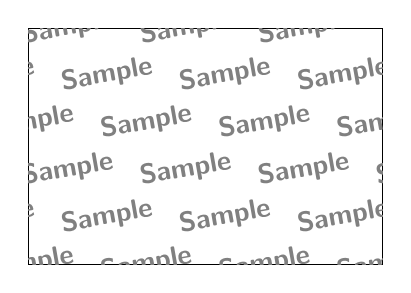
\begin{tikzpicture}
    \draw rectangle++(4.5,3);
    \clip rectangle++(4.5,3);
    \foreach\x in{0,1,2,3,4}{
      \foreach\y in{0,1,2,3,4,5,6}{
        \path(\x*1.5-\y*0.5,\y*0.6)node[rotate=10,text=gray]{\sffamily\bfseries\itshape Sample };
      }
    }
  \end{tikzpicture}
  %% 入れる画像：turtlesim を起動し、turtle_teleop_key でカメを少し動かして軌跡が描かれた状態のウィンドウのスクリーンショット
  % eps 画像を貼る場合は includegraphics をお使いください。
  % 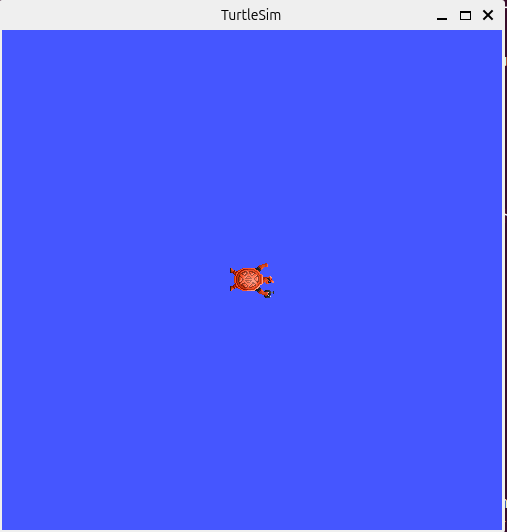
\includegraphics[width=0.6\linewidth]{ros2_install/turtlesim.png}
  \caption{turtlesim のウィンドウ}
  \label{fig:ros2-install-turtlesim}
\end{figure}

\subsection{キーボードでカメを動かす}

\key{Ctrl}+\key{Shift}+\key{T} で、ターミナルに新しいタブを開きます（\key{Ctrl}+\key{Alt}+\key{T} で新しいウィンドウを開いても構いません）。
新しいタブで、キーボードの入力を受け付けるノードを起動します。

\begin{terminal}[キーボードで操作するノードを起動する]
$ ros2 run turtlesim turtle_teleop_key
Reading from keyboard
---------------------------
Use arrow keys to move the turtle.
...
'Q' to quit.
\end{terminal}

このターミナルを選んだ状態で矢印キーを押すと、turtlesim のウィンドウの中のカメが動き、通った跡に線が描かれます。
カメが動かないときは、このターミナルのウィンドウがアクティブになっている（クリックして選ばれている）かを確かめてください。

\subsection{何が起きているのか}

このとき、2 つのノードが、ROS 2 の通信を使ってデータをやり取りしています（図\ref{fig:ros2-install-graph}）。

\begin{figure}[tb]
  \centering
  % 図：turtlesim のノードとトピック（chapters/ros2/ros2_install.tex）
\begin{tikzpicture}[
    node/.style={draw, ellipse, align=center, font=\small, fill=blue!8, minimum height=10mm, inner sep=2pt},
    topic/.style={draw, rectangle, font=\footnotesize\ttfamily, fill=orange!10, inner sep=3pt}]
  \node[node] (teleop) at (0,0) {\texttt{/teleop\_turtle}\\{\footnotesize キー入力}};
  \node[topic] (cmd) at (4.9,0) {/turtle1/cmd\_vel};
  \node[node] (sim) at (9.2,0) {\texttt{/turtlesim}\\{\footnotesize カメの画面}};
  \draw[figarrow] (teleop) -- node[figlabel, above]{速度の指令} (cmd);
  \draw[figarrow] (cmd) -- (sim);
  \node[figlabel, text=black!60, below=3mm of teleop] {ノード（楕円）};
  \node[figlabel, text=black!60, below=3mm of cmd] {トピック（四角）};
\end{tikzpicture}

  \caption{turtlesim を動かしているときのノードとトピック}
  \label{fig:ros2-install-graph}
\end{figure}

キーボードの入力を受け付ける \cmd{/teleop\_turtle} というノードが、押されたキーに応じた速度の指令を、\cmd{/turtle1/cmd\_vel} という名前の\textbf{トピック}に送っています。
カメの画面を表示する \cmd{/turtlesim} というノードが、そのトピックから指令を受け取って、カメを動かしています。
さらに別のタブを開いて、動いているノードとトピックの一覧を確かめてみましょう。

\begin{terminal}[ノードとトピックの一覧を確認する]
$ ros2 node list
/teleop_turtle
/turtlesim
$ ros2 topic list
/parameter_events
/rosout
/turtle1/cmd_vel
/turtle1/color_sensor
/turtle1/pose
\end{terminal}

ノードやトピックについては、次の\ref{chap:ros2_concepts}章で詳しく学びます。
確認が終わったら、それぞれのターミナルで \key{Ctrl}+\key{C} を押してノードを止めます（\cmd{turtle\_teleop\_key} は \key{q} でも終了できます）。

\subsection{デモのノードで通信を確かめる}

もう 1 つ、メッセージを送るノードと受け取るノードのデモでも試してみましょう。
2 つのターミナルで、それぞれ次のコマンドを実行します。

\begin{terminal}[1 つ目のターミナル：メッセージを送るノード]
$ ros2 run demo_nodes_cpp talker
[INFO] [1727930100.123456789] [talker]: Publishing: 'Hello World: 1'
[INFO] [1727930101.123456789] [talker]: Publishing: 'Hello World: 2'
...
\end{terminal}

\begin{terminal}[2 つ目のターミナル：メッセージを受け取るノード]
$ ros2 run demo_nodes_py listener
[INFO] [1727930102.234567890] [listener]: I heard: [Hello World: 3]
...
\end{terminal}

\cmd{talker} は C++ で、\cmd{listener} は Python で書かれたノードです。
書かれた言語が違っても、ROS 2 のノードどうしは同じように通信できることがわかります（\ref{sec:python-pros-cons}節のポイント）。

\section{ROS\_DOMAIN\_ID とネットワーク設定}
\label{sec:ros2-install-network}

\subsection{同じネットワークのノードは自動でつながる}

\ref{sec:what-is-ros-architecture}節で説明したように、ROS 2 では、同じネットワークにつながっているコンピュータのノードどうしが、自動でお互いを見つけて通信します。
これは便利な反面、研究室や競技会場のように、同じネットワークに複数の人のロボットや PC がある環境では困ったことになります。
自分のノードが、隣の人のロボットのトピックを受け取ってしまったり、自分の指令で隣の人のロボットが動いてしまったりするからです。

\subsection{ROS\_DOMAIN\_ID で通信を分ける}

このような混乱を防ぐのが、\textbf{\cmd{ROS\_DOMAIN\_ID}} という環境変数です。
\cmd{ROS\_DOMAIN\_ID} には 0 から 101 までの番号を設定でき、\textbf{同じ番号のノードどうしだけが通信します}。
番号を設定しなかった場合は 0 が使われます。

\begin{terminal}[ROS\_DOMAIN\_ID を設定する]
$ export ROS_DOMAIN_ID=12
\end{terminal}

\cmd{export} で設定した値は、そのターミナルだけで有効です（\ref{sec:env-export-source}節）。
いつも同じ番号を使うなら、\cmd{.bashrc} に追加しておきます。

\begin{terminal}[.bashrc に ROS\_DOMAIN\_ID を追加する]
$ echo "export ROS_DOMAIN_ID=12" >> ~/.bashrc
\end{terminal}

\begin{point}[ROS\_DOMAIN\_ID の決め方]
  研究室やチームの中で、人やロボットごとに重ならない番号を割り当てておきましょう。
  開発用 PC とロボットの PC で通信させたいときは、両方に同じ番号を設定します。
  「ノードが見えない」「トピックが届かない」というトラブルの原因として、\cmd{ROS\_DOMAIN\_ID} の設定の食い違いはとてもよくあります（\ref{chap:debug}章）。
  うまく通信できないときは、まず両方のターミナルで \cmd{echo \$ROS\_DOMAIN\_ID} を実行して、番号が同じかを確かめましょう。
\end{point}

\subsection{自分のコンピュータの中だけで通信する}

ほかのコンピュータとは一切通信せず、自分のコンピュータの中のノードどうしだけで通信したいときは、\cmd{ROS\_AUTOMATIC\_DISCOVERY\_RANGE} という環境変数に \cmd{LOCALHOST} を設定します。
シミュレータだけで学習しているときなどに便利です。

\begin{terminal}[自分のコンピュータの中だけで通信する]
$ export ROS_AUTOMATIC_DISCOVERY_RANGE=LOCALHOST
\end{terminal}

古い資料には \cmd{ROS\_LOCALHOST\_ONLY=1} という設定が書かれていることがありますが、ROS 2 Jazzy では \cmd{ROS\_AUTOMATIC\_DISCOVERY\_RANGE} を使います。

\subsection{別のコンピュータと通信するときの注意}

開発用 PC とロボットの PC のように、別々のコンピュータのノードどうしを通信させるには、次の点を確かめておきましょう。

\begin{itemize}
  \item 2 台のコンピュータが同じネットワークにつながっていて、\cmd{ping}（\ref{sec:network-check}節）で通信できること
  \item 両方の \cmd{ROS\_DOMAIN\_ID} が同じであること
  \item VirtualBox の仮想マシンを使っている場合は、ネットワークの設定が「ブリッジアダプター」になっていること（\ref{sec:linux-setup}節）。標準の NAT のままでは、ほかのコンピュータのノードを見つけられません
\end{itemize}

準備ができたら、片方のコンピュータで \cmd{talker}、もう片方で \cmd{listener} を起動して、メッセージが届くかを確かめてみましょう。
届かない場合は、ネットワークがノードを見つけるための通信（マルチキャスト）に対応しているかを、\cmd{ros2 multicast} コマンドで確かめられます。

\begin{terminal}[2 台のコンピュータの間でマルチキャストを確かめる]
$ ros2 multicast receive          # 1 台目：受信を待つ
$ ros2 multicast send             # 2 台目：送信する
\end{terminal}

1 台目に \cmd{Received from ...} と表示されれば、マルチキャストで通信できています。
Wi-Fi のルータによっては、マルチキャストの通信がうまく届かないことがあります。

\section*{この章のまとめ}

\begin{itemize}
  \item ROS 2 Jazzy は、ROS 2 のリポジトリを追加してから、apt で \cmd{ros-jazzy-desktop} と \cmd{ros-dev-tools} をインストールします。手順は公式ドキュメントも確認しましょう。
  \item ROS 2 を使うには、\cmd{source /opt/ros/jazzy/setup.bash} で設定を読み込みます。\cmd{.bashrc} に書いておくと、ターミナルを開くたびに自動で読み込まれます。
  \item \cmd{ros2 run パッケージ名 実行ファイル名} でノードを起動します。turtlesim で、ノードどうしがトピックで通信する様子を確かめました。
  \item 同じ \cmd{ROS\_DOMAIN\_ID} のノードどうしだけが通信します。人やロボットごとに番号を分け、通信させたいコンピュータどうしは同じ番号にそろえます。
\end{itemize}

\chapter{ROS 2 の基本概念とコマンドラインツール}
\label{chap:ros2_concepts}

% この章で学ぶこと
\begin{goalbox}
  \begin{itemize}
    \item ROS 2 のプログラムの単位であるノード
    \item ノードどうしの通信の方法（トピック・サービス・アクション）と、その使い分け
    \item やり取りするデータの型（メッセージ型）の調べ方
    \item ノードの設定値であるパラメータ
    \item \cmd{ros2} コマンドと rqt を使って、動いている ROS 2 のシステムを調べる方法
  \end{itemize}
\end{goalbox}

\ref{chap:ros2_install}章では、turtlesim を動かして、ROS 2 のノードどうしが通信する様子を少しだけ見ました。
この章では、ROS 2 の基本となる考え方を、turtlesim を使いながら 1 つずつ学びます。
あわせて、動いている ROS 2 のシステムの中をのぞくための \cmd{ros2} コマンドの使い方を身につけます。
これらのコマンドは、自分でノードを書くようになってからも、動作の確認やトラブルの調査で毎日のように使います。

この章では、次の 2 つのノードを起動した状態で進めます。
それぞれ別のターミナル（またはタブ）で起動し、そのままにしておいてください。

\begin{terminal}[1 つ目のターミナル：turtlesim]
$ ros2 run turtlesim turtlesim_node
\end{terminal}

\begin{terminal}[2 つ目のターミナル：キーボード操作]
$ ros2 run turtlesim turtle_teleop_key
\end{terminal}

以降のコマンドは、3 つ目のターミナルで実行します。

\section{ノード}
\label{sec:ros2-concepts-node}

\subsection{ノードとは}

\textbf{ノード}は、ROS 2 のプログラムの単位です。
\ref{sec:what-is-ros-components}節で見たように、ロボットのソフトウェアは、「センサのデータを読む」「地図を作る」「モータを動かす」といった、1 つの役割を持つノードの集まりとして作ります。
基本的には、1 つのノードが 1 つのプロセス（\ref{sec:linux-internals-process}節）として動きます。

\subsection{ノードを調べる}

動いているノードの一覧は、\cmd{ros2 node list} で表示できます。

\begin{terminal}[ノードの一覧を表示する]
$ ros2 node list
/teleop_turtle
/turtlesim
\end{terminal}

ノードの名前は \cmd{/} から始まります。
\cmd{ros2 node info} を使うと、そのノードがどのトピックやサービスを使っているかがわかります。

\begin{terminal}[ノードの詳しい情報を表示する]
$ ros2 node info /turtlesim
/turtlesim
  Subscribers:
    /parameter_events: rcl_interfaces/msg/ParameterEvent
    /turtle1/cmd_vel: geometry_msgs/msg/Twist
  Publishers:
    /parameter_events: rcl_interfaces/msg/ParameterEvent
    /rosout: rcl_interfaces/msg/Log
    /turtle1/color_sensor: turtlesim/msg/Color
    /turtle1/pose: turtlesim/msg/Pose
  Service Servers:
    /clear: std_srvs/srv/Empty
    /kill: turtlesim/srv/Kill
    /reset: std_srvs/srv/Empty
    /spawn: turtlesim/srv/Spawn
    ...
  Action Servers:
    /turtle1/rotate_absolute: turtlesim/action/RotateAbsolute
  ...
\end{terminal}

\cmd{Subscribers} や \cmd{Publishers} などの意味は、この後の節で順に説明します。

\subsection{ノードの名前を変えて起動する}

同じノードを、別の名前で起動することもできます。
\cmd{ros2 run} の後ろに \cmd{--ros-args --remap \_\_node:=名前} を付けると、ノードの名前を変えられます。

\begin{terminal}[ノードの名前を変えて起動する]
$ ros2 run turtlesim turtlesim_node --ros-args --remap __node:=my_turtle
\end{terminal}

別のターミナルで \cmd{ros2 node list} を実行すると、\cmd{/my\_turtle} というノードが増えていることがわかります。
このように、起動するときの名前や設定を変える方法は、\ref{chap:launch}章で詳しく学びます。
確認したら、\key{Ctrl}+\key{C} で止めておきましょう。

\section{トピック}
\label{sec:ros2-concepts-topic}

\subsection{ノードどうしの 3 つの通信方法}

ROS 2 のノードどうしは、主に\textbf{トピック}・\textbf{サービス}・\textbf{アクション}の 3 つの方法で通信します（図\ref{fig:ros2-concepts-communication}）。
それぞれ得意な場面が違うので、目的に合わせて使い分けます。

\begin{figure}[tb]
  \centering
  % 図：トピック・サービス・アクションの通信の違い（chapters/ros2/ros2_concepts.tex）
\begin{tikzpicture}[
    node/.style={draw, ellipse, font=\footnotesize, fill=blue!8, minimum width=20mm, minimum height=8mm, inner sep=1pt},
    lab/.style={font=\small\bfseries, anchor=west},
    msg/.style={font=\scriptsize, midway, fill=white, inner sep=1pt}]
  % トピック
  \node[lab] at (-1.2,0.9) {トピック（出版・購読）};
  \node[node] (p) at (0,0) {パブリッシャ};
  \node[draw, fill=orange!10, font=\scriptsize\ttfamily, inner sep=3pt] (t) at (4.4,0) {/scan};
  \node[node] (s1) at (7.4,0.45) {サブスクライバ};
  \node[node] (s2) at (7.4,-0.45) {サブスクライバ};
  \draw[figarrow] (p) -- node[msg, above=1pt]{データを送り続ける} (t);
  \draw[figarrow] (t) -- (s1.west);
  \draw[figarrow] (t) -- (s2.west);
  % サービス
  \node[lab] at (-1.2,-1.5) {サービス（要求・応答）};
  \node[node] (c) at (0,-2.4) {クライアント};
  \node[node] (sv) at (7.4,-2.4) {サーバ};
  \draw[figarrow] ([yshift=1.5mm]c.east) -- node[msg, above=1pt]{要求（リクエスト）} ([yshift=1.5mm]sv.west);
  \draw[figarrow] ([yshift=-1.5mm]sv.west) -- node[msg, below=1pt]{応答（レスポンス）を 1 回返す} ([yshift=-1.5mm]c.east);
  % アクション
  \node[lab] at (-1.2,-3.9) {アクション（目標・途中経過・結果）};
  \node[node] (ac) at (0,-5.1) {クライアント};
  \node[node] (as) at (7.4,-5.1) {サーバ};
  \draw[figarrow] ([yshift=3mm]ac.east) -- node[msg, above=1pt]{目標（ゴール）} ([yshift=3mm]as.west);
  \draw[figarrow, dashed] (as.west) -- node[msg]{途中経過（フィードバック）を何度も} (ac.east);
  \draw[figarrow] ([yshift=-3mm]as.west) -- node[msg, below=1pt]{結果（リザルト）} ([yshift=-3mm]ac.east);
\end{tikzpicture}

  \caption{トピック・サービス・アクションの通信の違い}
  \label{fig:ros2-concepts-communication}
\end{figure}

\subsection{トピックとは}

\textbf{トピック}は、データを流すための名前の付いた通り道です。
データを送るノードを\textbf{パブリッシャ}（出版者）、受け取るノードを\textbf{サブスクライバ}（購読者）といいます。
パブリッシャがトピックにデータを\textbf{パブリッシュ}（出版）すると、そのトピックを\textbf{サブスクライブ}（購読）しているすべてのノードにデータが届きます。

雑誌の出版と購読にたとえるとわかりやすいでしょう。
出版社は、誰が読んでいるかを気にせずに雑誌を出版し続け、購読者は、購読している雑誌が届くのを待ちます。
同じように、パブリッシャとサブスクライバは、お互いのことを知らなくても、トピックの名前さえ同じなら通信できます。
1 つのトピックに、複数のパブリッシャやサブスクライバがいても構いません。

トピックは、センサのデータやロボットへの速度の指令のように、\textbf{次々と流れ続けるデータ}を送るのに向いています。
ROS 2 の通信の中で、最もよく使われる方法です。

\subsection{トピックを調べる}

トピックの一覧は、\cmd{ros2 topic list} で表示できます。
\cmd{-t} を付けると、トピックに流れるデータの型（メッセージ型）も表示されます。

\begin{terminal}[トピックの一覧を表示する]
$ ros2 topic list -t
/parameter_events [rcl_interfaces/msg/ParameterEvent]
/rosout [rcl_interfaces/msg/Log]
/turtle1/cmd_vel [geometry_msgs/msg/Twist]
/turtle1/color_sensor [turtlesim/msg/Color]
/turtle1/pose [turtlesim/msg/Pose]
\end{terminal}

\cmd{/turtle1/cmd\_vel} はカメへの速度の指令、\cmd{/turtle1/pose} はカメの今の位置と向きを流すトピックです。
\cmd{/parameter\_events} と \cmd{/rosout} は、ROS 2 が自動で用意するトピックです。

\cmd{ros2 topic echo} を使うと、トピックに流れているデータをそのまま表示できます。

\begin{terminal}[トピックに流れるデータを表示する]
$ ros2 topic echo /turtle1/pose
x: 5.544444561004639
y: 5.544444561004639
theta: 0.0
linear_velocity: 0.0
angular_velocity: 0.0
---
...
\end{terminal}

2 つ目のターミナル（\cmd{turtle\_teleop\_key}）で矢印キーを押してカメを動かすと、表示される値が変わることがわかります。
止めるときは \key{Ctrl}+\key{C} を押します。

\cmd{ros2 topic info} でそのトピックのパブリッシャとサブスクライバの数を、\cmd{ros2 topic hz} でデータが 1 秒間に何回届いているかを調べられます。

\begin{terminal}[トピックの情報と頻度を調べる]
$ ros2 topic info /turtle1/cmd_vel
Type: geometry_msgs/msg/Twist
Publisher count: 1
Subscription count: 1
$ ros2 topic hz /turtle1/pose
average rate: 62.502
	min: 0.015s max: 0.017s std dev: 0.00041s window: 64
...
\end{terminal}

\subsection{メッセージ型}

トピックに流れるデータには、決まった形があります。
これを\textbf{メッセージ型}といい、\cmd{パッケージ名/msg/型の名前} の形で表します。
たとえば、\cmd{/turtle1/cmd\_vel} のメッセージ型は \cmd{geometry\_msgs/msg/Twist} です。
メッセージ型の中身は、\cmd{ros2 interface show} で確かめられます。

\begin{terminal}[メッセージ型の中身を表示する]
$ ros2 interface show geometry_msgs/msg/Twist
# This expresses velocity in free space broken into its linear and angular parts.

Vector3  linear
        float64 x
        float64 y
        float64 z
Vector3  angular
        float64 x
        float64 y
        float64 z
\end{terminal}

\cmd{Twist} は、並進の速度（\cmd{linear}）と回転の速度（\cmd{angular}）を、それぞれ x・y・z の 3 つの値で表すメッセージ型です。
平面を移動するロボットでは、\cmd{linear.x}（前後の速度 [m/s]）と \cmd{angular.z}（その場での回転の速度 [rad/s]）を主に使います。
\cmd{float64} は 64 ビットの小数を表す型です。

ロボット開発では、次のようなメッセージ型がよく使われます。

\begin{tablebox}[ロボット開発でよく使うメッセージ型][tab:ros2-concepts-msgs]
  \begin{tabular}{lp{0.5\linewidth}}
    \toprule
    メッセージ型 & 内容 \\
    \midrule
    \cmd{std\_msgs/msg/String} & 文字列 \\
    \cmd{geometry\_msgs/msg/Twist} & 速度（移動ロボットへの指令など） \\
    \cmd{sensor\_msgs/msg/LaserScan} & LiDAR で測った距離のデータ \\
    \cmd{sensor\_msgs/msg/Image} & カメラの画像 \\
    \cmd{sensor\_msgs/msg/Imu} & IMU の加速度・角速度 \\
    \cmd{nav\_msgs/msg/Odometry} & 車輪の回転などから推定したロボットの位置と速度 \\
    \bottomrule
  \end{tabular}
\end{tablebox}

\subsection{コマンドからトピックにパブリッシュする}

\cmd{ros2 topic pub} を使うと、コマンドからトピックにデータをパブリッシュできます。
自分でノードを書かなくても、ほかのノードの動作を試せるので便利です。
データの中身は、YAML という形式（\cmd{\{キー: 値\}}）で書きます。

\begin{terminal}[カメに速度の指令を 1 回送る]
$ ros2 topic pub --once /turtle1/cmd_vel geometry_msgs/msg/Twist "{linear: {x: 2.0, y: 0.0, z: 0.0}, angular: {x: 0.0, y: 0.0, z: 1.8}}"
publisher: beginning loop
publishing #1: geometry_msgs.msg.Twist(linear=geometry_msgs.msg.Vector3(x=2.0, y=0.0, z=0.0), angular=geometry_msgs.msg.Vector3(x=0.0, y=0.0, z=1.8))
\end{terminal}

カメが少しだけ前に進みながら曲がります。
\cmd{--once} の代わりに \cmd{--rate 1} を付けると、1 秒に 1 回、止めるまで送り続けるので、カメは円を描いて動き続けます。

\begin{terminal}[カメに速度の指令を送り続ける]
$ ros2 topic pub --rate 1 /turtle1/cmd_vel geometry_msgs/msg/Twist "{linear: {x: 2.0}, angular: {z: 1.8}}"
\end{terminal}

省略した値は 0 になるので、このように必要な値だけを書いても構いません。
確認したら、\key{Ctrl}+\key{C} で止めましょう。

\section{サービス}
\label{sec:ros2-concepts-service}

\subsection{サービスとは}

\textbf{サービス}は、\textbf{要求（リクエスト）を送ると、応答（レスポンス）が 1 回返ってくる}通信の方法です。
サービスを提供するノードを\textbf{サーバ}、サービスを呼び出すノードを\textbf{クライアント}といいます。
お店での注文にたとえると、注文（リクエスト）をすると、品物（レスポンス）が渡されるような関係です。

トピックが「流れ続けるデータ」に向いているのに対して、サービスは「この処理をしてほしい」「この値を教えてほしい」といった、\textbf{1 回で終わるやり取り}に向いています。
ただし、クライアントは応答が返ってくるまで待つことになるので、時間のかかる処理には向いていません（その場合は、次の節のアクションを使います）。

\subsection{サービスを調べて呼び出す}

サービスの一覧は、\cmd{ros2 service list} で表示できます。
\cmd{-t} を付けると、サービスの型も表示されます。

\begin{terminal}[サービスの一覧を表示する]
$ ros2 service list -t
/clear [std_srvs/srv/Empty]
/kill [turtlesim/srv/Kill]
/reset [std_srvs/srv/Empty]
/spawn [turtlesim/srv/Spawn]
/turtle1/set_pen [turtlesim/srv/SetPen]
/turtle1/teleport_absolute [turtlesim/srv/TeleportAbsolute]
...
\end{terminal}

サービスの型の中身も、\cmd{ros2 interface show} で確かめられます。
\cmd{---} の上がリクエスト、下がレスポンスの形です。

\begin{terminal}[サービスの型の中身を表示する]
$ ros2 interface show turtlesim/srv/Spawn
float32 x
float32 y
float32 theta
string name # Optional.  A unique name will be created and returned if this is empty
---
string name
\end{terminal}

\cmd{/spawn} は、指定した位置に新しいカメを出すサービスです。
\cmd{ros2 service call} で、コマンドからサービスを呼び出してみましょう。

\begin{terminal}[新しいカメを出すサービスを呼び出す]
$ ros2 service call /spawn turtlesim/srv/Spawn "{x: 2.0, y: 2.0, theta: 0.2, name: ''}"
requester: making request: turtlesim.srv.Spawn_Request(x=2.0, y=2.0, theta=0.2, name='')

response:
turtlesim.srv.Spawn_Response(name='turtle2')
\end{terminal}

turtlesim のウィンドウに、2 匹目のカメが現れます。
レスポンスとして、新しいカメの名前（\cmd{turtle2}）が返ってきています。
ほかにも、\cmd{/clear}（カメの軌跡を消す）などのサービスを試してみましょう。

\begin{terminal}[カメの軌跡を消すサービスを呼び出す]
$ ros2 service call /clear std_srvs/srv/Empty
\end{terminal}

\section{アクション}
\label{sec:ros2-concepts-action}

\subsection{アクションとは}

\textbf{アクション}は、\textbf{時間のかかる処理}を頼むための通信の方法です。
クライアントがサーバに\textbf{目標（ゴール）}を送ると、サーバは処理を進めながら\textbf{途中経過（フィードバック）}を何度も送り返し、処理が終わったら\textbf{結果（リザルト）}を返します。
また、処理の途中で\textbf{キャンセル}することもできます。

たとえば、「目的地まで移動して」という指示を出すと、ロボットは移動しながら「残りあと 3 m」のように途中経過を知らせ、着いたら「到着した」と結果を返す、といった使い方です。
\ref{chap:practice}章で使う Navigation2 の自律移動も、アクションで指示を出します。

\subsection{アクションを調べて呼び出す}

アクションの一覧は、\cmd{ros2 action list} で表示できます。

\begin{terminal}[アクションの一覧を表示する]
$ ros2 action list -t
/turtle1/rotate_absolute [turtlesim/action/RotateAbsolute]
\end{terminal}

\cmd{/turtle1/rotate\_absolute} は、カメを指定した向きまで回転させるアクションです。
アクションの型は、\cmd{---} で区切られた 3 つの部分（ゴール・リザルト・フィードバック）でできています。

\begin{terminal}[アクションの型の中身を表示する]
$ ros2 interface show turtlesim/action/RotateAbsolute
# The desired heading in radians
float32 theta
---
# The angular displacement in radians to the starting position
float32 delta
---
# The remaining rotation in radians
float32 remaining
\end{terminal}

\cmd{ros2 action send\_goal} でゴールを送ってみましょう。
\cmd{--feedback} を付けると、途中経過も表示されます。
向き（\cmd{theta}）はラジアンで指定します（1.57 ラジアンは約 90 度です）。

\begin{terminal}[カメを回転させるアクションのゴールを送る]
$ ros2 action send_goal /turtle1/rotate_absolute turtlesim/action/RotateAbsolute "{theta: 1.57}" --feedback
Waiting for an action server to become available...
Sending goal:
     theta: 1.57

Goal accepted with ID: f8db8f44410849eaa93d3feb747dd444

Feedback:
    remaining: -1.5520000457763672
...
Result:
    delta: -1.5679999589920044

Goal finished with status: SUCCEEDED
\end{terminal}

カメがゆっくり回転し、その間、残りの回転量（\cmd{remaining}）がフィードバックとして届き、最後に結果が表示されます。
実は、\cmd{turtle\_teleop\_key} の \key{G} \key{B} \key{V} \key{C} \key{D} \key{E} \key{R} \key{T} キーも、このアクションを使ってカメの向きを変えています。

\subsection{通信の方法の使い分け}

3 つの通信の方法の違いを、表にまとめておきます。

\begin{tablebox}[トピック・サービス・アクションの使い分け][tab:ros2-concepts-compare]
  \begin{tabular}{lp{0.28\linewidth}p{0.4\linewidth}}
    \toprule
    方法 & やり取り & 向いている場面 \\
    \midrule
    トピック & 一方向に流し続ける & センサのデータ、速度の指令など、次々と流れるデータ \\
    サービス & 要求に対して 1 回応答する & 設定の変更や値の問い合わせなど、すぐに終わる処理 \\
    アクション & 目標・途中経過・結果。キャンセルもできる & 目的地への移動やアームの動作など、時間のかかる処理 \\
    \bottomrule
  \end{tabular}
\end{tablebox}

\section{パラメータ}
\label{sec:ros2-concepts-param}

\subsection{パラメータとは}

\textbf{パラメータ}は、ノードが持っている設定値です。
たとえば、ロボットの最高速度や、センサのデバイスファイルの名前（\cmd{/dev/ttyUSB0} など）を、プログラムに直接書き込むのではなくパラメータにしておけば、プログラムを書き換えずに、起動するときや実行中に設定を変えられます。
turtlesim のノードは、背景の色をパラメータとして持っています。

\subsection{パラメータを調べて変更する}

パラメータの一覧は、\cmd{ros2 param list} で表示できます。

\begin{terminal}[パラメータの一覧を表示する]
$ ros2 param list
/teleop_turtle:
  qos_overrides./parameter_events.publisher.depth
  ...
  scale_angular
  scale_linear
  use_sim_time
/turtlesim:
  background_b
  background_g
  background_r
  ...
  use_sim_time
\end{terminal}

\cmd{ros2 param get} でパラメータの値を表示し、\cmd{ros2 param set} で値を変更できます。

\begin{terminal}[パラメータの値を表示・変更する]
$ ros2 param get /turtlesim background_r
Integer value is: 69
$ ros2 param set /turtlesim background_r 150
Set parameter successful
\end{terminal}

turtlesim のウィンドウの背景の色が変わります。

\subsection{パラメータをファイルに保存する}

\cmd{ros2 param dump} を使うと、ノードのパラメータを YAML 形式で表示できます。
リダイレクト（\ref{sec:text-pipe-redirect}節）でファイルに保存しておけば、次にノードを起動するときに \cmd{--params-file} で読み込んで、同じ設定で起動できます。

\begin{terminal}[パラメータをファイルに保存して、起動時に読み込む]
$ ros2 param dump /turtlesim > turtlesim.yaml
$ ros2 run turtlesim turtlesim_node --ros-args --params-file turtlesim.yaml
\end{terminal}

パラメータをファイルで管理する方法は、\ref{chap:launch}章で詳しく学びます。

\section{rqt と rqt\_graph による可視化}
\label{sec:ros2-concepts-rqt}

\subsection{rqt\_graph}

ノードとトピックの数が増えてくると、コマンドの出力だけでは、全体のつながりがわかりにくくなります。
\textbf{rqt\_graph} を使うと、動いているノードとトピックのつながりを図で表示できます。

\begin{terminal}[rqt\_graph を起動する]
$ rqt_graph
\end{terminal}

\begin{figure}[tb]
  \centering
  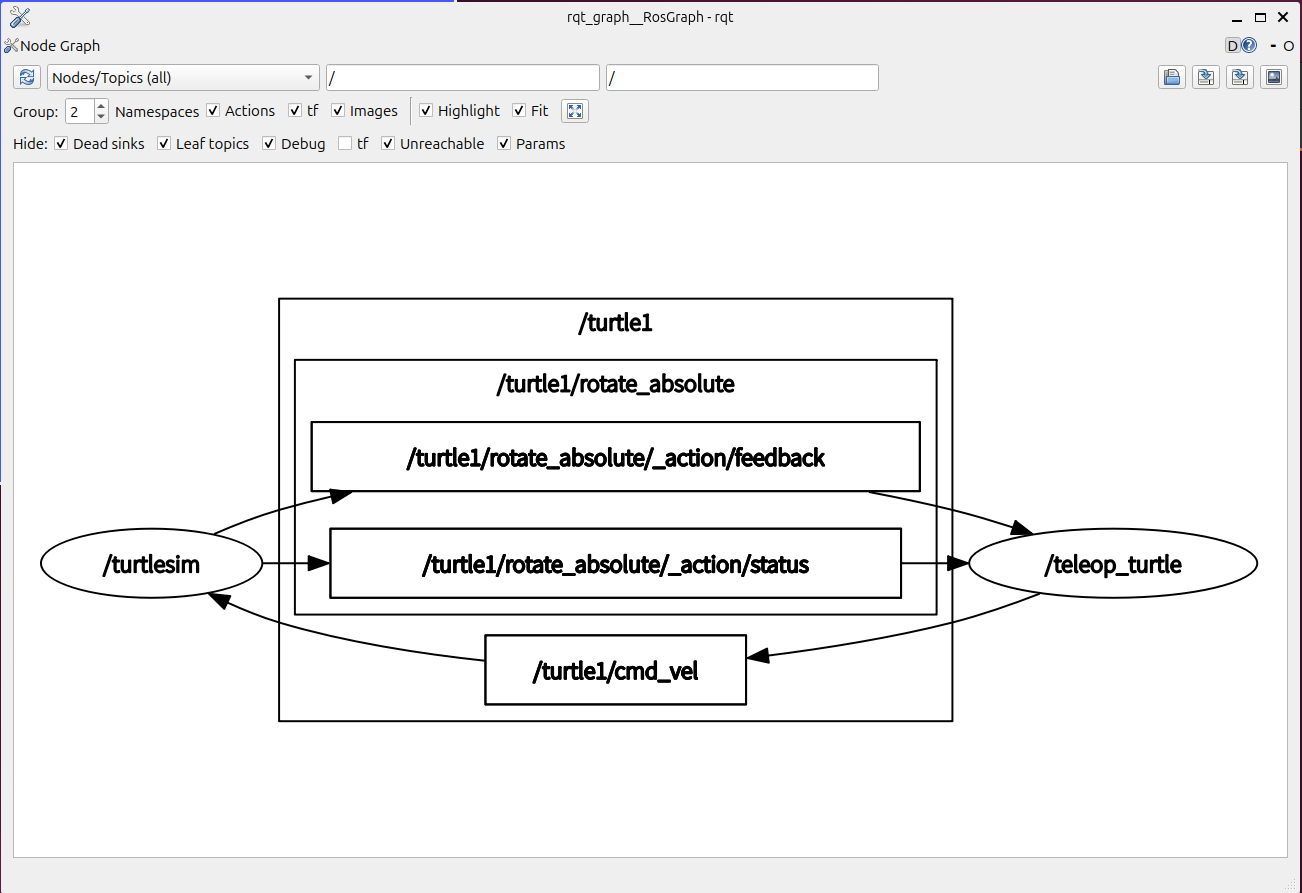
\includegraphics[width=0.9\linewidth]{ros2_concepts/rqt_graph.png}
  \caption{rqt\_graph でノードとトピックのつながりを表示した例}
  \label{fig:ros2-concepts-rqt-graph}
\end{figure}

図\ref{fig:ros2-concepts-rqt-graph}のように、楕円がノード、四角がトピックを表し、矢印がデータの流れる向きを表します。
\cmd{/teleop\_turtle} から \cmd{/turtlesim} へ、\cmd{/turtle1/cmd\_vel} トピックでデータが流れていることが一目でわかります。
\cmd{/turtle1/rotate\_absolute} の中の四角は、\ref{sec:ros2-concepts-action}節で学ぶアクションが内部で使っているトピックです。
自分で作ったノードが思ったとおりにつながっているかを確かめるときに、とても便利です。
表示が更新されないときは、左上の更新ボタンを押します。

\subsection{rqt}

\textbf{rqt} は、ROS 2 のさまざまな GUI のツールを、プラグインとしてまとめて使える道具です。
\cmd{rqt} コマンドで起動し、メニューの「Plugins」から使いたいツールを選びます。
rqt\_graph も、rqt のプラグインの 1 つです。

\begin{tablebox}[rqt のよく使うプラグイン][tab:ros2-concepts-rqt]
  \begin{tabular}{lp{0.55\linewidth}}
    \toprule
    プラグイン & できること \\
    \midrule
    Node Graph & ノードとトピックのつながりを表示する（rqt\_graph と同じ） \\
    Topic Monitor & トピックに流れているデータを一覧で表示する \\
    Message Publisher & GUI でトピックにデータをパブリッシュする \\
    Service Caller & GUI でサービスを呼び出す \\
    Plot & トピックの数値をグラフにする \\
    Console & ノードが出力したログを表示する（\ref{chap:debug}章） \\
    \bottomrule
  \end{tabular}
\end{tablebox}

\begin{point}[ros2 コマンドのまとめ]
  この章で使った \cmd{ros2} コマンドは、\cmd{ros2 対象 操作} という共通の形をしています。
  \begin{itemize}
    \item 対象：\cmd{node}, \cmd{topic}, \cmd{service}, \cmd{action}, \cmd{param}, \cmd{interface}
    \item 操作：\cmd{list}（一覧）、\cmd{info}（詳細）、\cmd{echo}（表示）、\cmd{pub}（送る）、\cmd{call}（呼び出す）、\cmd{get} / \cmd{set}（取得・変更）など
  \end{itemize}
  使い方を忘れたら、\cmd{ros2 topic --help} のように \cmd{--help} を付けて調べましょう（\ref{sec:terminal-help}節）。
\end{point}

\section*{この章のまとめ}

\begin{itemize}
  \item ノードは ROS 2 のプログラムの単位です。\cmd{ros2 node list} と \cmd{ros2 node info} で調べられます。
  \item トピックは、パブリッシャからサブスクライバへデータを流し続ける通信の方法です。\cmd{ros2 topic list} / \cmd{echo} / \cmd{pub} で調べたり、データを送ったりできます。データの形はメッセージ型で決まっていて、\cmd{ros2 interface show} で確かめられます。
  \item サービスは要求に対して 1 回応答する通信、アクションは時間のかかる処理を頼み、途中経過と結果を受け取る通信です。
  \item パラメータはノードの設定値で、\cmd{ros2 param get} / \cmd{set} で表示・変更できます。
  \item rqt\_graph でノードとトピックのつながりを図で確かめられます。rqt には、ほかにも便利なプラグインがあります。
\end{itemize}

\chapter{ワークスペースとパッケージ}
\label{chap:workspace}

% この章で学ぶこと
\begin{goalbox}
  \begin{itemize}
    \item ROS 2 のワークスペースの構成（\cmd{src}, \cmd{build}, \cmd{install}, \cmd{log}）
    \item colcon を使ったパッケージのビルド
    \item \cmd{ros2 pkg create} による自分のパッケージの作成
    \item \cmd{package.xml} と \cmd{setup.py}（\cmd{CMakeLists.txt}）の役割
    \item rosdep による依存関係の解決
    \item オーバーレイとアンダーレイの考え方
  \end{itemize}
\end{goalbox}

ここまでは、apt でインストールした ROS 2 のパッケージ（turtlesim など）を使ってきました。
自分でノードを書いたり、公開されているパッケージをソースコードからビルドしたりするには、\textbf{ワークスペース}という作業場所を用意します。
この章では、ワークスペースの作り方と、パッケージの作り方・ビルドの仕方を学びます。
次の\ref{chap:rclpy}章からは、ここで作ったワークスペースとパッケージを使って、Python でノードを書いていきます。

\section{ワークスペースの構成}
\label{sec:workspace-structure}

\subsection{パッケージとワークスペース}

ROS 2 では、ノードのプログラムや設定ファイルなどを、\textbf{パッケージ}という単位でまとめます（\ref{sec:what-is-ros-components}節）。
turtlesim も、\cmd{turtlesim} という名前のパッケージです。
1 つのパッケージには、関係する複数のノードや、ノードの設定ファイル、起動用のファイル（\ref{chap:launch}章）などを入れられます。

\textbf{ワークスペース}は、パッケージのソースコードを置き、ビルドするためのディレクトリです。
ワークスペースの名前は自由ですが、\cmd{\textasciitilde/ros2\_ws} とするのが一般的です。

\subsection{ワークスペースを作る}

ワークスペースを作るには、ワークスペースのディレクトリと、その中に \cmd{src} ディレクトリを作るだけです（\ref{sec:files-manipulate}節の \cmd{mkdir -p}）。

\begin{terminal}[ワークスペースを作る]
$ mkdir -p ~/ros2_ws/src
$ cd ~/ros2_ws
\end{terminal}

パッケージのソースコードは、すべて \cmd{src} ディレクトリの中に置きます。
ワークスペースでビルドを行うと、\cmd{src} と同じ階層に、自動で 3 つのディレクトリが作られます。

\begin{tablebox}[ワークスペースのディレクトリ][tab:workspace-dirs]
  \begin{tabular}{lp{0.6\linewidth}}
    \toprule
    ディレクトリ & 役割 \\
    \midrule
    \cmd{src} & パッケージのソースコードを置く。自分で編集するのはここだけ \\
    \cmd{build} & ビルドの途中で作られるファイルが置かれる \\
    \cmd{install} & ビルドしてできたものがインストールされる。ノードはここから実行される \\
    \cmd{log} & ビルドのログが置かれる \\
    \bottomrule
  \end{tabular}
\end{tablebox}

\cmd{build}・\cmd{install}・\cmd{log} は、ビルドのたびに作り直されるディレクトリです。
自分で編集する必要はなく、Git で管理するときも含めません（\ref{sec:git-basic}節の \cmd{.gitignore}）。
ビルドがおかしくなったときは、この 3 つのディレクトリを \cmd{rm -r} で削除してから、ビルドし直すと直ることがあります。

\section{colcon によるビルド}
\label{sec:workspace-colcon}

\subsection{colcon}

ROS 2 では、\textbf{colcon}（コルコン）というツールで、ワークスペースの中のパッケージをまとめてビルドします。
colcon は、\ref{sec:ros2-install-install}節でインストールした \cmd{ros-dev-tools} に含まれています。
colcon は、パッケージどうしの依存関係を調べて、正しい順番でビルドしてくれます。
C++ のパッケージは、内部で CMake（\ref{sec:package-build}節）を使ってビルドされます。

\subsection{公開されているパッケージをビルドする}

試しに、turtlesim のソースコードをダウンロードして、自分のワークスペースでビルドしてみましょう。
turtlesim のソースコードは、\cmd{ros\_tutorials} というリポジトリで公開されています。
\cmd{git clone}（\ref{sec:git-github}節）で、Jazzy 用のブランチ（\cmd{-b jazzy}）をダウンロードします。

\begin{terminal}[turtlesim のソースコードをダウンロードする]
$ cd ~/ros2_ws/src
$ git clone https://github.com/ros/ros_tutorials.git -b jazzy
\end{terminal}

ビルドする前に、パッケージが必要としている依存パッケージをインストールしておきます（詳しくは\ref{sec:workspace-rosdep}節で説明します）。

\begin{terminal}[依存パッケージをインストールする]
$ cd ~/ros2_ws
$ sudo rosdep init        # 最初の 1 回だけ
$ rosdep update
$ rosdep install -i --from-path src --rosdistro jazzy -y
#All required rosdeps installed successfully
\end{terminal}

準備ができたら、\textbf{ワークスペースのディレクトリ}（\cmd{\textasciitilde/ros2\_ws}）で \cmd{colcon build} を実行します。

\begin{terminal}[ワークスペースをビルドする]
$ cd ~/ros2_ws
$ colcon build
Starting >>> turtlesim
Finished <<< turtlesim [25.2s]

Summary: 1 package finished [25.6s]
\end{terminal}

\cmd{Summary} に、ビルドに成功したパッケージの数が表示されます。
ワークスペースの中を見ると、\cmd{build}・\cmd{install}・\cmd{log} ができています。

\begin{terminal}[ビルド後のワークスペース]
$ ls
build  install  log  src
\end{terminal}

\begin{caution}[colcon build はワークスペースのディレクトリで]
  \cmd{colcon build} は、必ずワークスペースのディレクトリ（\cmd{src} の 1 つ上）で実行します。
  \cmd{src} の中や、パッケージのディレクトリの中で実行すると、その場所に \cmd{build} などのディレクトリが作られてしまい、混乱の原因になります。
  間違えて作ってしまったら、そのディレクトリを削除しましょう。
\end{caution}

\subsection{colcon build のよく使うオプション}

\begin{tablebox}[\cmd{colcon build} のよく使うオプション][tab:workspace-colcon-options]
  \begin{tabular}{p{0.42\linewidth}p{0.5\linewidth}}
    \toprule
    オプション & 意味 \\
    \midrule
    \cmd{--packages-select パッケージ名} & 指定したパッケージだけをビルドする \\
    \cmd{--packages-up-to パッケージ名} & 指定したパッケージと、それが依存するパッケージをビルドする \\
    \cmd{--symlink-install} & ファイルをコピーせずにリンクでインストールする。Python のファイルなどを書き換えたとき、ビルドし直さずに反映される \\
    \bottomrule
  \end{tabular}
\end{tablebox}

パッケージが増えてくると、ビルドに時間がかかるようになります。
変更したパッケージだけを \cmd{--packages-select} でビルドすると、時間を短くできます。
Python のノードを書くときは、\cmd{--symlink-install} を付けておくと便利です（\ref{chap:rclpy}章）。
よく使うので、\ref{sec:env-alias}節で紹介したように、エイリアスを作っておくのもよいでしょう。

\section{パッケージの作成}
\label{sec:workspace-create}

\subsection{ros2 pkg create}

自分のパッケージは、\cmd{ros2 pkg create} コマンドで作ります。
パッケージのひな形となるディレクトリやファイルを、自動で作ってくれます。
パッケージは、ワークスペースの \cmd{src} ディレクトリの中に作ります。

\begin{terminal}[Python のパッケージを作る]
$ cd ~/ros2_ws/src
$ ros2 pkg create --build-type ament_python --license Apache-2.0 --node-name my_node my_package
going to create a new package
package name: my_package
destination directory: /home/user/ros2_ws/src
...
\end{terminal}

\begin{description}
  \item[\cmd{--build-type ament\_python}] Python でノードを書くパッケージを作ります。C++ の場合は \cmd{ament\_cmake} を指定します。
  \item[\cmd{--license Apache-2.0}] パッケージのライセンスを指定します（\ref{sec:linux-oss}節）。
  \item[\cmd{--node-name my\_node}] 指定した名前で、ノードのひな形のファイルも作ります。
  \item[\cmd{my\_package}] パッケージの名前です。パッケージ名には、小文字の英数字とアンダースコアを使います。
\end{description}

ほかのパッケージを使うノードを書く場合は、\cmd{--dependencies rclpy std\_msgs} のように、依存するパッケージも指定できます。

\subsection{パッケージの中身}

作られたパッケージの中を、\cmd{tree} コマンド（\ref{sec:package-apt}節）で見てみましょう。

\begin{terminal}[Python のパッケージの中身]
$ tree my_package
my_package
├── my_package
│   ├── __init__.py
│   └── my_node.py
├── package.xml
├── resource
│   └── my_package
├── setup.cfg
├── setup.py
└── test
    ├── test_copyright.py
    ├── test_flake8.py
    └── test_pep257.py
\end{terminal}

\begin{description}
  \item[\cmd{my\_package/}] パッケージと同じ名前のディレクトリで、ここに Python のノードのファイルを置きます。\cmd{\_\_init\_\_.py} は、このディレクトリを Python のモジュール（\ref{sec:python-class-module}節）として扱うための空のファイルです。
  \item[\cmd{package.xml}] パッケージの情報を書くファイルです（\ref{sec:workspace-files}節）。
  \item[\cmd{setup.py}, \cmd{setup.cfg}] Python のパッケージのインストール方法を書くファイルです。
  \item[\cmd{resource/}] ROS 2 がパッケージを見つけるための目印のファイルが入っています。
  \item[\cmd{test/}] コードの書き方を自動で確かめるテストが入っています。
\end{description}

\cmd{my\_node.py} には、次のようなひな形が書かれています。
\ref{sec:python-class-module}節で学んだ \cmd{if \_\_name\_\_ == '\_\_main\_\_':} が使われていることがわかります。

\begin{lstlisting}[style=python, caption={ノードのひな形（my\_package/my\_package/my\_node.py）}, label={lst:workspace-my-node}]
def main():
    print('Hi from my_package.')


if __name__ == '__main__':
    main()
\end{lstlisting}

\subsection{ビルドして実行する}

作ったパッケージをビルドして、実行してみましょう。
ビルドしたパッケージを使うには、ワークスペースの \cmd{install/local\_setup.bash} を \cmd{source} で読み込む必要があります（\ref{sec:workspace-overlay}節）。

\begin{terminal}[パッケージをビルドして実行する]
$ cd ~/ros2_ws
$ colcon build --packages-select my_package
Starting >>> my_package
Finished <<< my_package [1.21s]

Summary: 1 package finished [1.52s]
$ source install/local_setup.bash
$ ros2 run my_package my_node
Hi from my_package.
\end{terminal}

自分で作ったパッケージのノードを、\cmd{ros2 run} で実行できました。
まだ ROS 2 の通信は使っていませんが、次の\ref{chap:rclpy}章で、このパッケージにノードを書いていきます。

\section{package.xml と setup.py / CMakeLists.txt}
\label{sec:workspace-files}

\subsection{package.xml}

\cmd{package.xml} は、パッケージの名前・バージョン・説明・管理者・ライセンス、そして\textbf{依存するパッケージ}を書くファイルです。
XML（タグで囲んで書く形式）で書かれています。

\begin{lstlisting}[style=xml, caption={package.xml}, label={lst:workspace-package-xml}]
<?xml version="1.0"?>
<?xml-model href="http://download.ros.org/schema/package_format3.xsd" schematypens="http://www.w3.org/2001/XMLSchema"?>
<package format="3">
  <name>my_package</name>
  <version>0.0.0</version>
  <description>TODO: Package description</description>
  <maintainer email="user@todo.todo">user</maintainer>
  <license>Apache-2.0</license>

  <test_depend>ament_copyright</test_depend>
  <test_depend>ament_flake8</test_depend>
  <test_depend>ament_pep257</test_depend>
  <test_depend>python3-pytest</test_depend>

  <export>
    <build_type>ament_python</build_type>
  </export>
</package>
\end{lstlisting}

\cmd{description} や \cmd{maintainer} は、自分のパッケージの説明や、自分の名前とメールアドレスに書き換えておきましょう。
\cmd{license} には、\ref{sec:linux-oss}節で学んだライセンスを書きます。
パッケージを公開するときに、ほかの人が安心して使えるように、必ずライセンスを明記しておきましょう。

ほかのパッケージを使う場合は、そのパッケージ名を \cmd{<depend>} タグで書きます。
たとえば、\cmd{rclpy} と \cmd{std\_msgs} を使うノードを書くなら、次の 2 行を追加します。

\begin{lstlisting}[style=xml, caption={package.xml に依存するパッケージを追加する}, label={lst:workspace-depend}]
  <depend>rclpy</depend>
  <depend>std_msgs</depend>
\end{lstlisting}

ここに書いた依存関係をもとに、colcon はビルドの順番を決め、rosdep は必要なパッケージをインストールします（\ref{sec:workspace-rosdep}節）。

\subsection{setup.py}

Python のパッケージ（\cmd{ament\_python}）では、\cmd{setup.py} に、パッケージをどのようにインストールするかを書きます。
特に大切なのは、最後の \cmd{entry\_points} の部分です。

\begin{lstlisting}[style=python, caption={setup.py（一部）}, label={lst:workspace-setup-py}]
setup(
    name=package_name,
    ...
    license='Apache-2.0',
    entry_points={
        'console_scripts': [
            'my_node = my_package.my_node:main'
        ],
    },
)
\end{lstlisting}

\cmd{'my\_node = my\_package.my\_node:main'} は、「\cmd{ros2 run my\_package my\_node} と実行されたら、\cmd{my\_package} ディレクトリの \cmd{my\_node.py} の \cmd{main} 関数を呼び出す」という意味です。
新しいノードのファイルを追加したときは、ここに 1 行追加して、ビルドし直します（\ref{chap:rclpy}章）。

\subsection{CMakeLists.txt}

C++ のパッケージ（\cmd{ament\_cmake}）では、\cmd{setup.py} の代わりに \cmd{CMakeLists.txt}（\ref{sec:package-build}節）にビルドの方法を書きます。
C++ でノードを書く場合のほか、自分でメッセージ型を定義するパッケージ（\ref{chap:rclpy}章）でも使います。

\section{依存関係の解決}
\label{sec:workspace-rosdep}

\subsection{rosdep}

公開されているパッケージをソースコードからビルドするときは、そのパッケージが必要とするほかのパッケージ（依存パッケージ）を、先にインストールしておく必要があります。
一つ一つ調べて \cmd{apt install} するのは大変なので、ROS 2 では \textbf{rosdep} というツールを使います。

rosdep は、ワークスペースの中のパッケージの \cmd{package.xml} を読み、そこに書かれた依存パッケージを、apt のパッケージ名（\cmd{ros-jazzy-...} や \cmd{python3-...} など）に変換して、まとめてインストールしてくれます。
\ref{sec:python-pep668}節で説明したように、ROS 2 のノードで使う Python のパッケージも、rosdep を通じて apt でインストールされます。

\subsection{rosdep の使い方}

rosdep を初めて使うときは、最初に 1 回だけ \cmd{sudo rosdep init} を実行して、初期設定をします。
その後、\cmd{rosdep update} で、依存パッケージの対応表を最新にします。

\begin{terminal}[rosdep の初期設定と更新]
$ sudo rosdep init
$ rosdep update
\end{terminal}

依存パッケージをインストールするには、ワークスペースのディレクトリで次のコマンドを実行します。

\begin{terminal}[依存パッケージをインストールする]
$ cd ~/ros2_ws
$ rosdep install -i --from-path src --rosdistro jazzy -y
\end{terminal}

\begin{description}
  \item[\cmd{--from-path src}] \cmd{src} の中のすべてのパッケージの依存関係を調べる
  \item[\cmd{-i}] ワークスペースの中にあるパッケージは、インストールの対象から外す
  \item[\cmd{--rosdistro jazzy}] ROS 2 のディストリビューションを指定する
  \item[\cmd{-y}] インストールの確認に、自動で「はい」と答える
\end{description}

\begin{point}[ソースからビルドするときの手順]
  公開されているパッケージをソースコードからビルドするときは、次の流れが基本です。
  \begin{enumerate}
    \item \cmd{src} の中に \cmd{git clone} する
    \item ワークスペースのディレクトリで \cmd{rosdep install} を実行する
    \item \cmd{colcon build} でビルドする
    \item \cmd{source install/local\_setup.bash} で読み込む
  \end{enumerate}
  ただし、apt でインストールできるパッケージ（\cmd{ros-jazzy-...}）は、まず apt で入れることを考えましょう（\ref{sec:package-build}節の注意）。
\end{point}

\section{オーバーレイとアンダーレイ}
\label{sec:workspace-overlay}

\subsection{ワークスペースを重ねる}

ROS 2 では、ワークスペースを重ねて使います（図\ref{fig:workspace-overlay}）。
apt でインストールした ROS 2（\cmd{/opt/ros/jazzy}）の上に、自分のワークスペース（\cmd{\textasciitilde/ros2\_ws}）を重ねる、というイメージです。
下になる環境を\textbf{アンダーレイ}、上に重ねる環境を\textbf{オーバーレイ}といいます。

\begin{figure}[tb]
  \centering
  % 図：アンダーレイとオーバーレイ（chapters/ros2/workspace.tex）
\begin{tikzpicture}[ws/.style={draw, rounded corners=2pt, align=left, font=\small, text width=80mm, minimum height=14mm, inner sep=4pt, anchor=west}]
  \node[ws, fill=blue!8] (under) at (0,0) {\textbf{アンダーレイ}：\texttt{/opt/ros/jazzy}\\{\footnotesize apt でインストールした ROS 2（turtlesim、rclpy など）}};
  \node[ws, fill=green!10] (over) at (0,1.75) {\textbf{オーバーレイ}：\texttt{\textasciitilde/ros2\_ws/install}\\{\footnotesize 自分でビルドしたパッケージ（my\_package、改造した turtlesim など）}};
  \draw[figarrow] (8.9,-0.4) -- node[figlabel, right, align=left]{後から\\読み込む} (8.9,2.2);
  \node[figlabel, anchor=west, align=left, text=black!70] at (0,3.15) {同じ名前のパッケージがあるときは、オーバーレイ（上）のほうが使われる};
\end{tikzpicture}

  \caption{アンダーレイとオーバーレイ}
  \label{fig:workspace-overlay}
\end{figure}

ワークスペースを使うときは、まずアンダーレイ（ROS 2 本体）の設定を読み込み、その後にオーバーレイ（自分のワークスペース）の設定を読み込みます。

\begin{terminal}[アンダーレイとオーバーレイを読み込む]
$ source /opt/ros/jazzy/setup.bash          # アンダーレイ
$ source ~/ros2_ws/install/local_setup.bash # オーバーレイ
\end{terminal}

1 行目は、\ref{sec:ros2-install-setup}節で \cmd{.bashrc} に書いたので、ターミナルを開いたときに自動で実行されています。
オーバーレイを読み込むと、自分のワークスペースのパッケージも \cmd{ros2 run} などで使えるようになります。

\begin{point}[setup.bash と local\_setup.bash]
  ワークスペースの \cmd{install} には、\cmd{setup.bash} と \cmd{local\_setup.bash} の 2 つがあります。
  \cmd{local\_setup.bash} はそのワークスペースのパッケージだけを読み込み、\cmd{setup.bash} はそのワークスペースをビルドしたときのアンダーレイもまとめて読み込みます。
  アンダーレイをすでに読み込んでいる場合は、どちらを使っても同じ結果になります。
\end{point}

\subsection{オーバーレイが優先される}

アンダーレイとオーバーレイに同じ名前のパッケージがあるときは、\textbf{オーバーレイのほうが使われます}。
これを確かめるために、\ref{sec:workspace-colcon}節で自分のワークスペースにダウンロードした turtlesim を、少しだけ改造してみましょう。
turtlesim のウィンドウのタイトルを決めているのは、\cmd{turtlesim/src/turtle\_frame.cpp} の中の、次の行です。

\begin{lstlisting}[style=cpp, numbers=none, xleftmargin=0pt, framexleftmargin=0pt, caption={ros\_tutorials/turtlesim/src/turtle\_frame.cpp（一部）}, label={lst:workspace-turtle-frame}]
  setWindowTitle("TurtleSim");
\end{lstlisting}

テキストエディターや VS Code でこのファイルを開き、\cmd{"TurtleSim"} を \cmd{"MyTurtleSim"} に書き換えて保存してから、ビルドし直します。

\begin{terminal}[改造した turtlesim をビルドして起動する]
$ cd ~/ros2_ws
$ colcon build --packages-select turtlesim
$ source install/local_setup.bash
$ ros2 run turtlesim turtlesim_node
\end{terminal}

ウィンドウのタイトルが「MyTurtleSim」になっていれば、オーバーレイ（自分のワークスペース）の turtlesim が使われています。
一方、オーバーレイを読み込んでいない新しいターミナルで同じコマンドを実行すると、アンダーレイ（apt でインストールした）の turtlesim が起動し、タイトルは「TurtleSim」のままです。

このしくみを使うと、apt でインストールしたパッケージを壊すことなく、そのパッケージを自分のワークスペースで改造して試すことができます。

\begin{caution}[source を忘れずに]
  ビルドした後に \cmd{source install/local\_setup.bash} を忘れると、自分のパッケージが見つからない（\cmd{Package 'my\_package' not found}）、改造したはずなのに動作が変わらない、といったことが起こります。
  新しいターミナルを開いたときや、新しいパッケージを追加してビルドしたときは、必ず読み込み直しましょう。
  毎回入力するのが面倒なら、\cmd{.bashrc} に \cmd{source \textasciitilde/ros2\_ws/install/local\_setup.bash} を追加しておく方法もあります（ただし、ワークスペースを一度もビルドしていないとエラーになります）。
\end{caution}

\section*{この章のまとめ}

\begin{itemize}
  \item ワークスペースは、パッケージのソースコードを \cmd{src} に置いてビルドするためのディレクトリです。ビルドすると \cmd{build}・\cmd{install}・\cmd{log} が作られます。
  \item \cmd{colcon build} でワークスペースのパッケージをビルドします。必ずワークスペースのディレクトリで実行します。
  \item \cmd{ros2 pkg create} でパッケージのひな形を作れます。パッケージの情報と依存関係は \cmd{package.xml} に、Python のノードの登録は \cmd{setup.py} に書きます。
  \item rosdep を使うと、\cmd{package.xml} に書かれた依存パッケージを apt でまとめてインストールできます。
  \item apt でインストールした ROS 2（アンダーレイ）の上に、自分のワークスペース（オーバーレイ）を重ねて使います。同じ名前のパッケージは、オーバーレイが優先されます。ビルドしたら \cmd{source install/local\_setup.bash} を忘れずに。
\end{itemize}

\chapter{Python でノードを書く}
\label{chap:rclpy}

% この章で学ぶこと
\begin{goalbox}
  \begin{itemize}
    \item rclpy を使った ROS 2 のノードの基本的な書き方
    \item パブリッシャとサブスクライバによるトピックの通信
    \item タイマとコールバックによる、決まった間隔での処理
    \item サービスとアクションのサーバ・クライアントの書き方
    \item パラメータの宣言と利用
    \item 自分でメッセージ型やサービスの型を定義する方法
  \end{itemize}
\end{goalbox}

\ref{chap:ros2_concepts}章では、ノード・トピック・サービス・アクション・パラメータを、\cmd{ros2} コマンドで外から調べました。
この章では、いよいよそれらを使うノードを、自分で Python で書いていきます。
ROS 2 のノードを Python で書くためのライブラリを \textbf{rclpy}（ROS Client Library for Python）といいます。

この章のプログラムは、\ref{chap:workspace}章で作った \cmd{\textasciitilde/ros2\_ws/src/my\_package} に追加していきます。
\ref{chap:python_basics}章と\ref{chap:python_class}章で学んだ Python の文法、特にクラス・継承・コールバック（\ref{sec:python-class-callback}節）をたくさん使うので、忘れてしまったら読み返してください。

\begin{point}[この章のサンプルコード]
  この章のプログラムは、本書のサンプルコード（「はじめに」を参照）の \cmd{ros2\_ws/src/} にまとめてあります。
  \cmd{my\_package}（ノード）と \cmd{my\_interfaces}（自作のメッセージ型、\ref{sec:rclpy-interfaces}節）の 2 つのパッケージを \cmd{\textasciitilde/ros2\_ws/src} にコピーすれば、そのままビルドして動かせます。
  ただし、まずは自分の手で入力してみることをおすすめします。
\end{point}

\section{はじめてのノード}
\label{sec:rclpy-first}

\subsection{ノードのプログラム}

まずは、起動するとメッセージを 1 つ表示するだけの、いちばん簡単なノードを書いてみましょう。
VS Code で \cmd{\textasciitilde/ros2\_ws} を開き（\ref{sec:editor-vscode}節）、\cmd{src/my\_package/my\_package} の中に \cmd{hello\_node.py} というファイルを作って、次のように入力します。

\codefile[style=python]{はじめてのノード（my\_package/hello\_node.py）}{lst:rclpy-hello}{samples/rclpy/my_package/my_package/hello_node.py}

短いプログラムですが、ROS 2 のノードに必要なものがすべて入っています。
上から順に見ていきましょう。

\begin{description}
  \item[1〜3 行目] rclpy と、ノードの元になる \cmd{Node} クラスを読み込みます。
  \item[6 行目] \cmd{Node} クラスを継承して（\ref{sec:python-class-inherit}節）、自分のノードのクラス \cmd{HelloNode} を作ります。ROS 2 のノードは、このように \cmd{Node} を継承したクラスとして書くのが基本です。
  \item[8 行目] 親クラスの \cmd{\_\_init\_\_} を呼び出し、ノードの名前（\cmd{hello\_node}）を決めます。この名前が、\cmd{ros2 node list} で表示される名前になります。
  \item[9 行目] \cmd{get\_logger().info()} で、ログ（記録用のメッセージ）を出力します。\cmd{print} の代わりに使うと、時刻やノードの名前が一緒に表示され、\cmd{/rosout} トピックにも送られます（\ref{chap:debug}章）。
  \item[13 行目] \cmd{rclpy.init()} で、rclpy の準備をします。ノードを作る前に必ず呼び出します。
  \item[14 行目] \cmd{HelloNode} クラスのインスタンス、つまりノードを作ります。
  \item[16 行目] \cmd{rclpy.spin()} で、ノードを動かし続けます。spin は「回り続ける」という意味で、メッセージが届いたり、タイマの時間になったりするのを待ち、そのたびに対応する処理（コールバック）を呼び出します。\key{Ctrl}+\key{C} が押されるまで、ここから先には進みません。
  \item[17〜21 行目] \key{Ctrl}+\key{C} が押されると、例外（\ref{sec:python-class-exception}節）の \cmd{KeyboardInterrupt} が起きます。それを受け止めて、ノードを片付け（\cmd{destroy\_node}）、rclpy を終了します（\cmd{try\_shutdown}）。
\end{description}

\subsection{クラスの継承と ROS 2 のノード}

ROS 2 では、\ref{sec:python-class-inherit}節で学んだクラスの\textbf{継承}をよく使います。
\cmd{Node} クラスには、ほかのノードと通信するための機能（パブリッシャやタイマを作る、ログを出すなど）がたくさん用意されていて、\cmd{class HelloNode(Node):} のように継承するだけで、それらを自分のクラスで使えるようになります。
\cmd{super().\_\_init\_\_('hello\_node')} で親クラス（\cmd{Node}）の準備をし、\cmd{self.get\_logger()} のように、親クラスから引き継いだメソッドを \cmd{self.} を付けて使います。
この章のどのノードも、この形で書いていきます。

12 行目からの \cmd{main} 関数の形は、この章のどのノードでもほとんど同じで、作るノードのクラスの名前（ここでは \cmd{HelloNode}）だけが変わります。
この章のプログラムは、どれも \cmd{main} 関数まで含めた全体を載せているので、そのまま入力すれば動かせます。

\subsection{依存関係とエントリポイントを追加する}

ノードを \cmd{ros2 run} で実行できるようにするには、2 つのファイルを編集します。
まず、\cmd{package.xml} に、このパッケージが rclpy を使うことを書きます（\ref{sec:workspace-files}節）。
この章で使うパッケージをまとめて書いておきましょう。

\begin{codelisting}[style=xml]{package.xml に依存するパッケージを追加する}{lst:rclpy-depend}
  <depend>rclpy</depend>
  <depend>std_msgs</depend>
  <depend>geometry_msgs</depend>
  <depend>turtlesim</depend>
  <depend>example_interfaces</depend>
\end{codelisting}

次に、\cmd{setup.py} の \cmd{entry\_points} に、ノードを登録します。

\begin{codelisting}[style=python]{setup.py の entry\_points にノードを登録する}{lst:rclpy-entry}
    entry_points={
        'console_scripts': [
            'my_node = my_package.my_node:main',
            'hello_node = my_package.hello_node:main',
        ],
    },
\end{codelisting}

行の終わりのカンマ（\cmd{,}）を忘れないように注意しましょう。
以降、新しいノードのファイルを作ったときは、同じように 1 行ずつ追加していきます。

\subsection{ビルドして実行する}

ワークスペースのディレクトリでビルドして、実行します。
\cmd{--symlink-install} を付けてビルドしておくと、この後 Python のファイルを書き換えたときに、ビルドし直さなくても変更が反映されます（\ref{sec:workspace-colcon}節）。
ただし、\cmd{setup.py} や \cmd{package.xml} を変更したときや、新しいノードを追加したときは、ビルドし直す必要があります。

\begin{terminal}[はじめてのノードをビルドして実行する]
$ cd ~/ros2_ws
~/ros2_ws$ colcon build --symlink-install --packages-select my_package
~/ros2_ws$ source install/local_setup.bash
~/ros2_ws$ ros2 run my_package hello_node
[INFO] [1727852400.123456789] [hello_node]: こんにちは、ROS 2!
\end{terminal}

メッセージが表示された後も、ノードは動き続けています。
別のターミナルで \cmd{ros2 node list} を実行すると、\cmd{/hello\_node} が表示されるはずです。
確認したら、\key{Ctrl}+\key{C} で止めましょう。

\section{パブリッシャとサブスクライバ}
\label{sec:rclpy-pubsub}

\subsection{パブリッシャを書く}

次は、トピック（\ref{sec:ros2-concepts-topic}節）で文字列のメッセージを送るノード（パブリッシャ）を書きます。
\cmd{talker.py} を作り、次のように入力しましょう。

\codefile[style=python]{パブリッシャ（my\_package/talker.py）}{lst:rclpy-talker}{samples/rclpy/my_package/my_package/talker.py}

\begin{description}
  \item[4 行目] 使うメッセージ型（\cmd{std\_msgs/msg/String}）を読み込みます。メッセージ型は、\cmd{from パッケージ名.msg import 型の名前} の形で読み込みます。
  \item[11 行目] \cmd{create\_publisher()} でパブリッシャを作ります。引数は、メッセージ型、トピック名、\textbf{QoS}（キューの大きさ）の 3 つです。QoS については、後のポイントで説明します。
  \item[13 行目] 0.5 秒ごとに \cmd{timer\_callback} を呼び出すタイマを作ります（\ref{sec:rclpy-timer}節）。
  \item[16〜21 行目] メッセージを作って中身（\cmd{data}）を入れ、\cmd{publish()} でパブリッシュします。
\end{description}

\cmd{setup.py} に \cmd{'talker = my\_package.talker:main',} を追加してビルドし、実行してみましょう。

\begin{terminal}[パブリッシャを実行する]
~/ros2_ws$ ros2 run my_package talker
[INFO] [1727852400.623456789] [talker]: Publishing: "Hello, ROS 2! 0"
[INFO] [1727852401.123456789] [talker]: Publishing: "Hello, ROS 2! 1"
...
\end{terminal}

別のターミナルで \cmd{ros2 topic echo /chatter} を実行すると、パブリッシュしたメッセージが届いていることを確かめられます。

\subsection{サブスクライバを書く}

次に、\cmd{chatter} トピックのメッセージを受け取るノード（サブスクライバ）を書きます。

\codefile[style=python]{サブスクライバ（my\_package/listener.py）}{lst:rclpy-listener}{samples/rclpy/my_package/my_package/listener.py}

\begin{description}
  \item[11〜12 行目] \cmd{create\_subscription()} でサブスクライバを作ります。引数は、メッセージ型、トピック名、\textbf{メッセージが届いたときに呼び出す関数（コールバック）}、QoS の 4 つです。
  \item[14〜15 行目] メッセージが届くと、\cmd{listener\_callback} が呼び出されます。引数 \cmd{msg} に、届いたメッセージが入っています。
\end{description}

\cmd{setup.py} に \cmd{'listener = my\_package.listener:main',} を追加してビルドし、2 つのターミナルで talker と listener を起動します。

\begin{terminal}[サブスクライバを実行する]
~/ros2_ws$ ros2 run my_package listener
[INFO] [1727852402.623456789] [listener]: I heard: "Hello, ROS 2! 4"
[INFO] [1727852403.123456789] [listener]: I heard: "Hello, ROS 2! 5"
...
\end{terminal}

\ref{chap:ros2_install}章で動かした \cmd{demo\_nodes\_cpp} の talker も、同じ \cmd{chatter} トピックに同じ型のメッセージを送っています。
そのため、自分の listener の代わりに \cmd{ros2 run demo\_nodes\_cpp listener} を起動しても、自分の talker のメッセージを受け取れます。
C++ で書かれたノードと Python で書かれたノードでも、トピックの名前と型が同じなら通信できる、というのが ROS 2 のよいところです。

\begin{point}[QoS]
  \cmd{create\_publisher} や \cmd{create\_subscription} の最後の引数 \cmd{10} は、\textbf{QoS}（Quality of Service、通信の品質の設定）です。
  数字だけを書くと、「受け取りが間に合わないときに、最大 10 個までメッセージを溜めておく」という意味になり、そのほかは標準の設定になります。
  QoS には、ほかにも「届かなかったメッセージを送り直すか（信頼性）」「後から起動したノードにも最後のメッセージを届けるか（永続性）」などの設定があります。
  パブリッシャとサブスクライバの QoS が合わないと通信できないことがあるので、トピックが届かないときは \cmd{ros2 topic info -v} で確かめましょう（\ref{chap:debug}章）。
  はじめのうちは、\cmd{10} を指定しておけば十分です。
\end{point}

\section{タイマとコールバック}
\label{sec:rclpy-timer}

\subsection{コールバックで動くノード}

talker では、\cmd{create\_timer()} を使って、0.5 秒ごとに \cmd{timer\_callback} を呼び出していました。
listener では、メッセージが届くたびに \cmd{listener\_callback} が呼び出されていました。
このように、ROS 2 のノードは、「〇〇が起きたら、この関数を呼び出す」という\textbf{コールバック}の集まりとして書きます。

これは、\ref{sec:python-class-callback}節で学んだコールバックの考え方そのものです。
talker の \cmd{self.create\_timer(0.5, self.timer\_callback)} で、\cmd{self.timer\_callback} に \cmd{()} が付いていないことに注目してください。
メソッドをその場で呼び出すのではなく、メソッドそのものを ROS 2 に渡して、「時間になったらこれを呼んでほしい」と登録しているのです。
\cmd{create\_subscription()} に渡す \cmd{self.listener\_callback} も同じです。

\cmd{rclpy.spin()} は、タイマの時間になったか、メッセージが届いたか、といったことを見張り続け、何かが起きたら対応するコールバックを呼び出します。
自分で \cmd{while} の繰り返しを書かなくても、ノードが動き続けるのはこのためです。

\begin{caution}[コールバックの中で長く待たない]
  rclpy の標準の設定では、コールバックは 1 つずつ順番に呼び出されます。
  そのため、1 つのコールバックの中で \cmd{time.sleep()} などを使って長く待つと、その間、ほかのコールバックが呼び出されず、メッセージを受け取れなくなります。
  決まった間隔で何かをしたいときは、\cmd{while} と \cmd{time.sleep()} ではなく、タイマを使いましょう。
\end{caution}

\subsection{turtlesim を動かすノード}

パブリッシャ・サブスクライバ・タイマを組み合わせて、turtlesim のカメを自動で動かすノードを書いてみましょう。
カメの位置（\cmd{/turtle1/pose}）を受け取り、壁に近づいたら曲がり、そうでなければまっすぐ進むように、速度の指令（\cmd{/turtle1/cmd\_vel}）を送ります。
turtlesim の画面は、左下が (0, 0)、右上がおよそ (11, 11) です。

\codefile[style=python]{カメを自動で動かすノード（my\_package/turtle\_controller.py）}{lst:rclpy-turtle-controller}{samples/rclpy/my_package/my_package/turtle_controller.py}

\cmd{pose\_callback} は、届いた最新の位置を \cmd{self.pose} に覚えておくだけです。
どう動くかは、0.1 秒ごとに呼び出される \cmd{timer\_callback} が、覚えておいた位置をもとに決めます。
このように、「受け取ったデータを覚えておくコールバック」と「決まった間隔で判断して指令を送るコールバック」に分けるのは、ロボットの制御のプログラムでよく使う形です。

\cmd{setup.py} に \cmd{'turtle\_controller = my\_package.turtle\_controller:main',} を追加してビルドし、turtlesim と一緒に起動してみましょう。

\begin{terminal}[turtlesim を自動で動かす]
$ ros2 run turtlesim turtlesim_node        # 1 つ目のターミナル
$ ros2 run my_package turtle_controller    # 2 つ目のターミナル
\end{terminal}

カメが壁にぶつからないように、画面の中を走り回ります。
\cmd{rqt\_graph}（\ref{sec:ros2-concepts-rqt}節）で、ノードとトピックのつながりも確かめてみましょう。

\section{サービスサーバとクライアント}
\label{sec:rclpy-service}

\subsection{サービスサーバを書く}

サービス（\ref{sec:ros2-concepts-service}節）を提供するノード（サーバ）を書きます。
ここでは、ROS 2 に用意されている \cmd{example\_interfaces/srv/AddTwoInts} 型を使って、2 つの整数を足し算して返すサービスを作ります。
まず、型の中身を確かめておきましょう。

\begin{terminal}[AddTwoInts 型の中身]
~/ros2_ws$ ros2 interface show example_interfaces/srv/AddTwoInts
int64 a
int64 b
---
int64 sum
\end{terminal}

\codefile[style=python]{サービスサーバ（my\_package/add\_two\_ints\_server.py）}{lst:rclpy-service-server}{samples/rclpy/my_package/my_package/add_two_ints_server.py}

サービスの型は、\cmd{from パッケージ名.srv import 型の名前} の形で読み込みます。
\cmd{create\_service()} の引数は、サービスの型、サービス名、リクエストが届いたときに呼び出すコールバックの 3 つです。
コールバックは、リクエスト（\cmd{request}）と、空のレスポンス（\cmd{response}）を受け取ります。
レスポンスに結果を入れて \cmd{return} すると、それがクライアントに返されます。

\cmd{setup.py} に登録してビルドし、サーバを起動したら、\cmd{ros2 service call} で呼び出してみましょう。

\begin{terminal}[サービスサーバをコマンドから呼び出す]
$ ros2 run my_package add_two_ints_server   # 1 つ目のターミナル
~/ros2_ws$ ros2 service call /add_two_ints example_interfaces/srv/AddTwoInts "{a: 3, b: 5}"
requester: making request: example_interfaces.srv.AddTwoInts_Request(a=3, b=5)

response:
example_interfaces.srv.AddTwoInts_Response(sum=8)
\end{terminal}

\subsection{サービスクライアントを書く}

次に、サービスを呼び出すノード（クライアント）を書きます。
コマンドラインの引数で 2 つの数を受け取り、サーバに送ります。

\codefile[style=python]{サービスクライアント（my\_package/add\_two\_ints\_client.py）}{lst:rclpy-service-client}{samples/rclpy/my_package/my_package/add_two_ints_client.py}

\begin{description}
  \item[\cmd{create\_client()}] サービスの型とサービス名を指定して、クライアントを作ります。
  \item[\cmd{wait\_for\_service()}] サーバが起動するまで待ちます。サーバがいないうちにリクエストを送っても、応答は返ってきません。
  \item[\cmd{call\_async()}] リクエストを送ります。応答をその場で待つのではなく、「後で結果が入る入れ物」（\textbf{future}）をすぐに返します。
  \item[\cmd{spin\_until\_future\_complete()}] future に結果が入る（レスポンスが返ってくる）まで、ノードを動かして待ちます。
\end{description}

\cmd{sys.argv} は、コマンドラインの引数のリストです（\cmd{sys.argv[1]} が 1 つ目の引数）。

\begin{terminal}[サービスクライアントを実行する]
~/ros2_ws$ ros2 run my_package add_two_ints_client 3 5
[INFO] [1727852410.123456789] [add_two_ints_client]: 結果: 8
\end{terminal}

\begin{caution}[コールバックの中でサービスの応答を待たない]
  タイマなどのコールバックの中でサービスを呼び出し、その場で応答を待つ（\cmd{call()} や \cmd{spin\_until\_future\_complete()} を使う）と、プログラムが止まったまま動かなくなることがあります（デッドロック）。
  コールバックの中では \cmd{call\_async()} で送るだけにして、応答は future の \cmd{add\_done\_callback()} で受け取るようにしましょう。
  次の節のアクションクライアントが、その書き方の例になっています。
\end{caution}

\section{アクションサーバとクライアント}
\label{sec:rclpy-action}

\subsection{アクションクライアントを書く}

アクション（\ref{sec:ros2-concepts-action}節）を使うノードを書きます。
まず、turtlesim の \cmd{/turtle1/rotate\_absolute} アクションにゴールを送り、カメを指定した角度まで回転させるクライアントを書いてみましょう。

\codefile[style=python]{アクションクライアント（my\_package/rotate\_client.py）}{lst:rclpy-action-client}{samples/rclpy/my_package/my_package/rotate_client.py}

アクションは、ゴール・フィードバック・リザルトのやり取りがあるので、サービスより少し複雑です。
処理の流れを順に追ってみましょう。

\begin{enumerate}
  \item \cmd{ActionClient} でクライアントを作り、\cmd{send\_goal\_async()} でゴールを送ります。このとき、フィードバックが届いたら呼び出す \cmd{feedback\_callback} も指定します。
  \item ゴールが受け付けられたかどうかの返事が届くと、\cmd{goal\_response\_callback} が呼び出されます。受け付けられたら、\cmd{get\_result\_async()} で結果を待ちます。
  \item 処理の途中では、フィードバックが届くたびに \cmd{feedback\_callback} が呼び出されます。
  \item 処理が終わって結果が届くと、\cmd{result\_callback} が呼び出されます。ここで \cmd{rclpy.shutdown()} を呼び出して、ノードを終わらせます。
\end{enumerate}

角度は度で受け取り、\cmd{math.radians()} でラジアンに変換して送っています。

\begin{terminal}[アクションクライアントを実行する]
~/ros2_ws$ ros2 run my_package rotate_client 180
[INFO] [...] [rotate_client]: ゴールが受け付けられました
[INFO] [...] [rotate_client]: 残りの回転量: 3.12 rad
...
[INFO] [...] [rotate_client]: 完了しました（回転量: -3.14 rad）
\end{terminal}

\subsection{アクションサーバを書く}

アクションサーバも書いてみましょう。
ここでは、ROS 2 に用意されている \cmd{example\_interfaces/action/Fibonacci} 型を使って、フィボナッチ数列（0, 1, 1, 2, 3, 5, \ldots のように、前の 2 つの数を足して次の数を作る数列）を 1 秒に 1 つずつ計算するサーバを作ります。
ゴールで数列の長さ（\cmd{order}）を受け取り、途中経過として計算中の数列を送り、最後に完成した数列を結果として返します。

\codefile[style=python]{アクションサーバ（my\_package/fibonacci\_server.py）}{lst:rclpy-action-server}{samples/rclpy/my_package/my_package/fibonacci_server.py}

\cmd{ActionServer} の引数は、ノード、アクションの型、アクション名、ゴールを受け取ったときに呼び出すコールバックです。
コールバックの中では、\cmd{publish\_feedback()} で途中経過を送り、処理が終わったら \cmd{succeed()} を呼び出して、結果を \cmd{return} します。
ここでは、時間のかかる処理の代わりに \cmd{time.sleep()} を使っています。
アクションサーバは、このように時間のかかる処理を行うことが前提なので、サーバのノードはほかのコールバックを持たないようにしておくのが安全です。

サーバを起動したら、\cmd{ros2 action send\_goal} でゴールを送ってみましょう。

\begin{terminal}[アクションサーバにゴールを送る]
$ ros2 run my_package fibonacci_server      # 1 つ目のターミナル
~/ros2_ws$ ros2 action send_goal --feedback /fibonacci example_interfaces/action/Fibonacci "{order: 5}"
...
Feedback:
    sequence: [0, 1, 1]
...
Result:
    sequence: [0, 1, 1, 2, 3, 5]

Goal finished with status: SUCCEEDED
\end{terminal}

\section{パラメータの宣言と利用}
\label{sec:rclpy-param}

\subsection{パラメータを使うノード}

ノードにパラメータ（\ref{sec:ros2-concepts-param}節）を持たせると、プログラムを書き換えずに設定を変えられるようになります。
rclpy では、\cmd{declare\_parameter()} でパラメータの名前と初期値を宣言し、\cmd{get\_parameter()} で値を取得します。

\codefile[style=python]{パラメータを使うノード（my\_package/param\_node.py）}{lst:rclpy-param}{samples/rclpy/my_package/my_package/param_node.py}

パラメータの型は、初期値から決まります。
\cmd{'turtle'} なら文字列、\cmd{0.5} なら小数です。
宣言していないパラメータは、外から設定しようとしてもエラーになります。

\subsection{パラメータを変えて実行する}

\cmd{ros2 run} で起動するときは、\cmd{--ros-args -p 名前:=値} でパラメータの値を指定できます。

\begin{terminal}[パラメータを指定して起動する]
~/ros2_ws$ ros2 run my_package param_node --ros-args -p robot_name:=robo -p max_speed:=1.0
[INFO] [...] [param_node]: robo の最高速度は 1.0 m/s です
...
\end{terminal}

起動した後も、別のターミナルから \cmd{ros2 param set} で値を変えられます。

\begin{terminal}[実行中にパラメータを変更する]
~/ros2_ws$ ros2 param set /param_node max_speed 0.3
Set parameter successful
\end{terminal}

このノードは、タイマのコールバックの中で毎回 \cmd{get\_parameter()} を呼び出しているので、変更した値がすぐに表示に反映されます。
\cmd{\_\_init\_\_} の中で 1 回だけ値を取得する書き方もよく使いますが、その場合は、実行中に値を変えても動作は変わりません。

\begin{caution}[小数のパラメータには小数点を付ける]
  \cmd{max\_speed} は小数（\cmd{0.5}）で宣言しているので、\cmd{max\_speed:=1} のように整数を指定するとエラーになります。
  \cmd{1.0} のように、小数点を付けて指定しましょう。
\end{caution}

\section{カスタムメッセージ・サービスの定義}
\label{sec:rclpy-interfaces}

\subsection{自分で型を定義する}

ROS 2 には多くのメッセージ型が用意されていますが（表\ref{tab:ros2-concepts-msgs}）、自分のロボットに合った型がほしくなることもあります。
そのようなときは、メッセージ型やサービスの型を自分で定義できます。
メッセージ型、サービスの型、アクションの型をまとめて\textbf{インタフェース}といいます。

\begin{caution}[インタフェースは専用のパッケージに]
  インタフェースは、Python のパッケージ（\cmd{ament\_python}）では定義できず、C++ のパッケージ（\cmd{ament\_cmake}）で定義する必要があります。
  そのため、インタフェースだけを入れる専用のパッケージを作り、Python のノードからはそのパッケージを使う、という形にするのが一般的です。
  インタフェースのパッケージの名前は、\cmd{〇〇\_interfaces} や \cmd{〇〇\_msgs} とすることが多いです。
\end{caution}

\subsection{インタフェースのパッケージを作る}

\cmd{my\_interfaces} という名前で、C++ のパッケージを作ります。
中に \cmd{msg} と \cmd{srv} のディレクトリも作っておきます。

\begin{terminal}[インタフェースのパッケージを作る]
~/ros2_ws$ cd ~/ros2_ws/src
~/ros2_ws/src$ ros2 pkg create --build-type ament_cmake --license Apache-2.0 my_interfaces
~/ros2_ws/src$ mkdir my_interfaces/msg my_interfaces/srv
\end{terminal}

メッセージ型は、\cmd{msg} ディレクトリに \cmd{型の名前.msg} というファイルを作って定義します。
型の名前は、\cmd{RobotStatus} のように、単語の先頭を大文字にしてつなげた形にします。
ファイルには、1 行に 1 つずつ「型 名前」を書きます。

\codefile{メッセージ型の定義（my\_interfaces/msg/RobotStatus.msg）}{lst:rclpy-msg}{samples/rclpy/my_interfaces/msg/RobotStatus.msg}

サービスの型は、\cmd{srv} ディレクトリに \cmd{型の名前.srv} というファイルを作り、\cmd{---} の上にリクエスト、下にレスポンスを書きます。

\codefile{サービスの型の定義（my\_interfaces/srv/SetSpeed.srv）}{lst:rclpy-srv}{samples/rclpy/my_interfaces/srv/SetSpeed.srv}

使える主な型は、次のとおりです。
ほかのメッセージ型（\cmd{geometry\_msgs/Twist} など）を中に入れたり、\cmd{float64[]} のように \cmd{[]} を付けて配列にしたりすることもできます。

\begin{tablebox}[インタフェースで使える主な型][tab:rclpy-types]
  \begin{tabular}{lll}
    \toprule
    型 & 内容 & Python での型 \\
    \midrule
    \cmd{bool} & 真偽値 & \cmd{bool} \\
    \cmd{int32}, \cmd{int64} & 整数 & \cmd{int} \\
    \cmd{float32}, \cmd{float64} & 小数 & \cmd{float} \\
    \cmd{string} & 文字列 & \cmd{str} \\
    \cmd{型[]} & 配列 & \cmd{list} など \\
    \bottomrule
  \end{tabular}
\end{tablebox}

\subsection{CMakeLists.txt と package.xml}

定義したファイルから、Python や C++ で使うためのコードを自動で作るように、\cmd{CMakeLists.txt} を書きます。
\cmd{rosidl\_generate\_interfaces} に、定義したファイルを並べます。

\codefile[style=bash]{my\_interfaces/CMakeLists.txt}{lst:rclpy-cmake}{samples/rclpy/my_interfaces/CMakeLists.txt}

\cmd{package.xml} には、コードを作るために必要なパッケージを書き加えます。

\begin{codelisting}[style=xml]{my\_interfaces/package.xml に追加する行}{lst:rclpy-interfaces-xml}
  <buildtool_depend>rosidl_default_generators</buildtool_depend>
  <exec_depend>rosidl_default_runtime</exec_depend>
  <member_of_group>rosidl_interface_packages</member_of_group>
\end{codelisting}

ビルドしたら、\cmd{ros2 interface show} で定義した型を確かめましょう。

\begin{terminal}[インタフェースのパッケージをビルドする]
~/ros2_ws/src$ cd ~/ros2_ws
~/ros2_ws$ colcon build --packages-select my_interfaces
~/ros2_ws$ source install/local_setup.bash
~/ros2_ws$ ros2 interface show my_interfaces/msg/RobotStatus
# ロボットの状態
string name       # ロボットの名前
float64 battery   # バッテリの残量 [%]
bool is_moving    # 動いているかどうか
\end{terminal}

\subsection{自分で定義した型を使う}

自分で定義した型も、ほかの型と同じように使えます。
まず、\cmd{my\_package} の \cmd{package.xml} に、\cmd{my\_interfaces} への依存を追加します。

\begin{codelisting}[style=xml, numbers=none, xleftmargin=0pt, framexleftmargin=0pt]{my\_package/package.xml に追加する行}{lst:rclpy-depend-interfaces}
  <depend>my_interfaces</depend>
\end{codelisting}

\cmd{RobotStatus} 型のメッセージを 1 秒ごとにパブリッシュするノードは、次のようになります。

\codefile[style=python]{自分で定義した型を使うノード（my\_package/status\_publisher.py）}{lst:rclpy-status}{samples/rclpy/my_package/my_package/status_publisher.py}

\cmd{setup.py} に登録して、ワークスペース全体をビルドします。
\cmd{package.xml} に依存関係を書いておいたので、colcon が \cmd{my\_interfaces} → \cmd{my\_package} の順にビルドしてくれます。

\begin{terminal}[自分で定義した型を使うノードを実行する]
~/ros2_ws$ colcon build --symlink-install
~/ros2_ws$ source install/local_setup.bash
~/ros2_ws$ ros2 run my_package status_publisher
\end{terminal}

別のターミナルで \cmd{ros2 topic echo /robot\_status} を実行すると、定義したとおりの形のメッセージが届いていることがわかります。

\begin{column}{C++ で書く場合（rclcpp）}
  ROS 2 のノードは、C++ でも書けます。
  C++ のためのライブラリを \textbf{rclcpp} といい、パッケージは \cmd{ament\_cmake} で作ります。
  C++ は Python より書く量が多く、ビルドも必要ですが（\ref{sec:python-vs-c}節）、速く動くので、画像の処理や細かい周期でのモータの制御など、速さが求められるノードでよく使われます。
  次は、この章の talker と同じ動きをするノードの一部です。
\begin{lstlisting}[style=cpp, numbers=none, xleftmargin=0pt, framexleftmargin=0pt]
class Talker : public rclcpp::Node {
public:
  Talker() : Node("talker") {
    pub_ = create_publisher<std_msgs::msg::String>("chatter", 10);
    timer_ = create_wall_timer(500ms, [this]() {
      std_msgs::msg::String msg;
      msg.data = "Hello, ROS 2!";
      pub_->publish(msg);
    });
  }
  ...
\end{lstlisting}
  文法は違いますが、\cmd{Node} を継承し、パブリッシャとタイマを作る、という構成は Python と同じです。
  rclpy で考え方を身につけておけば、rclcpp もすぐに読めるようになります。
  この章のノードを C++ で書き直したものを、補章\ref{sup:rclcpp}で解説しています。
\end{column}

\section*{この章のまとめ}

\begin{itemize}
  \item rclpy では、\cmd{Node} を継承したクラスとしてノードを書きます。\cmd{rclpy.init()} → ノードを作る → \cmd{rclpy.spin()} → 片付け、という流れが基本です。
  \item 新しいノードは、\cmd{setup.py} の \cmd{entry\_points} に登録し、使うパッケージを \cmd{package.xml} に書いてからビルドします。
  \item \cmd{create\_publisher()} と \cmd{create\_subscription()} でトピックの通信を、\cmd{create\_timer()} で決まった間隔の処理を書きます。ノードはコールバックの集まりとして動きます。
  \item \cmd{create\_service()} と \cmd{create\_client()} でサービスを、\cmd{ActionServer} と \cmd{ActionClient} でアクションを使えます。
  \item \cmd{declare\_parameter()} で宣言したパラメータは、起動時の \cmd{-p} や \cmd{ros2 param set} で変えられます。
  \item 自分のメッセージ型やサービスの型は、\cmd{ament\_cmake} のインタフェース専用のパッケージに定義します。
\end{itemize}

\chapter{launch と設定ファイル}
\label{chap:launch}

% この章で学ぶこと
\begin{goalbox}
  \begin{itemize}
    \item launch ファイルを使って、複数のノードをまとめて起動する方法
    \item Python で launch ファイルを書く方法
    \item YAML ファイルでパラメータを設定する方法
    \item 名前空間とリマップによる、ノードやトピックの名前の付け替え
    \item launch 引数と、launch ファイルの読み込み（インクルード）
  \end{itemize}
\end{goalbox}

ここまでは、ノードを 1 つずつ、別々のターミナルで \cmd{ros2 run} で起動してきました。
しかし、実際のロボットでは、センサ・地図・経路計画・モータなど、数十個のノードを、それぞれ決まった設定で起動する必要があります。
これを毎回手で行うのは大変ですし、設定を間違える原因にもなります。
この章では、たくさんのノードを、決まった設定でまとめて起動するための \textbf{launch}（ローンチ）のしくみを学びます。

この章のファイルは、\ref{chap:rclpy}章の \cmd{my\_package} に追加していきます（\cmd{book/samples/rclpy/}\allowbreak\cmd{my\_package/} にもあります）。

\section{launch ファイルとは}
\label{sec:launch-what}

\subsection{まとめて起動する}

\textbf{launch ファイル}は、「どのパッケージの、どのノードを、どんな名前と設定で起動するか」を書いたファイルです。
launch ファイルを \cmd{ros2 launch} コマンドで実行すると、書かれたノードがまとめて起動します。
シェルスクリプト（\ref{chap:shellscript}章）で、コマンドをまとめて実行したのと似ています。

まずは、turtlesim に入っている launch ファイルを実行してみましょう。

\begin{terminal}[turtlesim の launch ファイルを実行する]
$ ros2 launch turtlesim multisim.launch.py
[INFO] [launch]: All log files can be found below /home/user/.ros/log/...
[INFO] [launch]: Default logging verbosity is set to INFO
[INFO] [turtlesim_node-1]: process started with pid [12345]
[INFO] [turtlesim_node-2]: process started with pid [12346]
...
\end{terminal}

turtlesim のウィンドウが 2 つ開きます。
\cmd{ros2 launch} の後ろには、パッケージ名と launch ファイルの名前を書きます。
別のターミナルで \cmd{ros2 node list} を実行すると、2 つのノードが起動していることがわかります。

\begin{terminal}[launch ファイルで起動したノード]
$ ros2 node list
/turtlesim1/sim
/turtlesim2/sim
\end{terminal}

\key{Ctrl}+\key{C} を押すと、launch ファイルで起動したすべてのノードが、まとめて終了します。

\subsection{launch ファイルの形式}

launch ファイルは、Python・XML・YAML の 3 つの形式で書けます。
Python の形式は、条件によって起動するノードを変えるなど、プログラムとして柔軟に書けるので、ROS 2 では最もよく使われています。
この本でも、Python の形式を使います。
XML の形式については、この章の最後のコラムと補章\ref{sup:launch-xml}で紹介します。

launch ファイルの名前は、\cmd{〇〇.launch.py} とするのが決まりです。
パッケージの中の \cmd{launch} というディレクトリに置きます。

\section{Python launch ファイルの書き方}
\label{sec:launch-python}

\subsection{はじめての launch ファイル}

\ref{sec:rclpy-timer}節では、turtlesim と、カメを自動で動かす \cmd{turtle\_controller} を、2 つのターミナルで起動しました。
これを 1 つの launch ファイルにまとめてみましょう。
\cmd{my\_package} の中に \cmd{launch} ディレクトリを作り、\cmd{turtlesim\_controller.launch.py} というファイルを作ります。

\begin{terminal}[launch ディレクトリを作る]
$ mkdir ~/ros2_ws/src/my_package/launch
\end{terminal}

\lstinputlisting[style=python, caption={はじめての launch ファイル（launch/turtlesim\_controller.launch.py）}, label={lst:launch-first}]{samples/rclpy/my_package/launch/turtlesim_controller.launch.py}

\begin{description}
  \item[\cmd{generate\_launch\_description()}] launch ファイルには、必ずこの名前の関数を書きます。\cmd{ros2 launch} は、この関数を呼び出して、何を起動するかを受け取ります。
  \item[\cmd{LaunchDescription}] 起動するものを、リストにして渡します。
  \item[\cmd{Node}] 起動するノードを 1 つ表します。\cmd{package} にパッケージ名、\cmd{executable} に実行ファイルの名前（\cmd{ros2 run} で指定する名前）を書きます。
  \item[\cmd{name}] ノードの名前を付け替えます。省略すると、プログラムの中で決めた名前（\cmd{turtlesim} など）になります。
  \item[\cmd{output='screen'}] ノードのログを、ターミナルに表示します。
\end{description}

\cmd{LaunchDescription} や \cmd{Node} は、\ref{sec:python-class-class}節で学んだクラスです。
launch ファイルは、普通の Python のプログラムだということがわかります。

\subsection{launch ファイルをインストールする}

launch ファイルを \cmd{ros2 launch} で実行できるようにするには、ビルドしたときに \cmd{install} にコピーされるように設定します。
\cmd{setup.py} を、次のように編集します。

\begin{lstlisting}[style=python, caption={setup.py に launch ファイルと設定ファイルのインストールを追加する}, label={lst:launch-setup}]
import os
from glob import glob

from setuptools import find_packages, setup

package_name = 'my_package'

setup(
    ...
    data_files=[
        ('share/ament_index/resource_index/packages',
            ['resource/' + package_name]),
        ('share/' + package_name, ['package.xml']),
        # launch ファイルと設定ファイルもインストールする
        (os.path.join('share', package_name, 'launch'),
            glob('launch/*.launch.*')),
        (os.path.join('share', package_name, 'config'),
            glob('config/*.yaml')),
    ],
    ...
\end{lstlisting}

\cmd{data\_files} には、「インストール先のディレクトリ」と「インストールするファイルのリスト」の組を並べます。
\cmd{glob('launch/*.launch.*')} は、\cmd{launch} ディレクトリの中の、名前に \cmd{.launch.} を含むファイル（\cmd{.launch.py} や、補章\ref{sup:launch-xml}の \cmd{.launch.xml}）のリストを作ります（\ref{sec:files-wildcard}節のワイルドカードと同じ考え方です）。
\cmd{config} の行は、次の節で使う設定ファイルのためのものです。

また、\cmd{package.xml} に、launch を使うためのパッケージを追加しておきます。

\begin{lstlisting}[style=xml, caption={package.xml に追加する行}, label={lst:launch-depend}]
  <exec_depend>launch_ros</exec_depend>
  <exec_depend>ros2launch</exec_depend>
\end{lstlisting}

ビルドして、launch ファイルを実行してみましょう。

\begin{terminal}[はじめての launch ファイルを実行する]
$ cd ~/ros2_ws
$ colcon build --symlink-install --packages-select my_package
$ source install/local_setup.bash
$ ros2 launch my_package turtlesim_controller.launch.py
\end{terminal}

1 つのコマンドで、turtlesim が開き、カメが自動で動き始めます。

\begin{caution}[launch ファイルを追加したらビルドし直す]
  新しい launch ファイルを追加したときは、ビルドし直さないと \cmd{install} にコピーされず、\cmd{ros2 launch} で見つかりません。
  \cmd{--symlink-install} でビルドしていれば、すでにある launch ファイルの中身を書き換えたときは、ビルドし直さなくても反映されます。
\end{caution}

\section{YAML によるパラメータ設定}
\label{sec:launch-yaml}

\subsection{パラメータのファイル}

ノードのパラメータ（\ref{sec:ros2-concepts-param}節、\ref{sec:rclpy-param}節）は、\textbf{YAML}（ヤムル）という形式のファイルにまとめて書いておけます。
YAML は、「キー: 値」をインデントで階層にして書く、人間が読み書きしやすい形式です。
\cmd{my\_package} の中に \cmd{config} ディレクトリを作り、\cmd{turtlesim.yaml} というファイルを作ります。

\lstinputlisting[caption={パラメータのファイル（config/turtlesim.yaml）}, label={lst:launch-yaml}]{samples/rclpy/my_package/config/turtlesim.yaml}

1 段目にノードの名前、2 段目に \cmd{ros\_\_parameters}（アンダースコア 2 つ）、3 段目にパラメータの名前と値を書きます。
1 つのファイルに、複数のノードのパラメータを書けます。

\begin{caution}[YAML のインデント]
  YAML では、インデントで階層を表します（Python と同じです）。
  インデントには、タブではなく半角スペースを使い、同じ階層はそろえて書きましょう。
  インデントがずれていると、パラメータが読み込まれなかったり、エラーになったりします。
\end{caution}

ノードの名前の代わりに \cmd{/**} と書くと、すべてのノードに同じパラメータを設定できます。
シミュレーションの時刻を使うかどうかを決める \cmd{use\_sim\_time}（\ref{chap:simulation}章）のような、すべてのノードに共通のパラメータに便利です。

\subsection{launch ファイルからパラメータを設定する}

launch ファイルの \cmd{Node} に \cmd{parameters} を書くと、パラメータを設定して起動できます。

\lstinputlisting[style=python, caption={パラメータを設定する launch ファイル（launch/param.launch.py）}, label={lst:launch-param}]{samples/rclpy/my_package/launch/param.launch.py}

\begin{description}
  \item[\cmd{get\_package\_share\_directory()}] パッケージがインストールされた場所（\cmd{install/my\_package/}\allowbreak\cmd{share/my\_package}）を調べます。そこに \cmd{config/turtlesim.yaml} をつなげて、設定ファイルの場所にしています。
  \item[\cmd{parameters}] YAML ファイルの場所や、\cmd{\{'名前': 値\}} の辞書（\ref{sec:python-basics-list}節）を、リストにして渡します。同じパラメータが複数あるときは、リストの後ろに書いたものが優先されます。
\end{description}

\cmd{src} の中の設定ファイルを直接指定するのではなく、インストールされた設定ファイルを使うのがポイントです。
こうしておけば、ワークスペースの場所が変わっても、ほかの人のコンピュータでも、同じ launch ファイルが動きます。

\begin{terminal}[パラメータを設定する launch ファイルを実行する]
$ ros2 launch my_package param.launch.py
...
[param_node-2] [INFO] [...] [param_node]: robo の最高速度は 0.8 m/s です
\end{terminal}

turtlesim の背景が紺色になり、\cmd{param\_node} は YAML ファイルの \cmd{robot\_name}（\cmd{robo}）と、launch ファイルの \cmd{max\_speed}（\cmd{0.8}）を使っていることがわかります。

\cmd{ros2 run} で起動するときも、\cmd{--params-file} で YAML ファイルを指定できます（\ref{sec:ros2-concepts-param}節）。

\begin{terminal}[ros2 run で YAML ファイルを読み込む]
$ ros2 run my_package param_node --ros-args --params-file ~/ros2_ws/src/my_package/config/turtlesim.yaml
\end{terminal}

\section{名前空間とリマップ}
\label{sec:launch-namespace}

\subsection{名前空間}

同じロボットを 2 台動かすときのように、同じノードを複数起動したいことがあります。
しかし、そのまま起動すると、ノードの名前もトピックの名前も同じになってしまい、どちらのロボットのデータなのか区別できません。
そこで、\textbf{名前空間}（ネームスペース）を使います。
名前空間は、ノードやトピックの名前の前に付ける、ディレクトリのようなものです。
たとえば、名前空間 \cmd{robot1} で起動したノードは、\cmd{/robot1/sim} という名前になり、トピックも \cmd{/robot1/turtle1/pose} のようになります。

turtlesim と \cmd{turtle\_controller} の組を、名前空間を変えて 2 組起動する launch ファイルを書いてみましょう。

\lstinputlisting[style=python, caption={名前空間を使う launch ファイル（launch/multi\_turtles.launch.py）}, label={lst:launch-multi}]{samples/rclpy/my_package/launch/multi_turtles.launch.py}

\cmd{Node} に \cmd{namespace} を書くと、そのノードを名前空間の中で起動します。
launch ファイルは Python のプログラムなので、for 文で同じノードを繰り返し作ることもできます。

\begin{terminal}[名前空間を使う launch ファイルを実行する]
$ ros2 launch my_package multi_turtles.launch.py
$ ros2 topic list      # 別のターミナルで
/parameter_events
/robot1/turtle1/cmd_vel
/robot1/turtle1/color_sensor
/robot1/turtle1/pose
/robot2/turtle1/cmd_vel
...
\end{terminal}

2 つのウィンドウで、それぞれのカメが自動で動きます。
\cmd{robot1} の \cmd{turtle\_controller} は \cmd{/robot1/turtle1/pose} を受け取って \cmd{/robot1/turtle1/cmd\_vel} に指令を送るので、2 組がお互いに混ざることはありません。

\begin{point}[相対名と絶対名]
  これがうまくいくのは、\cmd{turtle\_controller} の中で、トピック名を \cmd{'turtle1/pose'} のように \cmd{/} を付けずに書いているからです（リスト\ref{lst:rclpy-turtle-controller}）。
  \cmd{/} で始まらない名前を\textbf{相対名}といい、名前空間が前に付け足されます。
  一方、\cmd{'/turtle1/pose'} のように \cmd{/} で始まる名前を\textbf{絶対名}といい、名前空間を指定しても変わりません。
  自分でノードを書くときは、特別な理由がなければ、トピック名を相対名で書いておきましょう。
  そうすれば、後から名前空間を使って、同じノードを何台分も起動できます。
\end{point}

\subsection{リマップ}

\textbf{リマップ}は、ノードが使うトピックなどの名前を、起動するときに付け替えるしくみです。
たとえば、あるノードが \cmd{/scan} というトピックを受け取るように書かれているのに、センサのノードが \cmd{/lidar/scan} にパブリッシュしている、といったときに、プログラムを書き換えずにつなげられます。

turtlesim には、\cmd{/input/pose} を受け取り、同じ動きをするように \cmd{/output/cmd\_vel} に指令を送る、\cmd{mimic}（まねをする）というノードがあります。
リマップを使って、1 匹目のカメの位置を受け取り、2 匹目のカメに同じ動きをさせてみましょう。

\lstinputlisting[style=python, caption={リマップを使う launch ファイル（launch/mimic.launch.py）}, label={lst:launch-mimic}]{samples/rclpy/my_package/launch/mimic.launch.py}

\cmd{remappings} に、\cmd{(元の名前, 新しい名前)} のタプル（\ref{sec:python-basics-list}節）を並べます。
起動したら、1 匹目のカメに速度の指令を送ってみましょう。

\begin{terminal}[1 匹目のカメを動かす]
$ ros2 launch my_package mimic.launch.py
$ ros2 topic pub --rate 1 /turtlesim1/turtle1/cmd_vel geometry_msgs/msg/Twist "{linear: {x: 2.0}, angular: {z: -1.8}}"
\end{terminal}

指令を送っていない 2 匹目のカメも、1 匹目と同じように円を描いて動きます。
\cmd{rqt\_graph}（\ref{sec:ros2-concepts-rqt}節）で、ノードとトピックのつながりを確かめてみましょう。

\subsection{ros2 run での名前の付け替え}

名前空間やリマップは、\cmd{ros2 run} で起動するときも、\cmd{--ros-args} の後ろに \cmd{-r}（\cmd{--remap} の略）で指定できます。

\begin{terminal}[ros2 run で名前空間とリマップを指定する]
$ ros2 run turtlesim turtlesim_node --ros-args -r __ns:=/robot1
$ ros2 run my_package listener --ros-args -r chatter:=my_chatter
\end{terminal}

\cmd{\_\_ns:=} で名前空間を、\cmd{元の名前:=新しい名前} でリマップを指定します。
\ref{sec:ros2-concepts-node}節で使った \cmd{\_\_node:=} も、同じしくみでノードの名前を付け替えていました。

\section{複数ノードをまとめて起動する}
\label{sec:launch-bringup}

\subsection{launch 引数}

launch ファイルを実行するときに、値を外から指定できるようにしておくと便利です。
たとえば、ロボットの名前や、シミュレーションを使うかどうかを、launch ファイルを書き換えずに切り替えられます。
このための引数を \textbf{launch 引数}といいます。

\subsection{launch ファイルを組み合わせる}

ロボットの launch ファイルは、「センサを起動する launch ファイル」「地図を作る launch ファイル」のように、機能ごとに分けて作り、それらをまとめて読み込む launch ファイルを作る、という形にするのが一般的です。
ほかの launch ファイルを読み込むことを\textbf{インクルード}といいます。
ロボット全体を起動する launch ファイルは、\cmd{bringup.launch.py} という名前にすることがよくあります。

launch 引数とインクルードを使って、この章と前の章で作ったノードをまとめて起動する launch ファイルを書いてみましょう。

\lstinputlisting[style=python, caption={launch 引数とインクルードを使う launch ファイル（launch/bringup.launch.py）}, label={lst:launch-bringup}]{samples/rclpy/my_package/launch/bringup.launch.py}

\begin{description}
  \item[\cmd{DeclareLaunchArgument}] launch 引数を宣言します。引数の名前、省略したときの値（\cmd{default\_value}）、説明（\cmd{description}）を書きます。
  \item[\cmd{LaunchConfiguration}] launch 引数の値を使います。ここでは、\cmd{param\_node} の \cmd{robot\_name} パラメータに渡しています。
  \item[\cmd{IncludeLaunchDescription}] ほかの launch ファイルを読み込みます。ここでは、\ref{sec:launch-python}節で作った \cmd{turtlesim\_controller.launch.py} を読み込んでいます。
\end{description}

launch 引数は、\cmd{ros2 launch} の後ろに \cmd{名前:=値} の形で指定します。
\cmd{-s}（\cmd{--show-args}）を付けると、その launch ファイルで指定できる引数の一覧が表示されます。

\begin{terminal}[launch 引数を指定して実行する]
$ ros2 launch my_package bringup.launch.py -s
Arguments (pass arguments as '<name>:=<value>'):

    'robot_name':
        ロボットの名前
        (default: 'turtle')
$ ros2 launch my_package bringup.launch.py robot_name:=erasers
...
[param_node-3] [INFO] [...] [param_node]: erasers の最高速度は 0.5 m/s です
[listener-5] [INFO] [...] [listener]: I heard: "Hello, ROS 2! 0"
...
\end{terminal}

turtlesim・\cmd{turtle\_controller}・\cmd{param\_node}・talker・listener の 5 つのノードが、1 つのコマンドで起動しました。
\cmd{output='screen'} を付けたノードのログが、どのノードの出力かがわかるように、\cmd{[param\_node-3]} のような名前付きで表示されています。

\begin{point}[launch ファイルを読むことから]
  Navigation2 や、ロボットのメーカが公開しているパッケージには、たくさんの launch ファイルが入っています。
  \cmd{ros2 launch パッケージ名 ファイル名 -s} で引数を調べたり、\cmd{/opt/ros/jazzy/share/パッケージ名/launch/} にある launch ファイルを読んだりすると、そのパッケージが何を起動しているのかがわかります。
  ほかの人の launch ファイルを読むことは、launch ファイルの書き方を覚える近道にもなります。
\end{point}

\begin{column}{XML の launch ファイル}
  launch ファイルは、XML の形式でも書けます。
  次は、\ref{sec:launch-python}節の \cmd{turtlesim\_controller.launch.py} と同じ内容を XML で書いたものです。
\begin{lstlisting}[style=xml, numbers=none, xleftmargin=0pt, framexleftmargin=0pt]
<launch>
  <node pkg="turtlesim" exec="turtlesim_node" name="sim"/>
  <node pkg="my_package" exec="turtle_controller" output="screen"/>
</launch>
\end{lstlisting}
  ファイルの名前は \cmd{〇〇.launch.xml} とします。
  XML の形式は短く書けるので、単純な launch ファイルでは XML を使う人もいます。
  この章の 5 つの launch ファイルを XML で書き直したものを、補章\ref{sup:launch-xml}で解説しています。
  ROS 1 の launch ファイルも XML だったので、ROS 1 から移ってきた人にもなじみがあります。
\end{column}

\section*{この章のまとめ}

\begin{itemize}
  \item launch ファイルを使うと、複数のノードを、決まった名前と設定でまとめて起動できます。\cmd{ros2 launch パッケージ名 ファイル名} で実行します。
  \item Python の launch ファイルでは、\cmd{generate\_launch\_description()} の中で、起動する \cmd{Node} を \cmd{LaunchDescription} に並べます。launch ファイルは \cmd{setup.py} の \cmd{data\_files} でインストールします。
  \item パラメータは YAML ファイルにまとめて書き、launch ファイルの \cmd{parameters} や \cmd{--params-file} で読み込めます。
  \item 名前空間を使うと、同じノードを区別して複数起動できます。リマップを使うと、プログラムを書き換えずにトピックの名前を付け替えられます。ノードの中のトピック名は相対名で書いておきましょう。
  \item launch 引数で起動時に値を指定でき、インクルードで launch ファイルを組み合わせられます。
\end{itemize}

\chapter{座標変換と可視化}
\label{chap:tf_viz}

% この章で学ぶこと
\begin{goalbox}
  \begin{itemize}
    \item ロボットで使う座標系と、ROS 2 での座標系の決まり
    \item tf2 による座標変換のしくみと、それを調べるツール
    \item URDF を使ったロボットの形の書き方
    \item \cmd{robot\_state\_publisher} と \cmd{joint\_state\_publisher} の役割
    \item RViz2 を使ったロボットやセンサのデータの表示
  \end{itemize}
\end{goalbox}

ロボットは、自分の体のどこにセンサが付いていて、自分が部屋のどこにいるのかを知らなければ、うまく動けません。
たとえば、LiDAR が「前方 1 m に障害物がある」と測っても、その LiDAR がロボットの前の端に付いているのか、真ん中に付いているのかで、ロボットの本体から障害物までの距離は変わります。
この章では、ロボットの体や周りの世界の位置関係を扱う\textbf{座標変換}のしくみと、それを目で見て確かめるための可視化ツール RViz2 を学びます。

\section{ロボットにおける座標系}
\label{sec:tf-viz-frames}

\subsection{座標系とは}

位置や向きを数値で表すには、「どこを原点にして、どちらの向きを x・y・z にするか」を決める必要があります。
これを\textbf{座標系}（フレーム）といいます。
ロボットでは、1 つの座標系だけでなく、ロボットの本体・各センサ・地図など、たくさんの座標系を使います。
同じ障害物でも、LiDAR の座標系で見た位置と、ロボットの本体の座標系で見た位置は違う値になります。
ある座標系で表した位置を、別の座標系での位置に直すことを\textbf{座標変換}といいます。

\subsection{ROS 2 の座標系の決まり}

ROS 2 では、座標系の向きと単位について、次のような決まりがあります（REP 103 という文書で決められています）。

\begin{itemize}
  \item ロボットの座標系は、\textbf{x 軸が前、y 軸が左、z 軸が上}（図\ref{fig:tf-viz-axes}）
  \item 長さの単位はメートル [m]、角度の単位はラジアン [rad]、時間の単位は秒 [s]
  \item 回転は、軸の向きに右手の親指を向けたとき、ほかの指が曲がる向きが正（z 軸まわりなら、上から見て左回りが正）
\end{itemize}

\begin{figure}[tb]
  \centering
  % 図：ロボットの座標系の向き（chapters/ros2/tf_viz.tex）
\begin{tikzpicture}[ax/.style={-{Stealth[length=2.2mm]}, very thick}]
  % 上から見た図
  \begin{scope}
    \draw[rounded corners=3pt, fill=blue!8] (-1.1,-0.75) rectangle (1.1,0.75);
    \fill[black!70] (-0.45,0.75) rectangle (0.45,0.95);
    \fill[black!70] (-0.45,-0.95) rectangle (0.45,-0.75);
    \draw[ax, red!80!black] (0,0) -- (1.9,0) node[right]{$x$（前）};
    \draw[ax, green!50!black] (0,0) -- (0,1.7) node[above]{$y$（左）};
    \fill (0,0) circle (1.5pt);
    \node[figlabel, below] at (0,-1.1) {上から見た図（$z$ は手前向き＝上）};
    \draw[-{Stealth[length=1.8mm]}, thick, orange!80!black] (0.75,0.25) arc (20:110:0.8);
    \node[figlabel, orange!80!black, anchor=east] at (-0.3,1.3) {$z$ 軸まわりの回転\\（ヨー、左回りが正）};
  \end{scope}
  % 横から見た図
  \begin{scope}[xshift=6.3cm]
    \draw[rounded corners=3pt, fill=blue!8] (-1.1,0.1) rectangle (1.1,0.8);
    \draw[fill=black!70] (0,0.1) circle (0.28);
    \draw[ax, red!80!black] (0,0.45) -- (1.9,0.45) node[right]{$x$（前）};
    \draw[ax, blue!70!black] (0,0.45) -- (0,2.0) node[above]{$z$（上）};
    \fill (0,0.45) circle (1.5pt);
    \draw[thick] (-1.6,-0.18) -- (2.0,-0.18);
    \node[figlabel, below] at (0,-0.35) {横から見た図（$y$ は奥向き＝左）};
  \end{scope}
\end{tikzpicture}

  \caption{ロボットの座標系の向き}
  \label{fig:tf-viz-axes}
\end{figure}

z 軸まわりの回転を\textbf{ヨー}（yaw）、y 軸まわりを\textbf{ピッチ}（pitch）、x 軸まわりを\textbf{ロール}（roll）といいます。
平面を走る移動ロボットでは、主にヨー（ロボットがどちらを向いているか）を使います。
\ref{sec:ros2-concepts-topic}節の \cmd{Twist} で、\cmd{linear.x} が前後の速度、\cmd{angular.z} が回転の速度だったのも、この決まりに従っているからです。

\subsection{移動ロボットの座標系}

移動ロボットでは、次のような名前の座標系がよく使われます（図\ref{fig:tf-viz-frame-tree}）。

\begin{description}
  \item[\cmd{base\_link}] ロボットの本体に固定された座標系です。ロボットが動くと、一緒に動きます。
  \item[\cmd{laser}, \cmd{camera\_link} など] センサや部品に固定された座標系です。\cmd{base\_link} から見た取り付け位置で決まります。
  \item[\cmd{odom}] ロボットが動き始めた位置を原点とする座標系です。車輪の回転などから計算した移動量（\textbf{オドメトリ}）で、\cmd{odom} から見た \cmd{base\_link} の位置がわかります。ただし、車輪のすべりなどで、だんだんずれていきます。
  \item[\cmd{map}] 地図に固定された座標系です。地図とセンサのデータを照らし合わせて（\ref{sec:practice-slam}節）、オドメトリのずれを補正します。
\end{description}

\begin{figure}[tb]
  \centering
  % 図：移動ロボットの座標系のつながり（chapters/ros2/tf_viz.tex）
\begin{tikzpicture}[fr/.style={draw, rounded corners=2pt, font=\small\ttfamily, minimum width=24mm, minimum height=7mm, fill=blue!6},
    note/.style={font=\scriptsize, align=left, text=black!70, anchor=west}]
  \node[fr] (map) at (0,0) {map};
  \node[fr] (odom) at (0,-1.4) {odom};
  \node[fr] (base) at (0,-2.8) {base\_link};
  \node[fr] (laser) at (-3.2,-4.3) {laser};
  \node[fr] (camera) at (0,-4.3) {camera\_link};
  \node[fr] (wheel) at (3.2,-4.3) {left\_wheel など};
  \draw[figarrow] (map) -- (odom);
  \draw[figarrow] (odom) -- (base);
  \draw[figarrow] (base) -- (laser);
  \draw[figarrow] (base) -- (camera);
  \draw[figarrow] (base) -- (wheel);
  \node[note] at (1.5,0) {地図の座標系（世界に固定）};
  \node[note] at (1.5,-0.7) {SLAM や自己位置推定が求める（ずれを補正する）};
  \node[note] at (1.5,-1.4) {動き始めた位置の座標系};
  \node[note] at (1.5,-2.1) {車輪の回転などから求める（だんだんずれる）};
  \node[note] at (1.5,-2.8) {ロボットの本体の座標系};
  \node[note] at (-4.4,-5.05) {センサや部品の座標系（URDF に書いた取り付け位置で決まる）};
\end{tikzpicture}

  \caption{移動ロボットの座標系のつながり}
  \label{fig:tf-viz-frame-tree}
\end{figure}

座標系どうしは、図のように親と子の関係でつながった木の形（\textbf{ツリー}）になっています。
つながっていれば、どの 2 つの座標系の間でも、途中の座標変換を順にたどって、位置を変換できます。

\section{tf2 の仕組み}
\label{sec:tf-viz-tf2}

\subsection{tf2 とは}

ROS 2 では、座標系どうしの位置関係を、\textbf{tf2} というしくみで管理します。
各ノードは、「親の座標系から見た、子の座標系の位置と向き」を、\cmd{/tf} と \cmd{/tf\_static} という 2 つのトピックにパブリッシュします。
座標変換を使いたいノードは、これらのトピックをサブスクライブしておき、必要なときに「A の座標系から見た B の座標系の位置」を問い合わせます。
途中の変換をたどる計算は、tf2 がやってくれます。

\begin{tablebox}[tf2 の 2 つのトピック][tab:tf-viz-topics]
  \begin{tabular}{lp{0.6\linewidth}}
    \toprule
    トピック & 流すもの \\
    \midrule
    \cmd{/tf} & 時間とともに変わる座標変換（\cmd{odom} → \cmd{base\_link}、車輪の回転など）。何度もパブリッシュし続ける \\
    \cmd{/tf\_static} & 変わらない座標変換（\cmd{base\_link} → \cmd{laser} など、ねじで固定されたセンサの位置）。1 回だけパブリッシュする \\
    \bottomrule
  \end{tabular}
\end{tablebox}

\subsection{turtlesim で tf2 を試す}

ROS 2 には、turtlesim を使った tf2 のデモが用意されています。
必要なパッケージをインストールして、起動してみましょう。

\begin{terminal}[tf2 のデモをインストールして起動する]
$ sudo apt install ros-jazzy-turtle-tf2-py ros-jazzy-tf2-tools
$ ros2 launch turtle_tf2_py turtle_tf2_demo.launch.py
\end{terminal}

turtlesim のウィンドウに 2 匹のカメが現れます。
別のターミナルで \cmd{turtle\_teleop\_key} を起動して 1 匹目のカメを動かすと、2 匹目のカメが後を追いかけてきます。

\begin{terminal}[1 匹目のカメを動かす]
$ ros2 run turtlesim turtle_teleop_key
\end{terminal}

このデモでは、それぞれのカメの位置が、\cmd{world} 座標系から見た \cmd{turtle1} 座標系、\cmd{turtle2} 座標系として、\cmd{/tf} にパブリッシュされています。
追いかけるノードは、tf2 に「\cmd{turtle2} から見た \cmd{turtle1} の位置」を問い合わせ、その方向に進むように速度の指令を送っています。

\subsection{座標変換を調べるツール}

座標変換を調べるためのツールが、いくつか用意されています。
\cmd{tf2\_echo} は、2 つの座標系の間の座標変換を表示し続けます。

\begin{terminal}[2 つの座標系の間の座標変換を表示する]
$ ros2 run tf2_ros tf2_echo world turtle1
At time 1727852400.123456789
- Translation: [5.544, 5.544, 0.000]
- Rotation: in Quaternion (xyzw) [0.000, 0.000, 0.000, 1.000]
- Rotation: in RPY (radian) [0.000, -0.000, 0.000]
- Rotation: in RPY (degree) [0.000, -0.000, 0.000]
...
\end{terminal}

\cmd{Translation} が位置（x, y, z）、\cmd{Rotation} が向きです。
向きは、ロール・ピッチ・ヨー（RPY）のほかに、\textbf{クォータニオン}という 4 つの数（x, y, z, w）でも表示されています。
クォータニオンは、計算機で回転を扱うのに便利な表し方で、ROS 2 のメッセージの中では、向きはクォータニオンで表されます。
中身を理解できなくても、ライブラリが RPY との変換をしてくれるので、はじめのうちは「向きはクォータニオンで表される」とだけ覚えておけば十分です。

\cmd{view\_frames} を使うと、座標系のつながりを図にした PDF ファイルを作れます。

\begin{terminal}[座標系のつながりを PDF にする]
$ ros2 run tf2_tools view_frames
...
$ ls frames_*.pdf
frames_2026-10-02_10.00.00.pdf
\end{terminal}

\subsection{固定された座標変換をパブリッシュする}

ロボットにセンサを取り付けたときなど、変わらない座標変換をパブリッシュしたいときは、\cmd{static\_transform\_publisher} を使います。
たとえば、本体（\cmd{base\_link}）の中心から前に 0.1 m、上に 0.2 m の位置に LiDAR（\cmd{laser}）を取り付けた場合は、次のように実行します。

\begin{terminal}[固定された座標変換をパブリッシュする]
$ ros2 run tf2_ros static_transform_publisher --x 0.1 --y 0 --z 0.2 --yaw 0 --pitch 0 --roll 0 --frame-id base_link --child-frame-id laser
\end{terminal}

ただし、ロボットの部品の取り付け位置は、次の節の URDF にまとめて書いておくのが一般的です。

\subsection{プログラムから座標変換を使う}

自分のノードで座標変換を使うときは、\cmd{tf2\_ros} パッケージを使います。
次のノードは、tf2 のデモが動いている状態で、\cmd{world} 座標系から見た \cmd{turtle1} の位置を 1 秒ごとに表示します。

\codefile[style=python, firstline=10, lastline=27]{座標変換を調べるノード（my\_package/frame\_listener.py）}{lst:tf-viz-listener}{samples/rclpy/my_package/my_package/frame_listener.py}

\cmd{Buffer} は、届いた座標変換をためておく入れ物で、\cmd{TransformListener} が \cmd{/tf} と \cmd{/tf\_static} をサブスクライブして、\cmd{Buffer} に入れてくれます。
\cmd{lookup\_transform(親, 子, 時刻)} で、座標変換を問い合わせます。
時刻に \cmd{Time()} を指定すると、最新の座標変換が得られます。
起動したばかりで、まだ座標変換が届いていないときは例外（\ref{sec:python-class-exception}節）が起きるので、\cmd{try} で受け止めています。

\section{URDF によるロボットモデルの記述}
\label{sec:tf-viz-urdf}

\subsection{URDF とは}

\textbf{URDF}（Unified Robot Description Format）は、ロボットの形や、部品のつながりを書くための、XML の形式のファイルです。
URDF では、ロボットを\textbf{リンク}と\textbf{ジョイント}の組み合わせで表します。

\begin{description}
  \item[リンク（link）] ロボットの部品（本体、車輪、センサなど）です。見た目の形や大きさ、色などを書きます。リンクごとに、同じ名前の座標系ができます。
  \item[ジョイント（joint）] 2 つのリンクのつなぎ目（関節）です。親のリンクから見た子のリンクの位置と、どのように動くかを書きます。
\end{description}

ジョイントには、次のような種類があります。

\begin{tablebox}[ジョイントの主な種類][tab:tf-viz-joints]
  \begin{tabular}{lp{0.6\linewidth}}
    \toprule
    種類 & 動き方 \\
    \midrule
    \cmd{fixed} & 動かない（ねじで固定されたセンサなど） \\
    \cmd{continuous} & 軸のまわりに、制限なく回転する（車輪など） \\
    \cmd{revolute} & 軸のまわりに、決まった角度の範囲で回転する（アームの関節など） \\
    \cmd{prismatic} & 軸に沿って、まっすぐ動く（直動の関節など） \\
    \bottomrule
  \end{tabular}
\end{tablebox}

\subsection{簡単なロボットの URDF}

箱形の本体に、左右の車輪と、上に LiDAR が付いた、簡単な移動ロボットの URDF を書いてみましょう。
\cmd{my\_package} に \cmd{urdf} ディレクトリを作り、\cmd{simple\_robot.urdf} を作ります。

\codefile[style=xml]{簡単な移動ロボットの URDF（urdf/simple\_robot.urdf）}{lst:tf-viz-urdf}{samples/rclpy/my_package/urdf/simple_robot.urdf}

\begin{description}
  \item[\cmd{<link>}] \cmd{<visual>} の中に、見た目の形（\cmd{<geometry>}）と色（\cmd{<material>}）を書きます。形には、箱（\cmd{box}）・円柱（\cmd{cylinder}）・球（\cmd{sphere}）や、CAD で作った 3D のデータ（\cmd{mesh}）を使えます。
  \item[\cmd{<origin>}] 親のリンクから見た、子のリンクの位置（\cmd{xyz}、単位は m）と向き（\cmd{rpy}、単位は rad）です。車輪は、円柱を x 軸まわりに $-90$ 度（$-1.5708$ rad）回して、横向きにしています。
  \item[\cmd{<axis>}] ジョイントが回転する軸の向きです。
\end{description}

URDF は、部品が増えると長くなります。
そのため、実際のロボットでは、URDF に変数やマクロを使えるようにした \textbf{xacro}（ザクロ）という形式で書き、そこから URDF を作ることがよくあります。

URDF を書いたら、\ref{sec:launch-python}節の launch ファイルと同じように、\cmd{setup.py} の \cmd{data\_files} に \cmd{urdf} ディレクトリを追加して、インストールされるようにしておきます。

\begin{codelisting}[style=python, numbers=none, xleftmargin=0pt, framexleftmargin=0pt]{setup.py の data\_files に追加する行}{lst:tf-viz-setup}
        (os.path.join('share', package_name, 'urdf'),
            glob('urdf/*.urdf')),
\end{codelisting}

\section{robot\_state\_publisher と joint\_state\_publisher}
\label{sec:tf-viz-rsp}

\subsection{URDF から座標変換を作る}

URDF を書いただけでは、tf2 に座標変換は流れません。
URDF から座標変換を作ってパブリッシュするのが、\textbf{robot\_state\_publisher} というノードです。

\begin{itemize}
  \item \cmd{fixed} のジョイントの座標変換は、URDF に書かれた位置のまま、\cmd{/tf\_static} にパブリッシュします。
  \item 動くジョイントの座標変換は、関節の今の角度がわからないと計算できません。関節の角度は \cmd{/joint\_states} というトピック（\cmd{sensor\_msgs/msg/JointState} 型）で受け取り、URDF と組み合わせて計算して、\cmd{/tf} にパブリッシュします。
\end{itemize}

実際のロボットでは、モータを動かすノードが、エンコーダで測った関節の角度を \cmd{/joint\_states} にパブリッシュします。
ロボットがないときや、URDF を確かめたいときは、代わりに \textbf{joint\_state\_publisher\_gui} を使います。
画面のスライダで関節の角度を決めて、\cmd{/joint\_states} にパブリッシュしてくれます。

\subsection{ロボットのモデルを表示する}

robot\_state\_publisher・joint\_state\_publisher\_gui と、次の節で説明する RViz2 を、まとめて起動する launch ファイルを書きましょう。

\begin{terminal}[必要なパッケージをインストールする]
$ sudo apt install ros-jazzy-joint-state-publisher-gui
\end{terminal}

\codefile[style=python]{ロボットのモデルを表示する launch ファイル（launch/display.launch.py）}{lst:tf-viz-display}{samples/rclpy/my_package/launch/display.launch.py}

robot\_state\_publisher には、URDF の中身を、\cmd{robot\_description} というパラメータとして渡します。
\cmd{with open(ファイル名) as f:} は、ファイルを開いて、その下のインデントした部分で使い、終わったら自動で閉じる、という Python の書き方です。
\cmd{f.read()} で、ファイルの中身を 1 つの文字列として読み込んでいます。

\begin{terminal}[ロボットのモデルを表示する]
$ cd ~/ros2_ws
$ colcon build --symlink-install --packages-select my_package
$ source install/local_setup.bash
$ ros2 launch my_package display.launch.py
\end{terminal}

joint\_state\_publisher\_gui のウィンドウと、RViz2 のウィンドウが開きます。
RViz2 にロボットを表示する設定は、次の節で行います。

\section{RViz2 の使い方}
\label{sec:tf-viz-rviz}

\subsection{RViz2 とは}

\textbf{RViz2} は、ROS 2 のデータを 3D の画面に表示するツールです。
ロボットのモデル、座標系、LiDAR の点、カメラの画像、地図、計画した経路など、トピックに流れているさまざまなデータを、重ねて表示できます。
「ロボットが何を見て、何を考えているのか」を目で確かめられるので、ロボットの開発には欠かせないツールです。
RViz2 は、\cmd{rviz2} コマンドで単独でも起動できます。

\subsection{表示を設定する}

RViz2 の画面の左側にある「Displays」パネルで、何を表示するかを設定します。
前の節の launch ファイルで開いた RViz2 で、次のように設定してみましょう。

\begin{enumerate}
  \item 「Global Options」の「Fixed Frame」を \cmd{base\_link} にします。Fixed Frame は、画面の基準になる座標系です。
  \item 左下の「Add」ボタンを押し、「RobotModel」を選んで「OK」を押します。追加された「RobotModel」の「Description Topic」を \cmd{/robot\_description} にすると、ロボットのモデルが表示されます。
  \item 同じように「TF」を追加すると、各リンクの座標系が、赤（x）・緑（y）・青（z）の矢印で表示されます。
\end{enumerate}

joint\_state\_publisher\_gui のスライダを動かすと、車輪が回り、座標系の矢印も一緒に回ることがわかります（図\ref{fig:tf-viz-rviz}）。

\begin{figure}[tb]
  \centering
  \large
  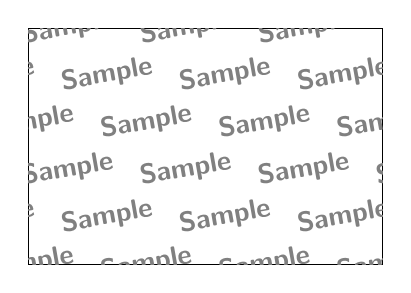
\begin{tikzpicture}
    \draw rectangle++(4.5,3);
    \clip rectangle++(4.5,3);
    \foreach\x in{0,1,2,3,4}{
      \foreach\y in{0,1,2,3,4,5,6}{
        \path(\x*1.5-\y*0.5,\y*0.6)node[rotate=10,text=gray]{\sffamily\bfseries\itshape Sample };
      }
    }
  \end{tikzpicture}
  %% 入れる画像：display.launch.py を起動し、RViz2 に RobotModel と TF を表示した画面と、joint_state_publisher_gui のウィンドウのスクリーンショット
  % eps 画像を貼る場合は includegraphics をお使いください。
  % 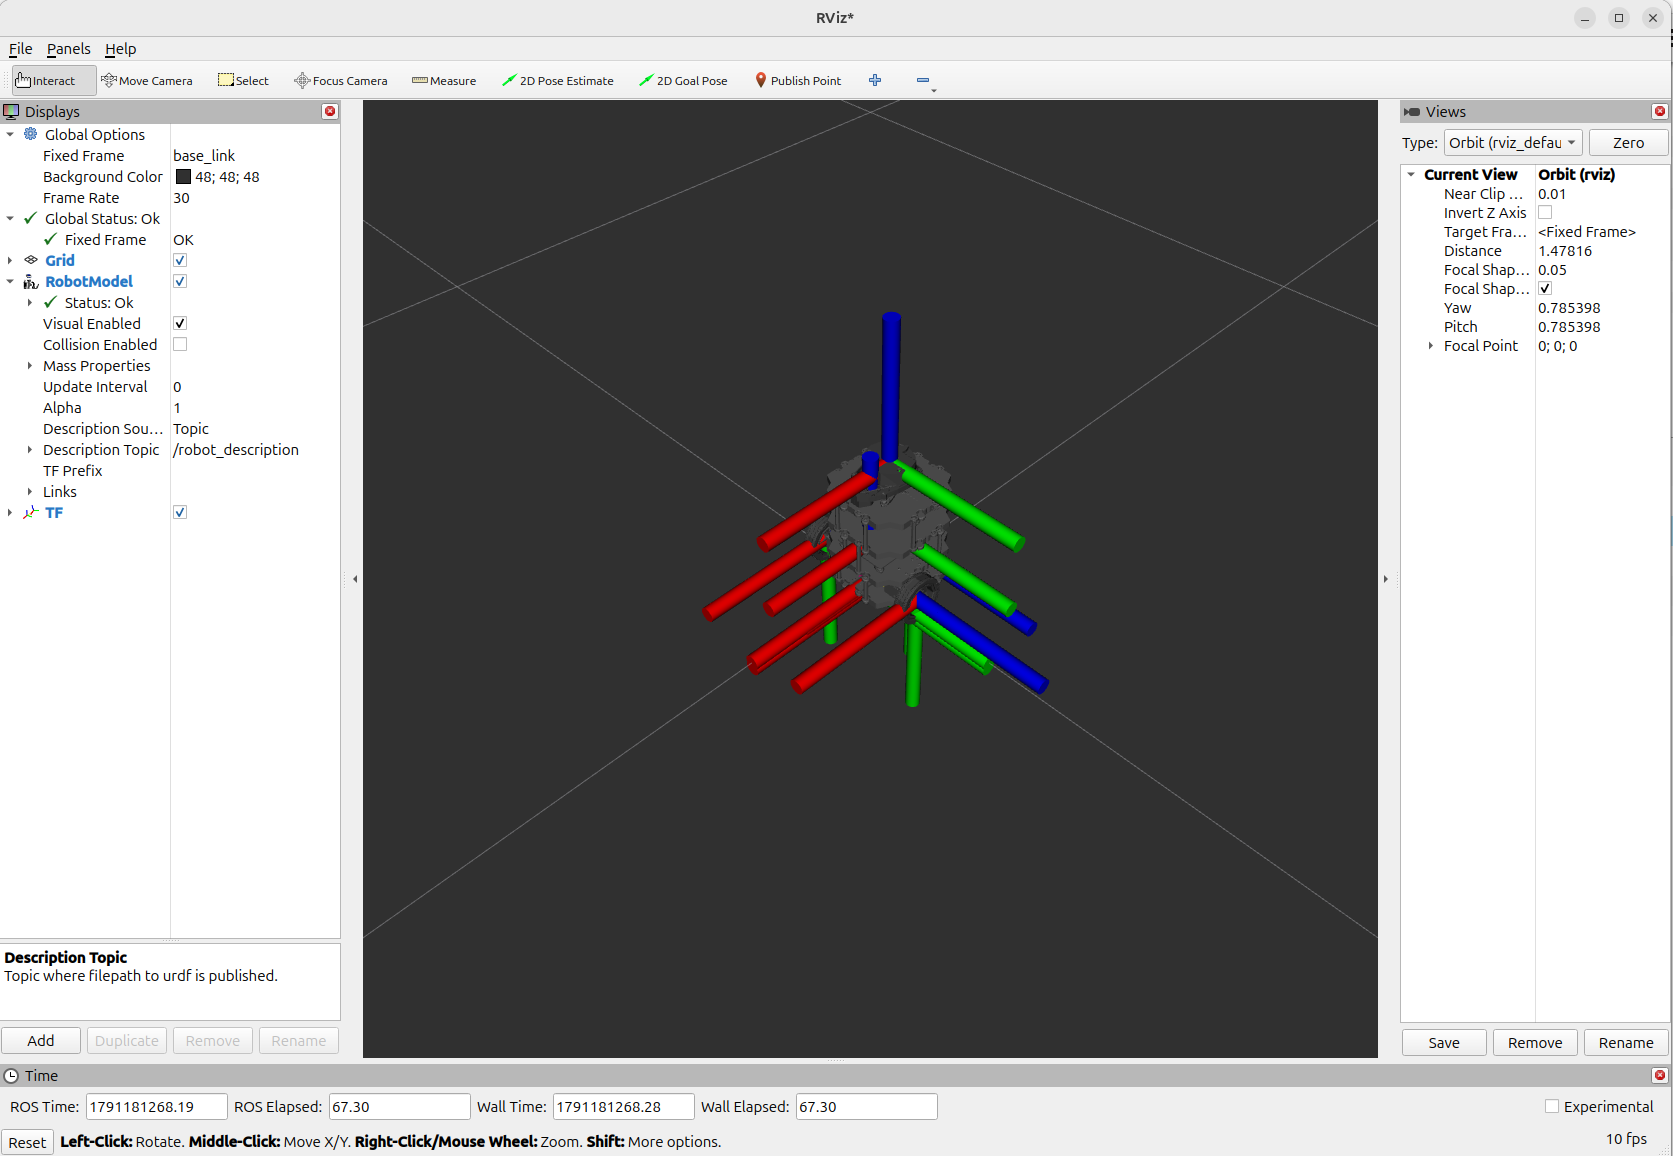
\includegraphics[width=0.8\linewidth]{tf_viz/rviz.png}
  \caption{RViz2 でロボットのモデルと座標系を表示した例}
  \label{fig:tf-viz-rviz}
\end{figure}

RViz2 でよく使う表示（Display）には、次のようなものがあります。
「Add」の画面の「By topic」タブを使うと、今流れているトピックの中から選んで追加することもできます。

\begin{tablebox}[RViz2 のよく使う表示][tab:tf-viz-displays]
  \begin{tabular}{lp{0.6\linewidth}}
    \toprule
    表示 & 表示するもの \\
    \midrule
    RobotModel & URDF のロボットのモデル \\
    TF & 座標系の位置と向き \\
    LaserScan & LiDAR で測った点（\cmd{sensor\_msgs/msg/LaserScan}） \\
    Image & カメラの画像（\cmd{sensor\_msgs/msg/Image}） \\
    Map & 地図（\ref{sec:practice-slam}節） \\
    Path & 計画した経路 \\
    \bottomrule
  \end{tabular}
\end{tablebox}

\subsection{設定を保存する}

RViz2 を閉じると、設定は消えてしまいます。
メニューの「File」→「Save Config As」で、設定を \cmd{.rviz} という拡張子のファイルに保存しておくと、次からは \cmd{rviz2 -d ファイル名.rviz} で、同じ設定で起動できます。
launch ファイルから起動するときは、\cmd{Node} に \cmd{arguments=['-d', 設定ファイルの場所]} を書きます。

\begin{caution}[VirtualBox で RViz2 が表示されないとき]
  VirtualBox などの仮想マシンでは、3D の表示がうまくいかず、RViz2 の画面が真っ黒になったり、起動してすぐに終了したりすることがあります。
  そのときは、次のように、3D の計算を CPU で行う設定にしてから起動してみましょう。
\begin{lstlisting}[numbers=none, xleftmargin=0pt, framexleftmargin=0pt]
$ export LIBGL_ALWAYS_SOFTWARE=1
$ rviz2
\end{lstlisting}
  表示は遅くなりますが、動くようになることがあります。
\end{caution}

\section*{この章のまとめ}

\begin{itemize}
  \item ロボットでは、本体・センサ・地図など、たくさんの座標系を使います。ROS 2 では、x 軸が前、y 軸が左、z 軸が上で、単位は m と rad です。
  \item tf2 は、座標系どうしの位置関係を \cmd{/tf} と \cmd{/tf\_static} で管理し、どの 2 つの座標系の間でも座標変換を計算してくれます。\cmd{tf2\_echo} や \cmd{view\_frames} で調べられます。
  \item URDF では、ロボットをリンクとジョイントの組み合わせで書きます。
  \item robot\_state\_publisher は、URDF と \cmd{/joint\_states} から座標変換を計算して、tf2 に流します。
  \item RViz2 で、ロボットのモデル・座標系・センサのデータなどを表示できます。設定は \cmd{.rviz} ファイルに保存しておきましょう。
\end{itemize}

\chapter{シミュレーション}
\label{chap:simulation}

% この章で学ぶこと
\begin{goalbox}
  \begin{itemize}
    \item ロボットのシミュレータ Gazebo の概要と、シミュレーションを使う理由
    \item ros\_gz\_bridge による Gazebo と ROS 2 の連携のしくみ
    \item TurtleBot3 を使って、移動ロボットをシミュレーションの中で動かす方法
    \item LiDAR・カメラ・IMU のシミュレーションと、そのデータの見方
  \end{itemize}
\end{goalbox}

ロボットのプログラムを書いても、実際のロボットがなければ試せない、というのでは困ります。
また、ロボットを持っていても、書いたばかりのプログラムをいきなり動かすと、壁にぶつかって壊れてしまうかもしれません。
そこで、コンピュータの中に仮想の世界とロボットを作り、その中でロボットを動かす\textbf{シミュレーション}を使います。
この章では、ROS 2 とよく組み合わせて使われるシミュレータ Gazebo で、移動ロボットを動かしてみます。

\section{Gazebo の概要}
\label{sec:simulation-gazebo}

\subsection{シミュレーションを使う理由}

シミュレーションには、次のような利点があります。

\begin{itemize}
  \item ロボットがなくても、プログラムを試せる
  \item ぶつかっても壊れないので、失敗を恐れずに何度でも試せる
  \item 同じ条件で、何度でも繰り返して試せる
  \item 広い建物や屋外など、用意するのが難しい環境でも試せる
\end{itemize}

ただし、シミュレーションの世界は、現実の世界を単純にしたものです。
床のすべりやすさ、センサの雑音、光の当たり方などは、現実と完全には同じになりません。
シミュレーションでうまく動いたプログラムでも、実際のロボットでは調整が必要になることが多い、ということを覚えておきましょう。

\subsection{Gazebo}

\textbf{Gazebo} は、ロボットのためのオープンソースのシミュレータです。
重力や摩擦、物体どうしの衝突などの物理法則を計算して、ロボットの動きを再現します。
また、LiDAR やカメラ、IMU（加速度と角速度を測るセンサ）などのセンサも再現でき、センサが測るはずのデータを作ってくれます。

Gazebo には、古い「Gazebo Classic」（Gazebo 11 まで）と、作り直された新しい「Gazebo」（以前は Ignition Gazebo と呼ばれていました）があります。
Gazebo Classic は 2025 年にサポートが終了しており、ROS 2 Jazzy では、新しい Gazebo の \textbf{Harmonic} というバージョンを使います。
インターネットで調べるときは、\cmd{gazebo} コマンドや \cmd{gazebo\_ros} パッケージを使っている記事は Gazebo Classic のものなので、注意しましょう。

\begin{tablebox}[ROS 2 と Gazebo の組み合わせ][tab:simulation-versions]
  \begin{tabular}{lll}
    \toprule
    ROS 2 & Gazebo & ROS 2 と連携するパッケージ \\
    \midrule
    Humble & Gazebo Classic または Fortress & \cmd{gazebo\_ros} または \cmd{ros\_gz} \\
    Jazzy（本書） & Harmonic & \cmd{ros\_gz} \\
    \bottomrule
  \end{tabular}
\end{tablebox}

\subsection{Gazebo をインストールして起動する}

ROS 2 Jazzy と組み合わせて使う Gazebo は、\cmd{ros-jazzy-ros-gz} パッケージをインストールすると、一緒にインストールされます。

\begin{terminal}[Gazebo をインストールする]
$ sudo apt install ros-jazzy-ros-gz
\end{terminal}

Gazebo は、\cmd{gz sim} コマンドで起動します。
後ろには、シミュレーションする世界を書いた \textbf{SDF} ファイル（XML の形式）を指定します。
Gazebo に付属している、いくつかの形の物体が置かれた世界を開いてみましょう。

\begin{terminal}[Gazebo を起動する]
$ gz sim shapes.sdf
\end{terminal}

左下の再生ボタン（▶）を押すと、シミュレーションの時間が進み始めます。
マウスの左ドラッグで視点を動かし、右ドラッグで拡大・縮小、ホイールを押しながらドラッグで回転できます。

\begin{caution}[仮想マシンでの Gazebo]
  Gazebo は、3D の表示と物理の計算に、多くの計算量を使います。
  VirtualBox などの仮想マシンでは、動きがとても遅くなったり、画面が正しく表示されなかったりすることがあります。
  VirtualBox の設定で、仮想マシンに割り当てる CPU のコア数とメモリを増やし、ディスプレイの「3D アクセラレーションを有効化」を試してみましょう（\ref{sec:linux-setup}節）。
  それでも動かないときは、RViz2 と同じく \cmd{export LIBGL\_ALWAYS\_SOFTWARE=1} を試すか（\ref{sec:tf-viz-rviz}節）、Ubuntu を直接インストールしたパソコンを使うことを検討してください。
\end{caution}

\section{Gazebo と ROS 2 の連携}
\label{sec:simulation-bridge}

\subsection{ros\_gz\_bridge}

Gazebo は、ROS 2 とは別のソフトウェアで、内部では独自の通信のしくみ（Gazebo Transport）を使っています。
そのため、ROS 2 のノードから Gazebo の中のロボットを動かしたり、センサのデータを受け取ったりするには、両者の間でメッセージを変換して中継する必要があります。
この役目をするのが、\textbf{ros\_gz\_bridge} です（図\ref{fig:simulation-bridge}）。

\begin{figure}[tb]
  \centering
  % 図：Gazebo と ROS 2 のつながり（chapters/ros2/simulation.tex）
\begin{tikzpicture}[blk/.style={draw, rounded corners=3pt, align=center, font=\small, minimum height=10mm, inner sep=4pt},
    msg/.style={font=\scriptsize\ttfamily, midway, fill=white, inner sep=1pt}]
  \node[blk, fill=orange!10, minimum width=34mm, minimum height=34mm] (gz) at (0,0) {};
  \node[font=\small\bfseries, anchor=north] at (gz.north) {Gazebo};
  \node[blk, fill=white, font=\scriptsize, minimum width=28mm] at (0,0.15) {ロボットのモデル\\（車輪・LiDAR・\\カメラ・IMU）};
  \node[font=\scriptsize, anchor=south] at (gz.south) {物理法則で動きを計算};
  \node[blk, fill=green!10, minimum width=24mm, minimum height=34mm] (br) at (4.4,0) {ros\_gz\_bridge\\[2pt]{\scriptsize メッセージを}\\{\scriptsize 変換して中継}};
  \node[blk, fill=blue!8, minimum width=30mm, minimum height=34mm] (ros) at (9.6,0) {};
  \node[font=\small\bfseries, anchor=north] at (ros.north) {ROS 2 のノード};
  \node[font=\scriptsize, align=center] at (9.6,-0.1) {teleop\\自作のノード\\SLAM、Nav2\\RViz2};
  \draw[figarrow] ([yshift=11mm]br.east) -- node[msg, above=1pt]{/scan, /odom} ([yshift=11mm]ros.west);
  \draw[figarrow] ([yshift=4mm]br.east) -- node[msg, above=1pt]{/imu, /clock} ([yshift=4mm]ros.west);
  \draw[figarrow] ([yshift=-11mm]ros.west) -- node[msg, below=1pt]{/cmd\_vel} ([yshift=-11mm]br.east);
  \draw[figarrow] ([yshift=8mm]gz.east) -- node[font=\scriptsize, above=1pt, midway]{センサ} ([yshift=8mm]br.west);
  \draw[figarrow] ([yshift=-11mm]br.west) -- node[font=\scriptsize, below=1pt, midway]{速度の指令} ([yshift=-11mm]gz.east);
\end{tikzpicture}

  \caption{Gazebo と ROS 2 のつながり}
  \label{fig:simulation-bridge}
\end{figure}

ros\_gz\_bridge は、ROS 2 のノードの側から見ると、「Gazebo の中のセンサのデータをパブリッシュし、速度の指令をサブスクライブするノード」に見えます。
そのため、シミュレーションでも、実際のロボットでも、同じトピック名と型でやり取りするようにしておけば、自分のノードは書き換えずにそのまま使えます。

\subsection{ブリッジの設定}

ros\_gz\_bridge には、「どの Gazebo のトピックを、どの ROS 2 のトピックに、どちら向きに中継するか」を設定します。
コマンドで 1 つずつ指定することもできますが、たくさんのトピックを中継するときは、YAML ファイルに書くのが一般的です。
次は、LiDAR のデータと速度の指令を中継する設定の例です。

\begin{codelisting}{ros\_gz\_bridge の設定の例}{lst:simulation-bridge-yaml}
- ros_topic_name: "scan"
  gz_topic_name: "scan"
  ros_type_name: "sensor_msgs/msg/LaserScan"
  gz_type_name: "gz.msgs.LaserScan"
  direction: GZ_TO_ROS        # Gazebo から ROS 2 へ

- ros_topic_name: "cmd_vel"
  gz_topic_name: "cmd_vel"
  ros_type_name: "geometry_msgs/msg/TwistStamped"
  gz_type_name: "gz.msgs.Twist"
  direction: ROS_TO_GZ        # ROS 2 から Gazebo へ
\end{codelisting}

この章で使う TurtleBot3 のシミュレーションのパッケージには、このような設定がすでに用意されていて、launch ファイルで ros\_gz\_bridge も一緒に起動されます。
自分でロボットのモデルを作るときに、このような設定を書くことになります。

\subsection{シミュレーションの時刻}

シミュレーションでは、コンピュータが遅いと、シミュレーションの中の時間が、現実の時間よりゆっくり進むことがあります。
また、シミュレーションを一時停止すると、シミュレーションの中の時間も止まります。
そのため、ROS 2 のノードは、パソコンの時計ではなく、シミュレーションの時計を使う必要があります。

シミュレーションの時刻は、\cmd{/clock} トピックにパブリッシュされます。
各ノードの \cmd{use\_sim\_time} パラメータを \cmd{true} にすると、そのノードは \cmd{/clock} の時刻を使うようになります。
シミュレーションと組み合わせてノードを起動するときは、\cmd{use\_sim\_time} を \cmd{true} にするのを忘れないようにしましょう。

\begin{terminal}[シミュレーションの時刻を使ってノードを起動する]
$ ros2 run my_package param_node --ros-args -p use_sim_time:=true
\end{terminal}

launch ファイルの YAML でまとめて設定するときは、\ref{sec:launch-yaml}節の \cmd{/**} を使うと便利です。

\section{移動ロボットをシミュレーションで動かす}
\label{sec:simulation-turtlebot3}

\subsection{TurtleBot3}

\textbf{TurtleBot3} は、ROBOTIS 社が開発した、ROS の学習や研究のための小型の移動ロボットです。
左右 2 つの車輪で動き、LiDAR を搭載しています。
世界中で使われていて、シミュレーションのモデルや、地図作り・自律移動のサンプルも公開されているので、ROS 2 を学ぶ題材として最適です。
TurtleBot3 には、小さな「Burger」と、少し大きくカメラも搭載できる「Waffle」などのモデルがあります。

\subsection{TurtleBot3 のシミュレーションを用意する}

TurtleBot3 の本体のパッケージは apt でインストールし、シミュレーションのパッケージは、\ref{sec:workspace-colcon}節と同じように、ソースコードからワークスペースでビルドします。

\begin{terminal}[TurtleBot3 のパッケージをインストールする]
$ sudo apt install ros-jazzy-turtlebot3 ros-jazzy-turtlebot3-msgs
$ cd ~/ros2_ws/src
~/ros2_ws/src$ git clone -b jazzy https://github.com/ROBOTIS-GIT/turtlebot3_simulations.git
~/ros2_ws/src$ cd ~/ros2_ws
~/ros2_ws$ rosdep install -i --from-path src --rosdistro jazzy -y
~/ros2_ws$ colcon build --symlink-install
~/ros2_ws$ source install/local_setup.bash
\end{terminal}

TurtleBot3 のパッケージは、環境変数 \cmd{TURTLEBOT3\_MODEL}（\ref{chap:env}章）で、どのモデルを使うかを決めます。
毎回設定しなくて済むように、\cmd{.bashrc} に書いておきましょう（\ref{sec:env-bashrc}節）。

\begin{terminal}[使うモデルを .bashrc に設定する]
~/ros2_ws$ echo 'export TURTLEBOT3_MODEL=burger' >> ~/.bashrc
~/ros2_ws$ source ~/.bashrc
\end{terminal}

\subsection{シミュレーションを起動する}

TurtleBot3 と、障害物が置かれた世界を、Gazebo で起動します。

\begin{terminal}[TurtleBot3 のシミュレーションを起動する]
~/ros2_ws$ ros2 launch turtlebot3_gazebo turtlebot3_world.launch.py
\end{terminal}

Gazebo の画面に、六角形の壁の中に柱が並んだ世界と、そこに置かれた TurtleBot3 が表示されます（図\ref{fig:simulation-tb3}）。
初めて起動するときは、モデルのダウンロードなどで、表示されるまでに時間がかかることがあります。

\begin{figure}[tb]
  \centering
  \large
  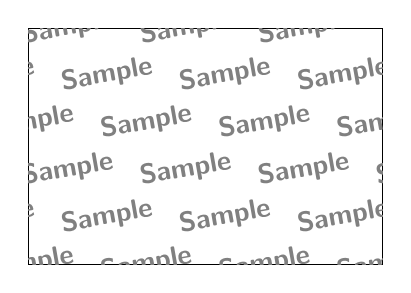
\begin{tikzpicture}
    \draw rectangle++(4.5,3);
    \clip rectangle++(4.5,3);
    \foreach\x in{0,1,2,3,4}{
      \foreach\y in{0,1,2,3,4,5,6}{
        \path(\x*1.5-\y*0.5,\y*0.6)node[rotate=10,text=gray]{\sffamily\bfseries\itshape Sample };
      }
    }
  \end{tikzpicture}
  %% 入れる画像：turtlebot3_world.launch.py を起動したときの Gazebo の画面（六角形の壁の中に柱が並んだ世界と TurtleBot3 Burger）のスクリーンショット
  % eps 画像を貼る場合は includegraphics をお使いください。
  % 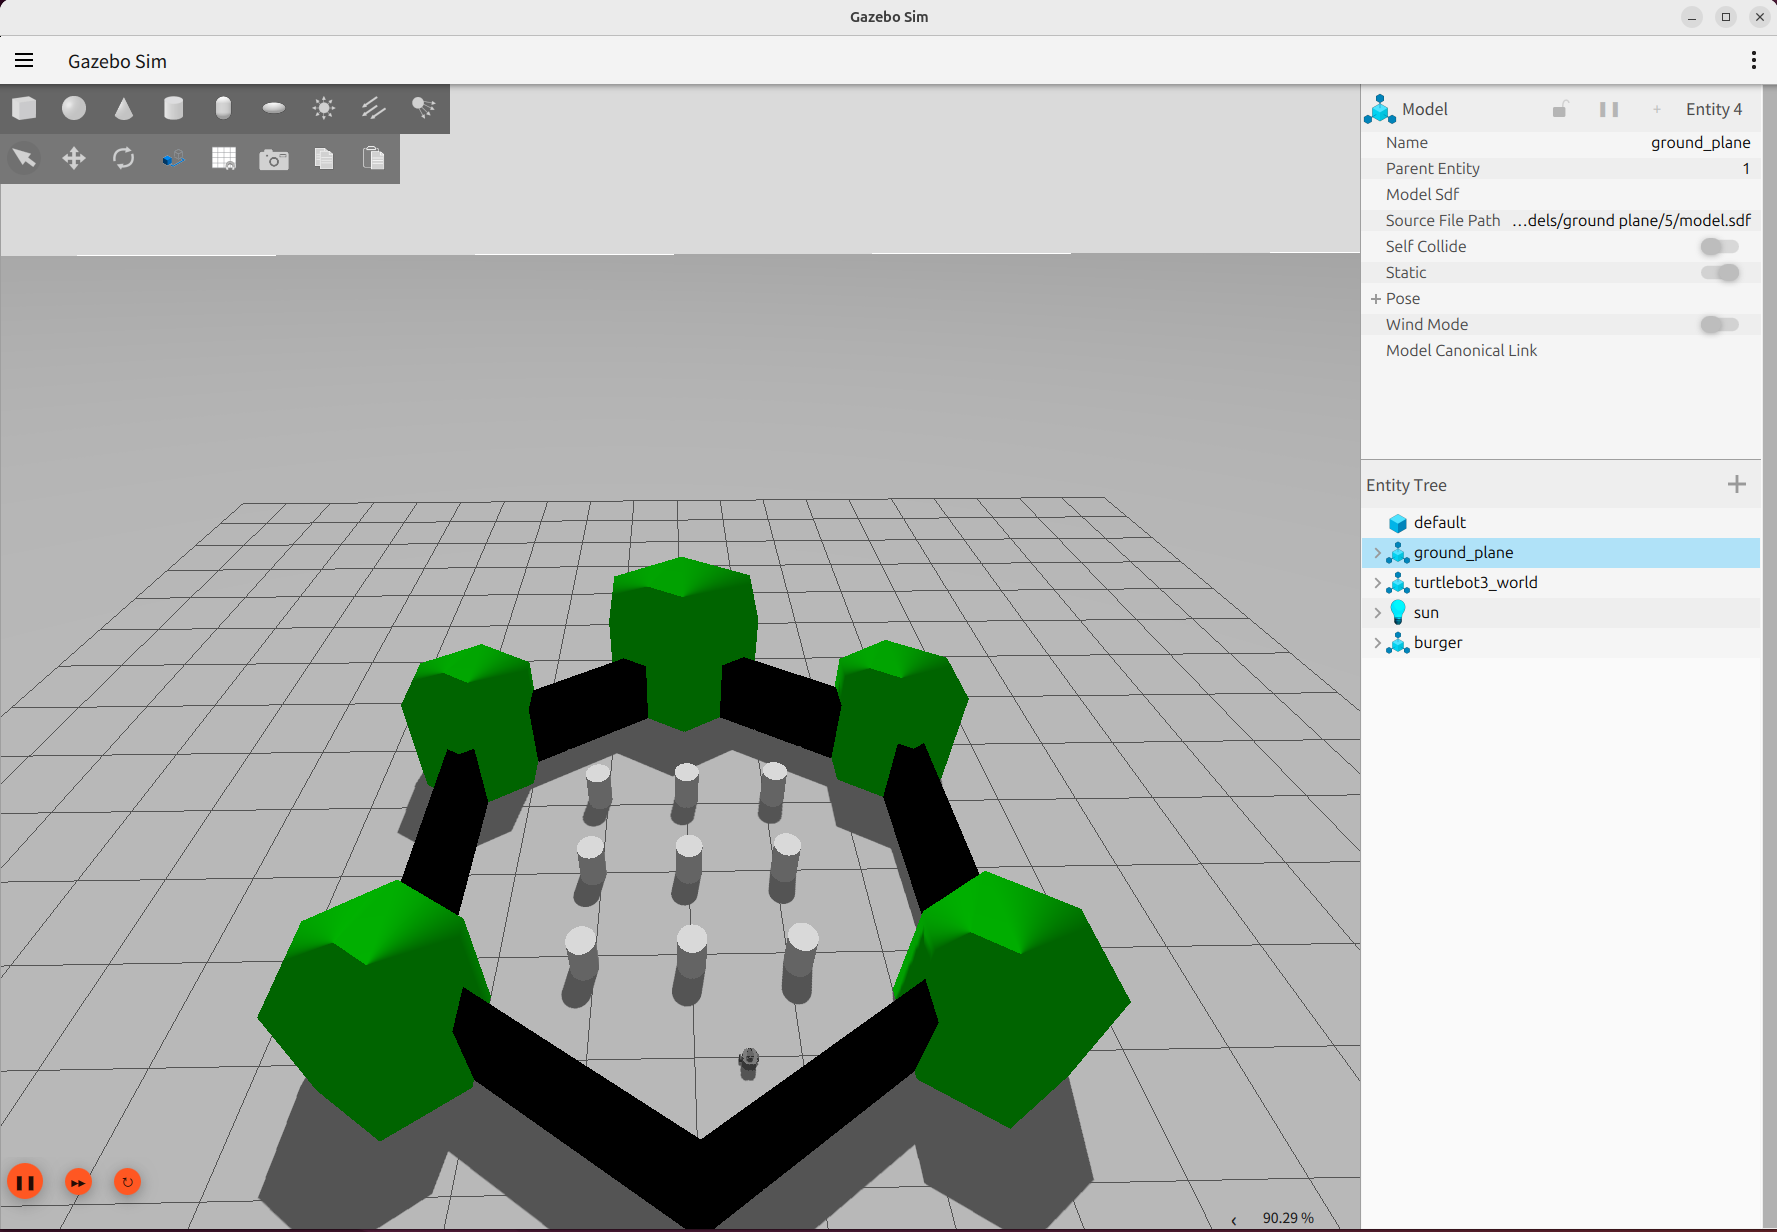
\includegraphics[width=0.8\linewidth]{simulation/turtlebot3_world.png}
  \caption{Gazebo で TurtleBot3 を起動した様子}
  \label{fig:simulation-tb3}
\end{figure}

別のターミナルで、トピックの一覧を見てみましょう。

\begin{terminal}[シミュレーションのトピックの一覧]
~/ros2_ws$ ros2 topic list
/clock
/cmd_vel
/imu
/joint_states
/odom
/robot_description
/scan
/tf
/tf_static
...
\end{terminal}

\cmd{/scan}（LiDAR）、\cmd{/odom}（オドメトリ）、\cmd{/imu}（IMU）、\cmd{/cmd\_vel}（速度の指令）、\cmd{/tf} などのトピックが、ros\_gz\_bridge や robot\_state\_publisher（\ref{sec:tf-viz-rsp}節）によってパブリッシュされていることがわかります。
シミュレーションの中のロボットも、ROS 2 から見れば、これらのトピックを持ったノードの集まりなのです。

\subsection{キーボードで動かす}

TurtleBot3 には、キーボードで操作するためのノードが用意されています。

\begin{terminal}[TurtleBot3 をキーボードで操作する]
~/ros2_ws$ ros2 run turtlebot3_teleop teleop_keyboard
...
Moving around:
        w
   a    s    d
        x

w/x : increase/decrease linear velocity (Burger : ~ 0.22)
a/d : increase/decrease angular velocity (Burger : ~ 2.84)

space key, s : force stop
\end{terminal}

このターミナルを選んだ状態で \key{W} を押すと前進の速度が上がり、\key{X} で下がります。
\key{A} と \key{D} で回転の速度が変わり、\key{S} か \key{Space} で止まります。
ロボットを動かしながら、\cmd{ros2 topic echo /odom} でオドメトリが変わっていく様子も確かめてみましょう。

\begin{point}[TwistStamped]
  ROS 2 Jazzy の TurtleBot3 は、速度の指令に、\cmd{Twist}（\ref{sec:ros2-concepts-topic}節）ではなく \cmd{geometry\_msgs/msg/TwistStamped} 型を使います。
  \cmd{TwistStamped} は、\cmd{Twist} に、時刻と座標系の名前が入った \cmd{header} を加えたメッセージ型です。
\begin{lstlisting}[numbers=none, xleftmargin=0pt, framexleftmargin=0pt]
std_msgs/Header header      # 時刻（stamp）と座標系の名前（frame_id）
Twist twist                 # 今までの Twist と同じ
\end{lstlisting}
  \cmd{ros2 topic info /cmd\_vel} で、トピックの型を確かめる習慣をつけておきましょう。
\end{point}

\section{センサのシミュレーション}
\label{sec:simulation-sensor}

\subsection{LiDAR}

TurtleBot3 Burger には、周りの物までの距離を、ぐるりと 360 度測る LiDAR が搭載されています。
LiDAR のデータは、\cmd{/scan} トピックに \cmd{sensor\_msgs/msg/LaserScan} 型でパブリッシュされます。
型の中身の主な部分を見てみましょう。

\begin{terminal}[LaserScan 型の中身（一部）]
~/ros2_ws$ ros2 interface show sensor_msgs/msg/LaserScan
std_msgs/Header header
float32 angle_min        # start angle of the scan [rad]
float32 angle_max        # end angle of the scan [rad]
float32 angle_increment  # angular distance between measurements [rad]
...
float32 range_min        # minimum range value [m]
float32 range_max        # maximum range value [m]
float32[] ranges         # range data [m]
...
\end{terminal}

\cmd{ranges} は、測った距離のリストです。
1 つ目の値は \cmd{angle\_min} の向き、2 つ目の値はそこから \cmd{angle\_increment} だけ回った向き……というように、向きを少しずつ変えながら測った距離が並んでいます。
\cmd{range\_min} より近い値や、\cmd{range\_max} より遠い値（何も当たらなかったときは \cmd{inf}）は、正しく測れなかった値として扱います。
\ref{sec:practice-avoid}節では、このデータを読んで障害物を避けるノードを作ります。

\cmd{--once} を付けると、1 回分のメッセージだけを表示できます。
\cmd{ranges} は長いので、\cmd{--field} で見たい部分だけを表示するとよいでしょう。

\begin{terminal}[LaserScan の一部だけを表示する]
~/ros2_ws$ ros2 topic echo --once --field range_max /scan
3.5
---
\end{terminal}

\subsection{RViz2 でセンサのデータを見る}

センサのデータは、数値で見るより、RViz2（\ref{sec:tf-viz-rviz}節）で表示したほうがわかりやすくなります。
\cmd{use\_sim\_time} を \cmd{true} にして RViz2 を起動し、次のように設定してみましょう。

\begin{terminal}[シミュレーションの時刻を使って RViz2 を起動する]
~/ros2_ws$ rviz2 --ros-args -p use_sim_time:=true
\end{terminal}

\begin{enumerate}
  \item 「Fixed Frame」を \cmd{odom} にします。
  \item 「Add」から「RobotModel」を追加し、「Description Topic」を \cmd{/robot\_description} にします。
  \item 「Add」の「By topic」タブから、\cmd{/scan} の「LaserScan」を追加します。
\end{enumerate}

ロボットの周りに、LiDAR が測った点が表示され、柱の形が浮かび上がります。
キーボードでロボットを動かすと、点の見え方が変わっていく様子がわかります。

\subsection{カメラと IMU}

TurtleBot3 Waffle には、カメラも搭載されています。
\cmd{TURTLEBOT3\_MODEL} を \cmd{waffle} にしてシミュレーションを起動すると、カメラの画像が \cmd{sensor\_msgs/msg/Image} 型でパブリッシュされます。
画像は、RViz2 の「Image」の表示か、\cmd{rqt\_image\_view} で見られます。

\begin{terminal}[Waffle でシミュレーションを起動して、カメラの画像を見る]
~/ros2_ws$ TURTLEBOT3_MODEL=waffle ros2 launch turtlebot3_gazebo turtlebot3_world.launch.py
$ ros2 run rqt_image_view rqt_image_view   # 別のターミナルで
\end{terminal}

\cmd{rqt\_image\_view} の画面の左上で、画像のトピック（\cmd{/camera/image\_raw} など）を選ぶと、ロボットから見た景色が表示されます。
コマンドの前に \cmd{変数名=値} を書くと、そのコマンドを実行するときだけ環境変数を設定できます（\ref{sec:env-export-source}節）。

IMU のデータは、\cmd{/imu} トピックに \cmd{sensor\_msgs/msg/Imu} 型でパブリッシュされます。
ロボットの向き（クォータニオン）、角速度、加速度が入っていて、ロボットを回転させると \cmd{angular\_velocity.z} の値が変わります。

\begin{terminal}[IMU のデータを表示する]
~/ros2_ws$ ros2 topic echo --field angular_velocity /imu
\end{terminal}

シミュレーションのセンサにも、設定によっては現実のセンサのような雑音が加えられています。
センサの値が少しずつ揺れるのは、そのためです。
現実のセンサには必ず雑音があるので、それでもうまく動くプログラムを書くことが大切です。

\section*{この章のまとめ}

\begin{itemize}
  \item シミュレーションを使うと、ロボットがなくても、壊す心配なく、何度でもプログラムを試せます。ただし、現実と完全には同じになりません。
  \item ROS 2 Jazzy では、新しい Gazebo（Harmonic）を使います。Gazebo Classic の情報と混同しないように注意しましょう。
  \item ros\_gz\_bridge が、Gazebo と ROS 2 の間でメッセージを中継します。シミュレーションと組み合わせるノードは、\cmd{use\_sim\_time} を \cmd{true} にします。
  \item TurtleBot3 のシミュレーションでは、\cmd{/scan}・\cmd{/odom}・\cmd{/imu}・\cmd{/cmd\_vel} などのトピックで、ロボットとやり取りできます。
  \item LiDAR のデータ（\cmd{LaserScan}）は、向きを少しずつ変えながら測った距離のリストです。RViz2 で表示すると、周りの様子がよくわかります。
\end{itemize}

\chapter{データの記録とデバッグ}
\label{chap:debug}

% この章で学ぶこと
\begin{goalbox}
  \begin{itemize}
    \item rosbag2 を使って、トピックのデータを記録・再生する方法
    \item ログのレベルと、ログの出し方・見方
    \item ROS 2 でよくあるトラブルと、その原因の調べ方
    \item QoS の設定と、QoS が合わないときに起きること
  \end{itemize}
\end{goalbox}

ロボットのプログラムは、なかなか思ったとおりには動きません。
しかも、ロボットのプログラムの不具合は、「さっきは壁にぶつかったのに、もう一度試したらぶつからなかった」のように、同じ状況を再現するのが難しいことがよくあります。
この章では、ロボットのデータを記録して後から何度でも再生できる rosbag2 と、ログの使い方、そして ROS 2 でよくあるトラブルの調べ方を学びます。
\ref{sec:python-class-debug}節で学んだ Python のデバッグの基本も、思い出しながら読んでください。

\section{rosbag2 による記録と再生}
\label{sec:debug-rosbag}

\subsection{rosbag2 とは}

\textbf{rosbag2} は、トピックに流れたメッセージを、時刻と一緒にファイルに記録し、後から同じタイミングで再生するためのツールです。
記録したファイルを \textbf{bag ファイル}（バッグファイル）といいます。
bag ファイルを使うと、次のようなことができます。

\begin{itemize}
  \item 実際のロボットで記録したセンサのデータを、ロボットがない場所で再生して、プログラムを試す
  \item 不具合が起きたときのデータを記録しておき、同じ状況を何度でも再現して原因を調べる
  \item 実験のデータを保存しておき、後から解析する
\end{itemize}

\subsection{記録する}

turtlesim を使って、試してみましょう。
\cmd{turtlesim\_node} と \cmd{turtle\_teleop\_key} を起動しておき（\ref{chap:ros2_concepts}章）、別のターミナルで \cmd{ros2 bag record} を実行します。
後ろには、記録するトピックを並べます。
\cmd{-o} で、記録する bag ファイルの名前（ディレクトリ名）を指定できます。

\begin{terminal}[トピックを記録する]
$ mkdir ~/bag_files && cd ~/bag_files
$ ros2 bag record -o turtle_bag /turtle1/cmd_vel /turtle1/pose
[INFO] [...] [rosbag2_recorder]: Press SPACE for pausing/resuming
...
[INFO] [...] [rosbag2_recorder]: Subscribed to topic '/turtle1/cmd_vel'
[INFO] [...] [rosbag2_recorder]: Subscribed to topic '/turtle1/pose'
\end{terminal}

記録している間に、\cmd{turtle\_teleop\_key} でカメを動かします。
動かし終わったら、\cmd{ros2 bag record} のターミナルで \key{Ctrl}+\key{C} を押して、記録を終わります。
すべてのトピックを記録したいときは、トピック名の代わりに \cmd{-a} を付けます。
ただし、カメラの画像などを記録すると、すぐにファイルが大きくなるので注意しましょう。

\subsection{記録した内容を確かめる}

\cmd{ros2 bag info} で、bag ファイルに何が記録されているかを確かめられます。

\begin{terminal}[bag ファイルの情報を表示する]
$ ros2 bag info turtle_bag
Files:             turtle_bag_0.mcap
Bag size:          102.5 KiB
Storage id:        mcap
Duration:          25.4s
Start:             Oct  2 2026 10:00:00.123 (1790902800.123)
End:               Oct  2 2026 10:00:25.523 (1790902825.523)
Messages:          1609
Topic information: Topic: /turtle1/cmd_vel | Type: geometry_msgs/msg/Twist | Count: 21 | Serialization Format: cdr
                   Topic: /turtle1/pose | Type: turtlesim/msg/Pose | Count: 1588 | Serialization Format: cdr
\end{terminal}

記録した時間、トピックごとのメッセージの型と数がわかります。
ROS 2 Jazzy では、bag ファイルは \textbf{MCAP} という形式で保存されます。

\subsection{再生する}

\cmd{ros2 bag play} で、記録したメッセージを再生します。
\cmd{turtle\_teleop\_key} を止め、turtlesim の \cmd{/reset} サービス（\ref{sec:ros2-concepts-service}節）でカメを最初の位置に戻してから、再生してみましょう。

\begin{terminal}[記録したメッセージを再生する]
$ ros2 service call /reset std_srvs/srv/Empty
$ ros2 bag play turtle_bag
\end{terminal}

記録したときと同じように、カメが動きます。
記録された \cmd{/turtle1/cmd\_vel} のメッセージが、記録したときと同じタイミングでパブリッシュされたからです。
ただし、\cmd{/turtle1/pose} も一緒に再生されるので、turtlesim がパブリッシュする \cmd{/turtle1/pose} と混ざってしまいます。
特定のトピックだけを再生したいときは、\cmd{--topics} で指定します。

\begin{tablebox}[ros2 bag play のよく使うオプション][tab:debug-bag-play]
  \begin{tabular}{p{0.38\linewidth}p{0.52\linewidth}}
    \toprule
    オプション & 意味 \\
    \midrule
    \cmd{--topics トピック名 ...} & 指定したトピックだけを再生する \\
    \cmd{--rate 0.5} & 0.5 倍の速さで再生する（2 なら 2 倍） \\
    \cmd{--loop} & 最後まで再生したら、最初から繰り返す \\
    \cmd{--clock} & \cmd{/clock} もパブリッシュする（\cmd{use\_sim\_time} と組み合わせる） \\
    \bottomrule
  \end{tabular}
\end{tablebox}

再生中に \key{Space} を押すと、一時停止と再開ができます。

\begin{point}[bag ファイルで自分のノードを試す]
  実際のロボットやシミュレーションで、\cmd{/scan} や \cmd{/odom} などのセンサのデータを記録しておけば、ロボットを動かさなくても、自分のノードに同じデータを何度でも流して試せます。
  このとき、\cmd{ros2 bag play --clock} で再生し、自分のノードは \cmd{use\_sim\_time} を \cmd{true}（\ref{sec:simulation-bridge}節）にして起動すると、記録したときの時刻で動かせます。
\end{point}

\section{ログ出力とログレベル}
\label{sec:debug-log}

\subsection{ログレベル}

\ref{sec:rclpy-first}節では、\cmd{get\_logger().info()} でログを出力しました。
ログには、重要度に応じて 5 つの\textbf{ログレベル}があります。

\begin{tablebox}[ログレベル][tab:debug-log-levels]
  \begin{tabular}{llp{0.5\linewidth}}
    \toprule
    レベル & Python の書き方 & 使う場面 \\
    \midrule
    DEBUG & \cmd{get\_logger().debug()} & 開発中に、細かい値や処理の流れを確かめるため \\
    INFO & \cmd{get\_logger().info()} & 起動した、接続した、など、普段の動作の報告 \\
    WARN & \cmd{get\_logger().warn()} & 動作は続けられるが、注意が必要なこと \\
    ERROR & \cmd{get\_logger().error()} & 処理に失敗したこと \\
    FATAL & \cmd{get\_logger().fatal()} & 動作を続けられない、重大な問題 \\
    \bottomrule
  \end{tabular}
\end{tablebox}

ノードは、決められたレベル以上のログだけを出力します。
標準では INFO 以上が出力され、DEBUG のログは表示されません。
デバッグのための細かいログは DEBUG で書いておき、必要なときだけ表示するようにすると、普段の出力が見やすくなります。

\subsection{ログレベルを変える}

起動するときに、\cmd{--ros-args --log-level} でログレベルを変えられます。

\begin{terminal}[DEBUG のログも表示する]
$ ros2 run my_package talker --ros-args --log-level debug
\end{terminal}

この方法では、rclpy の内部のログも表示されて、多すぎることがあります。
特定のノードだけ変えたいときは、\cmd{--log-level ノード名:=debug} のように、ノード名を付けて指定します。

\subsection{ログを出しすぎないために}

タイマのコールバックの中で毎回ログを出すと、ログがあふれて読めなくなります。
rclpy では、ログの出し方を制限するための引数が用意されています。

\begin{codelisting}[style=python]{ログの出し方を制限する}{lst:debug-log-throttle}
# 1 秒に 1 回まで出力する
self.get_logger().info(f'距離: {d:.2f} m', throttle_duration_sec=1.0)
# 最初の 1 回だけ出力する
self.get_logger().warn('LiDAR のデータが届いていません', once=True)
\end{codelisting}

\subsection{ログの行き先}

ノードが出力したログは、次の 3 か所に送られます。

\begin{itemize}
  \item ノードを起動したターミナル
  \item \cmd{/rosout} トピック（\ref{chap:ros2_concepts}章で見た、自動で用意されるトピック）
  \item \cmd{\textasciitilde/.ros/log/} の下のログファイル
\end{itemize}

launch ファイルでたくさんのノードを起動していると、ターミナルではどのログがどのノードのものか、わかりにくくなります。
そのようなときは、\textbf{rqt\_console} を使うと、\cmd{/rosout} に届いたすべてのノードのログを一覧で表示し、レベルやノード名で絞り込めます。

\begin{terminal}[rqt\_console でログを見る]
$ ros2 run rqt_console rqt_console
\end{terminal}

\section{よくあるトラブルと対処法}
\label{sec:debug-trouble}

\subsection{まず確かめること}

ROS 2 で思ったとおりに動かないときは、次の順番で確かめていくと、原因を絞り込みやすくなります。

\begin{enumerate}
  \item エラーメッセージを読む。最初に出たエラーから読む（\ref{sec:python-class-debug}節）
  \item \cmd{ros2 node list} で、必要なノードが起動しているかを確かめる
  \item \cmd{ros2 topic list} と \cmd{ros2 topic info -v} で、トピックの名前・型・パブリッシャとサブスクライバの数・QoS を確かめる
  \item \cmd{ros2 topic echo} と \cmd{ros2 topic hz} で、データが実際に流れているかを確かめる
  \item \cmd{rqt\_graph} で、ノードとトピックのつながりを確かめる（\ref{sec:ros2-concepts-rqt}節）
\end{enumerate}

\cmd{ros2 doctor} を使うと、ROS 2 の環境やネットワークの設定に問題がないかを、まとめて調べてくれます。

\begin{terminal}[ROS 2 の環境を調べる]
$ ros2 doctor
...
All 5 checks passed
\end{terminal}

\subsection{よくあるトラブル}

ROS 2 でよくあるトラブルと、その主な原因をまとめておきます。
付録\ref{app:troubleshooting}のトラブルシューティング集もあわせて見てください。

\begin{description}
  \item[\cmd{ros2: command not found} と表示される] ROS 2 の設定を読み込んでいません。\cmd{source /opt/ros/jazzy/setup.bash} を実行するか、\cmd{.bashrc} に書かれているかを確かめます（\ref{sec:ros2-install-setup}節）。
  \item[\cmd{Package '〇〇' not found} と表示される] ワークスペースをビルドしていないか、ビルドした後に \cmd{source install/local\_setup.bash} を忘れています（\ref{sec:workspace-overlay}節）。apt でインストールするパッケージなら、インストールされているかを確かめます。
  \item[\cmd{No executable found} と表示される] \cmd{setup.py} の \cmd{entry\_points} にノードを登録していないか、登録した後にビルドし直していません（\ref{sec:rclpy-first}節）。
  \item[Python のファイルを書き換えたのに動作が変わらない] \cmd{--symlink-install} を付けずにビルドしています。ビルドし直しましょう（\ref{sec:workspace-colcon}節）。
  \item[別のパソコンのノードが見えない] 2 台の \cmd{ROS\_DOMAIN\_ID} と \cmd{ROS\_AUTOMATIC\_DISCOVERY\_RANGE} が同じか、同じネットワークにつながっているか、ファイアウォールで通信が止められていないかを確かめます（\ref{sec:ros2-install-network}節）。
  \item[トピックがあるのにデータが届かない] トピックの名前（名前空間やリマップ、\ref{sec:launch-namespace}節）・型・QoS が、パブリッシャとサブスクライバで合っているかを確かめます。QoS については次の節で説明します。
  \item[ノードを止めたのに、一覧に残っている] \cmd{ros2} コマンドは、ノードの情報を覚えておくための\textbf{デーモン}というプロセスを裏で動かしています。古い情報が残っているときは、\cmd{ros2 daemon stop} を実行してから、もう一度調べてみましょう。
  \item[シミュレーションで座標変換や時刻のエラーが出る] ノードによって \cmd{use\_sim\_time} の設定が違っていると、時刻が合わず、\cmd{extrapolation} などのエラーが出ます。すべてのノードで \cmd{use\_sim\_time} をそろえましょう（\ref{sec:simulation-bridge}節）。
\end{description}

\section{QoS 設定の基礎}
\label{sec:debug-qos}

\subsection{QoS とは}

\ref{sec:rclpy-pubsub}節では、パブリッシャとサブスクライバを作るときに、QoS として \cmd{10} を指定しました。
\textbf{QoS}（Quality of Service）は、トピックの通信の品質を決める設定です。
ネットワークが不安定な無線の環境や、大量のデータを送るセンサなど、場面に合わせて通信の仕方を選べるようになっています。
主な設定は、次の 3 つです。

\begin{tablebox}[QoS の主な設定][tab:debug-qos]
  \begin{tabular}{lp{0.28\linewidth}p{0.42\linewidth}}
    \toprule
    設定 & 選べる値 & 意味 \\
    \midrule
    信頼性（Reliability） & \cmd{RELIABLE} & 届かなかったメッセージを送り直して、確実に届ける \\
     & \cmd{BEST\_EFFORT} & 送り直さない。届かなくてもよいので、新しいデータを早く送る \\
    \midrule
    永続性（Durability） & \cmd{VOLATILE} & 後から起動したサブスクライバには、過去のメッセージを送らない \\
     & \cmd{TRANSIENT\_LOCAL} & 後から起動したサブスクライバにも、最後のメッセージを送る \\
    \midrule
    履歴（History） & \cmd{KEEP\_LAST} と数 & 最新の決まった数のメッセージだけを溜めておく \\
     & \cmd{KEEP\_ALL} & すべてのメッセージを溜めておく \\
    \bottomrule
  \end{tabular}
\end{tablebox}

QoS に数字だけを指定すると、\cmd{RELIABLE}・\cmd{VOLATILE}・\cmd{KEEP\_LAST}（その数）になります。

\subsection{場面に合わせた QoS}

たとえば、LiDAR のように 1 秒に何十回も新しいデータを送るセンサでは、途中のデータが 1 つ届かなくても、すぐに次のデータが来ます。
古いデータを送り直すより、新しいデータを早く届けたほうがよいので、\cmd{BEST\_EFFORT} がよく使われます。
一方、地図（\cmd{/map}）は、1 回だけパブリッシュされることが多いので、\cmd{TRANSIENT\_LOCAL} にして、後から起動したノードにも届くようにします。

rclpy には、センサのデータ用の QoS の設定が、\cmd{qos\_profile\_sensor\_data} として用意されています。
QoS を細かく決めるときは、\cmd{QoSProfile} を使います。

\begin{codelisting}[style=python]{QoS を指定してサブスクライバを作る}{lst:debug-qos}
from rclpy.qos import (QoSProfile, ReliabilityPolicy, DurabilityPolicy,
                       qos_profile_sensor_data)

# センサのデータ用の QoS（BEST_EFFORT）
self.create_subscription(LaserScan, 'scan', self.scan_callback,
                         qos_profile_sensor_data)

# 地図のように、後から起動しても最後のメッセージを受け取りたい場合
map_qos = QoSProfile(depth=1,
                     reliability=ReliabilityPolicy.RELIABLE,
                     durability=DurabilityPolicy.TRANSIENT_LOCAL)
self.create_subscription(OccupancyGrid, 'map', self.map_callback, map_qos)
\end{codelisting}

\subsection{QoS が合わないとき}

パブリッシャとサブスクライバの QoS の組み合わせによっては、通信できないことがあります。
特に気をつけたいのは、信頼性の組み合わせです。

\begin{tablebox}[信頼性の組み合わせと通信できるか][tab:debug-qos-compat]
  \begin{tabular}{llc}
    \toprule
    パブリッシャ & サブスクライバ & 通信できるか \\
    \midrule
    \cmd{RELIABLE} & \cmd{RELIABLE} & できる \\
    \cmd{RELIABLE} & \cmd{BEST\_EFFORT} & できる \\
    \cmd{BEST\_EFFORT} & \cmd{BEST\_EFFORT} & できる \\
    \cmd{BEST\_EFFORT} & \cmd{RELIABLE} & \textbf{できない} \\
    \bottomrule
  \end{tabular}
\end{tablebox}

\cmd{BEST\_EFFORT} でパブリッシュしているセンサのデータを、QoS に \cmd{10}（\cmd{RELIABLE}）を指定したサブスクライバで受け取ろうとすると、トピックはあるのにデータが届きません。
このようなときは、\cmd{ros2 topic info -v} で、両者の QoS を確かめましょう。

\begin{terminal}[トピックの QoS を確かめる]
$ ros2 topic info -v /scan
Type: sensor_msgs/msg/LaserScan

Publisher count: 1

Node name: ros_gz_bridge
...
QoS profile:
  Reliability: BEST_EFFORT
  History (Depth): KEEP_LAST (5)
  Durability: VOLATILE
...
\end{terminal}

\cmd{ros2 topic echo} でも、QoS が合わずにデータが表示されないことがあります。
そのときは、\cmd{--qos-reliability best\_effort} のように、QoS を指定して実行します。

\begin{terminal}[QoS を指定してトピックを表示する]
$ ros2 topic echo --qos-reliability best_effort /scan
\end{terminal}

\section*{この章のまとめ}

\begin{itemize}
  \item rosbag2 で、トピックのデータを記録（\cmd{ros2 bag record}）し、後から何度でも再生（\cmd{ros2 bag play}）できます。不具合の再現や、ロボットがない場所での開発に便利です。
  \item ログには DEBUG・INFO・WARN・ERROR・FATAL の 5 つのレベルがあります。\cmd{--log-level} で表示するレベルを変え、rqt\_console でまとめて見られます。
  \item うまく動かないときは、エラーメッセージを読み、ノード・トピック・データの流れを、\cmd{ros2} コマンドで順に確かめていきます。
  \item QoS は通信の品質の設定です。センサのデータは \cmd{BEST\_EFFORT} がよく使われます。QoS が合わないと、トピックがあってもデータが届きません。
\end{itemize}

\chapter{実践：移動ロボットを動かす}
\label{chap:practice}

% この章で学ぶこと
\begin{goalbox}
  \begin{itemize}
    \item キーボードで移動ロボットを操作する方法
    \item LiDAR のデータを読んで、障害物を避けながら走るノードの作り方
    \item SLAM を使って、ロボットに地図を作らせる方法
    \item Navigation2 を使って、地図の上の目的地までロボットを自律移動させる方法
    \item この本の先に進むための道しるべ
  \end{itemize}
\end{goalbox}

この章では、ここまでに学んだことを総動員して、\ref{chap:simulation}章の TurtleBot3 のシミュレーションで、移動ロボットを動かしていきます。
キーボードでの操作から始めて、自分で書いたノードで障害物を避けさせ、最後は、ロボットに地図を作らせて、その地図の上で目的地まで自動で移動させます。
シミュレーションで動くようになれば、同じしくみで、実際のロボットも動かせます（\ref{chap:kachaka}章）。

この章では、すべてのノードをシミュレーションと組み合わせて使うので、自分で起動するノードには \cmd{use\_sim\_time:=true} を付けます（\ref{sec:simulation-bridge}節）。
まず、TurtleBot3 のシミュレーションを起動しておきましょう。

\begin{terminal}[TurtleBot3 のシミュレーションを起動する]
$ ros2 launch turtlebot3_gazebo turtlebot3_world.launch.py
\end{terminal}

\section{キーボードでロボットを操作する}
\label{sec:practice-teleop}

\subsection{teleop\_twist\_keyboard}

\ref{sec:simulation-turtlebot3}節では、TurtleBot3 専用の \cmd{teleop\_keyboard} でロボットを動かしました。
ROS 2 には、TurtleBot3 に限らず、どの移動ロボットでも使える \textbf{teleop\_twist\_keyboard} というノードもあります。
\cmd{/cmd\_vel} トピックに速度の指令をパブリッシュするだけなので、\cmd{/cmd\_vel} で動くロボットなら、シミュレーションでも実際のロボットでも、そのまま使えます。

\begin{terminal}[teleop\_twist\_keyboard をインストールして起動する]
$ sudo apt install ros-jazzy-teleop-twist-keyboard
$ ros2 run teleop_twist_keyboard teleop_twist_keyboard --ros-args -p stamped:=true
...
Moving around:
   u    i    o
   j    k    l
   m    ,    .
...
q/z : increase/decrease max speeds by 10%
\end{terminal}

\cmd{stamped:=true} は、\cmd{Twist} ではなく \cmd{TwistStamped}（\ref{sec:simulation-turtlebot3}節）でパブリッシュするための設定です。
ROS 2 Jazzy の TurtleBot3 は \cmd{TwistStamped} を使うので、この設定が必要です。

\key{I} で前進、\key{,} で後退、\key{J} と \key{L} でその場で回転、\key{K} で停止です。
\key{U}・\key{O}・\key{M}・\key{.} では、曲がりながら進みます。
ほかのキーを押すと停止するので、ロボットを止めたいときは、慌てずに \key{K} などを押しましょう。
はじめは速度が速すぎるので、\key{Z} を何回か押して、最大の速さを下げておくとよいでしょう。

\section{センサデータを読んで障害物を避けるノードを作る}
\label{sec:practice-avoid}

\subsection{考え方}

LiDAR のデータを読んで、障害物を避けながら走り回るノードを作ってみましょう。
ここでは、次のような簡単な方法で考えます（図\ref{fig:practice-avoid}）。

\begin{enumerate}
  \item LiDAR のデータ（\cmd{/scan}、\ref{sec:simulation-sensor}節）から、ロボットの正面（左右 30 度以内）の距離だけを取り出す
  \item その中で、最も近い距離を求める
  \item 最も近い距離が、決めておいた距離（\cmd{safe\_distance}）より近ければ、その場で左に回る。そうでなければ、まっすぐ進む
\end{enumerate}

\begin{figure}[tb]
  \centering
  % 図：LiDAR の正面の範囲で障害物を見つける（chapters/ros2/practice.tex）
\begin{tikzpicture}
  % 正面 ±30 度の範囲
  \fill[orange!15] (0,0) -- (30:3.3) arc (30:-30:3.3) -- cycle;
  \draw[orange!70!black, dashed] (0,0) -- (30:3.3) (0,0) -- (-30:3.3);
  \node[font=\scriptsize, orange!60!black, align=center] at (2.75,0.62) {正面\\（左右 30°）};
  % LiDAR の測定線
  \foreach \a in {-150,-120,...,180} {\draw[black!25] (0,0) -- (\a:2.2);}
  % ロボット
  \draw[fill=blue!10, rounded corners=2pt] (-0.35,-0.3) rectangle (0.35,0.3);
  \node[font=\scriptsize, below] at (0,-0.3) {ロボット（右が前）};
  % 障害物
  \fill[black!60] (2.1,-0.55) rectangle (2.5,0.15);
  \draw[{Stealth[length=1.8mm]}-{Stealth[length=1.8mm]}, thick, blue!70!black] (0.35,0) -- node[above, font=\scriptsize, fill=white, inner sep=1pt]{最も近い距離} (2.1,0);
  % 判定
  \node[draw, rounded corners=2pt, font=\scriptsize, align=left, anchor=west, fill=white] at (4.0,0.5) {最も近い距離 $<$ \texttt{safe\_distance}\\ \quad → その場で左に回る};
  \node[draw, rounded corners=2pt, font=\scriptsize, align=left, anchor=west, fill=white] at (4.0,-0.5) {それ以外\\ \quad → まっすぐ進む};
\end{tikzpicture}

  \caption{LiDAR の正面の範囲で障害物を見つける}
  \label{fig:practice-avoid}
\end{figure}

これは、\ref{sec:rclpy-timer}節で turtlesim のカメに壁を避けさせたのと同じ考え方です。
違うのは、カメの位置ではなく、センサで測った距離を使うところです。

\subsection{ノードのプログラム}

\cmd{my\_package} に \cmd{obstacle\_avoider.py} を作ります。

\codefile[style=python, lastline=60]{障害物を避けるノード（my\_package/obstacle\_avoider.py）}{lst:practice-avoider}{samples/rclpy/my_package/my_package/obstacle_avoider.py}

\begin{description}
  \item[パラメータ] 止まって曲がり始める距離・進む速さ・回る速さを、パラメータ（\ref{sec:rclpy-param}節）にしています。プログラムを書き換えずに、実行しながら調整できます。\cmd{front\_angle}（LiDAR から見たロボットの正面の向き）と \cmd{stamped}（\cmd{TwistStamped} で送るか、\cmd{Twist} で送るか）は、別のロボットでこのノードを使うためのパラメータで、\ref{chap:kachaka}章で使います。TurtleBot3 では初期値のままで構いません。
  \item[QoS] LiDAR のデータは \cmd{BEST\_EFFORT} でパブリッシュされることが多いので、サブスクライバの QoS に \cmd{qos\_profile\_sensor\_data} を使っています（\ref{sec:debug-qos}節）。
  \item[\cmd{scan\_callback}] \cmd{ranges} の \cmd{i} 番目の値の向きは、\cmd{angle\_min + i * angle\_increment} で計算できます。TurtleBot3 の LiDAR は、正面を 0 として 0〜$2\pi$ の範囲で測るので、\cmd{atan2} を使って $-\pi$〜$\pi$ の範囲に直し、正面からの角度を求めやすくしています。正しく測れた値（\cmd{range\_min} と \cmd{range\_max} の間）だけを使い、何も測れなかったときは、障害物がない（\cmd{math.inf}、無限に遠い）とみなします。
  \item[\cmd{timer\_callback}] 0.1 秒ごとに、最も近い距離をもとに速度の指令（\cmd{Twist}）を決めます。\cmd{stamped} が \cmd{True} なら、それを \cmd{TwistStamped} に入れてパブリッシュします。\cmd{header.stamp} には、\cmd{get\_clock().now()} で今の時刻を入れます。\cmd{use\_sim\_time} が \cmd{true} なら、シミュレーションの時刻になります。
\end{description}

\cmd{setup.py} の \cmd{entry\_points} に \cmd{'obstacle\_avoider = my\_package.obstacle\_avoider:main',} を、\cmd{package.xml} に \cmd{<depend>sensor\_msgs</depend>} を追加して、ビルドします。

\subsection{動かしてみる}

teleop\_twist\_keyboard を止めてから、障害物を避けるノードを起動します。

\begin{terminal}[障害物を避けるノードを起動する]
$ cd ~/ros2_ws
~/ros2_ws$ colcon build --symlink-install --packages-select my_package
~/ros2_ws$ source install/local_setup.bash
~/ros2_ws$ ros2 run my_package obstacle_avoider --ros-args -p use_sim_time:=true
\end{terminal}

ロボットがまっすぐ進み、柱や壁に近づくと、その場で回って向きを変え、また進んでいきます。
別のターミナルから、パラメータを変えてみましょう。

\begin{terminal}[実行中にパラメータを変える]
~/ros2_ws$ ros2 param set /obstacle_avoider safe_distance 0.8
~/ros2_ws$ ros2 param set /obstacle_avoider linear_speed 0.22
\end{terminal}

\begin{caution}[ノードを止めてもロボットは止まらない]
  \key{Ctrl}+\key{C} でノードを止めても、ロボットは最後に受け取った速度の指令のまま、動き続けることがあります。
  ロボットを止めるには、速度が 0 の指令を送ります。
\begin{lstlisting}[numbers=none, xleftmargin=0pt, framexleftmargin=0pt]
$ ros2 topic pub --once /cmd_vel geometry_msgs/msg/TwistStamped "{}"
\end{lstlisting}
  実際のロボットでは、思わぬ動きをしたときにすぐ止められるように、非常停止のボタンを用意したり、手で持ち上げられるようにしたりしておくことが大切です。
\end{caution}

\begin{point}[改良してみよう]
  このノードは、とても単純な方法で障害物を避けています。
  次のような改良を考えてみましょう。
  \begin{itemize}
    \item いつも左に回るのではなく、左右で空いているほうに回る
    \item 障害物に近づくほど、少しずつ速度を落とす
    \item 曲がっている途中も、少しずつ前に進む
  \end{itemize}
  改良したら、bag ファイル（\ref{sec:debug-rosbag}節）に \cmd{/scan} と \cmd{/cmd\_vel} を記録して、動きを比べてみるのもよいでしょう。
\end{point}

\section{SLAM による地図作成の体験}
\label{sec:practice-slam}

\subsection{SLAM とは}

ロボットが部屋の中を目的地まで移動するには、部屋の地図と、その地図の上で自分がどこにいるかが必要です。
しかし、地図を作るには自分の位置が必要で、自分の位置を知るには地図が必要、という「卵が先か、鶏が先か」のような問題があります。
そこで、ロボットを動かしながら、センサのデータから、地図作りと自分の位置の推定を同時に行います。
これを \textbf{SLAM}（Simultaneous Localization and Mapping）といいます。

ROS 2 では、LiDAR を使った SLAM のパッケージとして、\textbf{slam\_toolbox} がよく使われます。
slam\_toolbox は、\cmd{/scan} と、オドメトリの座標変換（\cmd{odom} → \cmd{base\_link}）を使って地図を作り、\cmd{/map} トピックにパブリッシュします。
また、オドメトリのずれを補正する \cmd{map} → \cmd{odom} の座標変換も、tf2 に流します（\ref{sec:tf-viz-frames}節）。

\subsection{地図を作る}

slam\_toolbox をインストールして、起動します。
シミュレーションは起動したままにしておきます（障害物を避けるノードは止めておきます）。

\begin{terminal}[slam\_toolbox をインストールして起動する]
~/ros2_ws$ sudo apt install ros-jazzy-slam-toolbox
~/ros2_ws$ ros2 launch slam_toolbox online_async_launch.py use_sim_time:=true
\end{terminal}

作っている地図を見るために、RViz2 を起動して、次のように設定します（\ref{sec:tf-viz-rviz}節）。

\begin{terminal}[RViz2 を起動する]
~/ros2_ws$ rviz2 --ros-args -p use_sim_time:=true
\end{terminal}

\begin{enumerate}
  \item 「Fixed Frame」を \cmd{map} にします。
  \item 「Add」の「By topic」タブから、\cmd{/map} の「Map」と、\cmd{/scan} の「LaserScan」を追加します。
  \item 「Add」から「RobotModel」を追加し、「Description Topic」を \cmd{/robot\_description} にします。
\end{enumerate}

teleop\_twist\_keyboard でロボットをゆっくり動かして、世界の中をひととおり走らせてみましょう。
ロボットが動くにつれて、地図が少しずつできていきます（図\ref{fig:practice-slam}）。
地図の白いところは通れる場所、黒いところは障害物、灰色のところはまだわからない場所です。
このような地図を\textbf{占有格子地図}（Occupancy Grid Map）といいます。

\begin{figure}[tb]
  \centering
  \large
  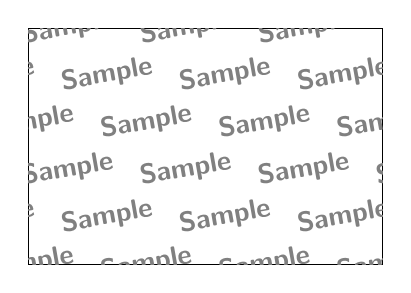
\begin{tikzpicture}
    \draw rectangle++(4.5,3);
    \clip rectangle++(4.5,3);
    \foreach\x in{0,1,2,3,4}{
      \foreach\y in{0,1,2,3,4,5,6}{
        \path(\x*1.5-\y*0.5,\y*0.6)node[rotate=10,text=gray]{\sffamily\bfseries\itshape Sample };
      }
    }
  \end{tikzpicture}
  %% 入れる画像：slam_toolbox で turtlebot3_world の地図を作っている途中の RViz2 の画面（Map・LaserScan・RobotModel を表示）のスクリーンショット
  % eps 画像を貼る場合は includegraphics をお使いください。
  % 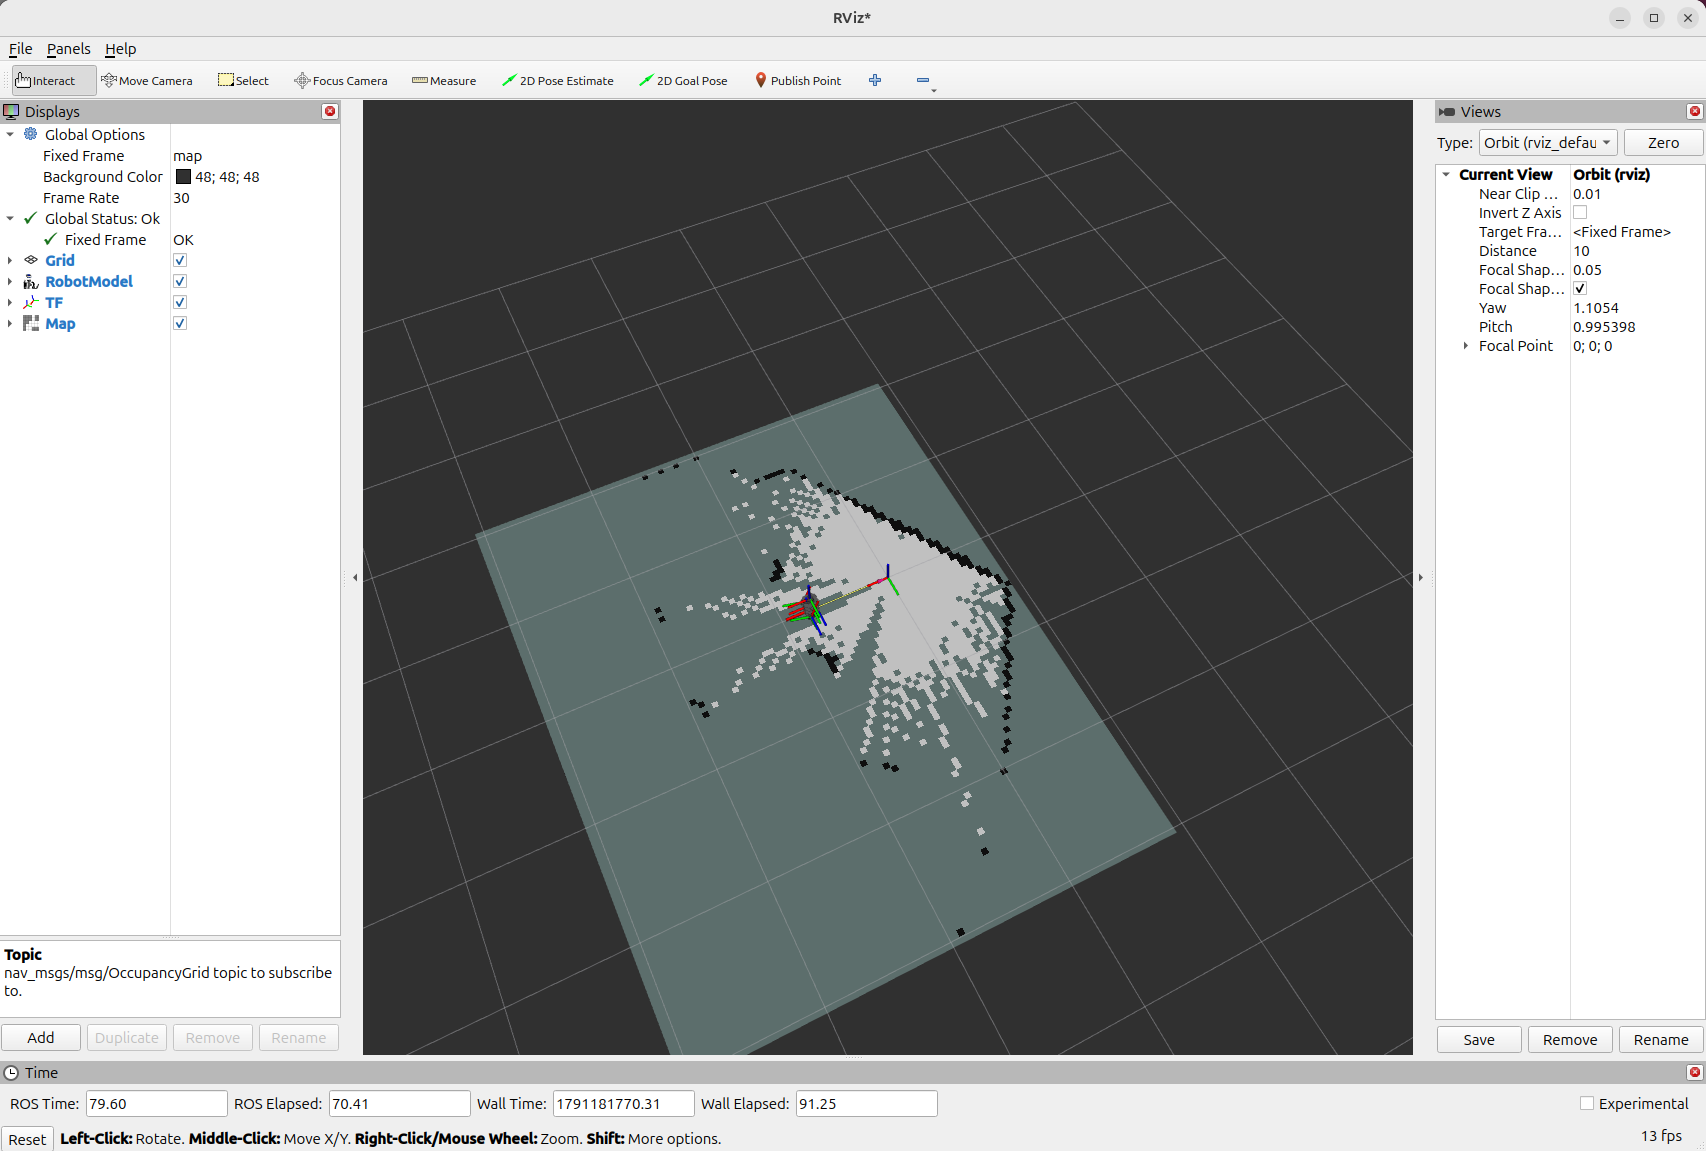
\includegraphics[width=0.8\linewidth]{practice/slam.png}
  \caption{SLAM で地図を作っている様子}
  \label{fig:practice-slam}
\end{figure}

\begin{point}[きれいな地図を作るコツ]
  \begin{itemize}
    \item ゆっくり動かす。特に、その場での回転は、ゆっくり行う
    \item 同じ場所を何度か通り、ぐるりと 1 周して出発した場所に戻ってくる（ループを閉じる）と、ずれが補正されて地図がきれいになる
    \item 障害物が少なく、特徴のない長い廊下などでは、地図がずれやすい
  \end{itemize}
\end{point}

\subsection{地図を保存する}

地図ができたら、ファイルに保存します。
Navigation2 の \cmd{map\_saver\_cli} を使います。

\begin{terminal}[地図を保存する]
~/ros2_ws$ sudo apt install ros-jazzy-navigation2 ros-jazzy-nav2-bringup
~/ros2_ws$ ros2 run nav2_map_server map_saver_cli -f ~/map --ros-args -p use_sim_time:=true
...
[INFO] [...] [map_saver]: Map saved successfully
~/ros2_ws$ ls ~/map.*
/home/user/map.pgm  /home/user/map.yaml
\end{terminal}

\cmd{map.pgm} は地図の画像、\cmd{map.yaml} は地図の大きさ（1 ピクセルが何メートルか）や原点の位置などを書いた設定ファイルです。
次の節で、この地図を使います。
保存したら、slam\_toolbox と RViz2 は止めておきましょう。

\section{Navigation2 による自律移動の体験}
\label{sec:practice-nav2}

\subsection{Navigation2 とは}

\textbf{Navigation2}（Nav2）は、移動ロボットを、地図の上の目的地まで自動で移動させるためのパッケージの集まりです。
目的地を指示すると、次のようなことを行ってくれます。

\begin{description}
  \item[自己位置推定] 保存した地図と LiDAR のデータを照らし合わせて、地図の上でのロボットの位置を推定します（AMCL というしくみを使います）。
  \item[経路計画] 地図の上で、今の位置から目的地までの経路を計画します。
  \item[経路追従と障害物回避] 計画した経路に沿って進むように、速度の指令を出します。地図にない障害物（人や箱など）が現れたら、それを避けます。
  \item[リカバリ] 行き詰まったときに、少し下がったり回ったりして、抜け出そうとします。
\end{description}

\subsection{自律移動させる}

TurtleBot3 には、Navigation2 を TurtleBot3 用の設定で起動する launch ファイルが用意されています。
シミュレーションを起動したまま、前の節で保存した地図を指定して起動します。

\begin{terminal}[Navigation2 を起動する]
~/ros2_ws$ ros2 launch turtlebot3_navigation2 navigation2.launch.py use_sim_time:=True map:=$HOME/map.yaml
\end{terminal}

Navigation2 の設定が済んだ RViz2 が、一緒に起動します。
次の手順で、ロボットを動かしてみましょう。

\begin{enumerate}
  \item \textbf{初期位置を教える}：RViz2 の上のツールバーの「2D Pose Estimate」を押し、地図の上でロボットがいる位置をクリックして、そのままロボットが向いている方向にドラッグします。LiDAR の点が地図の壁や柱と重なれば、うまく位置を教えられています。
  \item \textbf{目的地を指示する}：ツールバーの「Nav2 Goal」を押し、地図の上の行きたい場所をクリックして、着いたときに向いていてほしい方向にドラッグします。
\end{enumerate}

ロボットが経路を計画し、柱を避けながら、目的地まで自動で移動します（図\ref{fig:practice-nav2}）。
RViz2 には、計画した経路や、障害物の周りの「近づかないほうがよい範囲」（\textbf{コストマップ}）が色付きで表示されます。

\begin{figure}[tb]
  \centering
  \large
  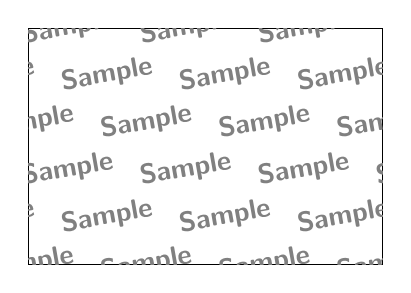
\begin{tikzpicture}
    \draw rectangle++(4.5,3);
    \clip rectangle++(4.5,3);
    \foreach\x in{0,1,2,3,4}{
      \foreach\y in{0,1,2,3,4,5,6}{
        \path(\x*1.5-\y*0.5,\y*0.6)node[rotate=10,text=gray]{\sffamily\bfseries\itshape Sample };
      }
    }
  \end{tikzpicture}
  %% 入れる画像：turtlebot3_navigation2 の RViz2 で、Nav2 Goal を指示し、計画された経路とコストマップが表示されている画面のスクリーンショット
  % eps 画像を貼る場合は includegraphics をお使いください。
  % \includegraphics[width=0.8\linewidth]{practice/nav2.png}
  \caption{Navigation2 で目的地まで自律移動している様子}
  \label{fig:practice-nav2}
\end{figure}

\subsection{目的地はアクションで指示する}

「Nav2 Goal」で目的地を指示したとき、裏では、\ref{sec:ros2-concepts-action}節で学んだ\textbf{アクション}が使われています。
目的地までの移動は時間がかかり、途中経過（残りの距離など）を知りたく、途中でキャンセルもしたいので、アクションがぴったりなのです。
アクションの一覧を見てみましょう。

\begin{terminal}[Navigation2 のアクションを調べる]
~/ros2_ws$ ros2 action list
...
/navigate_to_pose
...
\end{terminal}

\cmd{/navigate\_to\_pose} が、目的地まで移動させるアクションです。
コマンドから、ゴールを送ってみましょう。
\cmd{orientation} の \cmd{w: 1.0} は、地図の x 軸の方向（ヨーが 0）を向くという意味です（クォータニオン、\ref{sec:tf-viz-tf2}節）。

\begin{terminal}[コマンドから目的地を指示する]
~/ros2_ws$ ros2 action send_goal /navigate_to_pose nav2_msgs/action/NavigateToPose "{pose: {header: {frame_id: map}, pose: {position: {x: 1.0, y: 0.5}, orientation: {w: 1.0}}}}" --feedback
\end{terminal}

ロボットが地図の (1.0, 0.5) の位置に向かって移動し、途中経過として、残りの距離などがフィードバックで表示されます。
つまり、\ref{sec:rclpy-action}節で書いたアクションクライアントと同じようにノードを書けば、自分のプログラムからロボットを好きな場所に移動させられる、ということです。
Python から Navigation2 を使うための、\cmd{nav2\_simple\_commander} という便利なライブラリも用意されています。

\section{次のステップへ}
\label{sec:practice-next}

この本で学んだことを使えば、ロボットのソフトウェア開発の基本的な流れは、ひととおり体験できたことになります。
最後に、この先に進むための道しるべを紹介します。

\subsection{実際のロボットを動かす}

この章では、シミュレーションで TurtleBot3 を動かしました。
次の\ref{chap:kachaka}章では、家庭用ロボットのカチャカを使って、実際のロボットを動かします。
TurtleBot3 の実機では、ロボットに載っているコンピュータ（Raspberry Pi）で、モータと LiDAR を動かすノードを起動し、パソコンとはネットワーク（\ref{sec:ros2-install-network}節）でつながります。
あとは、この章とほぼ同じコマンドで、地図を作り、自律移動させられます。
実際のロボットでは、シミュレーションにはなかった問題（センサの雑音、車輪のすべり、ネットワークの遅れ、バッテリ切れ……）にたくさん出会うはずです。
それらに一つ一つ向き合うことが、ロボット開発のいちばん面白いところでもあります。

\subsection{さらに学ぶ}

興味に合わせて、次のようなテーマに進んでみましょう。

\begin{description}
  \item[ロボットアーム] ROS 2 でアームを動かすには、動作計画のフレームワーク \textbf{MoveIt 2} がよく使われます。
  \item[画像処理と認識] カメラの画像を OpenCV で処理したり、深層学習で物体を認識したりして、その結果を ROS 2 のノードで使います。
  \item[C++] 速さが求められるノードを書くために、C++ と rclcpp を学びましょう（補章\ref{sup:rclcpp}）。
  \item[マイコン] \textbf{micro-ROS} を使うと、マイコン（\ref{chap:computer}章）の上でも ROS 2 のノードを動かせます。
  \item[ロボットの理論] 座標変換、自己位置推定、経路計画、制御などの理論を学ぶと、パッケージが中で何をしているのかがわかり、自分で改良できるようになります。
\end{description}

\subsection{コミュニティに参加する}

ROS 2 は、世界中の人が開発しているオープンソースソフトウェアです（\ref{sec:linux-oss}節）。
ROS 2 の公式のドキュメントや、質問のためのフォーラムなど、学ぶための場所がたくさんあります（付録\ref{app:references}）。
わからないことを質問するときは、何をしたのか、何が起きたのか、エラーメッセージ、使っている環境（Ubuntu と ROS 2 のバージョン）を、ほかの人が再現できるように書きましょう。

慣れてきたら、使っているパッケージの不具合を Issue で報告したり、ドキュメントの誤りを直す Pull Request を送ったりしてみましょう（\ref{sec:git-github}節）。
小さな貢献でも、世界中のロボット開発者の役に立ちます。
ロボットの大会（競技会）に参加して、仲間と一緒にロボットを作るのも、力を伸ばすよい機会です。

この本が、あなたがロボットを動かすための、最初の一歩になれば幸いです。

\section*{この章のまとめ}

\begin{itemize}
  \item teleop\_twist\_keyboard を使うと、\cmd{/cmd\_vel} で動くどんな移動ロボットも、キーボードで操作できます。
  \item LiDAR のデータ（\cmd{/scan}）を読んで速度の指令（\cmd{/cmd\_vel}）を出すノードで、障害物を避けながら走らせられます。
  \item SLAM（slam\_toolbox）で、ロボットを動かしながら地図を作り、\cmd{map\_saver\_cli} で保存できます。
  \item Navigation2 は、地図の上での自己位置推定・経路計画・障害物回避を行い、ロボットを目的地まで自律移動させます。目的地はアクションで指示します。
  \item 実際のロボット、さらに進んだテーマ、コミュニティへの参加へと、次のステップに進みましょう。
\end{itemize}


% 補章（本編の内容を別の書き方などで補う章）
\hoshou
% 第V部の中に入らないように、番号なしの部として目次に載せる
\clearpage\phantomsection\addcontentsline{toc}{part}{補章}
\part*{補章}
\chapter{C++ でノードを書く（rclcpp）}
\label{sup:rclcpp}

\ref{chap:rclpy}章では、Python でノードを書きました。
ROS 2 のノードは、C++ でも書けます。
C++ でノードを書くためのライブラリを \textbf{rclcpp}（ROS Client Library for C++）といいます。
この補章では、\ref{chap:rclpy}章で作ったノードのいくつかを C++ で書き直しながら、rclcpp の書き方を説明します。
\ref{chap:rclpy}章の各節と見比べながら読んでください。

この補章のファイルは、サンプルコードの \cmd{ros2\_ws/src/}\allowbreak\cmd{my\_cpp\_package/} にあります。

\section{C++ と rclcpp}
\label{sec:rclcpp-intro}

\subsection{なぜ C++ で書くのか}

\ref{sec:python-vs-c}節で学んだように、C++ は、プログラムを実行する前にコンパイル（ビルド）が必要で、書く量も Python より多くなります。
その代わり、プログラムが速く動き、メモリの使い方も細かく決められます。
そのため、ROS 2 では、次のようなノードを C++ で書くことがよくあります。

\begin{itemize}
  \item カメラの画像や、LiDAR の点群など、大きなデータを処理するノード
  \item モータの制御のように、短い周期で、決まった時間内に処理を終える必要があるノード
  \item ROS 2 本体や、Navigation2 などの主要なパッケージ（多くが C++ で書かれています）
\end{itemize}

一方、試しに動かしてみるノードや、処理の重くないノードは、Python で手早く書くのが便利です。
ROS 2 では、トピックの名前と型が同じなら、C++ のノードと Python のノードが問題なく通信できるので、ノードごとに向いている言語を選べます。

\subsection{C++ の文法の最小限}

この本では C++ の文法は詳しく扱いませんが、この補章のプログラムを読むために、Python との主な違いを紹介しておきます。

\begin{tablebox}[Python と C++ の主な違い][tab:rclcpp-syntax]
  \begin{tabular}{p{0.2\linewidth}p{0.33\linewidth}p{0.36\linewidth}}
    \toprule
     & Python & C++ \\
    \midrule
    ブロック & インデントで表す & \cmd{\{ \}} で囲む \\
    文の終わり & 改行 & \cmd{;}（セミコロン） \\
    変数 & 型を書かない & 型を書く（\cmd{int count;}）。\cmd{auto} と書くと型を自動で決める \\
    読み込み & \cmd{import} & \cmd{\#include} \\
    コメント & \cmd{\#} & \cmd{//} \\
    名前の区切り & \cmd{rclpy.node} & \cmd{rclcpp::Node}（\cmd{::} で区切る） \\
    自分自身 & \cmd{self} & \cmd{this}（省略できることが多い） \\
    \bottomrule
  \end{tabular}
\end{tablebox}

C++ のプログラムは、\cmd{main} という名前の関数から実行が始まります。
Python の \cmd{if \_\_name\_\_ == '\_\_main\_\_':}（\ref{sec:python-class-module}節）にあたるものです。

\section{パッケージを作る}
\label{sec:rclcpp-package}

C++ のノードは、\cmd{ament\_cmake} のパッケージに入れます（\ref{sec:workspace-create}節）。
\cmd{--dependencies} で、使うパッケージも指定しておきます。

\begin{terminal}[C++ のパッケージを作る]
$ cd ~/ros2_ws/src
~/ros2_ws/src$ ros2 pkg create --build-type ament_cmake --license Apache-2.0 --dependencies rclcpp std_msgs geometry_msgs turtlesim example_interfaces my_cpp_package
\end{terminal}

\begin{terminal}[C++ のパッケージの中身]
~/ros2_ws/src$ tree my_cpp_package
my_cpp_package
├── CMakeLists.txt
├── include
│   └── my_cpp_package
├── package.xml
└── src
\end{terminal}

\begin{description}
  \item[\cmd{src/}] ノードのソースファイル（\cmd{.cpp}）を置きます。
  \item[\cmd{include/}] ほかのファイルやパッケージから使うヘッダファイル（\cmd{.hpp}）を置きます。この補章では使いません。
  \item[\cmd{CMakeLists.txt}] ビルドの方法を書くファイルです（\ref{sec:rclcpp-build}節）。Python のパッケージの \cmd{setup.py} にあたります。
  \item[\cmd{package.xml}] Python のパッケージと同じく、パッケージの情報と依存関係を書きます。\cmd{--dependencies} で指定したパッケージが、\cmd{<depend>} として書き込まれています。
\end{description}

\section{はじめてのノード}
\label{sec:rclcpp-first}

\subsection{ノードのプログラム}

\ref{sec:rclpy-first}節の \cmd{hello\_node.py} を C++ で書くと、次のようになります。
\cmd{src} の中に \cmd{hello\_node.cpp} を作ります。

\codefile[style=cpp]{はじめてのノード（src/hello\_node.cpp）}{lst:rclcpp-hello}{samples/rclcpp/my_cpp_package/src/hello_node.cpp}

\begin{description}
  \item[3 行目] rclcpp を読み込みます。
  \item[5 行目] \cmd{rclcpp::Node} クラスを継承して、\cmd{HelloNode} クラスを作ります。C++ では、\cmd{class クラス名 : public 親クラス} と書きます。
  \item[7 行目] \cmd{public:} の後に書いたものは、クラスの外から使えます。
  \item[8〜12 行目] クラスと同じ名前の関数は、\textbf{コンストラクタ}といい、Python の \cmd{\_\_init\_\_} にあたります。9 行目の \cmd{: Node("hello\_node")} で、親クラスにノードの名前を渡しています（Python の \cmd{super().\_\_init\_\_('hello\_node')} にあたります）。
  \item[11 行目] \cmd{RCLCPP\_INFO} で、ログを出力します。Python の \cmd{get\_logger().info()} にあたります。
  \item[17〜19 行目] rclcpp の準備（\cmd{init}）、ノードを作って動かし続ける（\cmd{spin}）、終了（\cmd{shutdown}）という流れは、Python と同じです。\cmd{std::make\_shared<HelloNode>()} は、\cmd{HelloNode} のインスタンスを作る書き方です（後のポイントで説明します）。
\end{description}

Python と違い、\key{Ctrl}+\key{C} を受け止める \cmd{try} を書く必要はありません。
\key{Ctrl}+\key{C} が押されると、\cmd{rclcpp::spin()} が終わり、そのまま \cmd{shutdown()} に進みます。

\section{ビルドの設定}
\label{sec:rclcpp-build}

\subsection{CMakeLists.txt}

C++ のノードは、ソースファイルから実行ファイルを作る（コンパイルする）必要があります。
その方法を \cmd{CMakeLists.txt} に書きます。
この補章のすべてのノードをビルドする \cmd{CMakeLists.txt} は、次のとおりです。

\codefile[style=bash]{my\_cpp\_package/CMakeLists.txt}{lst:rclcpp-cmake}{samples/rclcpp/my_cpp_package/CMakeLists.txt}

\begin{description}
  \item[\cmd{find\_package}] 使うパッケージを探します。\cmd{package.xml} に書いたパッケージを、ここにも書きます。
  \item[\cmd{add\_executable}] ソースファイルから、実行ファイルを作ります。最初に書いた名前（\cmd{hello\_node}）が、\cmd{ros2 run} で指定する名前になります。
  \item[\cmd{ament\_target\_dependencies}] その実行ファイルが使うパッケージを指定します。
  \item[\cmd{install}] 作った実行ファイルを、\cmd{install} ディレクトリにコピーします。
\end{description}

新しいノードを追加したときは、\cmd{add\_executable}・\cmd{ament\_target\_dependencies}・\cmd{install} の 3 か所に書き加えます。
Python のパッケージで、\cmd{setup.py} の \cmd{entry\_points} に 1 行追加したのにあたる作業です。

\subsection{ビルドして実行する}

\begin{terminal}[C++ のノードをビルドして実行する]
~/ros2_ws/src$ cd ~/ros2_ws
~/ros2_ws$ colcon build --packages-select my_cpp_package
Starting >>> my_cpp_package
Finished <<< my_cpp_package [35.2s]

Summary: 1 package finished [35.5s]
~/ros2_ws$ source install/local_setup.bash
~/ros2_ws$ ros2 run my_cpp_package hello_node
[INFO] [1727852400.123456789] [hello_node]: こんにちは、ROS 2!
\end{terminal}

Python のパッケージより、ビルドに時間がかかることがわかります。
また、C++ では、\textbf{ソースファイルを書き換えるたびにビルドし直す必要があります}。
\cmd{--symlink-install} を付けても、ビルドしないと変更は反映されません。

\begin{caution}[ビルドのエラーを読む]
  C++ では、文法の誤りや型の間違いは、実行する前の、ビルドのときにエラーとして見つかります。
  エラーが出たら、\ref{sec:python-class-debug}節と同じく、最初のエラーメッセージから読みましょう。
  \cmd{src/talker.cpp:19:5: error: ...} のように、ファイル名・行番号・列番号が表示されます。
  1 つの誤りから、たくさんのエラーが続けて表示されることもあるので、まず一番上のエラーを直してから、ビルドし直すのがコツです。
\end{caution}

\section{パブリッシャとサブスクライバ}
\label{sec:rclcpp-pubsub}

\subsection{パブリッシャ}

\ref{sec:rclpy-pubsub}節の \cmd{talker.py} を C++ で書くと、次のようになります。
\cmd{main} 関数は、作るノードのクラスの名前が違うだけで、\ref{sec:rclcpp-first}節と同じ形です。

\codefile[style=cpp]{パブリッシャ（src/talker.cpp）}{lst:rclcpp-talker}{samples/rclcpp/my_cpp_package/src/talker.cpp}

\begin{description}
  \item[6 行目] メッセージ型 \cmd{std\_msgs/msg/String} を読み込みます。C++ では、\cmd{パッケージ名/msg/型の名前.hpp} を \cmd{\#include} します。ファイル名は、型の名前を小文字とアンダースコアにしたものです（\cmd{RobotStatus} なら \cmd{robot\_status.hpp}）。
  \item[8 行目] \cmd{500ms} や \cmd{1s} のように、時間を単位付きで書けるようにします。
  \item[14 行目] \cmd{count\_(0)} で、メンバ変数（Python の \cmd{self.count}）の初期値を決めています。
  \item[17 行目] パブリッシャを作ります。メッセージ型は \cmd{<>} の中に書きます。
  \item[19 行目] タイマを作ります。\cmd{std::bind(\&Talker::timer\_callback, this)} は、「このノード（\cmd{this}）の \cmd{timer\_callback} を呼び出す」という関数を作る書き方で、Python の \cmd{self.timer\_callback} にあたります。
  \item[22 行目] \cmd{private:} の後に書いたものは、クラスの中からだけ使えます。
  \item[32〜34 行目] パブリッシャ・タイマ・カウンタを、メンバ変数として宣言します。C++ では、メンバ変数もここで型を書いて宣言しておく必要があります。名前の最後の \cmd{\_} は、メンバ変数であることを示すための習慣です。
\end{description}

\cmd{publisher\_->publish(msg)} の \cmd{->} は、後のポイントで説明する「スマートポインタ」の先にあるものを使うときの書き方です。
\cmd{RCLCPP\_INFO} は、C 言語の \cmd{printf} と同じく、\cmd{\%s}（文字列）や \cmd{\%d}（整数）、\cmd{\%.1f}（小数）の部分に、後ろの値を埋め込んで表示します。

\begin{point}[SharedPtr と make\_shared]
  rclcpp では、ノードやパブリッシャなどを、\textbf{スマートポインタ}（\cmd{std::shared\_ptr}）で扱います。
  \textbf{ポインタ}は、データそのものではなく、データがメモリのどこにあるかを指し示す値です。
  スマートポインタは、そのデータを誰も使わなくなったら、自動でメモリを片付けてくれる、便利なポインタです。
  \begin{itemize}
    \item \cmd{〇〇::SharedPtr} は、\cmd{〇〇} を指すスマートポインタの型です。
    \item \cmd{std::make\_shared<クラス>()} で、インスタンスを作り、それを指すスマートポインタを受け取ります。
    \item スマートポインタの先にあるメソッドや変数は、\cmd{.} ではなく \cmd{->} で使います（\cmd{publisher\_->publish(msg)}）。
  \end{itemize}
  Python では、すべての値がこれと似たしくみで扱われているので、意識する必要がありませんでした。
\end{point}

\subsection{サブスクライバ}

\ref{sec:rclpy-pubsub}節の \cmd{listener.py} を C++ で書くと、次のようになります。

\codefile[style=cpp]{サブスクライバ（src/listener.cpp）}{lst:rclcpp-listener}{samples/rclcpp/my_cpp_package/src/listener.cpp}

コールバックには、届いたメッセージが引数として渡されるので、\cmd{std::bind} に \cmd{std::placeholders::\_1}（「1 つ目の引数をここに渡す」という意味）を付けます。
コールバックの引数の \cmd{const std\_msgs::msg::String \& msg} は、「メッセージをコピーせずに、変更しない約束で受け取る」という意味です。
大きなメッセージでもコピーしないので、速く処理できます。

ビルドして、C++ の talker と、\ref{chap:rclpy}章の Python の listener を組み合わせてみましょう。

\begin{terminal}[C++ のノードと Python のノードで通信する]
$ ros2 run my_cpp_package talker   # 1 つ目のターミナル
$ ros2 run my_package listener     # 2 つ目のターミナル
[INFO] [...] [listener]: I heard: "Hello, ROS 2! 3"
...
\end{terminal}

C++ で書いたノードと Python で書いたノードが、問題なく通信できることがわかります。

\section{タイマとコールバック}
\label{sec:rclcpp-timer}

\ref{sec:rclpy-timer}節の \cmd{turtle\_controller.py} を C++ で書くと、次のようになります。

\codefile[style=cpp]{カメを自動で動かすノード（src/turtle\_controller.cpp）}{lst:rclcpp-turtle-controller}{samples/rclcpp/my_cpp_package/src/turtle_controller.cpp}

構成は Python とまったく同じです。
Python では、まだ位置が届いていないことを \cmd{None}（\ref{sec:python-basics-none}節）で表しましたが、C++ では \cmd{std::optional} を使っています。
\cmd{std::optional<型>} は「値があるか、値がないか」のどちらかを持てる型で、\cmd{if (!pose\_)} で値がないことを調べ、\cmd{pose\_->x} で中の値を使います。

\begin{terminal}[C++ のノードで turtlesim を動かす]
$ ros2 run turtlesim turtlesim_node             # 1 つ目のターミナル
$ ros2 run my_cpp_package turtle_controller     # 2 つ目のターミナル
\end{terminal}

\section{サービスサーバ}
\label{sec:rclcpp-service}

\ref{sec:rclpy-service}節の \cmd{add\_two\_ints\_server.py} を C++ で書くと、次のようになります。

\codefile[style=cpp]{サービスサーバ（src/add\_two\_ints\_server.cpp）}{lst:rclcpp-service-server}{samples/rclcpp/my_cpp_package/src/add_two_ints_server.cpp}

\cmd{using AddTwoInts = ...} は、長い型の名前に、短い別名を付ける書き方です。
サービスのコールバックは、リクエストとレスポンスの 2 つを受け取るので、\cmd{std::placeholders::\_1} と \cmd{\_2} を付けます。
Python ではレスポンスを \cmd{return} しましたが、C++ では、受け取ったレスポンスに値を入れるだけで、クライアントに返されます。

\cmd{ros2 service call} で呼び出せば、\ref{sec:rclpy-service}節の Python のサーバと同じ結果が返ってきます。
サービスクライアントやアクションも C++ で書けますが、書き方が少し複雑になるので、この本では省略します。
ROS 2 の公式のチュートリアル（付録\ref{app:references}）に、C++ での書き方が載っています。

\section{パラメータ}
\label{sec:rclcpp-param}

\ref{sec:rclpy-param}節の \cmd{param\_node.py} を C++ で書くと、次のようになります。

\codefile[style=cpp]{パラメータを使うノード（src/param\_node.cpp）}{lst:rclcpp-param}{samples/rclcpp/my_cpp_package/src/param_node.cpp}

パラメータの宣言は、Python と同じく、名前と初期値を渡します。
値を取得するときは、\cmd{as\_string()} や \cmd{as\_double()} のように、型を指定して取り出します。
C++ では、変数にも型があるので、取り出す型と変数の型をそろえる必要があります。

起動のときの \cmd{-p} や、\cmd{ros2 param set} での変更も、Python のノードとまったく同じように使えます。
launch ファイル（\ref{chap:launch}章）からも、Python のノードと同じように起動し、パラメータを設定できます。

\section{Python と C++ の対応}
\label{sec:rclcpp-summary}

この補章で使った書き方と、\ref{chap:rclpy}章の Python の書き方の対応をまとめておきます。

\begin{tablebox}[rclpy と rclcpp の対応][tab:rclcpp-compare]
  \begin{tabular}{ll}
    \toprule
    rclpy（Python） & rclcpp（C++） \\
    \midrule
    \cmd{from std\_msgs.msg import String} & \cmd{\#include "std\_msgs/msg/string.hpp"} \\
    \cmd{class Talker(Node):} & \cmd{class Talker : public rclcpp::Node} \\
    \cmd{super().\_\_init\_\_('talker')} & \cmd{: Node("talker")} \\
    \cmd{self.get\_logger().info(...)} & \cmd{RCLCPP\_INFO(get\_logger(), ...)} \\
    \cmd{create\_publisher(String, ...)} & \cmd{create\_publisher<std\_msgs::msg::String>(...)} \\
    \cmd{create\_timer(0.5, ...)} & \cmd{create\_wall\_timer(500ms, ...)} \\
    \cmd{self.timer\_callback} & \cmd{std::bind(\&Talker::timer\_callback, this)} \\
    \cmd{None} & \cmd{std::optional} \\
    \cmd{get\_parameter(...).value} & \cmd{get\_parameter(...).as\_double()} など \\
    \cmd{setup.py} の \cmd{entry\_points} & \cmd{CMakeLists.txt} の \cmd{add\_executable} など \\
    \bottomrule
  \end{tabular}
\end{tablebox}

文法は違いますが、「\cmd{Node} を継承したクラスを作り、コンストラクタでパブリッシャ・サブスクライバ・タイマなどを作って、あとはコールバックで処理する」という構成は、Python と C++ でまったく同じです。
rclpy で考え方を身につけておけば、rclcpp で書かれたノードも読めるようになります。
C++ の文法をもっと学びたい人は、C++ の入門書と、ROS 2 の公式のチュートリアルを合わせて読むのがおすすめです。

\chapter{XML による launch ファイルの書き方}
\label{sup:launch-xml}

\ref{chap:launch}章では、Python で launch ファイルを書きました。
launch ファイルは、XML の形式でも書けます。
この補章では、\ref{chap:launch}章で作った 5 つの launch ファイルを XML で書き直しながら、XML の launch ファイルの書き方を説明します。
\ref{chap:launch}章の各節と見比べながら読んでください。
ここで紹介するファイルは、サンプルコードの \cmd{ros2\_ws/src/}\allowbreak\cmd{my\_package/launch/} に、Python のファイルと並べて置いてあります。

\section{XML の launch ファイルの特徴}
\label{sec:launch-xml-feature}

\subsection{Python と XML の比べ方}

XML は、\cmd{<タグ>} で囲んで情報を書く形式です。
\cmd{package.xml}（\ref{sec:workspace-files}節）も XML で書かれていました。
XML の launch ファイルには、Python の launch ファイルと比べて、次のような特徴があります。

\begin{tablebox}[Python と XML の launch ファイルの比較][tab:launch-xml-compare]
  \begin{tabular}{lp{0.36\linewidth}p{0.36\linewidth}}
    \toprule
     & Python & XML \\
    \midrule
    ファイル名 & \cmd{〇〇.launch.py} & \cmd{〇〇.launch.xml} \\
    書く量 & \cmd{import} などが必要で、長くなりがち & 短く書ける \\
    読みやすさ & Python を知っていれば読める & 何を起動するかが一目でわかる \\
    柔軟さ & for 文や if 文など、プログラムとして自由に書ける & 決まったタグの組み合わせで書く \\
    \bottomrule
  \end{tabular}
\end{tablebox}

ノードを並べて起動するだけの単純な launch ファイルなら、XML のほうが短く、読みやすく書けます。
一方、起動するノードを計算で決めるなど、複雑なことをしたい場合は、Python のほうが向いています。
ROS 2 では、どちらの形式も同じように使え、Python の launch ファイルから XML の launch ファイルを読み込む（あるいはその逆の）こともできます。

\subsection{インストールの設定}

XML の launch ファイルも、Python の launch ファイルと同じく、パッケージの \cmd{launch} ディレクトリに置き、\cmd{setup.py} の \cmd{data\_files} でインストールします（\ref{sec:launch-python}節）。
\cmd{glob('launch/*.launch.*')} と書いておけば、\cmd{.launch.py} と \cmd{.launch.xml} の両方がインストールされます。
実行の仕方も同じで、\cmd{ros2 launch パッケージ名 ファイル名} で実行します。

\begin{terminal}[XML の launch ファイルを実行する]
$ ros2 launch my_package turtlesim_controller.launch.xml
\end{terminal}

\section{ノードを起動する}
\label{sec:launch-xml-node}

\subsection{node タグ}

\ref{sec:launch-python}節の \cmd{turtlesim\_controller.launch.py} を XML で書くと、次のようになります。

\lstinputlisting[style=xml, caption={launch/turtlesim\_controller.launch.xml}, label={lst:launch-xml-first}]{samples/rclpy/my_package/launch/turtlesim_controller.launch.xml}

全体を \cmd{<launch>} と \cmd{</launch>} で囲み、その中に、起動するノードを \cmd{<node>} タグで 1 つずつ書きます。
中身のないタグは、\cmd{<node ... />} のように、最後を \cmd{/>} で閉じます。
\cmd{<!-{}- -{}->} で囲んだ部分は、XML のコメントです。

\cmd{<node>} タグの属性（\cmd{名前="値"} の部分）は、Python の \cmd{Node} の引数に対応しています。
名前が少し違うものがあるので注意しましょう。

\begin{tablebox}[node タグの主な属性][tab:launch-xml-node]
  \begin{tabular}{llp{0.42\linewidth}}
    \toprule
    XML の属性 & Python の引数 & 意味 \\
    \midrule
    \cmd{pkg} & \cmd{package} & パッケージ名 \\
    \cmd{exec} & \cmd{executable} & 実行ファイルの名前 \\
    \cmd{name} & \cmd{name} & ノードの名前の付け替え \\
    \cmd{namespace} & \cmd{namespace} & 名前空間 \\
    \cmd{output} & \cmd{output} & \cmd{screen} でログをターミナルに表示 \\
    \bottomrule
  \end{tabular}
\end{tablebox}

\section{パラメータを設定する}
\label{sec:launch-xml-param}

\subsection{param タグ}

\ref{sec:launch-yaml}節の \cmd{param.launch.py} を XML で書くと、次のようになります。

\lstinputlisting[style=xml, caption={launch/param.launch.xml}, label={lst:launch-xml-param}]{samples/rclpy/my_package/launch/param.launch.xml}

パラメータは、\cmd{<node>} と \cmd{</node>} の間に、\cmd{<param>} タグで書きます。

\begin{itemize}
  \item \cmd{<param name="名前" value="値"/>}：パラメータを 1 つ設定します。
  \item \cmd{<param from="YAML ファイル"/>}：YAML ファイルからまとめて読み込みます。
\end{itemize}

Python と同じく、後に書いたものが優先されるので、\cmd{max\_speed} は \cmd{0.8} になります。

\subsection{置換式}

\cmd{\$(find-pkg-share my\_package)} の部分は、\textbf{置換式}といいます。
\cmd{ros2 launch} がファイルを読むときに、\cmd{\$( )} の部分を、計算した値に置き換えます。
\cmd{find-pkg-share} は、Python の \cmd{get\_package\_share\_directory()} と同じく、パッケージがインストールされた場所に置き換わります。
よく使う置換式は、次のとおりです。

\begin{tablebox}[よく使う置換式][tab:launch-xml-subst]
  \begin{tabular}{lp{0.55\linewidth}}
    \toprule
    置換式 & 置き換わる値 \\
    \midrule
    \cmd{\$(find-pkg-share パッケージ名)} & パッケージの \cmd{share} ディレクトリの場所 \\
    \cmd{\$(var 名前)} & launch 引数の値（\ref{sec:launch-xml-bringup}節） \\
    \cmd{\$(env 名前)} & 環境変数（\ref{chap:env}章）の値 \\
    \bottomrule
  \end{tabular}
\end{tablebox}

\section{名前空間とリマップ}
\label{sec:launch-xml-namespace}

\subsection{名前空間}

\ref{sec:launch-namespace}節の \cmd{multi\_turtles.launch.py} を XML で書くと、次のようになります。

\lstinputlisting[style=xml, caption={launch/multi\_turtles.launch.xml}, label={lst:launch-xml-multi}]{samples/rclpy/my_package/launch/multi_turtles.launch.xml}

\cmd{<group>} タグは、ノードをまとめるためのタグです。
\cmd{<group>} の中に \cmd{<push\_ros\_namespace>} を書くと、そのグループの中のすべてのノードが、指定した名前空間で起動します。
1 つのノードだけなら、\cmd{<node>} タグに \cmd{namespace} 属性を書いても構いません（次のリスト\ref{lst:launch-xml-mimic}）。

XML には for 文がないので、Python のように繰り返しを使って書くことはできず、2 組分をそのまま並べて書いています。
このように、同じものを何度も書く必要がある場合は、Python の launch ファイルのほうが便利です。

\subsection{リマップ}

\ref{sec:launch-namespace}節の \cmd{mimic.launch.py} を XML で書くと、次のようになります。

\lstinputlisting[style=xml, caption={launch/mimic.launch.xml}, label={lst:launch-xml-mimic}]{samples/rclpy/my_package/launch/mimic.launch.xml}

リマップは、\cmd{<node>} の中に \cmd{<remap from="元の名前" to="新しい名前"/>} と書きます。

\section{launch 引数とインクルード}
\label{sec:launch-xml-bringup}

\subsection{arg タグと include タグ}

\ref{sec:launch-bringup}節の \cmd{bringup.launch.py} を XML で書くと、次のようになります。
ここでは、XML の便利な機能を紹介するために、talker と listener を起動するかどうかを決める launch 引数 \cmd{use\_chatter} を追加しています。

\lstinputlisting[style=xml, caption={launch/bringup.launch.xml}, label={lst:launch-xml-bringup}]{samples/rclpy/my_package/launch/bringup.launch.xml}

\begin{description}
  \item[\cmd{<arg>}] launch 引数を宣言します。Python の \cmd{DeclareLaunchArgument} にあたります。\cmd{default} に省略したときの値、\cmd{description} に説明を書きます。
  \item[\cmd{\$(var 名前)}] launch 引数の値に置き換わります。Python の \cmd{LaunchConfiguration} にあたります。
  \item[\cmd{<include>}] ほかの launch ファイルを読み込みます。Python の \cmd{IncludeLaunchDescription} にあたります。読み込む launch ファイルは、Python・XML のどちらの形式でも構いません。
\end{description}

\subsection{条件によって起動する}

\cmd{<node>} タグや \cmd{<include>} タグ、\cmd{<group>} タグに \cmd{if="値"} を書くと、値が \cmd{true} のときだけ起動します。
反対に、\cmd{unless="値"} を書くと、値が \cmd{false} のときだけ起動します。
launch 引数と組み合わせると、起動するときに、起動するノードを切り替えられます。

\begin{terminal}[launch 引数で起動するノードを切り替える]
$ ros2 launch my_package bringup.launch.xml robot_name:=erasers use_chatter:=false
\end{terminal}

このように実行すると、talker と listener は起動しません。
Python の launch ファイルでも、\cmd{IfCondition} を使えば同じことができますが、XML のほうが短く書けます。

\section{XML の launch ファイルのまとめ}
\label{sec:launch-xml-summary}

この補章で使ったタグと、Python の launch ファイルとの対応をまとめておきます。

\begin{tablebox}[XML のタグと Python の launch ファイルの対応][tab:launch-xml-summary]
  \begin{tabular}{ll}
    \toprule
    XML & Python \\
    \midrule
    \cmd{<launch>} & \cmd{LaunchDescription} \\
    \cmd{<node>} & \cmd{Node} \\
    \cmd{<param name=... value=...>} & \cmd{parameters=[\{'名前': 値\}]} \\
    \cmd{<param from=...>} & \cmd{parameters=[YAML ファイル]} \\
    \cmd{<remap from=... to=...>} & \cmd{remappings=[(元, 新)]} \\
    \cmd{<group>} と \cmd{<push\_ros\_namespace>} & \cmd{GroupAction} と \cmd{PushRosNamespace} \\
    \cmd{<arg>} & \cmd{DeclareLaunchArgument} \\
    \cmd{\$(var 名前)} & \cmd{LaunchConfiguration('名前')} \\
    \cmd{<include>} & \cmd{IncludeLaunchDescription} \\
    \cmd{if="..."}, \cmd{unless="..."} & \cmd{IfCondition}, \cmd{UnlessCondition} \\
    \bottomrule
  \end{tabular}
\end{tablebox}

\begin{point}[YAML の launch ファイル]
  launch ファイルは、YAML の形式（\cmd{〇〇.launch.yaml}）でも書けます。
  使えるタグ（キー）は XML とほぼ同じで、たとえば \cmd{<node pkg="turtlesim" exec="turtlesim\_node"/>} は、次のように書きます。
\begin{lstlisting}[numbers=none, xleftmargin=0pt, framexleftmargin=0pt]
launch:
  - node:
      pkg: turtlesim
      exec: turtlesim_node
\end{lstlisting}
  公開されているパッケージでは、Python と XML の launch ファイルがよく使われ、YAML の launch ファイルはあまり見かけません。
\end{point}


\appendix
\clearpage\phantomsection\addcontentsline{toc}{part}{付録}
\part*{付録}
\chapter{コマンド早見表}
\label{app:cheatsheet}

本書で使った主なコマンドを、目的ごとにまとめました。
詳しい使い方は、各章の本文か、\cmd{man コマンド名} や \cmd{コマンド名 --help}（\ref{sec:terminal-help}節）で調べてください。
「〇〇」の部分は、ファイル名やパッケージ名などに置き換えて使います。

\section{Linux の基本}
\label{sec:cheatsheet-linux}

Linux の基本的な操作のコマンドです。

\begin{tablebox}[ヘルプと履歴（第4章）][tab:cheatsheet-help]
  \begin{tabular}{p{0.38\linewidth}p{0.52\linewidth}}
    \toprule
    コマンド & 意味 \\
    \midrule
    \cmd{man 〇〇} & コマンドのマニュアルを表示する（\key{q} で終了） \\
    \cmd{〇〇 --help} & コマンドの簡単な使い方を表示する \\
    \cmd{history} & 入力したコマンドの履歴を表示する \\
    \cmd{clear} & 画面をきれいにする \\
    \bottomrule
  \end{tabular}
\end{tablebox}

\begin{tablebox}[ファイルとディレクトリ（第5章）][tab:cheatsheet-files]
  \begin{tabular}{p{0.38\linewidth}p{0.52\linewidth}}
    \toprule
    コマンド & 意味 \\
    \midrule
    \cmd{pwd} & 今いるディレクトリを表示する \\
    \cmd{ls -la} & 隠しファイルも含めて、詳しく一覧を表示する \\
    \cmd{cd 〇〇} / \cmd{cd \textasciitilde} / \cmd{cd ..} & 移動する / ホームへ / 1 つ上へ \\
    \cmd{mkdir -p 〇〇/〇〇} & ディレクトリを（途中のものも）作る \\
    \cmd{touch 〇〇} & 空のファイルを作る \\
    \cmd{cp 元 先} / \cmd{cp -r 元 先} & ファイルを / ディレクトリごとコピーする \\
    \cmd{mv 元 先} & 移動する・名前を変える \\
    \cmd{rm 〇〇} / \cmd{rm -r 〇〇} & ファイルを / ディレクトリごと削除する（元に戻せない） \\
    \cmd{cat 〇〇} & ファイルの中身を表示する \\
    \cmd{less 〇〇} & ファイルを 1 画面ずつ表示する（\key{q} で終了） \\
    \cmd{head -n 5 〇〇} / \cmd{tail -n 5 〇〇} & 先頭 / 末尾の 5 行を表示する \\
    \cmd{tail -f 〇〇} & ファイルに追加される内容を表示し続ける \\
    \cmd{find . -name "*.py"} & 名前でファイルを探す \\
    \cmd{tree} & ディレクトリの構造を木の形で表示する \\
    \bottomrule
  \end{tabular}
\end{tablebox}

\begin{tablebox}[権限とユーザ（第6章）][tab:cheatsheet-permission]
  \begin{tabular}{p{0.38\linewidth}p{0.52\linewidth}}
    \toprule
    コマンド & 意味 \\
    \midrule
    \cmd{sudo 〇〇} & 管理者の権限でコマンドを実行する \\
    \cmd{chmod +x 〇〇} & 実行の権限を付ける \\
    \cmd{chmod 644 〇〇} & 権限を数字で設定する \\
    \cmd{chown ユーザ:グループ 〇〇} & 所有者を変える \\
    \cmd{groups} & 自分が入っているグループを表示する \\
    \cmd{sudo usermod -aG dialout \$USER} & グループに自分を追加する（再ログインで有効） \\
    \bottomrule
  \end{tabular}
\end{tablebox}

\begin{tablebox}[テキスト処理（第7章）][tab:cheatsheet-text]
  \begin{tabular}{p{0.38\linewidth}p{0.52\linewidth}}
    \toprule
    コマンド・記号 & 意味 \\
    \midrule
    \cmd{コマンド > 〇〇} / \cmd{>> 〇〇} & 出力をファイルに書き込む / 追記する \\
    \cmd{コマンド 2> 〇〇} & エラー出力をファイルに書き込む \\
    \cmd{コマンド1 | コマンド2} & 出力を次のコマンドに渡す（パイプ） \\
    \cmd{grep 文字列 〇〇} & 文字列を含む行を探す（\cmd{-i} で大文字・小文字を区別しない） \\
    \cmd{wc -l 〇〇} & 行数を数える \\
    \cmd{cut -d, -f2 〇〇} & カンマで区切った 2 列目を取り出す \\
    \cmd{sort} / \cmd{uniq -c} & 並べ替える / 重複を数える \\
    \cmd{sed 's/元/新/g' 〇〇} & 文字列を置き換える \\
    \cmd{awk -F, '\{print \$2\}' 〇〇} & 列を取り出して処理する \\
    \bottomrule
  \end{tabular}
\end{tablebox}

\begin{tablebox}[プロセスとシステム（第8章）][tab:cheatsheet-process]
  \begin{tabular}{p{0.38\linewidth}p{0.52\linewidth}}
    \toprule
    コマンド & 意味 \\
    \midrule
    \cmd{ps aux} & 動いているプロセスの一覧を表示する \\
    \cmd{top} / \cmd{htop} & プロセスと CPU・メモリの使用状況を表示し続ける \\
    \cmd{コマンド \&} & バックグラウンドで実行する \\
    \cmd{jobs} / \cmd{fg} / \cmd{bg} & ジョブの一覧 / フォアグラウンドへ / バックグラウンドへ \\
    \cmd{kill PID} / \cmd{pkill 名前} & プロセスを終了させる \\
    \cmd{df -h} / \cmd{du -sh 〇〇} / \cmd{free -h} & ディスク / ディレクトリの大きさ / メモリ \\
    \cmd{systemctl status 〇〇} & サービスの状態を表示する \\
    \cmd{journalctl -u 〇〇} / \cmd{sudo dmesg} & サービスのログ / カーネルのログを表示する \\
    \bottomrule
  \end{tabular}
\end{tablebox}

\begin{tablebox}[環境変数（第9章）][tab:cheatsheet-env]
  \begin{tabular}{p{0.38\linewidth}p{0.52\linewidth}}
    \toprule
    コマンド & 意味 \\
    \midrule
    \cmd{echo \$〇〇} & 変数の値を表示する \\
    \cmd{export 〇〇=値} & 環境変数を設定する \\
    \cmd{source \textasciitilde/.bashrc} & 設定ファイルを読み込み直す \\
    \cmd{alias 名前='コマンド'} & エイリアスを作る \\
    \cmd{which 〇〇} & コマンドの実行ファイルの場所を表示する \\
    \cmd{env} / \cmd{printenv} & 環境変数の一覧を表示する \\
    \bottomrule
  \end{tabular}
\end{tablebox}

\section{開発のための周辺ツール}
\label{sec:cheatsheet-tools}

開発で使う周辺ツールのコマンドです。

\begin{tablebox}[パッケージ管理（第11章）][tab:cheatsheet-apt]
  \begin{tabular}{p{0.38\linewidth}p{0.52\linewidth}}
    \toprule
    コマンド & 意味 \\
    \midrule
    \cmd{sudo apt update} & パッケージの一覧を最新にする \\
    \cmd{sudo apt upgrade} & インストール済みのパッケージを更新する \\
    \cmd{sudo apt install 〇〇} & パッケージをインストールする \\
    \cmd{sudo apt remove 〇〇} & パッケージを削除する \\
    \cmd{apt search 〇〇} & パッケージを探す \\
    \cmd{apt list --installed} & インストール済みのパッケージの一覧 \\
    \bottomrule
  \end{tabular}
\end{tablebox}

\begin{tablebox}[Git（第13章）][tab:cheatsheet-git]
  \begin{tabular}{p{0.38\linewidth}p{0.52\linewidth}}
    \toprule
    コマンド & 意味 \\
    \midrule
    \cmd{git init} / \cmd{git clone URL} & リポジトリを作る / 複製する \\
    \cmd{git status} & 変更の状態を表示する \\
    \cmd{git add 〇〇} & 変更をステージする \\
    \cmd{git commit -m "説明"} & コミットする \\
    \cmd{git log --oneline} & コミットの履歴を表示する \\
    \cmd{git diff} & 変更の差分を表示する \\
    \cmd{git switch -c 〇〇} & ブランチを作って切り替える \\
    \cmd{git merge 〇〇} & ブランチを取り込む \\
    \cmd{git push} / \cmd{git pull} & リモートに送る / リモートから取り込む \\
    \bottomrule
  \end{tabular}
\end{tablebox}

\begin{tablebox}[ネットワークとリモート操作（第14章）][tab:cheatsheet-network]
  \begin{tabular}{p{0.38\linewidth}p{0.52\linewidth}}
    \toprule
    コマンド & 意味 \\
    \midrule
    \cmd{ip a} / \cmd{hostname -I} & IP アドレスを表示する \\
    \cmd{ping 〇〇} & 相手とつながるかを確かめる \\
    \cmd{ssh ユーザ@ホスト} & 別のコンピュータにログインする \\
    \cmd{ssh-keygen -t ed25519} & SSH の鍵を作る \\
    \cmd{scp 元 ユーザ@ホスト:先} & ファイルを送る \\
    \cmd{rsync -av 元/ 先/} & ディレクトリを同期する \\
    \cmd{tmux} / \cmd{tmux attach} & tmux を始める / セッションに戻る \\
    \bottomrule
  \end{tabular}
\end{tablebox}

\begin{tablebox}[Docker（第15章）][tab:cheatsheet-docker]
  \begin{tabular}{p{0.38\linewidth}p{0.52\linewidth}}
    \toprule
    コマンド & 意味 \\
    \midrule
    \cmd{docker run -it --rm イメージ} & コンテナを起動する（終了したら削除） \\
    \cmd{docker ps -a} & コンテナの一覧を表示する \\
    \cmd{docker images} & イメージの一覧を表示する \\
    \cmd{docker exec -it コンテナ bash} & 動いているコンテナでシェルを開く \\
    \cmd{docker build -t 名前 .} & Dockerfile からイメージを作る \\
    \cmd{docker compose up -d} / \cmd{down} & compose.yaml のコンテナを起動 / 停止する \\
    \bottomrule
  \end{tabular}
\end{tablebox}

\section{Python}
\label{sec:cheatsheet-python}

Python のプログラムを実行するためのコマンドです。

\begin{tablebox}[Python の実行と環境（第17章）][tab:cheatsheet-python]
  \begin{tabular}{p{0.38\linewidth}p{0.52\linewidth}}
    \toprule
    コマンド & 意味 \\
    \midrule
    \cmd{python3} & 対話モードで起動する（\cmd{exit()} で終了） \\
    \cmd{python3 〇〇.py} & スクリプトを実行する \\
    \cmd{python3 -m venv .venv} & 仮想環境を作る \\
    \cmd{source .venv/bin/activate} & 仮想環境を有効にする（\cmd{deactivate} で終了） \\
    \cmd{pip install 〇〇} & （仮想環境の中で）パッケージをインストールする \\
    \cmd{pipx install 〇〇} & コマンドとして使うツールをインストールする \\
    \bottomrule
  \end{tabular}
\end{tablebox}

\section{ROS 2}
\label{sec:cheatsheet-ros2}

ROS 2 の \cmd{ros2} コマンドなどです。

\begin{tablebox}[ノードの起動と環境（第21章・第23章・第25章）][tab:cheatsheet-ros2-run]
  \begin{tabular}{p{0.45\linewidth}p{0.45\linewidth}}
    \toprule
    コマンド & 意味 \\
    \midrule
    \cmd{source /opt/ros/jazzy/setup.bash} & ROS 2 の設定を読み込む \\
    \cmd{ros2 run パッケージ 実行ファイル} & ノードを起動する \\
    \cmd{ros2 launch パッケージ 〇〇.launch.py} & launch ファイルを実行する \\
    \cmd{ros2 launch ... -s} & launch 引数の一覧を表示する \\
    \cmd{--ros-args -p 名前:=値} & 起動時にパラメータを設定する \\
    \cmd{--ros-args -r 元:=新} & 起動時に名前を付け替える（リマップ） \\
    \cmd{--ros-args --params-file 〇〇.yaml} & YAML ファイルのパラメータを読み込む \\
    \cmd{--ros-args --log-level debug} & ログレベルを変える \\
    \bottomrule
  \end{tabular}
\end{tablebox}

\begin{tablebox}[ノードとトピックを調べる（第22章）][tab:cheatsheet-ros2-topic]
  \begin{tabular}{p{0.45\linewidth}p{0.45\linewidth}}
    \toprule
    コマンド & 意味 \\
    \midrule
    \cmd{ros2 node list} / \cmd{info 〇〇} & ノードの一覧 / 詳しい情報 \\
    \cmd{ros2 topic list -t} & トピックの一覧（型も表示） \\
    \cmd{ros2 topic echo 〇〇} & トピックのデータを表示する \\
    \cmd{ros2 topic info -v 〇〇} & パブリッシャ・サブスクライバ・QoS を表示する \\
    \cmd{ros2 topic hz 〇〇} & データが届く頻度を表示する \\
    \cmd{ros2 topic pub --once 〇〇 型 "\{...\}"} & トピックにデータを 1 回送る \\
    \cmd{ros2 interface show 型} & メッセージ型などの中身を表示する \\
    \bottomrule
  \end{tabular}
\end{tablebox}

\begin{tablebox}[サービス・アクション・パラメータ（第22章）][tab:cheatsheet-ros2-srv]
  \begin{tabular}{p{0.45\linewidth}p{0.45\linewidth}}
    \toprule
    コマンド & 意味 \\
    \midrule
    \cmd{ros2 service list -t} & サービスの一覧 \\
    \cmd{ros2 service call 〇〇 型 "\{...\}"} & サービスを呼び出す \\
    \cmd{ros2 action list -t} & アクションの一覧 \\
    \cmd{ros2 action send\_goal 〇〇 型 "\{...\}" --feedback} & アクションのゴールを送る \\
    \cmd{ros2 param list} & パラメータの一覧 \\
    \cmd{ros2 param get ノード 名前} & パラメータの値を表示する \\
    \cmd{ros2 param set ノード 名前 値} & パラメータの値を変える \\
    \cmd{ros2 param dump ノード} & パラメータを YAML で表示する \\
    \bottomrule
  \end{tabular}
\end{tablebox}

\begin{tablebox}[ワークスペースとパッケージ（第23章）][tab:cheatsheet-ros2-ws]
  \begin{tabular}{p{0.45\linewidth}p{0.45\linewidth}}
    \toprule
    コマンド & 意味 \\
    \midrule
    \cmd{ros2 pkg create --build-type ament\_python 〇〇} & Python のパッケージを作る \\
    \cmd{rosdep install -i --from-path src --rosdistro jazzy -y} & 依存パッケージをインストールする \\
    \cmd{colcon build --symlink-install} & ワークスペースをビルドする \\
    \cmd{colcon build --packages-select 〇〇} & 指定したパッケージだけビルドする \\
    \cmd{source install/local\_setup.bash} & ビルドしたパッケージを読み込む \\
    \cmd{ros2 pkg list} & 使えるパッケージの一覧 \\
    \bottomrule
  \end{tabular}
\end{tablebox}

\begin{tablebox}[可視化・記録・デバッグ（第22章・第26章・第28章）][tab:cheatsheet-ros2-debug]
  \begin{tabular}{p{0.45\linewidth}p{0.45\linewidth}}
    \toprule
    コマンド & 意味 \\
    \midrule
    \cmd{rqt\_graph} & ノードとトピックのつながりを表示する \\
    \cmd{rqt} & GUI のツールをまとめて使う \\
    \cmd{rviz2} & 3D でデータを表示する \\
    \cmd{ros2 run tf2\_ros tf2\_echo 親 子} & 座標変換を表示する \\
    \cmd{ros2 run tf2\_tools view\_frames} & 座標系のつながりを PDF にする \\
    \cmd{ros2 bag record -o 名前 トピック ...} & トピックを記録する \\
    \cmd{ros2 bag info 〇〇} / \cmd{play 〇〇} & 記録の情報を表示する / 再生する \\
    \cmd{ros2 doctor} & ROS 2 の環境を調べる \\
    \cmd{ros2 daemon stop} & ros2 コマンドの古い情報を消す \\
    \bottomrule
  \end{tabular}
\end{tablebox}

\chapter{よく使うキーボードショートカット}
\label{app:shortcuts}

本書で使った主なキー操作をまとめました。
「\key{Ctrl}+\key{C}」は、\key{Ctrl} を押したまま \key{C} を押すことを、「\key{Ctrl}+\key{B} → \key{c}」は、\key{Ctrl}+\key{B} を押して離してから \key{c} を押すことを表します。

\section{ターミナルとシェル}
\label{sec:shortcuts-terminal}

ターミナルとシェルで使うキー操作です。

\begin{tablebox}[シェル（bash）のキー操作（第4章）][tab:shortcuts-bash]
  \begin{tabular}{p{0.3\linewidth}p{0.6\linewidth}}
    \toprule
    キー & 操作 \\
    \midrule
    \key{Tab} & コマンドやファイル名を補完する（2 回押すと候補を表示） \\
    \key{$\uparrow$} / \key{$\downarrow$} & 前 / 次に入力したコマンドを呼び出す \\
    \key{Ctrl}+\key{R} & 入力したコマンドの履歴を検索する \\
    \key{Ctrl}+\key{C} & 実行中のコマンドを止める \\
    \key{Ctrl}+\key{Z} & 実行中のコマンドを一時停止する（\cmd{fg} で再開） \\
    \key{Ctrl}+\key{D} & 入力の終わりを知らせる（シェルや対話モードを終了する） \\
    \key{Ctrl}+\key{L} & 画面をきれいにする \\
    \key{Ctrl}+\key{A} / \key{Ctrl}+\key{E} & カーソルを行頭 / 行末に移動する \\
    \key{Ctrl}+\key{U} / \key{Ctrl}+\key{K} & カーソルより前 / 後ろを削除する \\
    \key{Ctrl}+\key{W} & カーソルの前の 1 単語を削除する \\
    \bottomrule
  \end{tabular}
\end{tablebox}

\begin{tablebox}[ターミナル（GNOME 端末）のキー操作][tab:shortcuts-gnome-terminal]
  \begin{tabular}{p{0.3\linewidth}p{0.6\linewidth}}
    \toprule
    キー & 操作 \\
    \midrule
    \key{Ctrl}+\key{Alt}+\key{T} & ターミナルを開く \\
    \key{Ctrl}+\key{Shift}+\key{C} & 選んだ文字をコピーする \\
    \key{Ctrl}+\key{Shift}+\key{V} & 貼り付ける \\
    \key{Ctrl}+\key{Shift}+\key{T} & 新しいタブを開く \\
    \key{Ctrl}+\key{PageUp} / \key{PageDown} & 前 / 次のタブに切り替える \\
    \key{Ctrl}+\key{Shift}+\key{W} & タブを閉じる \\
    \bottomrule
  \end{tabular}
\end{tablebox}

\begin{tablebox}[tmux のキー操作（第14章）][tab:shortcuts-tmux]
  \begin{tabular}{p{0.3\linewidth}p{0.6\linewidth}}
    \toprule
    キー & 操作 \\
    \midrule
    \key{Ctrl}+\key{B} → \key{\%} & 画面を左右に分割する \\
    \key{Ctrl}+\key{B} → \key{"} & 画面を上下に分割する \\
    \key{Ctrl}+\key{B} → 矢印キー & ペインを移動する \\
    \key{Ctrl}+\key{B} → \key{x} & 今のペインを閉じる \\
    \key{Ctrl}+\key{B} → \key{c} & 新しいウィンドウを作る \\
    \key{Ctrl}+\key{B} → \key{n} & 次のウィンドウに切り替える \\
    \key{Ctrl}+\key{B} → \key{d} & セッションから離れる（デタッチ） \\
    \bottomrule
  \end{tabular}
\end{tablebox}

\section{Ubuntu と VirtualBox}
\label{sec:shortcuts-ubuntu}

Ubuntu のデスクトップと、VirtualBox で使うキー操作です。

\begin{tablebox}[Ubuntu のデスクトップのキー操作（第2章）][tab:shortcuts-ubuntu]
  \begin{tabular}{p{0.3\linewidth}p{0.6\linewidth}}
    \toprule
    キー & 操作 \\
    \midrule
    \key{Super} & アクティビティ画面を開く（アプリの検索） \\
    \key{Alt}+\key{Tab} & ウィンドウを切り替える \\
    \key{Super}+\key{$\leftarrow$} / \key{$\rightarrow$} & ウィンドウを画面の左半分 / 右半分に並べる \\
    \key{Super}+\key{$\uparrow$} & ウィンドウを最大化する \\
    \key{Print} & スクリーンショットを撮る \\
    \bottomrule
  \end{tabular}
\end{tablebox}

\begin{tablebox}[VirtualBox のキー操作][tab:shortcuts-virtualbox]
  \begin{tabular}{p{0.3\linewidth}p{0.6\linewidth}}
    \toprule
    キー & 操作 \\
    \midrule
    ホストキー（右 \key{Ctrl}） & キーボードとマウスを仮想マシンから外す \\
    ホストキー+\key{F} & フルスクリーン表示を切り替える \\
    ホストキー+\key{Del} & 仮想マシンに \key{Ctrl}+\key{Alt}+\key{Del} を送る \\
    \bottomrule
  \end{tabular}
\end{tablebox}

\section{エディタ}
\label{sec:shortcuts-editor}

エディタで使うキー操作です。

\begin{tablebox}[VS Code のキー操作（第12章）][tab:shortcuts-vscode]
  \begin{tabular}{p{0.3\linewidth}p{0.6\linewidth}}
    \toprule
    キー & 操作 \\
    \midrule
    \key{Ctrl}+\key{S} & 保存する \\
    \key{Ctrl}+\key{P} & ファイル名で探して開く \\
    \key{Ctrl}+\key{Shift}+\key{P} & コマンドパレットを開く \\
    \key{Ctrl}+\key{`} & 統合ターミナルを開く・閉じる \\
    \key{Ctrl}+\key{B} & サイドバーを表示する・隠す \\
    \key{Ctrl}+\key{F} / \key{Ctrl}+\key{H} & 検索する / 置換する \\
    \key{Ctrl}+\key{Shift}+\key{F} & すべてのファイルから検索する \\
    \key{Ctrl}+\key{/} & 選んだ行をコメントにする・戻す \\
    \key{Alt}+\key{$\uparrow$} / \key{$\downarrow$} & 今の行を上 / 下に移動する \\
    \key{F12} & 関数などの定義に移動する \\
    \key{F5} & デバッグを始める \\
    \bottomrule
  \end{tabular}
\end{tablebox}

\begin{tablebox}[nano・Vim・Emacs の最低限のキー操作（第12章）][tab:shortcuts-terminal-editor]
  \begin{tabular}{lp{0.3\linewidth}p{0.3\linewidth}}
    \toprule
    エディタ & 保存 & 終了 \\
    \midrule
    nano & \key{Ctrl}+\key{O} → \key{Enter} & \key{Ctrl}+\key{X} \\
    Vim & \key{Esc} → \cmd{:w} → \key{Enter} & \key{Esc} → \cmd{:q} → \key{Enter}（保存せずに終了は \cmd{:q!}） \\
    Emacs & \key{Ctrl}+\key{X} → \key{Ctrl}+\key{S} & \key{Ctrl}+\key{X} → \key{Ctrl}+\key{C} \\
    \bottomrule
  \end{tabular}
\end{tablebox}

\section{ROS 2 のツール}
\label{sec:shortcuts-ros2}

ROS 2 のツールで使うキー操作です。

\begin{tablebox}[ROS 2 のツールのキー操作][tab:shortcuts-ros2]
  \begin{tabular}{p{0.3\linewidth}p{0.6\linewidth}}
    \toprule
    キー & 操作 \\
    \midrule
    \key{Ctrl}+\key{C} & ノード・launch ファイル・\cmd{ros2 topic echo} などを止める \\
    矢印キー（turtle\_teleop\_key） & turtlesim のカメを動かす（第21章） \\
    \key{I} \key{J} \key{K} \key{L} \key{,}（teleop\_twist\_keyboard） & 前進・左回転・停止・右回転・後退（第29章） \\
    \key{Space}（\cmd{ros2 bag record} / \cmd{play}） & 記録・再生を一時停止する・再開する（第28章） \\
    \bottomrule
  \end{tabular}
\end{tablebox}

\chapter{トラブルシューティング集}
\label{app:troubleshooting}

本書の内容を試していて、うまくいかなかったときに確かめてほしいことをまとめました。
ここにない問題に出会ったときは、まずエラーメッセージをよく読み（\ref{sec:python-class-debug}節）、エラーメッセージをそのまま検索してみましょう。
同じ問題に出会った人が、解決方法を書いていることがよくあります。

\section{VirtualBox と Ubuntu}
\label{sec:troubleshooting-vm}

\begin{description}
  \item[仮想マシンが起動しない] パソコンの BIOS（UEFI）の設定で、仮想化支援機能（Intel VT-x や AMD-V）が有効になっているかを確かめます（\ref{sec:linux-setup}節）。Windows では、Hyper-V などのほかの仮想化の機能と競合することもあります。
  \item[画面が小さい・ウィンドウに合わせて大きさが変わらない] Guest Additions をインストールします（\ref{sec:linux-first-setup}節）。インストールした後は、仮想マシンを再起動します。
  \item[ホストとの間でコピー・貼り付けができない] Guest Additions をインストールし、VirtualBox のメニューの「デバイス」→「クリップボードの共有」を「双方向」にします。
  \item[動作がとても遅い] 仮想マシンに割り当てる CPU のコア数とメモリを増やします（ホストのパソコンの半分程度まで）。ほかのアプリを閉じるのも効果があります。
  \item[USB の機器（センサやマイコン）が認識されない] VirtualBox のメニューの「デバイス」→「USB」で、使う機器にチェックを入れて、仮想マシンにつなぎます。認識されたら、\cmd{ls /dev/tty*} でデバイスファイルを確かめ、権限も確認します（\ref{sec:permission-device}節）。
  \item[日本語を入力できない] 画面右上の入力メソッドで「日本語（Mozc）」が選ばれているかを確かめ、\key{半角/全角} キーで切り替えます。
\end{description}

\section{コマンドとシェル}
\label{sec:troubleshooting-shell}

\begin{description}
  \item[\cmd{command not found} と表示される] コマンド名の打ち間違いがないかを確かめます。正しければ、そのコマンドのパッケージがインストールされていないか、\cmd{PATH}（\ref{sec:env-variable}節）が通っていません。Ubuntu では、インストールすべきパッケージの名前が一緒に表示されることがあります。
  \item[\cmd{Permission denied} と表示される] ファイルの権限が足りません。\cmd{ls -l} で権限を確かめます（\ref{sec:permission-read}節）。スクリプトなら \cmd{chmod +x} で実行の権限を付け、システムのファイルなら \cmd{sudo} を使います。ただし、何でも \cmd{sudo} で済ませるのはやめましょう。
  \item[\cmd{.bashrc} を書き換えたのに反映されない] \cmd{source \textasciitilde/.bashrc} を実行するか、ターミナルを開き直します（\ref{sec:env-bashrc}節）。
  \item[\cmd{.bashrc} を書き換えたら、ターミナルでエラーが出るようになった] 書き加えた行を見直します。ターミナルがうまく開かないときは、テキストエディターで \cmd{\textasciitilde/.bashrc} を開いて直します（隠しファイルは \key{Ctrl}+\key{H} で表示できます）。
  \item[コマンドが終わらず、入力を受け付けない] \key{Ctrl}+\key{C} で止めます。\cmd{>} が表示されているときは、クォートやかっこが閉じていない可能性があります。
\end{description}

\section{パッケージのインストール}
\label{sec:troubleshooting-apt}

\begin{description}
  \item[\cmd{Could not get lock /var/lib/dpkg/lock} と表示される] ほかの apt や、Ubuntu の自動更新が動いています。しばらく待ってから、やり直します（\ref{sec:package-apt}節）。
  \item[\cmd{Unable to locate package} と表示される] \cmd{sudo apt update} を忘れていないか、パッケージ名の打ち間違いがないかを確かめます。ROS 2 のパッケージなら、ROS 2 のリポジトリが追加されているかを確かめます（\ref{sec:ros2-install-install}節）。
  \item[\cmd{GPG error} や \cmd{NO\_PUBKEY} と表示される] リポジトリの鍵が登録されていないか、古くなっています。そのリポジトリのインストール手順に従って、鍵を登録し直します（\ref{sec:package-repository}節）。
  \item[\cmd{pip install} で \cmd{externally-managed-environment} と表示される] Ubuntu 24.04 では、システムの Python に pip で直接インストールできません。apt でインストールするか、仮想環境の中で pip を使います（\ref{sec:python-pep668}節）。
\end{description}

\section{Git と GitHub}
\label{sec:troubleshooting-git}

\begin{description}
  \item[\cmd{Permission denied (publickey)} と表示される] SSH の鍵が GitHub に登録されていないか、使われていません。\cmd{ssh -T git@github.com} で接続を確かめます（\ref{sec:git-github}節）。
  \item[\cmd{CONFLICT} と表示されてマージが止まった] 同じ場所を別々に変更したため、コンフリクトが起きています。\cmd{git status} で対象のファイルを確かめ、\cmd{<<<<<<<} から \cmd{>>>>>>>} の部分を直して、\cmd{git add} と \cmd{git commit} をします（\ref{sec:git-branch}節）。
  \item[\cmd{git push} が \cmd{rejected} になる] リモートに、手元にない新しいコミットがあります。先に \cmd{git pull} で取り込んでから、もう一度 push します。
  \item[コミットしてはいけないファイル（パスワードなど）をコミットしてしまった] push する前なら \cmd{git reset} などで取り消せます。push してしまった場合は、そのパスワードや鍵を無効にして作り直すことを優先しましょう。履歴から消しても、すでに誰かに見られている可能性があります。
\end{description}

\section{Python}
\label{sec:troubleshooting-python}

\begin{description}
  \item[\cmd{IndentationError} と表示される] インデントがそろっていません。スペースとタブが混ざっていないかも確かめます。VS Code では、空白を表示する設定にすると見つけやすくなります（\ref{sec:python-class-style}節）。
  \item[\cmd{ModuleNotFoundError} と表示される] モジュールの名前の打ち間違いか、パッケージがインストールされていません。仮想環境を使っているなら、有効になっているかを確かめます（\ref{sec:python-venv}節）。ROS 2 のメッセージ型なら、\cmd{source} を忘れていないかを確かめます。
  \item[\cmd{NameError} や \cmd{AttributeError} と表示される] 変数・関数・メソッドの名前の打ち間違いが多い原因です。クラスの中では、\cmd{self.} を付け忘れていないかも確かめます（\ref{sec:python-class-class}節）。
\end{description}

\section{ROS 2}
\label{sec:troubleshooting-ros2}

ROS 2 のトラブルの調べ方は、\ref{sec:debug-trouble}節にもまとめています。

\begin{description}
  \item[\cmd{ros2: command not found} と表示される] \cmd{source /opt/ros/jazzy/setup.bash} を実行します。毎回必要なら、\cmd{.bashrc} に書いておきます（\ref{sec:ros2-install-setup}節）。
  \item[\cmd{Package '〇〇' not found} と表示される] ワークスペースのパッケージなら、ビルドした後に \cmd{source install/local\_setup.bash} を実行します（\ref{sec:workspace-overlay}節）。apt のパッケージなら、インストールされているかを確かめます。
  \item[自分のノードを追加したのに \cmd{ros2 run} で見つからない] \cmd{setup.py} の \cmd{entry\_points} に登録して、ビルドし直します（\ref{sec:rclpy-first}節）。
  \item[\cmd{colcon build} でエラーになる] 最初に出たエラーを読みます。依存パッケージが足りないときは、\cmd{rosdep install} を実行します（\ref{sec:workspace-rosdep}節）。それでも直らないときは、\cmd{build}・\cmd{install}・\cmd{log} を削除して、ビルドし直してみます。
  \item[別のパソコンや仮想マシンとの間で、ノードが見えない] \cmd{ROS\_DOMAIN\_ID} と \cmd{ROS\_AUTOMATIC\_}\allowbreak\cmd{DISCOVERY\_RANGE} をそろえ、VirtualBox のネットワークをブリッジアダプターにします。ファイアウォールが通信を止めていないかも確かめます（\ref{sec:ros2-install-network}節）。
  \item[トピックがあるのに、データが届かない] \cmd{ros2 topic info -v} で、型と QoS がパブリッシャとサブスクライバで合っているかを確かめます（\ref{sec:debug-qos}節）。
  \item[RViz2 や Gazebo の画面が真っ黒・すぐに終了する] 仮想マシンの 3D の表示が原因のことが多いです。\cmd{export LIBGL\_ALWAYS\_SOFTWARE=1} を試します（\ref{sec:tf-viz-rviz}節）。
  \item[RViz2 に何も表示されない] 「Fixed Frame」が正しいか、表示のトピック名が合っているかを確かめます。シミュレーションでは、RViz2 も \cmd{use\_sim\_time:=true} で起動します（\ref{sec:simulation-sensor}節）。
  \item[TurtleBot3 のシミュレーションで、ロボットが動かない] \cmd{ros2 topic info /cmd\_vel} で型を確かめます。Jazzy の TurtleBot3 は \cmd{TwistStamped} を使います（\ref{sec:simulation-turtlebot3}節）。
\end{description}

\chapter{用語集}
\label{app:glossary}

本書に出てきた主な用語を、英数字、五十音の順に並べました。
かっこの中は、その用語を詳しく説明している章です。

% 用語集の項目：\gterm{用語}{説明}{参照}
\newcommand{\gterm}[3]{\item[#1] #2（#3）}

\section*{英数字}

\begin{description}
  \gterm{ament\_cmake / ament\_python}{ROS 2 のパッケージのビルドの種類。C++ やインタフェースのパッケージは ament\_cmake、Python のパッケージは ament\_python を使う}{\ref{chap:workspace}章}
  \gterm{apt}{Ubuntu のパッケージ管理システム。\cmd{sudo apt install} でソフトウェアをインストールする}{\ref{chap:package}章}
  \gterm{bag ファイル}{rosbag2 でトピックのデータを記録したファイル}{\ref{chap:debug}章}
  \gterm{bash}{Ubuntu の標準のシェル}{\ref{chap:terminal_shell}章}
  \gterm{CLI}{コマンドを文字で入力してコンピュータを操作する方法（Command Line Interface）}{\ref{chap:terminal_shell}章}
  \gterm{CMake}{C や C++ のプログラムのビルドの方法を書くためのツール。設定は \cmd{CMakeLists.txt} に書く}{\ref{chap:package}章}
  \gterm{colcon}{ROS 2 のワークスペースのパッケージをまとめてビルドするツール}{\ref{chap:workspace}章}
  \gterm{CPU}{コンピュータの中で計算や命令の実行を行う部品}{\ref{chap:computer}章}
  \gterm{CSV}{値をカンマで区切って並べた、表のデータのテキストファイルの形式}{\ref{chap:text_pipe}章}
  \gterm{CUI}{文字だけで操作する画面（Character User Interface）}{\ref{chap:terminal_shell}章}
  \gterm{DDS}{ROS 2 が通信の土台に使っている、データをやり取りするための規格}{\ref{chap:what_is_ros}章}
  \gterm{Docker}{コンテナを作って動かすためのソフトウェア}{\ref{chap:docker}章}
  \gterm{Dockerfile}{Docker のイメージの作り方を書いたファイル}{\ref{chap:docker}章}
  \gterm{f 文字列}{\cmd{f"..."} の形で、文字列の中に変数の値を埋め込む Python の書き方}{\ref{chap:python_basics}章}
  \gterm{Gazebo}{ロボットのためのオープンソースのシミュレータ。ROS 2 Jazzy では Harmonic を使う}{\ref{chap:simulation}章}
  \gterm{Git}{ファイルの変更の履歴を管理するバージョン管理システム}{\ref{chap:git}章}
  \gterm{GitHub}{Git のリポジトリをインターネット上で共有するためのサービス}{\ref{chap:git}章}
  \gterm{GNU}{UNIX に似た OS を自由なソフトウェアで作るプロジェクト。Linux で使われる多くのコマンドを開発している}{\ref{chap:what_is_linux}章}
  \gterm{GPU}{画像の処理などの、たくさんの単純な計算を同時に行うのが得意な部品}{\ref{chap:computer}章}
  \gterm{GUI}{ウィンドウやボタンをマウスで操作する画面（Graphical User Interface）}{\ref{chap:terminal_shell}章}
  \gterm{IMU}{加速度と角速度を測るセンサ}{\ref{chap:simulation}章}
  \gterm{IP アドレス}{ネットワークにつながったコンピュータを区別するための番号}{\ref{chap:network}章}
  \gterm{launch ファイル}{複数のノードを、決まった名前と設定でまとめて起動するためのファイル}{\ref{chap:launch}章}
  \gterm{LiDAR}{レーザを使って、周りの物までの距離を測るセンサ}{\ref{chap:simulation}章}
  \gterm{Linux}{オープンソースの OS のカーネル。また、それを使った OS 全体}{\ref{chap:what_is_linux}章}
  \gterm{LTS}{長い期間サポートされる版（Long Term Support）。Ubuntu や ROS 2 にある}{\ref{chap:what_is_linux}章、\ref{chap:what_is_ros}章}
  \gterm{Markdown}{\cmd{\#} や \cmd{-} などの記号で見出しや箇条書きを表す、文章の書き方。README などに使う}{\ref{chap:git}章}
  \gterm{Navigation2（Nav2）}{移動ロボットを、地図の上の目的地まで自律移動させるためのパッケージの集まり}{\ref{chap:practice}章}
  \gterm{None}{Python で「値がない」ことを表す特別な値}{\ref{chap:python_basics}章}
  \gterm{OS}{コンピュータの部品を管理し、アプリが動くための土台になるソフトウェア}{\ref{chap:computer}章}
  \gterm{OSS}{ソースコードが公開され、自由に使ったり改良したりできるソフトウェア（オープンソースソフトウェア）}{\ref{chap:what_is_linux}章}
  \gterm{package.xml}{ROS 2 のパッケージの情報と依存関係を書くファイル}{\ref{chap:workspace}章}
  \gterm{PATH}{コマンドの実行ファイルを探すディレクトリを並べた環境変数}{\ref{chap:env}章}
  \gterm{PEP 8}{Python のコードの書き方の決まり（スタイルガイド）}{\ref{chap:python_class}章}
  \gterm{PID}{プロセスを区別するための番号}{\ref{chap:linux_internals}章}
  \gterm{pip}{Python のパッケージをインストールするためのツール}{\ref{chap:python_env}章}
  \gterm{Pull Request}{自分の変更を取り込んでもらうように依頼する、GitHub の機能}{\ref{chap:git}章}
  \gterm{QoS}{トピックの通信の品質の設定（信頼性・永続性・履歴など）}{\ref{chap:debug}章}
  \gterm{rclcpp}{ROS 2 のノードを C++ で書くためのライブラリ}{補章\ref{sup:rclcpp}}
  \gterm{rclpy}{ROS 2 のノードを Python で書くためのライブラリ}{\ref{chap:rclpy}章}
  \gterm{README}{リポジトリやソフトウェアの説明を書いたファイル}{\ref{chap:git}章}
  \gterm{robot\_state\_publisher}{URDF と関節の角度から、各リンクの座標変換を計算して tf2 に流すノード}{\ref{chap:tf_viz}章}
  \gterm{root}{Linux の管理者のユーザ}{\ref{chap:linux_internals}章}
  \gterm{ROS / ROS 2}{ロボットのソフトウェアを作るためのミドルウェアと、ツールやライブラリの集まり（Robot Operating System）}{\ref{chap:what_is_ros}章}
  \gterm{ROS\_DOMAIN\_ID}{同じネットワークの ROS 2 のグループを分けるための環境変数}{\ref{chap:ros2_install}章}
  \gterm{rosbag2}{トピックのデータを記録・再生するツール}{\ref{chap:debug}章}
  \gterm{rosdep}{\cmd{package.xml} に書かれた依存パッケージを、まとめてインストールするツール}{\ref{chap:workspace}章}
  \gterm{rqt / rqt\_graph}{ROS 2 の GUI のツール。rqt\_graph はノードとトピックのつながりを表示する}{\ref{chap:ros2_concepts}章}
  \gterm{RViz2}{ROS 2 のデータを 3D の画面に表示するツール}{\ref{chap:tf_viz}章}
  \gterm{SDF}{Gazebo でシミュレーションする世界やロボットを書くための、XML の形式のファイル}{\ref{chap:simulation}章}
  \gterm{setup.py}{Python のパッケージのインストールの方法を書くファイル。ROS 2 ではノードを \cmd{entry\_points} に登録する}{\ref{chap:workspace}章}
  \gterm{SLAM}{ロボットを動かしながら、地図作りと自分の位置の推定を同時に行う技術}{\ref{chap:practice}章}
  \gterm{source}{ファイルに書かれたコマンドを、今のシェルで実行するコマンド}{\ref{chap:env}章}
  \gterm{SSH}{ネットワークを通じて、別のコンピュータに安全にログインするしくみ}{\ref{chap:network}章}
  \gterm{sudo}{管理者の権限でコマンドを実行するためのコマンド}{\ref{chap:permission}章}
  \gterm{systemd}{Linux で最初に起動され、サービスの起動や管理を行うしくみ}{\ref{chap:linux_internals}章}
  \gterm{tf2}{座標系どうしの位置関係を管理し、座標変換を計算する ROS 2 のしくみ}{\ref{chap:tf_viz}章}
  \gterm{tmux}{1 つのターミナルで、複数の画面やセッションを扱うためのツール（ターミナルマルチプレクサ）}{\ref{chap:network}章}
  \gterm{turtlesim}{カメを動かす、ROS 2 の学習用の簡単なシミュレータ}{\ref{chap:ros2_install}章}
  \gterm{TurtleBot3}{ROS の学習や研究のための小型の移動ロボット}{\ref{chap:simulation}章}
  \gterm{Twist}{並進の速度と回転の速度を表すメッセージ型。時刻などを加えたものが TwistStamped}{\ref{chap:ros2_concepts}章、\ref{chap:simulation}章}
  \gterm{Ubuntu}{Linux のディストリビューションの 1 つ。ROS 2 の開発で標準的に使われる}{\ref{chap:what_is_linux}章}
  \gterm{UNIX}{1970 年ごろに作られた OS。Linux などの多くの OS の元になった}{\ref{chap:what_is_linux}章}
  \gterm{URDF}{ロボットの形や部品のつながりを書くための、XML の形式のファイル}{\ref{chap:tf_viz}章}
  \gterm{use\_sim\_time}{ノードがシミュレーションの時刻（\cmd{/clock}）を使うかどうかを決めるパラメータ}{\ref{chap:simulation}章}
  \gterm{venv}{Python の仮想環境を作るための標準の機能}{\ref{chap:python_env}章}
  \gterm{VirtualBox}{パソコンの中に仮想マシンを作るためのソフトウェア}{\ref{chap:what_is_linux}章}
  \gterm{VS Code}{Microsoft が開発している、拡張機能で機能を追加できるエディタ}{\ref{chap:editor}章}
  \gterm{xacro}{URDF に変数やマクロを使えるようにした形式}{\ref{chap:tf_viz}章}
  \gterm{YAML}{「キー: 値」をインデントで階層にして書く、設定ファイルなどの形式}{\ref{chap:launch}章}
\end{description}

\section*{あ行}

\begin{description}
  \gterm{アクション}{時間のかかる処理を頼み、途中経過（フィードバック）と結果（リザルト）を受け取る ROS 2 の通信の方法。キャンセルもできる}{\ref{chap:ros2_concepts}章}
  \gterm{アルゴリズム}{問題を解くための手順}{\ref{chap:computer}章}
  \gterm{アンダーレイ / オーバーレイ}{ワークスペースを重ねて使うときの、下の環境（apt でインストールした ROS 2 など）と上の環境（自分のワークスペース）。同じ名前のパッケージはオーバーレイが優先される}{\ref{chap:workspace}章}
  \gterm{イメージ（Docker）}{コンテナの元になる、OS やソフトウェアをまとめたもの}{\ref{chap:docker}章}
  \gterm{インスタンス}{クラスから作った、具体的な 1 つのオブジェクト}{\ref{chap:python_class}章}
  \gterm{インタフェース（ROS 2）}{メッセージ型・サービスの型・アクションの型をまとめた呼び方}{\ref{chap:rclpy}章}
  \gterm{インタプリタ}{ソースコードを 1 行ずつ読みながら実行するしくみ}{\ref{chap:what_is_python}章}
  \gterm{インデント}{行の先頭に空白を入れて、字下げすること。Python ではブロックを表す}{\ref{chap:python_basics}章}
  \gterm{エイリアス}{長いコマンドに付けた短い別名}{\ref{chap:env}章}
  \gterm{エントリポイント}{\cmd{ros2 run} で実行したときに呼び出される関数。\cmd{setup.py} の \cmd{entry\_points} に書く}{\ref{chap:rclpy}章}
  \gterm{オドメトリ}{車輪の回転などから計算した、ロボットの移動量}{\ref{chap:tf_viz}章}
  \gterm{オブジェクト}{データ（属性）と、それを扱う処理（メソッド）をまとめたもの}{\ref{chap:python_class}章}
\end{description}

\section*{か行}

\begin{description}
  \gterm{カーネル}{OS の中心となる部分。CPU やメモリ、デバイスを管理する}{\ref{chap:linux_internals}章}
  \gterm{仮想環境（Python）}{プロジェクトごとに、Python のパッケージを分けてインストールするための環境}{\ref{chap:python_env}章}
  \gterm{仮想マシン}{ソフトウェアで作った、仮想的なコンピュータ}{\ref{chap:what_is_linux}章}
  \gterm{環境変数}{そのシェルから起動したプログラムにも引き継がれる変数}{\ref{chap:env}章}
  \gterm{関数}{ひとまとまりの処理に名前を付けたもの}{\ref{chap:python_basics}章}
  \gterm{クォータニオン}{回転（向き）を 4 つの数で表す方法。ROS 2 のメッセージでは向きをこれで表す}{\ref{chap:tf_viz}章}
  \gterm{クラス}{オブジェクトの設計図}{\ref{chap:python_class}章}
  \gterm{継承}{あるクラスの機能を引き継いで、新しいクラスを作ること。ROS 2 のノードは \cmd{Node} を継承して作る}{\ref{chap:python_class}章}
  \gterm{権限（パーミッション）}{ファイルを読む・書く・実行することを、誰に許すかの設定}{\ref{chap:permission}章}
  \gterm{コールバック}{「〇〇が起きたら呼び出す」と、あらかじめ渡しておく関数。ROS 2 のノードはコールバックの集まりとして動く}{\ref{chap:python_class}章、\ref{chap:rclpy}章}
  \gterm{コストマップ}{障害物の周りの「近づかないほうがよい範囲」を表した地図}{\ref{chap:practice}章}
  \gterm{コミット}{Git で、ファイルの変更を履歴として記録すること}{\ref{chap:git}章}
  \gterm{コンテナ}{アプリと、それが動くのに必要なものをまとめて、ほかから切り離して動かすしくみ}{\ref{chap:docker}章}
  \gterm{コンパイル}{ソースコードを、コンピュータが実行できる形（機械語）に変換すること}{\ref{chap:what_is_python}章}
  \gterm{コンフリクト}{Git で、同じ場所を別々に変更したために、自動でマージできない状態}{\ref{chap:git}章}
\end{description}

\section*{さ行}

\begin{description}
  \gterm{サービス}{要求（リクエスト）を送ると、応答（レスポンス）が 1 回返ってくる ROS 2 の通信の方法}{\ref{chap:ros2_concepts}章}
  \gterm{座標系（フレーム）}{位置や向きを表すための、原点と軸の向きの決まり}{\ref{chap:tf_viz}章}
  \gterm{座標変換}{ある座標系で表した位置を、別の座標系での位置に直すこと}{\ref{chap:tf_viz}章}
  \gterm{サブスクライバ / パブリッシャ}{トピックのデータを受け取るもの / 送るもの}{\ref{chap:ros2_concepts}章}
  \gterm{シェル}{ユーザが入力したコマンドを解釈して、実行するプログラム}{\ref{chap:terminal_shell}章}
  \gterm{シェルスクリプト}{シェルのコマンドを並べて書いたファイル}{\ref{chap:shellscript}章}
  \gterm{シグナル}{プロセスに送る合図。\key{Ctrl}+\key{C} は SIGINT を送る}{\ref{chap:process}章}
  \gterm{システムコール}{プログラムがカーネルに処理を頼むためのしくみ}{\ref{chap:linux_internals}章}
  \gterm{ジョイント / リンク}{URDF で、部品どうしのつなぎ目（関節） / 部品}{\ref{chap:tf_viz}章}
  \gterm{シミュレーション}{コンピュータの中に仮想の世界を作り、その中でロボットを動かすこと}{\ref{chap:simulation}章}
  \gterm{絶対パス / 相対パス}{ルートディレクトリから書いたパス / 今いるディレクトリから書いたパス}{\ref{chap:files}章}
  \gterm{絶対名 / 相対名（ROS 2）}{\cmd{/} で始まり、名前空間が付かない名前 / \cmd{/} で始まらず、名前空間が前に付く名前}{\ref{chap:launch}章}
  \gterm{占有格子地図}{空間をマス目に分け、通れる場所・障害物・わからない場所を表した地図}{\ref{chap:practice}章}
  \gterm{ソースコード}{人間が読み書きできる形で書いたプログラム}{\ref{chap:what_is_python}章}
\end{description}

\section*{た行}

\begin{description}
  \gterm{ターミナル}{CUI でコマンドを入力するための画面（アプリ）}{\ref{chap:terminal_shell}章}
  \gterm{タイマ}{決まった時間ごとにコールバックを呼び出すしくみ}{\ref{chap:rclpy}章}
  \gterm{ディストリビューション}{Linux のカーネルに、ソフトウェアをまとめて使いやすくしたもの。ROS 2 の版（Jazzy など）のこともこう呼ぶ}{\ref{chap:what_is_linux}章、\ref{chap:what_is_ros}章}
  \gterm{データ型}{値の種類（整数・小数・文字列など）}{\ref{chap:python_basics}章}
  \gterm{デバイスドライバ}{OS が特定の機器を動かすためのソフトウェア}{\ref{chap:computer}章}
  \gterm{デバイスファイル}{\cmd{/dev} にある、機器を表すファイル}{\ref{chap:linux_internals}章}
  \gterm{デバッグ}{プログラムの誤り（バグ）を見つけて直すこと}{\ref{chap:python_class}章、\ref{chap:debug}章}
  \gterm{トピック}{パブリッシャからサブスクライバへ、データを流し続けるための名前の付いた通り道}{\ref{chap:ros2_concepts}章}
\end{description}

\section*{な行}

\begin{description}
  \gterm{名前空間}{ノードやトピックの名前の前に付ける、ディレクトリのようなもの。同じノードを区別して複数起動できる}{\ref{chap:launch}章}
  \gterm{ノード}{ROS 2 のプログラムの単位}{\ref{chap:ros2_concepts}章}
\end{description}

\section*{は行}

\begin{description}
  \gterm{パイプ}{\cmd{|} で、あるコマンドの出力を、次のコマンドの入力に渡すこと}{\ref{chap:text_pipe}章}
  \gterm{バグ}{プログラムの誤り}{\ref{chap:computer}章}
  \gterm{パス}{ファイルやディレクトリの場所を表す文字列}{\ref{chap:files}章}
  \gterm{パッケージ}{ソフトウェアを配布・管理するための単位。ROS 2 では、ノードや設定ファイルをまとめる単位}{\ref{chap:package}章、\ref{chap:workspace}章}
  \gterm{パラメータ}{ノードが持っている設定値}{\ref{chap:ros2_concepts}章}
  \gterm{ブランチ}{Git で、履歴を枝分かれさせて、別々に作業するためのしくみ}{\ref{chap:git}章}
  \gterm{プロセス}{実行中のプログラム}{\ref{chap:linux_internals}章}
  \gterm{プロンプト}{ターミナルで、コマンドの入力を待っていることを示す表示}{\ref{chap:terminal_shell}章}
  \gterm{ホームディレクトリ}{ユーザごとに用意される、自分のファイルを置くディレクトリ（\cmd{\textasciitilde}）}{\ref{chap:files}章}
\end{description}

\section*{ま行}

\begin{description}
  \gterm{マージ}{Git で、別のブランチの変更を取り込むこと}{\ref{chap:git}章}
  \gterm{マイコン}{1 つのチップに CPU やメモリなどをまとめた、小さなコンピュータ}{\ref{chap:computer}章}
  \gterm{ミドルウェア}{OS とアプリの間で、アプリを作りやすくするためのソフトウェア}{\ref{chap:what_is_ros}章}
  \gterm{メッセージ型}{トピックで流すデータの形}{\ref{chap:ros2_concepts}章}
  \gterm{メモリ}{CPU が計算に使うデータを、一時的に置いておく部品}{\ref{chap:computer}章}
  \gterm{モジュール}{関数やクラスをまとめた Python のファイル。\cmd{import} で読み込む}{\ref{chap:python_class}章}
\end{description}

\section*{や行・ら行・わ行}

\begin{description}
  \gterm{ライセンス}{ソフトウェアを使ったり、改良したり、配布したりするときの条件}{\ref{chap:what_is_linux}章}
  \gterm{リスト}{複数の値を順番に並べた Python のデータ}{\ref{chap:python_basics}章}
  \gterm{リダイレクト}{\cmd{>} などで、コマンドの出力をファイルに書き込むこと}{\ref{chap:text_pipe}章}
  \gterm{リポジトリ}{Git で、ファイルと変更の履歴を保存しておく場所。apt では、パッケージを配布している場所}{\ref{chap:git}章、\ref{chap:package}章}
  \gterm{リマップ}{ノードが使うトピックなどの名前を、起動するときに付け替えること}{\ref{chap:launch}章}
  \gterm{例外}{プログラムの実行中に起きたエラー。\cmd{try} と \cmd{except} で受け止められる}{\ref{chap:python_class}章}
  \gterm{ログ}{プログラムが動作の記録として出力するメッセージ。DEBUG・INFO・WARN・ERROR・FATAL のレベルがある}{\ref{chap:debug}章}
  \gterm{ワークスペース（ROS 2）}{パッケージのソースコードを置いてビルドするためのディレクトリ}{\ref{chap:workspace}章}
  \gterm{ワイルドカード}{\cmd{*} や \cmd{?} を使って、複数のファイル名をまとめて表す書き方}{\ref{chap:files}章}
\end{description}

\chapter{参考文献・オンラインリソース}
\label{app:references}

本書の内容をさらに深めたり、困ったときに調べたりするための情報源をまとめました。
インターネットの情報は、古いバージョンのものも多いので、Ubuntu や ROS 2 のバージョン（本書では Ubuntu 24.04 と ROS 2 Jazzy）に合っているかを確かめながら読みましょう。
URL は、本書の執筆時点のものです。

\section{公式のドキュメント}
\label{sec:references-official}

ソフトウェアの使い方を調べるときは、まず公式のドキュメントを見るのが確実です。

\begin{description}
  \item[ROS 2 Documentation（Jazzy）] ROS 2 の公式のドキュメントです。インストールの方法から、本書で扱った内容を含むチュートリアル、各機能の詳しい説明まで載っています。本書を読み終えたら、まずはここのチュートリアルを順に進めるのがおすすめです。\\\url{https://docs.ros.org/en/jazzy/}
  \item[Navigation2 Documentation] Navigation2 の使い方や設定の方法の説明です。\\\url{https://docs.nav2.org/}
  \item[Gazebo Documentation] Gazebo の使い方の説明です。本書で使った Harmonic のドキュメントを選んで読みましょう。\\\url{https://gazebosim.org/docs}
  \item[ROBOTIS e-Manual（TurtleBot3）] TurtleBot3 の使い方の説明です。ROS 2 のバージョンごとに、シミュレーションや実機の手順が載っています。\\\url{https://emanual.robotis.com/docs/en/platform/turtlebot3/overview/}
  \item[Ubuntu のドキュメント] Ubuntu の使い方の公式の説明です。\\\url{https://help.ubuntu.com/}
  \item[Python ドキュメント] Python の公式のドキュメントです。日本語のチュートリアルもあります。\\\url{https://docs.python.org/ja/3/}
  \item[Pro Git] Git の使い方を詳しく説明した本で、Web で無料で読めます（日本語版もあります）。\\\url{https://git-scm.com/book/ja/v2}
  \item[Visual Studio Code Documentation] VS Code の使い方の説明です。\\\url{https://code.visualstudio.com/docs}
  \item[Docker Docs] Docker の使い方の説明です。\\\url{https://docs.docker.com/}
\end{description}

\section{質問と情報交換の場所}
\label{sec:references-community}

調べてもわからないときは、質問してみましょう。
質問する前に、同じ質問がすでにないかを検索し、何をしたのか、何が起きたのか、エラーメッセージ、使っている環境を書くようにしましょう（\ref{sec:practice-next}節）。

\begin{description}
  \item[Robotics Stack Exchange] ROS を含むロボットの技術についての、英語の質問と回答のサイトです。\\\url{https://robotics.stackexchange.com/}
  \item[ROS Discourse] ROS の開発者や利用者が、ニュースや情報を交換している英語のフォーラムです。\\\url{https://discourse.ros.org/}
  \item[ROS Index] ROS のパッケージを検索できるサイトです。パッケージのリポジトリやドキュメントへのリンクが載っています。\\\url{https://index.ros.org/}
  \item[ROS Japan Users Group] 日本の ROS の利用者のコミュニティです。勉強会などが開かれています。\\\url{https://rosjp.connpass.com/}
\end{description}

\section{書籍}
\label{sec:references-books}

本書の次に読む本の例です。
ROS 2 や Python の本は、扱っているバージョンが本書と違うことがあるので、注意して読みましょう。

\begin{itemize}
  \item 近藤豊『ROS2ではじめよう 次世代ロボットプログラミング』技術評論社, 2019.
  \item 出村公成・萩原良信・升谷保博・タン ジェフリー トゥ チュアン『ROS2とPythonで作って学ぶAIロボット入門』講談社, 2022.
  \item Francisco Martín Rico, \textit{A Concise Introduction to Robot Programming with ROS2}, CRC Press, 2022.
  \item Sebastian Thrun, Wolfram Burgard, Dieter Fox, \textit{Probabilistic Robotics}, MIT Press, 2005.（自己位置推定や SLAM の理論の定番の教科書。日本語訳『確率ロボティクス』もあります）
\end{itemize}


\backmatter
% 付録の中の章に見えないように、目次では補章・付録と同じ階層に載せる
\clearpage\phantomsection\addcontentsline{toc}{part}{おわりに}
\chapter*{おわりに}
\markboth{おわりに}{}

TODO


\end{document}
